To take advantage of multirate processing extra octave bands have been added, see \autoref{tb:filterBands}, increasing the number of downsamples which results in the following bands given in \autoref{tb:filterBands} and seen in \autoref{fig:allBands}.
\begin{table}[H]
\centering
\begin{tabular}{|c|c|c|c|}
\hline
       & f1 {[}Hz{]} & fm {[}Hz{]} & f2 {[}Hz{]} \\ \hline
Band 7 & 2121        & 3000        & 4243        \\ \hline
Band 6 & 1061        & 1500        & 2121        \\ \hline
Band 5 & 530,3       & 750         & 1061        \\ \hline
Band 4 & 265,2       & 375         & 530,3       \\ \hline
Band 3 & 132,6       & 187,5       & 265,2       \\ \hline
Band 2 & 66,29       & 93,75       & 132,6       \\ \hline
Band 1 & 33,15       & 46,87       & 66,29       \\ \hline
\end{tabular}
\caption{Bands}
\label{tb:filterBands}
\end{table}   

\begin{figure}[H]
	\centering
	\tikzsetnextfilename{allBands}
	% This file was created by matlab2tikz.
%
%The latest updates can be retrieved from
%  http://www.mathworks.com/matlabcentral/fileexchange/22022-matlab2tikz-matlab2tikz
%where you can also make suggestions and rate matlab2tikz.
%
\definecolor{mycolor1}{rgb}{0.70000,0.70000,0.00000}%
\definecolor{mycolor2}{rgb}{0.70000,0.00000,0.70000}%
\definecolor{mycolor3}{rgb}{0.00000,0.70000,0.70000}%
\definecolor{mycolor4}{rgb}{0.70000,0.20000,0.80000}%
%
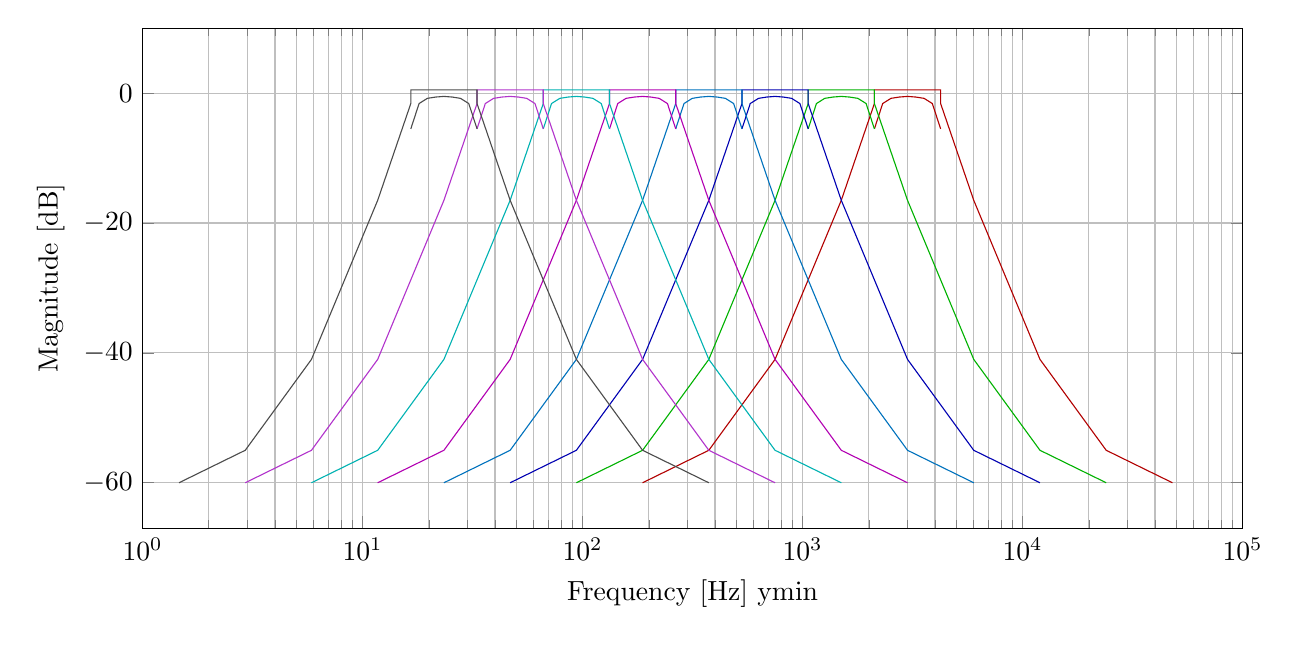
\begin{tikzpicture}

\begin{axis}[%
width=5.5in,
height=2.5in,
at={(0.758in,0.481in)},
scale only axis,
unbounded coords=jump,
xmode=log,
xmin=1,
xmax=100000,
xminorticks=true,
xmajorgrids,
xminorgrids,
ylabel={Magnitude [dB]},
xlabel={Frequency [Hz]}
ymin=-60,
ymax=10,
ymajorgrids,
axis background/.style={fill=white}
]
\addplot [color=black!30!red,solid,forget plot]
  table[row sep=crcr]{%
187.5	-60\\
375	-55\\
750	-41\\
1500	-16.5\\
2121.32034355964	-1.6\\
2121.32034355964	0.5\\
2313.31623811191	0.5\\
2522.68924576114	0.5\\
2751.01212961401	0.5\\
3000	0.5\\
3271.52319799577	0.5\\
3567.62134500816	0.5\\
3890.51866395303	0.5\\
4242.64068711929	0.5\\
4242.64068711929	-1.6\\
6000	-16.5\\
12000	-41\\
24000	-55\\
48000	-60\\
};
\addplot [color=black!30!red,solid,forget plot]
  table[row sep=crcr]{%
187.5	-inf\\
375	-inf\\
750	-inf\\
1500	-inf\\
2121.32034355964	-5.5\\
2121.32034355964	-5.5\\
2313.31623811191	-1.6\\
2522.68924576114	-0.8\\
2751.01212961401	-0.6\\
3000	-0.5\\
3271.52319799577	-0.6\\
3567.62134500816	-0.8\\
3890.51866395303	-1.6\\
4242.64068711929	-5.5\\
4242.64068711929	-5.5\\
6000	-inf\\
12000	-inf\\
24000	-inf\\
48000	-inf\\
};
\addplot [color=black!30!green,solid,forget plot]
  table[row sep=crcr]{%
93.75	-60\\
187.5	-55\\
375	-41\\
750	-16.5\\
1060.66017177982	-1.6\\
1060.66017177982	0.5\\
1156.65811905596	0.5\\
1261.34462288057	0.5\\
1375.50606480701	0.5\\
1500	0.5\\
1635.76159899789	0.5\\
1783.81067250408	0.5\\
1945.25933197651	0.5\\
2121.32034355964	0.5\\
2121.32034355964	-1.6\\
3000	-16.5\\
6000	-41\\
12000	-55\\
24000	-60\\
};
\addplot [color=black!30!green,solid,forget plot]
  table[row sep=crcr]{%
93.75	-inf\\
187.5	-inf\\
375	-inf\\
750	-inf\\
1060.66017177982	-5.5\\
1060.66017177982	-5.5\\
1156.65811905596	-1.6\\
1261.34462288057	-0.8\\
1375.50606480701	-0.6\\
1500	-0.5\\
1635.76159899789	-0.6\\
1783.81067250408	-0.8\\
1945.25933197651	-1.6\\
2121.32034355964	-5.5\\
2121.32034355964	-5.5\\
3000	-inf\\
6000	-inf\\
12000	-inf\\
24000	-inf\\
};
\addplot [color=black!30!blue,solid,forget plot]
  table[row sep=crcr]{%
46.875	-60\\
93.75	-55\\
187.5	-41\\
375	-16.5\\
530.330085889911	-1.6\\
530.330085889911	0.5\\
578.329059527978	0.5\\
630.672311440286	0.5\\
687.753032403503	0.5\\
750	0.5\\
817.880799498943	0.5\\
891.905336252041	0.5\\
972.629665988257	0.5\\
1060.66017177982	0.5\\
1060.66017177982	-1.6\\
1500	-16.5\\
3000	-41\\
6000	-55\\
12000	-60\\
};
\addplot [color=black!30!blue,solid,forget plot]
  table[row sep=crcr]{%
46.875	-inf\\
93.75	-inf\\
187.5	-inf\\
375	-inf\\
530.330085889911	-5.5\\
530.330085889911	-5.5\\
578.329059527978	-1.6\\
630.672311440286	-0.8\\
687.753032403503	-0.6\\
750	-0.5\\
817.880799498943	-0.6\\
891.905336252041	-0.8\\
972.629665988257	-1.6\\
1060.66017177982	-5.5\\
1060.66017177982	-5.5\\
1500	-inf\\
3000	-inf\\
6000	-inf\\
12000	-inf\\
};
\addplot [color=mycolor1,solid,forget plot]
  table[row sep=crcr]{%
23.4375	-60\\
46.875	-55\\
93.75	-41\\
187.5	-16.5\\
265.165042944955	-1.6\\
265.165042944955	0.5\\
289.164529763989	0.5\\
315.336155720143	0.5\\
343.876516201752	0.5\\
375	0.5\\
408.940399749472	0.5\\
445.95266812602	0.5\\
486.314832994129	0.5\\
530.330085889911	0.5\\
530.330085889911	-1.6\\
750	-16.5\\
1500	-41\\
3000	-55\\
6000	-60\\
};
\addplot [color=mycolor1,solid,forget plot]
  table[row sep=crcr]{%
23.4375	-inf\\
46.875	-inf\\
93.75	-inf\\
187.5	-inf\\
265.165042944955	-5.5\\
265.165042944955	-5.5\\
289.164529763989	-1.6\\
315.336155720143	-0.8\\
343.876516201752	-0.6\\
375	-0.5\\
408.940399749472	-0.6\\
445.95266812602	-0.8\\
486.314832994129	-1.6\\
530.330085889911	-5.5\\
530.330085889911	-5.5\\
750	-inf\\
1500	-inf\\
3000	-inf\\
6000	-inf\\
};
\addplot [color=mycolor2,solid,forget plot]
  table[row sep=crcr]{%
11.71875	-60\\
23.4375	-55\\
46.875	-41\\
93.75	-16.5\\
132.582521472478	-1.6\\
132.582521472478	0.5\\
144.582264881994	0.5\\
157.668077860071	0.5\\
171.938258100876	0.5\\
187.5	0.5\\
204.470199874736	0.5\\
222.97633406301	0.5\\
243.157416497064	0.5\\
265.165042944955	0.5\\
265.165042944955	-1.6\\
375	-16.5\\
750	-41\\
1500	-55\\
3000	-60\\
};
\addplot [color=mycolor2,solid,forget plot]
  table[row sep=crcr]{%
11.71875	-inf\\
23.4375	-inf\\
46.875	-inf\\
93.75	-inf\\
132.582521472478	-5.5\\
132.582521472478	-5.5\\
144.582264881994	-1.6\\
157.668077860071	-0.8\\
171.938258100876	-0.6\\
187.5	-0.5\\
204.470199874736	-0.6\\
222.97633406301	-0.8\\
243.157416497064	-1.6\\
265.165042944955	-5.5\\
265.165042944955	-5.5\\
375	-inf\\
750	-inf\\
1500	-inf\\
3000	-inf\\
};
\addplot [color=mycolor3,solid,forget plot]
  table[row sep=crcr]{%
5.859375	-60\\
11.71875	-55\\
23.4375	-41\\
46.875	-16.5\\
66.2912607362388	-1.6\\
66.2912607362388	0.5\\
72.2911324409972	0.5\\
78.8340389300357	0.5\\
85.9691290504379	0.5\\
93.75	0.5\\
102.235099937368	0.5\\
111.488167031505	0.5\\
121.578708248532	0.5\\
132.582521472478	0.5\\
132.582521472478	-1.6\\
187.5	-16.5\\
375	-41\\
750	-55\\
1500	-60\\
};
\addplot [color=mycolor3,solid,forget plot]
  table[row sep=crcr]{%
5.859375	-inf\\
11.71875	-inf\\
23.4375	-inf\\
46.875	-inf\\
66.2912607362388	-5.5\\
66.2912607362388	-5.5\\
72.2911324409972	-1.6\\
78.8340389300357	-0.8\\
85.9691290504379	-0.6\\
93.75	-0.5\\
102.235099937368	-0.6\\
111.488167031505	-0.8\\
121.578708248532	-1.6\\
132.582521472478	-5.5\\
132.582521472478	-5.5\\
187.5	-inf\\
375	-inf\\
750	-inf\\
1500	-inf\\
};
\addplot [color=mycolor4,solid,forget plot]
  table[row sep=crcr]{%
2.9296875	-60\\
5.859375	-55\\
11.71875	-41\\
23.4375	-16.5\\
33.1456303681194	-1.6\\
33.1456303681194	0.5\\
36.1455662204986	0.5\\
39.4170194650179	0.5\\
42.984564525219	0.5\\
46.875	0.5\\
51.117549968684	0.5\\
55.7440835157526	0.5\\
60.7893541242661	0.5\\
66.2912607362388	0.5\\
66.2912607362388	-1.6\\
93.75	-16.5\\
187.5	-41\\
375	-55\\
750	-60\\
};
\addplot [color=mycolor4,solid,forget plot]
  table[row sep=crcr]{%
2.9296875	-inf\\
5.859375	-inf\\
11.71875	-inf\\
23.4375	-inf\\
33.1456303681194	-5.5\\
33.1456303681194	-5.5\\
36.1455662204986	-1.6\\
39.4170194650179	-0.8\\
42.984564525219	-0.6\\
46.875	-0.5\\
51.117549968684	-0.6\\
55.7440835157526	-0.8\\
60.7893541242661	-1.6\\
66.2912607362388	-5.5\\
66.2912607362388	-5.5\\
93.75	-inf\\
187.5	-inf\\
375	-inf\\
750	-inf\\
};
\addplot [color=white!30!black,solid,forget plot]
  table[row sep=crcr]{%
1.46484375	-60\\
2.9296875	-55\\
5.859375	-41\\
11.71875	-16.5\\
16.5728151840597	-1.6\\
16.5728151840597	0.5\\
18.0727831102493	0.5\\
19.7085097325089	0.5\\
21.4922822626095	0.5\\
23.4375	0.5\\
25.558774984342	0.5\\
27.8720417578763	0.5\\
30.394677062133	0.5\\
33.1456303681194	0.5\\
33.1456303681194	-1.6\\
46.875	-16.5\\
93.75	-41\\
187.5	-55\\
375	-60\\
};
\addplot [color=white!30!black,solid,forget plot]
  table[row sep=crcr]{%
1.46484375	-inf\\
2.9296875	-inf\\
5.859375	-inf\\
11.71875	-inf\\
16.5728151840597	-5.5\\
16.5728151840597	-5.5\\
18.0727831102493	-1.6\\
19.7085097325089	-0.8\\
21.4922822626095	-0.6\\
23.4375	-0.5\\
25.558774984342	-0.6\\
27.8720417578763	-0.8\\
30.394677062133	-1.6\\
33.1456303681194	-5.5\\
33.1456303681194	-5.5\\
46.875	-inf\\
93.75	-inf\\
187.5	-inf\\
375	-inf\\
};
\end{axis}
\end{tikzpicture}%
	\caption{Overview of all band requirements}
	\label{fig:allBands}
\end{figure}
The reason for downsampling seven times and not more or less is because of several reasons. Firstly the bandwidth of the decimation filter must not be influenced by the interpolation filter which would give a non flat frequency response so every band is set to have a center frequency 1/16 of Fs, secondly the lower the center frequency in relation to Fs the higher the filter order which is desired as low as possible, lastly increasing the number of downsamples increases the delay of the system which is not desired in relation to real time applications.       
\todo[inline]{Skal det være mere begrundet? skal vi skrive at det er baseret på trial and error senere i forløbet?}

Because there will be downsampled by two for every octave band the following relation can be made between a band and Fs as seen on \autoref{fig:relFsBand}.
\begin{figure}[H]
	\centering
	\tikzsetnextfilename{relativeFsBand}
	% This file was created by matlab2tikz.
%
%The latest updates can be retrieved from
%  http://www.mathworks.com/matlabcentral/fileexchange/22022-matlab2tikz-matlab2tikz
%where you can also make suggestions and rate matlab2tikz.
%
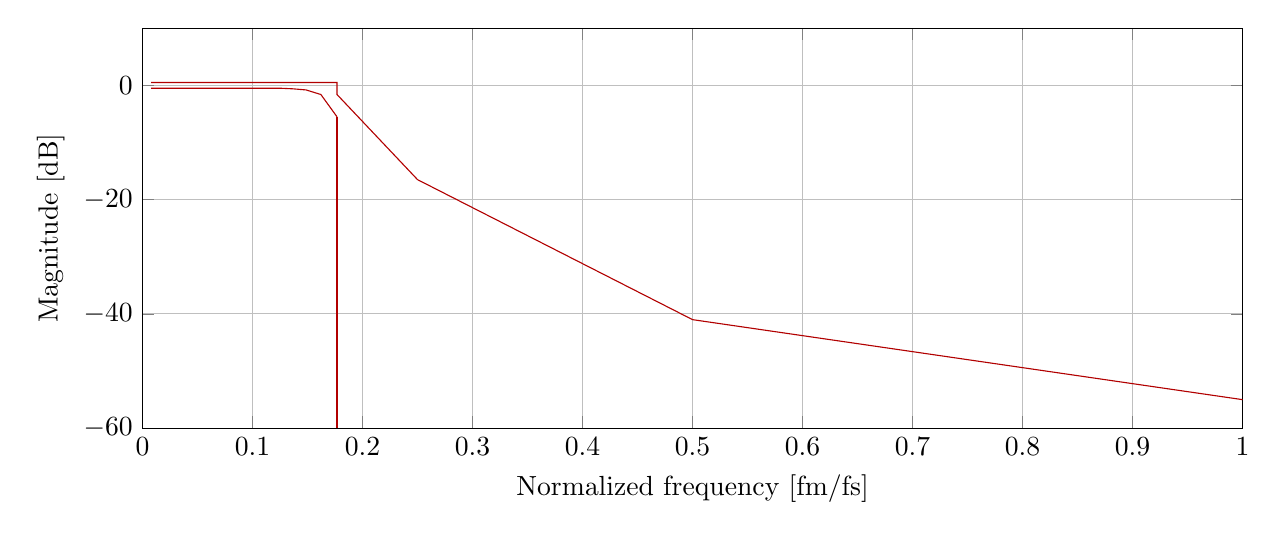
\begin{tikzpicture}

\begin{axis}[%
width=5.5in,
height=2in,
at={(0.758in,0.481in)},
scale only axis,
unbounded coords=jump,
xmin=0,
xmax=1,
xlabel={Normalized frequency [fm/fs]},
xmajorgrids,
ymin=-60,
ymax=10,
ylabel={Magnitude [dB]},
ymajorgrids,
axis background/.style={fill=white}
]
\addplot [color=black!30!red,solid,forget plot]
  table[row sep=crcr]{%
0.1768	-5.5\\
0.1768	-60\\
};
\addplot [color=black!30!red,solid,forget plot]
  table[row sep=crcr]{%
0.0078125	0.5\\
0.015625	0.5\\
0.03125	0.5\\
0.0625	0.5\\
0.0883883476483184	0.5\\
0.0883883476483184	0.5\\
0.0963881765879963	0.5\\
0.105112051906714	0.5\\
0.114625505400584	0.5\\
0.125	0.5\\
0.136313466583157	0.5\\
0.14865088937534	0.5\\
0.162104944331376	0.5\\
0.176776695296637	0.5\\
0.176776695296637	-1.6\\
0.25	-16.5\\
0.5	-41\\
1	-55\\
2	-60\\
};
\addplot [color=black!30!red,solid,forget plot]
  table[row sep=crcr]{%
0.0078125	-0.5\\
0.015625	-0.5\\
0.03125	-0.5\\
0.0625	-0.5\\
0.0883883476483184	-0.5\\
0.0883883476483184	-0.5\\
0.0963881765879963	-0.5\\
0.105112051906714	-0.5\\
0.114625505400584	-0.5\\
0.125	-0.5\\
0.136313466583157	-0.6\\
0.14865088937534	-0.8\\
0.162104944331376	-1.6\\
0.176776695296637	-5.5\\
0.176776695296637	-5.5\\
0.25	-inf\\
0.5	-inf\\
1	-inf\\
2	-inf\\
};
\end{axis}
\end{tikzpicture}%
	\caption{Band relative to Fs}
	\label{fig:relFsBand}
\end{figure}

From \autoref{fig:relFsBand} two points are selected giving the following specifications to the lowpass filter:

$\omega_{pass}=3.000\textrm{ Hz }\cdot 2/Fs=0.1250 \enhed{rad/sample}$\\
$A_{pass}=-1 \enhed{dB}$\\
$\omega_{stop}=6.500\textrm{ Hz }\cdot 2/Fs=0.2708 \enhed{rad/sample}$\\
$A_{stop}=-60 \enhed{dB}$

The design method used for designing the filter is the Kaiser window method, explained in detail in \autoref{app:FIR_theory}. The reason for using the Kaiser window method is that it gives the approximate order of the filter and the beta value of the window applied to impulse reponse. This means that no trial and error method is needed to meet the requierments of the filter.

With the specification stated and using the matlab script explained in \autoref{app:FIR_Matlab} which uses the FIR theoy explained in \autoref{app:FIR_theory} about the Kaiser window method, general FIR theory and deriving the coefficients of the filter, the following filter is given with quantisized coefficients, see \autoref{fig:band1_filt} for magnitude response and \autoref{fig:band1_filtPhase} for phase response. The order of the filter is 50, it is a type 1 FIR filter and has linear phase which means that the group delay is constant at 25 samples.  

\begin{figure}[H]
\centering
	\tikzsetnextfilename{Band1Filt}
	% This file was created by matlab2tikz.
%
%The latest updates can be retrieved from
%  http://www.mathworks.com/matlabcentral/fileexchange/22022-matlab2tikz-matlab2tikz
%where you can also make suggestions and rate matlab2tikz.
%
\definecolor{mycolor1}{rgb}{0.00000,0.44700,0.74100}%
%
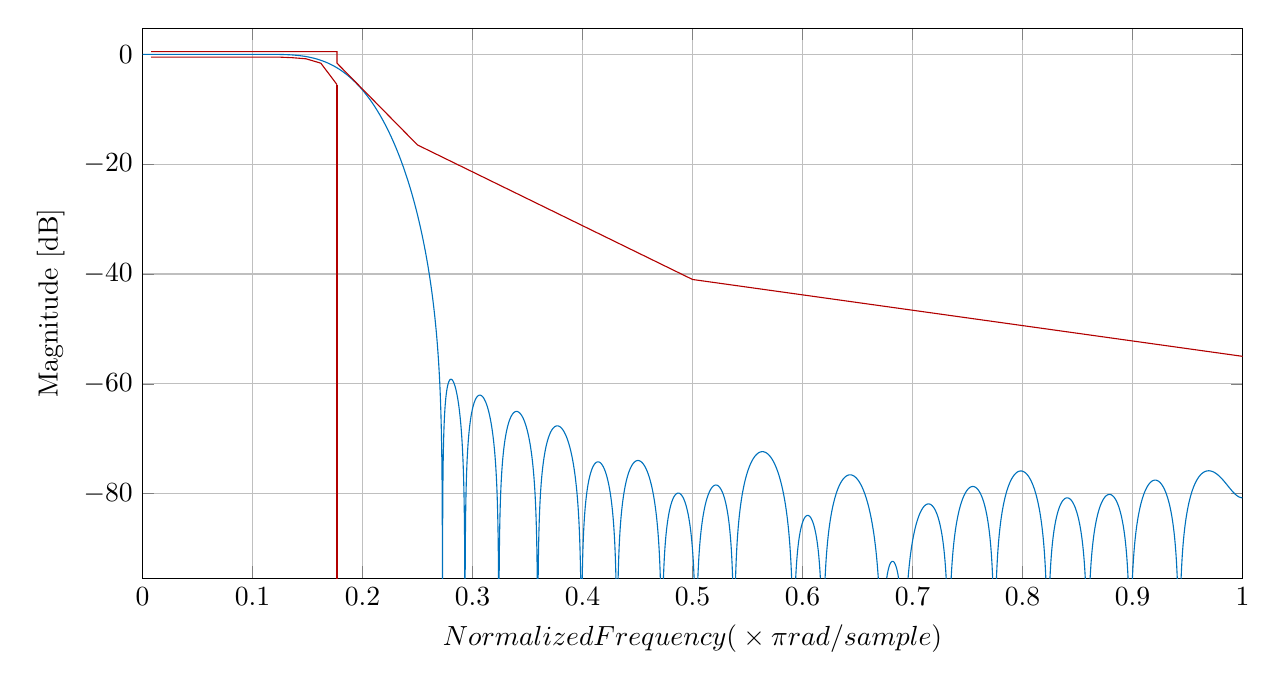
\begin{tikzpicture}

\begin{axis}[%
width=5.5in,
height=2.75in,
at={(1.281in,0.447in)},
scale only axis,
unbounded coords=jump,
xmin=0,
xmax=1,
xlabel={$\text{Normalized Frequency (}\times\pi\text{ rad/sample)}$},
xmajorgrids,
ymin=-95.4207080394785,
ymax=4.7713185812425,
ylabel={Magnitude [dB]},
ymajorgrids,
axis background/.style={fill=white},
]
\addplot [color=mycolor1,solid,forget plot]
  table[row sep=crcr]{%
0	0.002385323281203\\
0.0001220703125	0.00238515620543467\\
0.000244140625	0.00238465500069651\\
0.0003662109375	0.00238381973514379\\
0.00048828125	0.00238265052200859\\
0.0006103515625	0.00238114752011143\\
0.000732421875	0.00237931093340649\\
0.0008544921875	0.00237714101120901\\
0.0009765625	0.00237463804796789\\
0.0010986328125	0.00237180238360679\\
0.001220703125	0.00236863440289881\\
0.0013427734375	0.00236513453592124\\
0.00146484375	0.00236130325782824\\
0.0015869140625	0.00235714108868024\\
0.001708984375	0.00235264859355766\\
0.0018310546875	0.00234782638233355\\
0.001953125	0.00234267510978725\\
0.0020751953125	0.0023371954752065\\
0.002197265625	0.00233138822267165\\
0.0023193359375	0.00232525414077145\\
0.00244140625	0.00231879406231883\\
0.0025634765625	0.00231200886469196\\
0.002685546875	0.00230489946932266\\
0.0028076171875	0.00229746684169641\\
0.0029296875	0.00228971199135231\\
0.0030517578125	0.00228163597159892\\
0.003173828125	0.00227323987945738\\
0.0032958984375	0.00226452485554773\\
0.00341796875	0.00225549208369102\\
0.0035400390625	0.00224614279125035\\
0.003662109375	0.00223647824844875\\
0.0037841796875	0.00222649976865341\\
0.00390625	0.00221620870775041\\
0.0040283203125	0.00220560646437207\\
0.004150390625	0.00219469447961274\\
0.0042724609375	0.0021834742366309\\
0.00439453125	0.00217194726076286\\
0.0045166015625	0.002160115119068\\
0.004638671875	0.00214797942038558\\
0.0047607421875	0.00213554181482323\\
0.0048828125	0.0021228039938137\\
0.0050048828125	0.00210976768977389\\
0.005126953125	0.00209643467593423\\
0.0052490234375	0.00208280676594086\\
0.00537109375	0.00206888581396925\\
0.0054931640625	0.00205467371409895\\
0.005615234375	0.00204017240037047\\
0.0057373046875	0.0020253838462736\\
0.005859375	0.00201031006480434\\
0.0059814453125	0.00199495310783959\\
0.006103515625	0.00197931506625082\\
0.0062255859375	0.0019633980693925\\
0.00634765625	0.00194720428476103\\
0.0064697265625	0.00193073591810844\\
0.006591796875	0.00191399521258973\\
0.0067138671875	0.00189698444904707\\
0.0068359375	0.00187970594521403\\
0.0069580078125	0.00186216205582923\\
0.007080078125	0.00184435517201109\\
0.0072021484375	0.00182628772120097\\
0.00732421875	0.00180796216670842\\
0.0074462890625	0.0017893810073133\\
0.007568359375	0.00177054677726574\\
0.0076904296875	0.00175146204554721\\
0.0078125	0.00173212941587053\\
0.0079345703125	0.00171255152616823\\
0.008056640625	0.00169273104819467\\
0.0081787109375	0.00167267068746924\\
0.00830078125	0.0016523731825373\\
0.0084228515625	0.00163184130502714\\
0.008544921875	0.0016110778589109\\
0.0086669921875	0.00159008568039098\\
0.0087890625	0.00156886763744524\\
0.0089111328125	0.00154742662942908\\
0.009033203125	0.00152576558673445\\
0.0091552734375	0.00150388747044872\\
0.00927734375	0.00148179527189996\\
0.0093994140625	0.00145949201237272\\
0.009521484375	0.00143698074248277\\
0.0096435546875	0.00141426454212024\\
0.009765625	0.00139134651976747\\
0.0098876953125	0.00136822981221485\\
0.010009765625	0.00134491758416289\\
0.0101318359375	0.00132141302776745\\
0.01025390625	0.00129771936218503\\
0.0103759765625	0.00127383983328855\\
0.010498046875	0.00124977771315571\\
0.0106201171875	0.00122553629967115\\
0.0107421875	0.00120111891595798\\
0.0108642578125	0.0011765289102641\\
0.010986328125	0.00115176965510955\\
0.0111083984375	0.00112684454722967\\
0.01123046875	0.00110175700689297\\
0.0113525390625	0.00107651047756008\\
0.011474609375	0.00105110842537215\\
0.0115966796875	0.00102555433869611\\
0.01171875	0.000999851727783607\\
0.0118408203125	0.000974004124145722\\
0.011962890625	0.000948015080211917\\
0.0120849609375	0.000921888168818441\\
0.01220703125	0.000895626982753583\\
0.0123291015625	0.000869235134302926\\
0.012451171875	0.000842716254624065\\
0.0125732421875	0.000816073993576083\\
0.0126953125	0.000789312018923738\\
0.0128173828125	0.000762434016110092\\
0.012939453125	0.000735443687460702\\
0.0130615234375	0.000708344752126777\\
0.01318359375	0.000681140945175684\\
0.0133056640625	0.000653836017420417\\
0.013427734375	0.000626433734680631\\
0.0135498046875	0.000598937877441585\\
0.013671875	0.000571352240285705\\
0.0137939453125	0.000543680631437837\\
0.013916015625	0.000515926872139971\\
0.0140380859375	0.000488094796423866\\
0.01416015625	0.000460188250258398\\
0.0142822265625	0.000432211091322188\\
0.014404296875	0.000404167188264637\\
0.0145263671875	0.000376060420308022\\
0.0146484375	0.000347894676849592\\
0.0147705078125	0.000319673856722602\\
0.014892578125	0.000291401867798413\\
0.0150146484375	0.000263082626418054\\
0.01513671875	0.00023472005699432\\
0.0152587890625	0.000206318091272806\\
0.015380859375	0.000177880668047692\\
0.0155029296875	0.000149411732422777\\
0.015625	0.000120915235413577\\
0.0157470703125	9.23951334357298e-05\\
0.015869140625	6.38553876228798e-05\\
0.0159912109375	3.52999635424567e-05\\
0.01611328125	6.73283045671269e-06\\
0.0162353515625	-2.18420391888685e-05\\
0.016357421875	-5.04206701634757e-05\\
0.0164794921875	-7.89990851330913e-05\\
0.0166015625	-0.000107573305172082\\
0.0167236328125	-0.000136139350047415\\
0.016845703125	-0.000164693239241842\\
0.0169677734375	-0.00019323099201074\\
0.01708984375	-0.000221748628234764\\
0.0172119140625	-0.000250242168704062\\
0.017333984375	-0.000278707636027775\\
0.0174560546875	-0.000307141054690874\\
0.017578125	-0.000335538451963657\\
0.0177001953125	-0.000363895858299657\\
0.017822265625	-0.000392209307847224\\
0.0179443359375	-0.000420474839074814\\
0.01806640625	-0.000448688495225724\\
0.0181884765625	-0.000476846324943381\\
0.018310546875	-0.00050494438272608\\
0.0184326171875	-0.000532978729438582\\
0.0185546875	-0.000560945432937388\\
0.0186767578125	-0.000588840568696014\\
0.018798828125	-0.000616660220032372\\
0.0189208984375	-0.000644400478904572\\
0.01904296875	-0.000672057446479357\\
0.0191650390625	-0.000699627233359479\\
0.019287109375	-0.000727105960436347\\
0.0194091796875	-0.000754489759344779\\
0.01953125	-0.000781774772860899\\
0.0196533203125	-0.00080895715564111\\
0.019775390625	-0.00083603307444946\\
0.0198974609375	-0.000862998709010299\\
0.02001953125	-0.00088985025246302\\
0.0201416015625	-0.000916583911646285\\
0.020263671875	-0.00094319590800751\\
0.0203857421875	-0.00096968247771656\\
0.0205078125	-0.000996039872518395\\
0.0206298828125	-0.00102226436018782\\
0.020751953125	-0.0010483522248137\\
0.0208740234375	-0.00107429976765161\\
0.02099609375	-0.00110010330740806\\
0.0211181640625	-0.00112575918086577\\
0.021240234375	-0.00115126374339525\\
0.0213623046875	-0.00117661336929586\\
0.021484375	-0.0012018044526485\\
0.0216064453125	-0.00122683340742924\\
0.021728515625	-0.00125169666830516\\
0.0218505859375	-0.00127639069108909\\
0.02197265625	-0.001300911952967\\
0.0220947265625	-0.00132525695352115\\
0.022216796875	-0.00134942221467327\\
0.0223388671875	-0.00137340428153721\\
0.0224609375	-0.00139719972275998\\
0.0225830078125	-0.00142080513114706\\
0.022705078125	-0.0014442171239466\\
0.0228271484375	-0.00146743234347468\\
0.02294921875	-0.0014904474575701\\
0.0230712890625	-0.00151325916010592\\
0.023193359375	-0.00153586417133056\\
0.0233154296875	-0.00155825923854991\\
0.0234375	-0.00158044113641154\\
0.0235595703125	-0.00160240666741629\\
0.023681640625	-0.00162415266248672\\
0.0238037109375	-0.001645675981365\\
0.02392578125	-0.00166697351295397\\
0.0240478515625	-0.00168804217588558\\
0.024169921875	-0.00170887891908933\\
0.0242919921875	-0.00172948072201962\\
0.0244140625	-0.00174984459516736\\
0.0245361328125	-0.00176996758062842\\
0.024658203125	-0.00178984675221727\\
0.0247802734375	-0.00180947921643337\\
0.02490234375	-0.00182886211234745\\
0.0250244140625	-0.00184799261228363\\
0.025146484375	-0.00186686792238788\\
0.0252685546875	-0.001885485282628\\
0.025390625	-0.0019038419677031\\
0.0255126953125	-0.00192193528698681\\
0.025634765625	-0.00193976258526618\\
0.0257568359375	-0.00195732124313963\\
0.02587890625	-0.00197460867707377\\
0.0260009765625	-0.00199162234019923\\
0.026123046875	-0.00200835972248115\\
0.0262451171875	-0.00202481835128765\\
0.0263671875	-0.00204099579133299\\
0.0264892578125	-0.00205688964575756\\
0.026611328125	-0.00207249755578687\\
0.0267333984375	-0.00208781720164097\\
0.02685546875	-0.00210284630253454\\
0.0269775390625	-0.00211758261724526\\
0.027099609375	-0.00213202394439804\\
0.0272216796875	-0.0021461681228061\\
0.02734375	-0.00216001303186886\\
0.0274658203125	-0.00217355659185614\\
0.027587890625	-0.00218679676419242\\
0.0277099609375	-0.00219973155202524\\
0.02783203125	-0.00221235900016836\\
0.0279541015625	-0.00222467719572705\\
0.028076171875	-0.00223668426843915\\
0.0281982421875	-0.00224837839073189\\
0.0283203125	-0.00225975777811982\\
0.0284423828125	-0.0022708206897164\\
0.028564453125	-0.00228156542817715\\
0.0286865234375	-0.0022919903403249\\
0.02880859375	-0.0023020938172067\\
0.0289306640625	-0.0023118742944348\\
0.029052734375	-0.00232133025252779\\
0.0291748046875	-0.00233046021702421\\
0.029296875	-0.00233926275899421\\
0.0294189453125	-0.0023477364950395\\
0.029541015625	-0.00235588008769128\\
0.0296630859375	-0.00236369224552391\\
0.02978515625	-0.00237117172355283\\
0.0299072265625	-0.00237831732351879\\
0.030029296875	-0.0023851278937741\\
0.0301513671875	-0.00239160232990798\\
0.0302734375	-0.00239773957468969\\
0.0303955078125	-0.00240353861840958\\
0.030517578125	-0.00240899849904963\\
0.0306396484375	-0.00241411830245397\\
0.03076171875	-0.00241889716261312\\
0.0308837890625	-0.00242333426177765\\
0.031005859375	-0.0024274288305719\\
0.0311279296875	-0.00243118014827814\\
0.03125	-0.00243458754306403\\
0.0313720703125	-0.00243765039192567\\
0.031494140625	-0.00244036812108561\\
0.0316162109375	-0.00244274020593593\\
0.03173828125	-0.00244476617137934\\
0.0318603515625	-0.00244644559177232\\
0.031982421875	-0.00244777809115249\\
0.0321044921875	-0.002448763343466\\
0.0322265625	-0.00244940107251068\\
0.0323486328125	-0.00244969105204973\\
0.032470703125	-0.00244963310615276\\
0.0325927734375	-0.00244922710896844\\
0.03271484375	-0.00244847298506556\\
0.0328369140625	-0.00244737070943302\\
0.032958984375	-0.00244592030753665\\
0.0330810546875	-0.00244412185537612\\
0.033203125	-0.0024419754797691\\
0.0333251953125	-0.00243948135795335\\
0.033447265625	-0.00243663971821206\\
0.0335693359375	-0.00243345083941904\\
0.03369140625	-0.00242991505143664\\
0.0338134765625	-0.00242603273483155\\
0.033935546875	-0.00242180432132955\\
0.0340576171875	-0.00241723029330387\\
0.0341796875	-0.00241231118434371\\
0.0343017578125	-0.00240704757874255\\
0.034423828125	-0.00240144011183929\\
0.0345458984375	-0.00239548947007506\\
0.03466796875	-0.00238919639048163\\
0.0347900390625	-0.00238256166136352\\
0.034912109375	-0.00237558612161592\\
0.0350341796875	-0.00236827066112255\\
0.03515625	-0.00236061622064199\\
0.0352783203125	-0.0023526237915803\\
0.035400390625	-0.00234429441604789\\
0.0355224609375	-0.00233562918691632\\
0.03564453125	-0.00232662924753413\\
0.0357666015625	-0.00231729579178364\\
0.035888671875	-0.00230763006408097\\
0.0360107421875	-0.00229763335897815\\
0.0361328125	-0.00228730702150415\\
0.0362548828125	-0.00227665244659647\\
0.036376953125	-0.00226567107949904\\
0.0364990234375	-0.00225436441508009\\
0.03662109375	-0.00224273399823005\\
0.0367431640625	-0.00223078142346367\\
0.036865234375	-0.00221850833469261\\
0.0369873046875	-0.00220591642545287\\
0.037109375	-0.00219300743833628\\
0.0372314453125	-0.00217978316510425\\
0.037353515625	-0.00216624544640354\\
0.0374755859375	-0.00215239617165253\\
0.03759765625	-0.00213823727892759\\
0.0377197265625	-0.00212377075445147\\
0.037841796875	-0.00210899863299119\\
0.0379638671875	-0.00209392299706224\\
0.0380859375	-0.00207854597704227\\
0.0382080078125	-0.00206286975094372\\
0.038330078125	-0.0020468965441296\\
0.0384521484375	-0.00203062862914294\\
0.03857421875	-0.00201406832536577\\
0.0386962890625	-0.0019972179989054\\
0.038818359375	-0.00198008006236705\\
0.0389404296875	-0.00196265697445597\\
0.0390625	-0.00194495123980687\\
0.0391845703125	-0.00192696540869974\\
0.039306640625	-0.00190870207694616\\
0.0394287109375	-0.00189016388526397\\
0.03955078125	-0.00187135351933421\\
0.0396728515625	-0.00185227370934626\\
0.039794921875	-0.00183292722977058\\
0.0399169921875	-0.00181331689884701\\
0.0400390625	-0.00179344557864169\\
0.0401611328125	-0.00177331617442178\\
0.040283203125	-0.00175293163448487\\
0.0404052734375	-0.00173229494964744\\
0.04052734375	-0.00171140915324486\\
0.0406494140625	-0.00169027732044924\\
0.040771484375	-0.00166890256804209\\
0.0408935546875	-0.00164728805413006\\
0.041015625	-0.00162543697774709\\
0.0411376953125	-0.00160335257839961\\
0.041259765625	-0.00158103813578236\\
0.0413818359375	-0.00155849696932364\\
0.04150390625	-0.0015357324379579\\
0.0416259765625	-0.00151274793944367\\
0.041748046875	-0.00148954691024983\\
0.0418701171875	-0.00146613282504404\\
0.0419921875	-0.00144250919629485\\
0.0421142578125	-0.00141867957364639\\
0.042236328125	-0.00139464754391838\\
0.0423583984375	-0.00137041673031035\\
0.04248046875	-0.00134599079211739\\
0.0426025390625	-0.00132137342427541\\
0.042724609375	-0.00129656835684955\\
0.0428466796875	-0.00127157935469313\\
0.04296875	-0.00124641021693606\\
0.0430908203125	-0.00122106477641637\\
0.043212890625	-0.00119554689933921\\
0.0433349609375	-0.00116986048493573\\
0.04345703125	-0.00114400946455362\\
0.0435791015625	-0.00111799780154342\\
0.043701171875	-0.00109182949069009\\
0.0438232421875	-0.00106550855758769\\
0.0439453125	-0.00103903905829839\\
0.0440673828125	-0.00101242507867028\\
0.044189453125	-0.000985670733996358\\
0.0443115234375	-0.000958780168389239\\
0.04443359375	-0.000931757554269552\\
0.0445556640625	-0.000904607091854359\\
0.044677734375	-0.000877333008645564\\
0.0447998046875	-0.000849939558804635\\
0.044921875	-0.000822431022641013\\
0.0450439453125	-0.000794811706214205\\
0.045166015625	-0.000767085940424295\\
0.0452880859375	-0.000739258080955096\\
0.04541015625	-0.000711332507080442\\
0.0455322265625	-0.00068331362177787\\
0.045654296875	-0.000655205850591756\\
0.0457763671875	-0.000627013641349095\\
0.0458984375	-0.000598741463477381\\
0.0460205078125	-0.000570393807493019\\
0.046142578125	-0.000541975184319199\\
0.0462646484375	-0.000513490124717464\\
0.04638671875	-0.000484943178662434\\
0.0465087890625	-0.000456338914830212\\
0.046630859375	-0.000427681919916267\\
0.0467529296875	-0.000398976798010153\\
0.046875	-0.000370228170027076\\
0.0469970703125	-0.000341440672968929\\
0.047119140625	-0.000312618959469546\\
0.0472412109375	-0.000283767696998893\\
0.04736328125	-0.000254891567465165\\
0.0474853515625	-0.000225995266191603\\
0.047607421875	-0.000197083501632278\\
0.0477294921875	-0.000168160994633126\\
0.0478515625	-0.000139232477636142\\
0.0479736328125	-0.000110302694281472\\
0.048095703125	-8.13763983842364e-05\\
0.0482177734375	-5.24583537071521e-05\\
0.04833984375	-2.35533330510407e-05\\
0.0484619140625	5.33388254098099e-06\\
0.048583984375	3.41985040677173e-05\\
0.0487060546875	6.30357355930755e-05\\
0.048828125	9.18407747576566e-05\\
0.0489501953125	0.000120608813460876\\
0.049072265625	0.000149335038599929\\
0.0491943359375	0.000178014632695067\\
0.04931640625	0.000206642774685406\\
0.0494384765625	0.000235214640440518\\
0.049560546875	0.000263725403556236\\
0.0496826171875	0.000292170236036782\\
0.0498046875	0.000320544309147408\\
0.0499267578125	0.000348842793698623\\
0.050048828125	0.000377060861239897\\
0.0501708984375	0.000405193684400729\\
0.05029296875	0.000433236437800133\\
0.0504150390625	0.000461184298558237\\
0.050537109375	0.00048903244731946\\
0.0506591796875	0.000516776068593572\\
0.05078125	0.000544410351835722\\
0.0509033203125	0.000571930491730654\\
0.051025390625	0.000599331689386418\\
0.0511474609375	0.000626609152618585\\
0.05126953125	0.00065375809708712\\
0.0513916015625	0.000680773746580599\\
0.051513671875	0.000707651334039383\\
0.0516357421875	0.000734386102294593\\
0.0517578125	0.00076097330452285\\
0.0518798828125	0.000787408205326301\\
0.052001953125	0.00081368608101684\\
0.0521240234375	0.000839802220866659\\
0.05224609375	0.000865751927392466\\
0.0523681640625	0.000891530517378669\\
0.052490234375	0.00091713332233212\\
0.0526123046875	0.000942555689618985\\
0.052734375	0.000967792982635274\\
0.0528564453125	0.000992840582057397\\
0.052978515625	0.00101769388629691\\
0.0531005859375	0.00104234831229633\\
0.05322265625	0.00106679929626807\\
0.0533447265625	0.00109104229443346\\
0.053466796875	0.00111507278364797\\
0.0535888671875	0.00113888626236758\\
0.0537109375	0.00116247825098981\\
0.0538330078125	0.00118584429316115\\
0.053955078125	0.00120897995577707\\
0.0540771484375	0.00123188083051673\\
0.05419921875	0.00125454253378621\\
0.0543212890625	0.00127696070802585\\
0.054443359375	0.00129913102216506\\
0.0545654296875	0.00132104917247489\\
0.0546875	0.00134271088313653\\
0.0548095703125	0.0013641119071508\\
0.054931640625	0.00138524802679285\\
0.0550537109375	0.00140611505469224\\
0.05517578125	0.00142670883428764\\
0.0552978515625	0.00144702524062268\\
0.055419921875	0.00146706018114173\\
0.0555419921875	0.00148680959614467\\
0.0556640625	0.00150626945986687\\
0.0557861328125	0.00152543578087716\\
0.055908203125	0.00154430460304411\\
0.0560302734375	0.00156287200599081\\
0.05615234375	0.00158113410600436\\
0.0562744140625	0.00159908705660428\\
0.056396484375	0.00161672704928151\\
0.0565185546875	0.00163405031435104\\
0.056640625	0.00165105312134983\\
0.0567626953125	0.00166773177994628\\
0.056884765625	0.00168408264056552\\
0.0570068359375	0.00170010209512839\\
0.05712890625	0.00171578657767668\\
0.0572509765625	0.00173113256499846\\
0.057373046875	0.00174613657748068\\
0.0574951171875	0.00176079517967764\\
0.0576171875	0.00177510498087941\\
0.0577392578125	0.00178906263596446\\
0.057861328125	0.00180266484602498\\
0.0579833984375	0.00181590835899215\\
0.05810546875	0.00182878997020453\\
0.0582275390625	0.00184130652326076\\
0.058349609375	0.00185345491053113\\
0.0584716796875	0.00186523207378286\\
0.05859375	0.00187663500503277\\
0.0587158203125	0.0018876607467746\\
0.058837890625	0.00189830639317279\\
0.0589599609375	0.00190856909023296\\
0.05908203125	0.00191844603648406\\
0.0592041015625	0.00192793448394468\\
0.059326171875	0.00193703173829363\\
0.0594482421875	0.00194573515977936\\
0.0595703125	0.00195404216373163\\
0.0596923828125	0.00196195022118673\\
0.059814453125	0.00196945685939909\\
0.0599365234375	0.00197655966246657\\
0.06005859375	0.00198325627212625\\
0.0601806640625	0.00198954438798182\\
0.060302734375	0.00199542176835621\\
0.0604248046875	0.0020008862306895\\
0.060546875	0.00200593565227791\\
0.0606689453125	0.00201056797067167\\
0.060791015625	0.00201478118435716\\
0.0609130859375	0.00201857335315481\\
0.06103515625	0.00202194259884436\\
0.0611572265625	0.00202488710584703\\
0.061279296875	0.00202740512150967\\
0.0614013671875	0.00202949495678695\\
0.0615234375	0.00203115498663919\\
0.0616455078125	0.00203238365065772\\
0.061767578125	0.00203317945351955\\
0.0618896484375	0.00203354096555586\\
0.06201171875	0.00203346682309302\\
0.0621337890625	0.00203295572913476\\
0.062255859375	0.00203200645358947\\
0.0623779296875	0.00203061783400926\\
0.0625	0.00202878877593093\\
0.0626220703125	0.00202651825327393\\
0.062744140625	0.00202380530885193\\
0.0628662109375	0.00202064905494126\\
0.06298828125	0.00201704867345143\\
0.0631103515625	0.00201300341655042\\
0.063232421875	0.00200851260700574\\
0.0633544921875	0.00200357563875286\\
0.0634765625	0.00199819197706574\\
0.0635986328125	0.00199236115901158\\
0.063720703125	0.00198608279401924\\
0.0638427734375	0.00197935656410664\\
0.06396484375	0.00197218222416495\\
0.0640869140625	0.00196455960264075\\
0.064208984375	0.00195648860153597\\
0.0643310546875	0.00194796919709006\\
0.064453125	0.00193900143972314\\
0.0645751953125	0.00192958545477495\\
0.064697265625	0.00191972144267538\\
0.0648193359375	0.00190940967911502\\
0.06494140625	0.00189865051549987\\
0.0650634765625	0.00188744437934929\\
0.065185546875	0.00187579177429598\\
0.0653076171875	0.00186369328065439\\
0.0654296875	0.00185114955553445\\
0.0655517578125	0.00183816133312575\\
0.065673828125	0.00182472942503864\\
0.0657958984375	0.00181085472036102\\
0.06591796875	0.00179653818616998\\
0.0660400390625	0.00178178086741809\\
0.066162109375	0.00176658388744499\\
0.0662841796875	0.00175094844803425\\
0.06640625	0.00173487582969756\\
0.0665283203125	0.00171836739173159\\
0.066650390625	0.00170142457255906\\
0.0667724609375	0.00168404888978557\\
0.06689453125	0.00166624194025644\\
0.0670166015625	0.00164800540056831\\
0.067138671875	0.00162934102678491\\
0.0672607421875	0.001610250654835\\
0.0673828125	0.00159073620051231\\
0.0675048828125	0.00157079965964613\\
0.067626953125	0.00155044310815811\\
0.0677490234375	0.00152966870211912\\
0.06787109375	0.00150847867797665\\
0.0679931640625	0.00148687535238423\\
0.068115234375	0.00146486112248567\\
0.0682373046875	0.00144243846574454\\
0.068359375	0.00141960994017154\\
0.0684814453125	0.00139637818426763\\
0.068603515625	0.00137274591702408\\
0.0687255859375	0.00134871593786556\\
0.06884765625	0.00132429112682075\\
0.0689697265625	0.00129947444435174\\
0.069091796875	0.00127426893124039\\
0.0692138671875	0.00124867770887249\\
0.0693359375	0.0012227039787831\\
0.0694580078125	0.00119635102288385\\
0.069580078125	0.00116962220323558\\
0.0697021484375	0.00114252096210521\\
0.06982421875	0.00111505082162466\\
0.0699462890625	0.00108721538390455\\
0.070068359375	0.00105901833080679\\
0.0701904296875	0.0010304634238878\\
0.0703125	0.00100155450411421\\
0.0704345703125	0.000972295491806108\\
0.070556640625	0.000942690386523282\\
0.0706787109375	0.000912743266667349\\
0.07080078125	0.000882458289595434\\
0.0709228515625	0.00085183969110858\\
0.071044921875	0.000820891785451749\\
0.0711669921875	0.00078961896497276\\
0.0712890625	0.000758025699894915\\
0.0714111328125	0.000726116538203314\\
0.071533203125	0.000693896105076419\\
0.0716552734375	0.000661369102886056\\
0.07177734375	0.000628540310856351\\
0.0718994140625	0.000595414584665832\\
0.072021484375	0.000561996856163205\\
0.0721435546875	0.000528292133026298\\
0.072265625	0.00049430549859153\\
0.0723876953125	0.000460042111228631\\
0.072509765625	0.000425507204170117\\
0.0726318359375	0.000390706085056536\\
0.07275390625	0.000355644135595412\\
0.0728759765625	0.000320326811163341\\
0.072998046875	0.000284759640237553\\
0.0731201171875	0.000248948224225387\\
0.0732421875	0.000212898236725323\\
0.0733642578125	0.000176615423470139\\
0.073486328125	0.000140105601417417\\
0.0736083984375	0.000103374658579014\\
0.07373046875	6.64285533957809e-05\\
0.0738525390625	2.92733142828183e-05\\
0.073974609375	-8.08496088211541e-06\\
0.0740966796875	-4.56401052701949e-05\\
0.07421875	-8.33858838404922e-05\\
0.0743408203125	-0.000121315993510507\\
0.074462890625	-0.000159424064122504\\
0.0745849609375	-0.000197703658841419\\
0.07470703125	-0.000236148274609604\\
0.0748291015625	-0.000274751343056323\\
0.074951171875	-0.000313506230952498\\
0.0750732421875	-0.000352406240779146\\
0.0751953125	-0.000391444611466341\\
0.0753173828125	-0.000430614519132178\\
0.075439453125	-0.000469909077594366\\
0.0755615234375	-0.000509321339052349\\
0.07568359375	-0.000548844295053641\\
0.0758056640625	-0.000588470876778047\\
0.075927734375	-0.000628193956117684\\
0.0760498046875	-0.000668006346359107\\
0.076171875	-0.000707900802694894\\
0.0762939453125	-0.000747870023303676\\
0.076416015625	-0.000787906649861725\\
0.0765380859375	-0.000828003268622979\\
0.07666015625	-0.000868152410930634\\
0.0767822265625	-0.000908346554126638\\
0.076904296875	-0.000948578122518029\\
0.0770263671875	-0.000988839488059057\\
0.0771484375	-0.00102912297126068\\
0.0772705078125	-0.0010694208420432\\
0.077392578125	-0.00110972532075948\\
0.0775146484375	-0.00115002857882018\\
0.07763671875	-0.00119032273977382\\
0.0777587890625	-0.00123059988032992\\
0.077880859375	-0.00127085203104116\\
0.0780029296875	-0.00131107117738338\\
0.078125	-0.00135124926077879\\
0.0782470703125	-0.00139137817944857\\
0.078369140625	-0.00143144978949294\\
0.0784912109375	-0.00147145590585751\\
0.07861328125	-0.0015113883033564\\
0.0787353515625	-0.00155123871752494\\
0.078857421875	-0.00159099884609759\\
0.0789794921875	-0.00163066034951953\\
0.0791015625	-0.00167021485236774\\
0.0792236328125	-0.00170965394437417\\
0.079345703125	-0.00174896918139211\\
0.0794677734375	-0.00178815208670358\\
0.07958984375	-0.00182719415187194\\
0.0797119140625	-0.00186608683804934\\
0.079833984375	-0.00190482157717042\\
0.0799560546875	-0.00194338977286179\\
0.080078125	-0.00198178280186312\\
0.0802001953125	-0.00201999201510716\\
0.080322265625	-0.00205800873891349\\
0.0804443359375	-0.00209582427612531\\
0.08056640625	-0.00213342990741694\\
0.0806884765625	-0.00217081689254428\\
0.080810546875	-0.00220797647153859\\
0.0809326171875	-0.00224489986584331\\
0.0810546875	-0.00228157827979203\\
0.0811767578125	-0.00231800290191586\\
0.081298828125	-0.00235416490585294\\
0.0814208984375	-0.00239005545216742\\
0.08154296875	-0.00242566568914526\\
0.0816650390625	-0.00246098675472695\\
0.081787109375	-0.00249600977713271\\
0.0819091796875	-0.00253072587696579\\
0.08203125	-0.00256512616783766\\
0.0821533203125	-0.00259920175841444\\
0.082275390625	-0.00263294375332634\\
0.0823974609375	-0.00266634325481618\\
0.08251953125	-0.00269939136398989\\
0.0826416015625	-0.00273207918240814\\
0.082763671875	-0.00276439781345061\\
0.0828857421875	-0.00279633836362336\\
0.0830078125	-0.00282789194426414\\
0.0831298828125	-0.00285904967284978\\
0.083251953125	-0.00288980267453098\\
0.0833740234375	-0.0029201420835534\\
0.08349609375	-0.00295005904484924\\
0.0836181640625	-0.00297954471562889\\
0.083740234375	-0.00300859026663147\\
0.0838623046875	-0.00303718688388699\\
0.083984375	-0.00306532577019425\\
0.0841064453125	-0.00309299814676933\\
0.084228515625	-0.00312019525466667\\
0.0843505859375	-0.00314690835637066\\
0.08447265625	-0.00317312873755782\\
0.0845947265625	-0.00319884770851786\\
0.084716796875	-0.003224056605859\\
0.0848388671875	-0.00324874679409959\\
0.0849609375	-0.00327290966720284\\
0.0850830078125	-0.00329653665045271\\
0.085205078125	-0.0033196192019318\\
0.0853271484375	-0.00334214881422668\\
0.08544921875	-0.00336411701607631\\
0.0855712890625	-0.00338551537407739\\
0.085693359375	-0.00340633549444647\\
0.0858154296875	-0.00342656902449789\\
0.0859375	-0.00344620765469017\\
0.0860595703125	-0.00346524312004703\\
0.086181640625	-0.00348366720209015\\
0.0863037109375	-0.00350147173048754\\
0.08642578125	-0.00351864858464523\\
0.0865478515625	-0.00353518969592415\\
0.086669921875	-0.00355108704889062\\
0.0867919921875	-0.00356633268341966\\
0.0869140625	-0.00358091869634336\\
0.0870361328125	-0.00359483724326992\\
0.087158203125	-0.00360808054051631\\
0.0872802734375	-0.00362064086664304\\
0.08740234375	-0.00363251056455738\\
0.0875244140625	-0.00364368204310495\\
0.087646484375	-0.0036541477791161\\
0.0877685546875	-0.00366390031905439\\
0.087890625	-0.00367293228111976\\
0.0880126953125	-0.00368123635672646\\
0.088134765625	-0.00368880531289051\\
0.0882568359375	-0.00369563199348022\\
0.08837890625	-0.00370170932177416\\
0.0885009765625	-0.00370703030171171\\
0.088623046875	-0.00371158802028049\\
0.0887451171875	-0.0037153756491648\\
0.0888671875	-0.00371838644673517\\
0.0889892578125	-0.00372061375998101\\
0.089111328125	-0.00372205102627277\\
0.0892333984375	-0.00372269177557882\\
0.08935546875	-0.00372252963228448\\
0.0894775390625	-0.00372155831695409\\
0.089599609375	-0.00371977164854798\\
0.0897216796875	-0.00371716354618457\\
0.08984375	-0.00371372803135728\\
0.0899658203125	-0.00370945922952615\\
0.090087890625	-0.0037043513724484\\
0.0902099609375	-0.00369839879994061\\
0.09033203125	-0.00369159596198188\\
0.0904541015625	-0.00368393742064654\\
0.090576171875	-0.00367541785203684\\
0.0906982421875	-0.00366603204861349\\
0.0908203125	-0.00365577492061675\\
0.0909423828125	-0.00364464149868127\\
0.091064453125	-0.00363262693542765\\
0.0911865234375	-0.00361972650779308\\
0.09130859375	-0.00360593561873657\\
0.0914306640625	-0.0035912497995696\\
0.091552734375	-0.00357566471188875\\
0.0916748046875	-0.00355917614939472\\
0.091796875	-0.00354178004027972\\
0.0919189453125	-0.00352347244916018\\
0.092041015625	-0.00350424957895257\\
0.0921630859375	-0.00348410777314712\\
0.09228515625	-0.00346304351774052\\
0.0924072265625	-0.00344105344333911\\
0.092529296875	-0.00341813432726212\\
0.0926513671875	-0.00339428309553114\\
0.0927734375	-0.00336949682480281\\
0.0928955078125	-0.00334377274492681\\
0.093017578125	-0.00331710824036691\\
0.0931396484375	-0.00328950085275892\\
0.09326171875	-0.00326094828290024\\
0.0933837890625	-0.00323144839256884\\
0.093505859375	-0.00320099920696748\\
0.0936279296875	-0.00316959891654278\\
0.09375	-0.00313724587914521\\
0.0938720703125	-0.00310393862218916\\
0.093994140625	-0.00306967584458562\\
0.0941162109375	-0.0030344564190159\\
0.09423828125	-0.00299827939386432\\
0.0943603515625	-0.00296114399543512\\
0.094482421875	-0.00292304962982826\\
0.0946044921875	-0.00288399588538368\\
0.0947265625	-0.00284398253438667\\
0.0948486328125	-0.00280300953539836\\
0.094970703125	-0.00276107703524531\\
0.0950927734375	-0.00271818537123636\\
0.09521484375	-0.00267433507303849\\
0.0953369140625	-0.00262952686495055\\
0.095458984375	-0.00258376166800645\\
0.0955810546875	-0.00253704060179416\\
0.095703125	-0.00248936498684316\\
0.0958251953125	-0.00244073634655706\\
0.095947265625	-0.00239115640948739\\
0.0960693359375	-0.00234062711098204\\
0.09619140625	-0.00228915059580004\\
0.0963134765625	-0.00223672921976004\\
0.096435546875	-0.00218336555212773\\
0.0965576171875	-0.00212906237749166\\
0.0966796875	-0.00207382269786649\\
0.0968017578125	-0.00201764973479612\\
0.096923828125	-0.00196054693151382\\
0.0970458984375	-0.00190251795481799\\
0.09716796875	-0.00184356669723229\\
0.0972900390625	-0.00178369727905192\\
0.097412109375	-0.00172291405039005\\
0.0975341796875	-0.00166122159333781\\
0.09765625	-0.00159862472372652\\
0.0977783203125	-0.00153512849357185\\
0.097900390625	-0.00147073819266552\\
0.0980224609375	-0.00140545935101954\\
0.09814453125	-0.00133929774062835\\
0.0982666015625	-0.00127225937757203\\
0.098388671875	-0.00120435052411949\\
0.0985107421875	-0.00113557769060435\\
0.0986328125	-0.00106594763758494\\
0.0987548828125	-0.000995467377606474\\
0.098876953125	-0.000924144177531616\\
0.0989990234375	-0.000851985560302637\\
0.09912109375	-0.000778999307044614\\
0.0992431640625	-0.000705193458884423\\
0.099365234375	-0.000630576319167631\\
0.0994873046875	-0.00055515645522064\\
0.099609375	-0.000478942700510743\\
0.0997314453125	-0.000401944156408263\\
0.099853515625	-0.000324170194176077\\
0.0999755859375	-0.000245630457186508\\
0.10009765625	-0.00016633486234241\\
0.1002197265625	-8.62936025782801e-05\\
0.100341796875	-5.51714839502893e-06\\
0.1004638671875	7.59837502073424e-05\\
0.1005859375	0.000158198061512849\\
0.1007080078125	0.000241114470554749\\
0.100830078125	0.000324721377012338\\
0.1009521484375	0.000409006893335118\\
0.10107421875	0.000493958842923803\\
0.1011962890625	0.000579564758254492\\
0.101318359375	0.000665811879116518\\
0.1014404296875	0.000752687150452402\\
0.1015625	0.00084017722082308\\
0.1016845703125	0.000928268440475222\\
0.101806640625	0.00101694685952225\\
0.1019287109375	0.0011061982260685\\
0.10205078125	0.00119600798439023\\
0.1021728515625	0.00128636127340087\\
0.102294921875	0.00137724292443409\\
0.1024169921875	0.00146863745993642\\
0.1025390625	0.00156052909119353\\
0.1026611328125	0.0016529017171365\\
0.102783203125	0.00174573892201124\\
0.1029052734375	0.00183902397418478\\
0.10302734375	0.00193273982398523\\
0.1031494140625	0.00202686910239436\\
0.103271484375	0.00212139411883072\\
0.1033935546875	0.00221629686006963\\
0.103515625	0.00231155898802626\\
0.1036376953125	0.0024071618383914\\
0.103759765625	0.00250308641886932\\
0.1038818359375	0.00259931340764297\\
0.10400390625	0.00269582315155503\\
0.1041259765625	0.00279259566462997\\
0.104248046875	0.00288961062636872\\
0.1043701171875	0.00298684738027077\\
0.1044921875	0.00308428493218571\\
0.1046142578125	0.00318190194872159\\
0.104736328125	0.00327967675559648\\
0.1048583984375	0.00337758733644478\\
0.10498046875	0.00347561133077079\\
0.1051025390625	0.00357372603286876\\
0.105224609375	0.00367190839011755\\
0.1053466796875	0.00377013500138901\\
0.10546875	0.00386838211585427\\
0.1055908203125	0.00396662563122163\\
0.105712890625	0.00406484109248595\\
0.1058349609375	0.00416300369045075\\
0.10595703125	0.00426108826019345\\
0.1060791015625	0.00435906927975793\\
0.106201171875	0.00445692086867666\\
0.1063232421875	0.00455461678677693\\
0.1064453125	0.00465213043247559\\
0.1065673828125	0.00474943484186952\\
0.106689453125	0.00484650268697351\\
0.1068115234375	0.00494330627458339\\
0.10693359375	0.00503981754502547\\
0.1070556640625	0.00513600807079229\\
0.107177734375	0.00523184905523522\\
0.1072998046875	0.00532731133137077\\
0.107421875	0.00542236536045948\\
0.1075439453125	0.0055169812311533\\
0.107666015625	0.00561112865773339\\
0.1077880859375	0.0057047769794849\\
0.10791015625	0.00579789515904849\\
0.1080322265625	0.00589045178151082\\
0.108154296875	0.005982415053154\\
0.1082763671875	0.0060737528002619\\
0.1083984375	0.00616443246821063\\
0.1085205078125	0.00625442112016117\\
0.108642578125	0.0063436854359793\\
0.1087646484375	0.00643219171121245\\
0.10888671875	0.00651990585618023\\
0.1090087890625	0.00660679339466697\\
0.109130859375	0.00669281946295541\\
0.1092529296875	0.00677794880903093\\
0.109375	0.00686214579144462\\
0.1094970703125	0.00694537437817644\\
0.109619140625	0.00702759814600995\\
0.1097412109375	0.00710878027933859\\
0.10986328125	0.00718888356931302\\
0.1099853515625	0.00726787041315902\\
0.110107421875	0.00734570281281322\\
0.1102294921875	0.00742234237446837\\
0.1103515625	0.00749775030755018\\
0.1104736328125	0.0075718874239783\\
0.110595703125	0.00764471413720003\\
0.1107177734375	0.00771619046156502\\
0.11083984375	0.00778627601130211\\
0.1109619140625	0.00785493000012139\\
0.111083984375	0.00792211124002051\\
0.1112060546875	0.00798777814100049\\
0.111328125	0.00805188871004248\\
0.1114501953125	0.00811440055048251\\
0.111572265625	0.0081752708614431\\
0.1116943359375	0.0082344564370942\\
0.11181640625	0.00829191366608484\\
0.1119384765625	0.00834759853069045\\
0.112060546875	0.00840146660658547\\
0.1121826171875	0.00845347306199074\\
0.1123046875	0.008503572657105\\
0.1124267578125	0.00855171974370705\\
0.112548828125	0.00859786826464415\\
0.1126708984375	0.00864197175303616\\
0.11279296875	0.00868398333216192\\
0.1129150390625	0.00872385571466339\\
0.113037109375	0.00876154120237516\\
0.1131591796875	0.0087969916856423\\
0.11328125	0.008830158643093\\
0.1134033203125	0.00886099314107014\\
0.113525390625	0.0088894458334039\\
0.1136474609375	0.00891546696095702\\
0.11376953125	0.00893900635128375\\
0.1138916015625	0.00896001341845931\\
0.114013671875	0.0089784371625683\\
0.1141357421875	0.00899422616942047\\
0.1142578125	0.00900732861049391\\
0.1143798828125	0.00901769224248028\\
0.114501953125	0.00902526440722795\\
0.1146240234375	0.00902999203128729\\
0.11474609375	0.00903182162602434\\
0.1148681640625	0.0090306992871092\\
0.114990234375	0.00902657069474344\\
0.1151123046875	0.00901938111320533\\
0.115234375	0.00900907539084983\\
0.1153564453125	0.00899559796005178\\
0.115478515625	0.00897889283703535\\
0.1156005859375	0.00895890362193086\\
0.11572265625	0.00893557349854746\\
0.1158447265625	0.00890884523465729\\
0.115966796875	0.00887866118165448\\
0.1160888671875	0.00884496327472561\\
0.1162109375	0.00880769303290663\\
0.1163330078125	0.00876679155908278\\
0.116455078125	0.00872219954010234\\
0.1165771484375	0.00867385724689029\\
0.11669921875	0.00862170453433464\\
0.1168212890625	0.00856568084179798\\
0.116943359375	0.00850572519283332\\
0.1170654296875	0.00844177619569564\\
0.1171875	0.00837377204339873\\
0.1173095703125	0.00830165051382892\\
0.117431640625	0.00822534897008609\\
0.1175537109375	0.00814480436071108\\
0.11767578125	0.00805995321974251\\
0.1177978515625	0.00797073166728524\\
0.117919921875	0.0078770754097377\\
0.1180419921875	0.00777891973979195\\
0.1181640625	0.00767619953728627\\
0.1182861328125	0.00756884926903467\\
0.118408203125	0.00745680298950901\\
0.1185302734375	0.0073399943411232\\
0.11865234375	0.00721835655474479\\
0.1187744140625	0.00709182244980866\\
0.118896484375	0.00696032443505601\\
0.1190185546875	0.00682379450898907\\
0.119140625	0.00668216426009849\\
0.1192626953125	0.00653536486754547\\
0.119384765625	0.00638332710155964\\
0.1195068359375	0.00622598132417806\\
0.11962890625	0.00606325748941572\\
0.1197509765625	0.00589508514417503\\
0.119873046875	0.00572139342864375\\
0.1199951171875	0.00554211107697711\\
0.1201171875	0.00535716641775252\\
0.1202392578125	0.00516648737482228\\
0.120361328125	0.00497000146776827\\
0.1204833984375	0.00476763581264095\\
0.12060546875	0.00455931712258462\\
0.1207275390625	0.00434497170874693\\
0.120849609375	0.00412452548061992\\
0.1209716796875	0.00389790394712008\\
0.12109375	0.00366503221715675\\
0.1212158203125	0.00342583500025739\\
0.121337890625	0.00318023660781819\\
0.1214599609375	0.00292816095327453\\
0.12158203125	0.00266953155346528\\
0.1217041015625	0.00240427152903067\\
0.121826171875	0.00213230360566286\\
0.1219482421875	0.00185355011450383\\
0.1220703125	0.00156793299345281\\
0.1221923828125	0.00127537378779152\\
0.122314453125	0.000975793651093682\\
0.1224365234375	0.000669113346361883\\
0.12255859375	0.000355253246652865\\
0.1226806640625	3.41333363849117e-05\\
0.122802734375	-0.000294326788093713\\
0.1229248046875	-0.000630207917197367\\
0.123046875	-0.000973591227250381\\
0.1231689453125	-0.00132455827940703\\
0.123291015625	-0.00168319101874204\\
0.1234130859375	-0.00204957177311371\\
0.12353515625	-0.00242378325219761\\
0.1236572265625	-0.00280590854612228\\
0.123779296875	-0.00319603112490086\\
0.1239013671875	-0.00359423483689625\\
0.1240234375	-0.00400060390785484\\
0.1241455078125	-0.00441522293976959\\
0.124267578125	-0.00483817690985688\\
0.1243896484375	-0.00526955116919225\\
0.12451171875	-0.00570943144168723\\
0.1246337890625	-0.00615790382295245\\
0.124755859375	-0.00661505477881974\\
0.1248779296875	-0.00708097114454631\\
0.125	-0.00755574012327997\\
0.1251220703125	-0.00803944928492228\\
0.125244140625	-0.00853218656493482\\
0.1253662109375	-0.00903404026297494\\
0.12548828125	-0.00954509904181577\\
0.1256103515625	-0.0100654519256977\\
0.125732421875	-0.0105951882995328\\
0.1258544921875	-0.0111343979070853\\
0.1259765625	-0.0116831708500627\\
0.1260986328125	-0.0122415975865806\\
0.126220703125	-0.0128097689297419\\
0.1263427734375	-0.0133877760464998\\
0.12646484375	-0.0139757104561795\\
0.1265869140625	-0.0145736640290011\\
0.126708984375	-0.015181728984885\\
0.1268310546875	-0.0157999978919179\\
0.126953125	-0.0164285636649879\\
0.1270751953125	-0.0170675195643071\\
0.127197265625	-0.0177169591940469\\
0.1273193359375	-0.0183769765008606\\
0.12744140625	-0.0190476657724048\\
0.1275634765625	-0.019729121635919\\
0.127685546875	-0.020421439056804\\
0.1278076171875	-0.021124713336917\\
0.1279296875	-0.0218390401133775\\
0.1280517578125	-0.0225645153568053\\
0.128173828125	-0.0233012353698427\\
0.1282958984375	-0.0240492967859609\\
0.12841796875	-0.0248087965673562\\
0.1285400390625	-0.0255798320038707\\
0.128662109375	-0.0263625007113433\\
0.1287841796875	-0.0271569006297909\\
0.12890625	-0.027963130022215\\
0.1290283203125	-0.028781287472782\\
0.129150390625	-0.0296114718852891\\
0.1292724609375	-0.0304537824815725\\
0.12939453125	-0.0313083187999723\\
0.1295166015625	-0.0321751806936845\\
0.129638671875	-0.0330544683289418\\
0.1297607421875	-0.0339462821838197\\
0.1298828125	-0.0348507230461905\\
0.1300048828125	-0.0357678920122453\\
0.130126953125	-0.036697890484902\\
0.1302490234375	-0.0376408201721574\\
0.13037109375	-0.0385967830851541\\
0.1304931640625	-0.039565881536987\\
0.130615234375	-0.0405482181405432\\
0.1307373046875	-0.0415438958070808\\
0.130859375	-0.0425530177446376\\
0.1309814453125	-0.0435756874560411\\
0.131103515625	-0.0446120087373743\\
0.1312255859375	-0.0456620856763266\\
0.13134765625	-0.0467260226504891\\
0.1314697265625	-0.0478039243253079\\
0.131591796875	-0.0488958956528904\\
0.1317138671875	-0.0500020418697886\\
0.1318359375	-0.0511224684956915\\
0.1319580078125	-0.0522572813312649\\
0.132080078125	-0.053406586456731\\
0.1322021484375	-0.0545704902299917\\
0.13232421875	-0.0557490992849239\\
0.1324462890625	-0.0569425205295602\\
0.132568359375	-0.0581508611443269\\
0.1326904296875	-0.0593742285803955\\
0.1328125	-0.0606127305577502\\
0.1329345703125	-0.0618664750635389\\
0.133056640625	-0.063135570350255\\
0.1331787109375	-0.0644201249339176\\
0.13330078125	-0.0657202475923668\\
0.1334228515625	-0.0670360473634446\\
0.133544921875	-0.0683676335432324\\
0.1336669921875	-0.0697151156840619\\
0.1337890625	-0.0710786035930937\\
0.1339111328125	-0.0724582073302145\\
0.134033203125	-0.0738540372063312\\
0.1341552734375	-0.0752662037814957\\
0.13427734375	-0.0766948178634266\\
0.1343994140625	-0.0781399905051217\\
0.134521484375	-0.0796018330036077\\
0.1346435546875	-0.0810804568978369\\
0.134765625	-0.0825759739669252\\
0.1348876953125	-0.0840884962284463\\
0.135009765625	-0.0856181359363859\\
0.1351318359375	-0.0871650055795499\\
0.13525390625	-0.0887292178796315\\
0.1353759765625	-0.0903108857895063\\
0.135498046875	-0.0919101224912993\\
0.1356201171875	-0.0935270413944522\\
0.1357421875	-0.0951617561343596\\
0.1358642578125	-0.0968143805699242\\
0.135986328125	-0.0984850287823065\\
0.1361083984375	-0.100173815072765\\
0.13623046875	-0.101880853960893\\
0.1363525390625	-0.103606260182858\\
0.136474609375	-0.105350148689638\\
0.1365966796875	-0.107112634644977\\
0.13671875	-0.108893833423906\\
0.1368408203125	-0.110693860610525\\
0.136962890625	-0.112512831996639\\
0.1370849609375	-0.114350863579546\\
0.13720703125	-0.116208071560322\\
0.1373291015625	-0.118084572342298\\
0.137451171875	-0.119980482528888\\
0.1375732421875	-0.12189591892178\\
0.1376953125	-0.123830998519509\\
0.1378173828125	-0.125785838515299\\
0.137939453125	-0.127760556295357\\
0.1380615234375	-0.129755269436998\\
0.13818359375	-0.131770095707111\\
0.1383056640625	-0.133805153060052\\
0.138427734375	-0.135860559636001\\
0.1385498046875	-0.137936433759137\\
0.138671875	-0.140032893935938\\
0.1387939453125	-0.14215005885319\\
0.138916015625	-0.144288047376392\\
0.1390380859375	-0.146446978547942\\
0.13916015625	-0.148626971585372\\
0.1392822265625	-0.150828145879359\\
0.139404296875	-0.153050620992303\\
0.1395263671875	-0.155294516656284\\
0.1396484375	-0.157559952771578\\
0.1397705078125	-0.159847049404448\\
0.139892578125	-0.162155926785886\\
0.1400146484375	-0.164486705309628\\
0.14013671875	-0.166839505530277\\
0.1402587890625	-0.169214448161824\\
0.140380859375	-0.171611654075889\\
0.1405029296875	-0.174031244299613\\
0.140625	-0.176473340014468\\
0.1407470703125	-0.178938062554153\\
0.140869140625	-0.181425533403058\\
0.1409912109375	-0.18393587419439\\
0.14111328125	-0.186469206708693\\
0.1412353515625	-0.189025652871862\\
0.141357421875	-0.191605334753774\\
0.1414794921875	-0.194208374566301\\
0.1416015625	-0.196834894661663\\
0.1417236328125	-0.19948501753106\\
0.141845703125	-0.202158865802573\\
0.1419677734375	-0.204856562239684\\
0.14208984375	-0.207578229739624\\
0.1422119140625	-0.210323991331791\\
0.142333984375	-0.213093970175919\\
0.1424560546875	-0.215888289560496\\
0.142578125	-0.218707072901111\\
0.1427001953125	-0.221550443739034\\
0.142822265625	-0.224418525739225\\
0.1429443359375	-0.227311442688972\\
0.14306640625	-0.230229318496129\\
0.1431884765625	-0.233172277187691\\
0.143310546875	-0.236140442908038\\
0.1434326171875	-0.239133939917338\\
0.1435546875	-0.24215289259007\\
0.1436767578125	-0.24519742541338\\
0.143798828125	-0.248267662985427\\
0.1439208984375	-0.251363730014077\\
0.14404296875	-0.254485751314974\\
0.1441650390625	-0.25763385181034\\
0.144287109375	-0.260808156527219\\
0.1444091796875	-0.264008790596051\\
0.14453125	-0.267235879248972\\
0.1446533203125	-0.270489547818556\\
0.144775390625	-0.273769921736175\\
0.1448974609375	-0.277077126530401\\
0.14501953125	-0.280411287825586\\
0.1451416015625	-0.283772531340503\\
0.145263671875	-0.287160982886689\\
0.1453857421875	-0.290576768366975\\
0.1455078125	-0.294020013774286\\
0.1456298828125	-0.297490845189714\\
0.145751953125	-0.300989388781488\\
0.1458740234375	-0.304515770803505\\
0.14599609375	-0.308070117593502\\
0.1461181640625	-0.311652555572209\\
0.146240234375	-0.315263211241529\\
0.1463623046875	-0.318902211183172\\
0.146484375	-0.322569682057576\\
0.1466064453125	-0.326265750602033\\
0.146728515625	-0.329990543629776\\
0.1468505859375	-0.333744188028334\\
0.14697265625	-0.33752681075822\\
0.1470947265625	-0.34133853885163\\
0.147216796875	-0.345179499411188\\
0.1473388671875	-0.349049819608354\\
0.1474609375	-0.352949626682459\\
0.1475830078125	-0.356879047939003\\
0.147705078125	-0.360838210748625\\
0.1478271484375	-0.364827242545857\\
0.14794921875	-0.368846270827532\\
0.1480712890625	-0.372895423151874\\
0.148193359375	-0.376974827136905\\
0.1483154296875	-0.381084610459538\\
0.1484375	-0.385224900853871\\
0.1485595703125	-0.389395826110558\\
0.148681640625	-0.393597514074997\\
0.1488037109375	-0.397830092646529\\
0.14892578125	-0.402093689776962\\
0.1490478515625	-0.406388433469601\\
0.149169921875	-0.410714451777949\\
0.1492919921875	-0.41507187280439\\
0.1494140625	-0.419460824699399\\
0.1495361328125	-0.423881435660007\\
0.149658203125	-0.428333833928889\\
0.1497802734375	-0.432818147793171\\
0.14990234375	-0.437334505583294\\
0.1500244140625	-0.441883035671879\\
0.150146484375	-0.446463866472584\\
0.1502685546875	-0.451077126439316\\
0.150390625	-0.455722944064632\\
0.1505126953125	-0.460401447879121\\
0.150634765625	-0.465112766450204\\
0.1507568359375	-0.469857028380886\\
0.15087890625	-0.474634362309132\\
0.1510009765625	-0.479444896906386\\
0.151123046875	-0.484288760876836\\
0.1512451171875	-0.489166082956388\\
0.1513671875	-0.494076991911527\\
0.1514892578125	-0.499021616538528\\
0.151611328125	-0.504000085662312\\
0.1517333984375	-0.509012528135543\\
0.15185546875	-0.514059072837711\\
0.1519775390625	-0.519139848674229\\
0.152099609375	-0.524254984575236\\
0.1522216796875	-0.529404609495089\\
0.15234375	-0.534588852411162\\
0.1524658203125	-0.539807842323057\\
0.152587890625	-0.545061708251524\\
0.1527099609375	-0.550350579238057\\
0.15283203125	-0.555674584343478\\
0.1529541015625	-0.561033852647427\\
0.153076171875	-0.566428513247331\\
0.1531982421875	-0.571858695257902\\
0.1533203125	-0.577324527809765\\
0.1534423828125	-0.582826140049178\\
0.153564453125	-0.588363661137009\\
0.1536865234375	-0.593937220247824\\
0.15380859375	-0.599546946569433\\
0.1539306640625	-0.605192969301754\\
0.154052734375	-0.610875417656416\\
0.1541748046875	-0.616594420855733\\
0.154296875	-0.622350108132139\\
0.1544189453125	-0.628142608727444\\
0.154541015625	-0.633972051891988\\
0.1546630859375	-0.639838566884237\\
0.15478515625	-0.64574228296982\\
0.1549072265625	-0.651683329420905\\
0.155029296875	-0.657661835515626\\
0.1551513671875	-0.663677930537517\\
0.1552734375	-0.669731743774548\\
0.1553955078125	-0.675823404518781\\
0.155517578125	-0.681953042065686\\
0.1556396484375	-0.688120785713579\\
0.15576171875	-0.694326764762764\\
0.1558837890625	-0.700571108515362\\
0.156005859375	-0.70685394627435\\
0.1561279296875	-0.713175407343385\\
0.15625	-0.719535621025841\\
0.1563720703125	-0.725934716624636\\
0.156494140625	-0.732372823441438\\
0.1566162109375	-0.738850070776323\\
0.15673828125	-0.745366587927208\\
0.1568603515625	-0.751922504189281\\
0.156982421875	-0.758517948854717\\
0.1571044921875	-0.765153051212053\\
0.1572265625	-0.771827940545734\\
0.1573486328125	-0.778542746135713\\
0.157470703125	-0.785297597257056\\
0.1575927734375	-0.792092623179315\\
0.15771484375	-0.798927953166469\\
0.1578369140625	-0.805803716476191\\
0.157958984375	-0.812720042359672\\
0.1580810546875	-0.819677060060997\\
0.158203125	-0.826674898817146\\
0.1583251953125	-0.833713687857312\\
0.158447265625	-0.84079355640273\\
0.1585693359375	-0.847914633666221\\
0.15869140625	-0.855077048852024\\
0.1588134765625	-0.862280931155397\\
0.158935546875	-0.869526409762159\\
0.1590576171875	-0.876813613848867\\
0.1591796875	-0.884142672581959\\
0.1593017578125	-0.891513715117981\\
0.159423828125	-0.898926870602963\\
0.1595458984375	-0.906382268172422\\
0.15966796875	-0.91388003695107\\
0.1597900390625	-0.921420306052482\\
0.159912109375	-0.929003204579033\\
0.1600341796875	-0.936628861621728\\
0.16015625	-0.94429740625975\\
0.1602783203125	-0.952008967560573\\
0.160400390625	-0.959763674579733\\
0.1605224609375	-0.967561656360544\\
0.16064453125	-0.975403041934158\\
0.1607666015625	-0.983287960319217\\
0.160888671875	-0.991216540521918\\
0.1610107421875	-0.999188911535839\\
0.1611328125	-1.00720520234177\\
0.1612548828125	-1.01526554190775\\
0.161376953125	-1.02337005918889\\
0.1614990234375	-1.03151888312749\\
0.16162109375	-1.03971214265266\\
0.1617431640625	-1.04794996668068\\
0.161865234375	-1.05623248411456\\
0.1619873046875	-1.06455982384443\\
0.162109375	-1.07293211474718\\
0.1622314453125	-1.08134948568664\\
0.162353515625	-1.08981206551368\\
0.1624755859375	-1.09831998306601\\
0.16259765625	-1.10687336716836\\
0.1627197265625	-1.11547234663254\\
0.162841796875	-1.12411705025744\\
0.1629638671875	-1.13280760682909\\
0.1630859375	-1.1415441451208\\
0.1632080078125	-1.15032679389321\\
0.163330078125	-1.1591556818945\\
0.1634521484375	-1.16803093786018\\
0.16357421875	-1.17695269051376\\
0.1636962890625	-1.18592106856624\\
0.163818359375	-1.19493620071682\\
0.1639404296875	-1.2039982156528\\
0.1640625	-1.21310724204966\\
0.1641845703125	-1.22226340857139\\
0.164306640625	-1.23146684387069\\
0.1644287109375	-1.24071767658916\\
0.16455078125	-1.25001603535731\\
0.1646728515625	-1.25936204879508\\
0.164794921875	-1.26875584551192\\
0.1649169921875	-1.27819755410695\\
0.1650390625	-1.28768730316943\\
0.1651611328125	-1.29722522127895\\
0.165283203125	-1.30681143700548\\
0.1654052734375	-1.31644607890996\\
0.16552734375	-1.32612927554447\\
0.1656494140625	-1.33586115545256\\
0.165771484375	-1.34564184716953\\
0.1658935546875	-1.35547147922279\\
0.166015625	-1.36535018013211\\
0.1661376953125	-1.37527807841019\\
0.166259765625	-1.38525530256283\\
0.1663818359375	-1.39528198108934\\
0.16650390625	-1.40535824248286\\
0.1666259765625	-1.415484215231\\
0.166748046875	-1.42566002781587\\
0.1668701171875	-1.43588580871489\\
0.1669921875	-1.44616168640084\\
0.1671142578125	-1.45648778934259\\
0.167236328125	-1.46686424600529\\
0.1673583984375	-1.47729118485114\\
0.16748046875	-1.48776873433957\\
0.1676025390625	-1.49829702292777\\
0.167724609375	-1.50887617907131\\
0.1678466796875	-1.51950633122448\\
0.16796875	-1.53018760784096\\
0.1680908203125	-1.54092013737414\\
0.168212890625	-1.55170404827788\\
0.1683349609375	-1.56253946900671\\
0.16845703125	-1.57342652801685\\
0.1685791015625	-1.58436535376626\\
0.168701171875	-1.5953560747156\\
0.1688232421875	-1.6063988193286\\
0.1689453125	-1.61749371607277\\
0.1690673828125	-1.62864089341986\\
0.169189453125	-1.63984047984661\\
0.1693115234375	-1.65109260383525\\
0.16943359375	-1.66239739387419\\
0.1695556640625	-1.67375497845876\\
0.169677734375	-1.68516548609165\\
0.1697998046875	-1.69662904528371\\
0.169921875	-1.70814578455452\\
0.1700439453125	-1.71971583243322\\
0.170166015625	-1.73133931745912\\
0.1702880859375	-1.7430163681824\\
0.17041015625	-1.75474711316468\\
0.1705322265625	-1.76653168098005\\
0.170654296875	-1.77837020021553\\
0.1707763671875	-1.79026279947192\\
0.1708984375	-1.80220960736466\\
0.1710205078125	-1.81421075252422\\
0.171142578125	-1.82626636359737\\
0.1712646484375	-1.83837656924754\\
0.17138671875	-1.85054149815591\\
0.1715087890625	-1.86276127902198\\
0.171630859375	-1.87503604056451\\
0.1717529296875	-1.88736591152241\\
0.171875	-1.89975102065529\\
0.1719970703125	-1.91219149674458\\
0.172119140625	-1.92468746859441\\
0.1722412109375	-1.93723906503214\\
0.17236328125	-1.94984641490953\\
0.1724853515625	-1.9625096471035\\
0.172607421875	-1.97522889051714\\
0.1727294921875	-1.98800427408042\\
0.1728515625	-2.00083592675117\\
0.1729736328125	-2.01372397751612\\
0.173095703125	-2.02666855539167\\
0.1732177734375	-2.03966978942492\\
0.17333984375	-2.05272780869467\\
0.1734619140625	-2.06584274231216\\
0.173583984375	-2.07901471942222\\
0.1737060546875	-2.09224386920437\\
0.173828125	-2.10553032087341\\
0.1739501953125	-2.11887420368089\\
0.174072265625	-2.13227564691573\\
0.1741943359375	-2.14573477990547\\
0.17431640625	-2.1592517320172\\
0.1744384765625	-2.17282663265871\\
0.174560546875	-2.1864596112793\\
0.1746826171875	-2.20015079737124\\
0.1748046875	-2.21390032047026\\
0.1749267578125	-2.2277083101572\\
0.175048828125	-2.24157489605886\\
0.1751708984375	-2.25550020784897\\
0.17529296875	-2.26948437524953\\
0.1754150390625	-2.28352752803175\\
0.175537109375	-2.29762979601725\\
0.1756591796875	-2.3117913090793\\
0.17578125	-2.32601219714371\\
0.1759033203125	-2.34029259019024\\
0.176025390625	-2.35463261825373\\
0.1761474609375	-2.369032411425\\
0.17626953125	-2.38349209985245\\
0.1763916015625	-2.39801181374298\\
0.176513671875	-2.41259168336325\\
0.1766357421875	-2.42723183904099\\
0.1767578125	-2.44193241116614\\
0.1768798828125	-2.45669353019201\\
0.177001953125	-2.47151532663679\\
0.1771240234375	-2.48639793108447\\
0.17724609375	-2.50134147418635\\
0.1773681640625	-2.51634608666228\\
0.177490234375	-2.53141189930182\\
0.1776123046875	-2.54653904296572\\
0.177734375	-2.56172764858701\\
0.1778564453125	-2.57697784717249\\
0.177978515625	-2.59228976980404\\
0.1781005859375	-2.6076635476399\\
0.17822265625	-2.62309931191595\\
0.1783447265625	-2.63859719394731\\
0.178466796875	-2.6541573251294\\
0.1785888671875	-2.66977983693954\\
0.1787109375	-2.68546486093823\\
0.1788330078125	-2.70121252877061\\
0.178955078125	-2.7170229721678\\
0.1790771484375	-2.73289632294842\\
0.17919921875	-2.74883271301979\\
0.1793212890625	-2.76483227437978\\
0.179443359375	-2.78089513911783\\
0.1795654296875	-2.79702143941654\\
0.1796875	-2.81321130755333\\
0.1798095703125	-2.82946487590175\\
0.179931640625	-2.84578227693288\\
0.1800537109375	-2.86216364321706\\
0.18017578125	-2.87860910742518\\
0.1802978515625	-2.89511880233044\\
0.180419921875	-2.91169286080958\\
0.1805419921875	-2.92833141584475\\
0.1806640625	-2.94503460052476\\
0.1807861328125	-2.96180254804688\\
0.180908203125	-2.97863539171817\\
0.1810302734375	-2.99553326495737\\
0.18115234375	-3.01249630129621\\
0.1812744140625	-3.02952463438123\\
0.181396484375	-3.04661839797524\\
0.1815185546875	-3.06377772595891\\
0.181640625	-3.08100275233272\\
0.1817626953125	-3.0982936112182\\
0.181884765625	-3.11565043685988\\
0.1820068359375	-3.13307336362681\\
0.18212890625	-3.1505625260142\\
0.1822509765625	-3.1681180586454\\
0.182373046875	-3.18574009627326\\
0.1824951171875	-3.20342877378192\\
0.1826171875	-3.22118422618871\\
0.1827392578125	-3.23900658864579\\
0.182861328125	-3.2568959964417\\
0.1829833984375	-3.27485258500337\\
0.18310546875	-3.29287648989799\\
0.1832275390625	-3.31096784683427\\
0.183349609375	-3.32912679166481\\
0.1834716796875	-3.34735346038758\\
0.18359375	-3.36564798914776\\
0.1837158203125	-3.38401051423972\\
0.183837890625	-3.40244117210864\\
0.1839599609375	-3.42094009935249\\
0.18408203125	-3.43950743272393\\
0.1842041015625	-3.45814330913197\\
0.184326171875	-3.47684786564423\\
0.1844482421875	-3.49562123948829\\
0.1845703125	-3.51446356805417\\
0.1846923828125	-3.53337498889584\\
0.184814453125	-3.55235563973326\\
0.1849365234375	-3.57140565845441\\
0.18505859375	-3.59052518311717\\
0.1851806640625	-3.60971435195131\\
0.185302734375	-3.62897330336034\\
0.1854248046875	-3.64830217592379\\
0.185546875	-3.66770110839877\\
0.1856689453125	-3.68717023972249\\
0.185791015625	-3.70670970901392\\
0.1859130859375	-3.72631965557588\\
0.18603515625	-3.74600021889722\\
0.1861572265625	-3.7657515386548\\
0.186279296875	-3.78557375471559\\
0.1864013671875	-3.80546700713865\\
0.1865234375	-3.82543143617738\\
0.1866455078125	-3.8454671822816\\
0.186767578125	-3.86557438609958\\
0.1868896484375	-3.88575318848029\\
0.18701171875	-3.9060037304755\\
0.1871337890625	-3.92632615334185\\
0.187255859375	-3.94672059854321\\
0.1873779296875	-3.96718720775277\\
0.1875	-3.98772612285529\\
0.1876220703125	-4.00833748594914\\
0.187744140625	-4.02902143934875\\
0.1878662109375	-4.04977812558684\\
0.18798828125	-4.07060768741644\\
0.1881103515625	-4.09151026781348\\
0.188232421875	-4.1124860099788\\
0.1883544921875	-4.13353505734068\\
0.1884765625	-4.15465755355683\\
0.1885986328125	-4.17585364251715\\
0.188720703125	-4.19712346834569\\
0.1888427734375	-4.21846717540325\\
0.18896484375	-4.23988490828947\\
0.1890869140625	-4.26137681184548\\
0.189208984375	-4.28294303115632\\
0.1893310546875	-4.30458371155305\\
0.189453125	-4.32629899861547\\
0.1895751953125	-4.34808903817429\\
0.189697265625	-4.36995397631387\\
0.1898193359375	-4.3918939593745\\
0.18994140625	-4.41390913395492\\
0.1900634765625	-4.43599964691487\\
0.190185546875	-4.45816564537756\\
0.1903076171875	-4.48040727673214\\
0.1904296875	-4.50272468863631\\
0.1905517578125	-4.52511802901893\\
0.190673828125	-4.54758744608256\\
0.1907958984375	-4.57013308830585\\
0.19091796875	-4.5927551044465\\
0.1910400390625	-4.61545364354367\\
0.191162109375	-4.6382288549205\\
0.1912841796875	-4.66108088818714\\
0.19140625	-4.684009893243\\
0.1915283203125	-4.7070160202797\\
0.191650390625	-4.7300994197837\\
0.1917724609375	-4.75326024253894\\
0.19189453125	-4.77649863962972\\
0.1920166015625	-4.79981476244342\\
0.192138671875	-4.82320876267306\\
0.1922607421875	-4.84668079232046\\
0.1923828125	-4.87023100369862\\
0.1925048828125	-4.89385954943498\\
0.192626953125	-4.91756658247374\\
0.1927490234375	-4.94135225607931\\
0.19287109375	-4.96521672383864\\
0.1929931640625	-4.98916013966442\\
0.193115234375	-5.01318265779798\\
0.1932373046875	-5.03728443281204\\
0.193359375	-5.06146561961384\\
0.1934814453125	-5.08572637344798\\
0.193603515625	-5.11006684989934\\
0.1937255859375	-5.1344872048964\\
0.19384765625	-5.15898759471389\\
0.1939697265625	-5.18356817597589\\
0.194091796875	-5.2082291056592\\
0.1942138671875	-5.23297054109599\\
0.1943359375	-5.25779263997708\\
0.1944580078125	-5.28269556035525\\
0.194580078125	-5.30767946064793\\
0.1947021484375	-5.33274449964074\\
0.19482421875	-5.35789083649058\\
0.1949462890625	-5.38311863072857\\
0.195068359375	-5.40842804226367\\
0.1951904296875	-5.43381923138554\\
0.1953125	-5.45929235876804\\
0.1954345703125	-5.48484758547238\\
0.195556640625	-5.51048507295053\\
0.1956787109375	-5.53620498304832\\
0.19580078125	-5.56200747800904\\
0.1959228515625	-5.58789272047665\\
0.196044921875	-5.61386087349911\\
0.1961669921875	-5.63991210053194\\
0.1962890625	-5.66604656544166\\
0.1964111328125	-5.69226443250886\\
0.196533203125	-5.71856586643219\\
0.1966552734375	-5.74495103233153\\
0.19677734375	-5.77142009575158\\
0.1968994140625	-5.79797322266541\\
0.197021484375	-5.82461057947802\\
0.1971435546875	-5.85133233302992\\
0.197265625	-5.87813865060076\\
0.1973876953125	-5.9050296999128\\
0.197509765625	-5.93200564913491\\
0.1976318359375	-5.95906666688586\\
0.19775390625	-5.98621292223828\\
0.1978759765625	-6.01344458472227\\
0.197998046875	-6.04076182432931\\
0.1981201171875	-6.06816481151577\\
0.1982421875	-6.09565371720697\\
0.1983642578125	-6.12322871280082\\
0.198486328125	-6.15088997017187\\
0.1986083984375	-6.17863766167494\\
0.19873046875	-6.20647196014926\\
0.1988525390625	-6.23439303892229\\
0.198974609375	-6.26240107181366\\
0.1990966796875	-6.29049623313932\\
0.19921875	-6.3186786977152\\
0.1993408203125	-6.34694864086168\\
0.199462890625	-6.3753062384074\\
0.1995849609375	-6.40375166669344\\
0.19970703125	-6.43228510257728\\
0.1998291015625	-6.46090672343729\\
0.199951171875	-6.48961670717654\\
0.2000732421875	-6.51841523222737\\
0.2001953125	-6.54730247755526\\
0.2003173828125	-6.57627862266338\\
0.200439453125	-6.60534384759683\\
0.2005615234375	-6.63449833294681\\
0.20068359375	-6.66374225985527\\
0.2008056640625	-6.69307581001897\\
0.200927734375	-6.72249916569416\\
0.2010498046875	-6.75201250970093\\
0.201171875	-6.7816160254277\\
0.2012939453125	-6.81130989683567\\
0.201416015625	-6.8410943084636\\
0.2015380859375	-6.87096944543197\\
0.20166015625	-6.90093549344812\\
0.2017822265625	-6.93099263881044\\
0.201904296875	-6.96114106841333\\
0.2020263671875	-6.99138096975173\\
0.2021484375	-7.02171253092604\\
0.2022705078125	-7.05213594064679\\
0.202392578125	-7.08265138823947\\
0.2025146484375	-7.11325906364942\\
0.20263671875	-7.14395915744666\\
0.2027587890625	-7.17475186083078\\
0.202880859375	-7.20563736563611\\
0.2030029296875	-7.23661586433644\\
0.203125	-7.2676875500502\\
0.2032470703125	-7.29885261654562\\
0.203369140625	-7.33011125824555\\
0.2034912109375	-7.36146367023287\\
0.20361328125	-7.39291004825554\\
0.2037353515625	-7.42445058873187\\
0.203857421875	-7.45608548875583\\
0.2039794921875	-7.48781494610216\\
0.2041015625	-7.51963915923193\\
0.2042236328125	-7.55155832729787\\
0.204345703125	-7.58357265014956\\
0.2044677734375	-7.61568232833929\\
0.20458984375	-7.64788756312714\\
0.2047119140625	-7.680188556487\\
0.204833984375	-7.71258551111163\\
0.2049560546875	-7.74507863041867\\
0.205078125	-7.77766811855622\\
0.2052001953125	-7.81035418040841\\
0.205322265625	-7.84313702160142\\
0.2054443359375	-7.8760168485091\\
0.20556640625	-7.90899386825879\\
0.2056884765625	-7.94206828873735\\
0.205810546875	-7.975240318597\\
0.2059326171875	-8.00851016726148\\
0.2060546875	-8.04187804493176\\
0.2061767578125	-8.07534416259239\\
0.206298828125	-8.10890873201765\\
0.2064208984375	-8.14257196577751\\
0.20654296875	-8.17633407724395\\
0.2066650390625	-8.21019528059747\\
0.206787109375	-8.24415579083296\\
0.2069091796875	-8.27821582376646\\
0.20703125	-8.31237559604153\\
0.2071533203125	-8.34663532513542\\
0.207275390625	-8.38099522936614\\
0.2073974609375	-8.41545552789842\\
0.20751953125	-8.45001644075091\\
0.2076416015625	-8.4846781888026\\
0.207763671875	-8.51944099379944\\
0.2078857421875	-8.55430507836149\\
0.2080078125	-8.58927066598943\\
0.2081298828125	-8.62433798107168\\
0.208251953125	-8.65950724889132\\
0.2083740234375	-8.69477869563315\\
0.20849609375	-8.73015254839061\\
0.2086181640625	-8.76562903517316\\
0.208740234375	-8.80120838491337\\
0.2088623046875	-8.83689082747401\\
0.208984375	-8.87267659365574\\
0.2091064453125	-8.90856591520418\\
0.209228515625	-8.94455902481752\\
0.2093505859375	-8.98065615615394\\
0.20947265625	-9.01685754383931\\
0.2095947265625	-9.05316342347453\\
0.209716796875	-9.08957403164368\\
0.2098388671875	-9.12608960592144\\
0.2099609375	-9.16271038488088\\
0.2100830078125	-9.19943660810179\\
0.210205078125	-9.23626851617803\\
0.2103271484375	-9.27320635072613\\
0.21044921875	-9.31025035439308\\
0.2105712890625	-9.34740077086457\\
0.210693359375	-9.38465784487317\\
0.2108154296875	-9.42202182220689\\
0.2109375	-9.45949294971723\\
0.2110595703125	-9.49707147532786\\
0.211181640625	-9.53475764804313\\
0.2113037109375	-9.57255171795663\\
0.21142578125	-9.61045393625989\\
0.2115478515625	-9.64846455525111\\
0.211669921875	-9.68658382834417\\
0.2117919921875	-9.72481201007724\\
0.2119140625	-9.76314935612214\\
0.2120361328125	-9.801596123293\\
0.212158203125	-9.84015256955593\\
0.2122802734375	-9.87881895403768\\
0.21240234375	-9.91759553703554\\
0.2125244140625	-9.95648258002626\\
0.212646484375	-9.9954803456759\\
0.2127685546875	-10.0345890978492\\
0.212890625	-10.0738091016192\\
0.2130126953125	-10.1131406232773\\
0.213134765625	-10.1525839303428\\
0.2132568359375	-10.1921392915729\\
0.21337890625	-10.2318069769728\\
0.2135009765625	-10.2715872578059\\
0.213623046875	-10.3114804066035\\
0.2137451171875	-10.3514866971759\\
0.2138671875	-10.3916064046222\\
0.2139892578125	-10.4318398053408\\
0.214111328125	-10.4721871770406\\
0.2142333984375	-10.5126487987509\\
0.21435546875	-10.5532249508327\\
0.2144775390625	-10.5939159149893\\
0.214599609375	-10.6347219742777\\
0.2147216796875	-10.6756434131192\\
0.21484375	-10.716680517311\\
0.2149658203125	-10.7578335740372\\
0.215087890625	-10.7991028718806\\
0.2152099609375	-10.8404887008337\\
0.21533203125	-10.881991352311\\
0.2154541015625	-10.9236111191601\\
0.215576171875	-10.9653482956739\\
0.2156982421875	-11.0072031776028\\
0.2158203125	-11.0491760621661\\
0.2159423828125	-11.0912672480649\\
0.216064453125	-11.1334770354942\\
0.2161865234375	-11.1758057261552\\
0.21630859375	-11.2182536232679\\
0.2164306640625	-11.2608210315842\\
0.216552734375	-11.3035082573999\\
0.2166748046875	-11.3463156085687\\
0.216796875	-11.3892433945142\\
0.2169189453125	-11.432291926244\\
0.217041015625	-11.4754615163625\\
0.2171630859375	-11.5187524790845\\
0.21728515625	-11.5621651302489\\
0.2174072265625	-11.6056997873322\\
0.217529296875	-11.6493567694628\\
0.2176513671875	-11.6931363974344\\
0.2177734375	-11.7370389937207\\
0.2178955078125	-11.7810648824897\\
0.218017578125	-11.8252143896175\\
0.2181396484375	-11.8694878427037\\
0.21826171875	-11.9138855710857\\
0.2183837890625	-11.9584079058536\\
0.218505859375	-12.0030551798652\\
0.2186279296875	-12.0478277277617\\
0.21875	-12.0927258859824\\
0.2188720703125	-12.1377499927804\\
0.218994140625	-12.1829003882387\\
0.2191162109375	-12.2281774142853\\
0.21923828125	-12.27358141471\\
0.2193603515625	-12.3191127351798\\
0.219482421875	-12.364771723256\\
0.2196044921875	-12.41055872841\\
0.2197265625	-12.4564741020406\\
0.2198486328125	-12.5025181974904\\
0.219970703125	-12.548691370063\\
0.2200927734375	-12.5949939770404\\
0.22021484375	-12.6414263777002\\
0.2203369140625	-12.6879889333333\\
0.220458984375	-12.7346820072615\\
0.2205810546875	-12.7815059648557\\
0.220703125	-12.8284611735539\\
0.2208251953125	-12.8755480028798\\
0.220947265625	-12.922766824461\\
0.2210693359375	-12.9701180120481\\
0.22119140625	-13.0176019415334\\
0.2213134765625	-13.0652189909704\\
0.221435546875	-13.1129695405928\\
0.2215576171875	-13.1608539728343\\
0.2216796875	-13.2088726723485\\
0.2218017578125	-13.2570260260289\\
0.221923828125	-13.305314423029\\
0.2220458984375	-13.3537382547827\\
0.22216796875	-13.4022979150254\\
0.2222900390625	-13.4509937998148\\
0.222412109375	-13.4998263075517\\
0.2225341796875	-13.548795839002\\
0.22265625	-13.5979027973178\\
0.2227783203125	-13.6471475880598\\
0.222900390625	-13.696530619219\\
0.2230224609375	-13.7460523012396\\
0.22314453125	-13.7957130470409\\
0.2232666015625	-13.8455132720411\\
0.223388671875	-13.8954533941799\\
0.2235107421875	-13.945533833942\\
0.2236328125	-13.9957550143809\\
0.2237548828125	-14.0461173611431\\
0.223876953125	-14.0966213024919\\
0.2239990234375	-14.1472672693324\\
0.22412109375	-14.1980556952359\\
0.2242431640625	-14.2489870164654\\
0.224365234375	-14.3000616720008\\
0.2244873046875	-14.3512801035647\\
0.224609375	-14.4026427556485\\
0.2247314453125	-14.4541500755383\\
0.224853515625	-14.5058025133423\\
0.2249755859375	-14.557600522017\\
0.22509765625	-14.6095445573948\\
0.2252197265625	-14.6616350782118\\
0.225341796875	-14.7138725461353\\
0.2254638671875	-14.7662574257924\\
0.2255859375	-14.8187901847986\\
0.2257080078125	-14.8714712937865\\
0.225830078125	-14.9243012264353\\
0.2259521484375	-14.9772804595005\\
0.22607421875	-15.030409472844\\
0.2261962890625	-15.0836887494639\\
0.226318359375	-15.1371187755263\\
0.2264404296875	-15.1907000403955\\
0.2265625	-15.244433036666\\
0.2266845703125	-15.2983182601944\\
0.226806640625	-15.3523562101316\\
0.2269287109375	-15.4065473889555\\
0.22705078125	-15.4608923025042\\
0.2271728515625	-15.5153914600099\\
0.227294921875	-15.570045374132\\
0.2274169921875	-15.6248545609923\\
0.2275390625	-15.6798195402096\\
0.2276611328125	-15.7349408349346\\
0.227783203125	-15.7902189718864\\
0.2279052734375	-15.8456544813878\\
0.22802734375	-15.9012478974026\\
0.2281494140625	-15.9569997575724\\
0.228271484375	-16.0129106032543\\
0.2283935546875	-16.0689809795589\\
0.228515625	-16.1252114353888\\
0.2286376953125	-16.181602523478\\
0.228759765625	-16.2381548004312\\
0.2288818359375	-16.2948688267638\\
0.22900390625	-16.3517451669427\\
0.2291259765625	-16.4087843894278\\
0.229248046875	-16.4659870667127\\
0.2293701171875	-16.5233537753681\\
0.2294921875	-16.5808850960839\\
0.2296142578125	-16.6385816137129\\
0.229736328125	-16.6964439173144\\
0.2298583984375	-16.7544726001993\\
0.22998046875	-16.8126682599748\\
0.2301025390625	-16.8710314985904\\
0.230224609375	-16.929562922384\\
0.2303466796875	-16.9882631421294\\
0.23046875	-17.0471327730834\\
0.2305908203125	-17.1061724350346\\
0.230712890625	-17.1653827523518\\
0.2308349609375	-17.2247643540343\\
0.23095703125	-17.2843178737618\\
0.2310791015625	-17.3440439499452\\
0.231201171875	-17.403943225779\\
0.2313232421875	-17.4640163492932\\
0.2314453125	-17.5242639734066\\
0.2315673828125	-17.5846867559809\\
0.231689453125	-17.6452853598752\\
0.2318115234375	-17.7060604530013\\
0.23193359375	-17.7670127083805\\
0.2320556640625	-17.8281428042\\
0.232177734375	-17.8894514238711\\
0.2322998046875	-17.9509392560877\\
0.232421875	-18.0126069948861\\
0.2325439453125	-18.074455339705\\
0.232666015625	-18.136484995447\\
0.2327880859375	-18.1986966725406\\
0.23291015625	-18.2610910870032\\
0.2330322265625	-18.3236689605054\\
0.233154296875	-18.3864310204352\\
0.2332763671875	-18.4493779999647\\
0.2333984375	-18.512510638116\\
0.2335205078125	-18.5758296798297\\
0.233642578125	-18.6393358760336\\
0.2337646484375	-18.7030299837118\\
0.23388671875	-18.7669127659767\\
0.2340087890625	-18.8309849921401\\
0.234130859375	-18.8952474377863\\
0.2342529296875	-18.9597008848465\\
0.234375	-19.0243461216739\\
0.2344970703125	-19.08918394312\\
0.234619140625	-19.1542151506121\\
0.2347412109375	-19.219440552232\\
0.23486328125	-19.2848609627962\\
0.2349853515625	-19.3504772039367\\
0.235107421875	-19.4162901041836\\
0.2352294921875	-19.4823004990487\\
0.2353515625	-19.5485092311103\\
0.2354736328125	-19.6149171501001\\
0.235595703125	-19.6815251129901\\
0.2357177734375	-19.7483339840823\\
0.23583984375	-19.8153446350985\\
0.2359619140625	-19.8825579452727\\
0.236083984375	-19.9499748014443\\
0.2362060546875	-20.0175960981528\\
0.236328125	-20.0854227377339\\
0.2364501953125	-20.1534556304181\\
0.236572265625	-20.2216956944295\\
0.2366943359375	-20.290143856087\\
0.23681640625	-20.3588010499072\\
0.2369384765625	-20.4276682187088\\
0.237060546875	-20.4967463137182\\
0.2371826171875	-20.5660362946779\\
0.2373046875	-20.6355391299559\\
0.2374267578125	-20.7052557966571\\
0.237548828125	-20.7751872807362\\
0.2376708984375	-20.8453345771138\\
0.23779296875	-20.9156986897922\\
0.2379150390625	-20.9862806319756\\
0.238037109375	-21.0570814261904\\
0.2381591796875	-21.1281021044085\\
0.23828125	-21.1993437081725\\
0.2384033203125	-21.2708072887232\\
0.238525390625	-21.3424939071285\\
0.2386474609375	-21.4144046344159\\
0.23876953125	-21.4865405517056\\
0.2388916015625	-21.5589027503476\\
0.239013671875	-21.6314923320598\\
0.2391357421875	-21.7043104090692\\
0.2392578125	-21.7773581042557\\
0.2393798828125	-21.8506365512977\\
0.239501953125	-21.9241468948211\\
0.2396240234375	-21.9978902905506\\
0.23974609375	-22.0718679054631\\
0.2398681640625	-22.1460809179451\\
0.239990234375	-22.2205305179518\\
0.2401123046875	-22.2952179071695\\
0.240234375	-22.370144299181\\
0.2403564453125	-22.4453109196339\\
0.240478515625	-22.5207190064119\\
0.2406005859375	-22.5963698098091\\
0.24072265625	-22.6722645927081\\
0.2408447265625	-22.7484046307609\\
0.240966796875	-22.8247912125726\\
0.2410888671875	-22.90142563989\\
0.2412109375	-22.9783092277921\\
0.2413330078125	-23.0554433048857\\
0.241455078125	-23.1328292135029\\
0.2415771484375	-23.2104683099041\\
0.24169921875	-23.2883619644837\\
0.2418212890625	-23.3665115619801\\
0.241943359375	-23.44491850169\\
0.2420654296875	-23.5235841976859\\
0.2421875	-23.6025100790389\\
0.2423095703125	-23.6816975900451\\
0.242431640625	-23.7611481904567\\
0.2425537109375	-23.8408633557173\\
0.24267578125	-23.9208445772024\\
0.2427978515625	-24.0010933624638\\
0.242919921875	-24.08161123548\\
0.2430419921875	-24.1623997369098\\
0.2431640625	-24.2434604243532\\
0.2432861328125	-24.3247948726154\\
0.243408203125	-24.4064046739779\\
0.2435302734375	-24.4882914384734\\
0.24365234375	-24.570456794168\\
0.2437744140625	-24.6529023874474\\
0.243896484375	-24.7356298833106\\
0.2440185546875	-24.8186409656685\\
0.244140625	-24.9019373376491\\
0.2442626953125	-24.9855207219093\\
0.244384765625	-25.0693928609521\\
0.2445068359375	-25.1535555174522\\
0.24462890625	-25.238010474587\\
0.2447509765625	-25.3227595363753\\
0.244873046875	-25.4078045280223\\
0.2449951171875	-25.4931472962738\\
0.2451171875	-25.5787897097761\\
0.2452392578125	-25.6647336594442\\
0.245361328125	-25.7509810588389\\
0.2454833984375	-25.8375338445506\\
0.24560546875	-25.9243939765929\\
0.2457275390625	-26.0115634388035\\
0.245849609375	-26.0990442392551\\
0.2459716796875	-26.1868384106749\\
0.24609375	-26.2749480108731\\
0.2462158203125	-26.3633751231818\\
0.246337890625	-26.4521218569028\\
0.2464599609375	-26.5411903477665\\
0.24658203125	-26.6305827584005\\
0.2467041015625	-26.720301278809\\
0.246826171875	-26.8103481268637\\
0.2469482421875	-26.9007255488053\\
0.2470703125	-26.9914358197569\\
0.2471923828125	-27.0824812442495\\
0.247314453125	-27.1738641567598\\
0.2474365234375	-27.2655869222602\\
0.24755859375	-27.3576519367824\\
0.2476806640625	-27.4500616279938\\
0.247802734375	-27.542818455788\\
0.2479248046875	-27.6359249128897\\
0.248046875	-27.7293835254731\\
0.2481689453125	-27.8231968537972\\
0.248291015625	-27.9173674928544\\
0.2484130859375	-28.0118980730364\\
0.24853515625	-28.1067912608164\\
0.2486572265625	-28.2020497594474\\
0.248779296875	-28.2976763096788\\
0.2489013671875	-28.3936736904901\\
0.2490234375	-28.4900447198437\\
0.2491455078125	-28.5867922554565\\
0.249267578125	-28.6839191955909\\
0.2493896484375	-28.7814284798663\\
0.24951171875	-28.8793230900915\\
0.2496337890625	-28.9776060511183\\
0.249755859375	-29.0762804317172\\
0.2498779296875	-29.1753493454771\\
0.25	-29.2748159517266\\
0.2501220703125	-29.3746834564816\\
0.250244140625	-29.4749551134173\\
0.2503662109375	-29.5756342248656\\
0.25048828125	-29.6767241428403\\
0.2506103515625	-29.7782282700896\\
0.250732421875	-29.8801500611771\\
0.2508544921875	-29.982493023592\\
0.2509765625	-30.0852607188912\\
0.2510986328125	-30.1884567638711\\
0.251220703125	-30.2920848317738\\
0.2513427734375	-30.3961486535254\\
0.25146484375	-30.5006520190109\\
0.2515869140625	-30.6055987783835\\
0.251708984375	-30.7109928434126\\
0.2518310546875	-30.8168381888696\\
0.251953125	-30.9231388539537\\
0.2520751953125	-31.0298989437602\\
0.252197265625	-31.1371226307895\\
0.2523193359375	-31.244814156503\\
0.25244140625	-31.3529778329228\\
0.2525634765625	-31.4616180442803\\
0.252685546875	-31.5707392487137\\
0.2528076171875	-31.6803459800168\\
0.2529296875	-31.7904428494404\\
0.2530517578125	-31.9010345475494\\
0.253173828125	-32.0121258461363\\
0.2532958984375	-32.1237216001939\\
0.25341796875	-32.2358267499498\\
0.2535400390625	-32.3484463229641\\
0.253662109375	-32.4615854362938\\
0.2537841796875	-32.5752492987249\\
0.25390625	-32.6894432130774\\
0.2540283203125	-32.8041725785824\\
0.254150390625	-32.9194428933378\\
0.2542724609375	-33.0352597568437\\
0.25439453125	-33.1516288726201\\
0.2545166015625	-33.2685560509123\\
0.254638671875	-33.3860472114857\\
0.2547607421875	-33.5041083865145\\
0.2548828125	-33.6227457235672\\
0.2550048828125	-33.7419654886949\\
0.255126953125	-33.8617740696239\\
0.2552490234375	-33.9821779790595\\
0.25537109375	-34.1031838581035\\
0.2554931640625	-34.2247984797918\\
0.255615234375	-34.3470287527571\\
0.2557373046875	-34.4698817250203\\
0.255859375	-34.5933645879188\\
0.2559814453125	-34.7174846801753\\
0.256103515625	-34.8422494921151\\
0.2562255859375	-34.9676666700366\\
0.25634765625	-35.0937440207443\\
0.2564697265625	-35.2204895162486\\
0.256591796875	-35.3479112986425\\
0.2567138671875	-35.4760176851618\\
0.2568359375	-35.6048171734375\\
0.2569580078125	-35.7343184469501\\
0.257080078125	-35.8645303806932\\
0.2572021484375	-35.9954620470596\\
0.25732421875	-36.1271227219563\\
0.2574462890625	-36.2595218911623\\
0.257568359375	-36.3926692569405\\
0.2576904296875	-36.5265747449149\\
0.2578125	-36.6612485112266\\
0.2579345703125	-36.7967009499832\\
0.258056640625	-36.9329427010146\\
0.2581787109375	-37.0699846579514\\
0.25830078125	-37.2078379766436\\
0.2584228515625	-37.3465140839338\\
0.258544921875	-37.4860246868063\\
0.2586669921875	-37.6263817819292\\
0.2587890625	-37.7675976656121\\
0.2589111328125	-37.9096849442\\
0.259033203125	-38.0526565449266\\
0.2591552734375	-38.1965257272532\\
0.25927734375	-38.3413060947177\\
0.2593994140625	-38.4870116073224\\
0.259521484375	-38.6336565944919\\
0.2596435546875	-38.7812557686294\\
0.259765625	-38.9298242393091\\
0.2598876953125	-39.0793775281379\\
0.260009765625	-39.2299315843266\\
0.2601318359375	-39.3815028010107\\
0.26025390625	-39.5341080323657\\
0.2603759765625	-39.6877646115628\\
0.260498046875	-39.8424903696161\\
0.2606201171875	-39.9983036551747\\
0.2607421875	-40.155223355317\\
0.2608642578125	-40.3132689174111\\
0.260986328125	-40.4724603721028\\
0.2611083984375	-40.632818357508\\
0.26123046875	-40.794364144683\\
0.2613525390625	-40.9571196644533\\
0.261474609375	-41.1211075356928\\
0.2615966796875	-41.2863510951474\\
0.26171875	-41.4528744289022\\
0.2618408203125	-41.6207024056095\\
0.261962890625	-41.7898607115901\\
0.2620849609375	-41.9603758879412\\
0.26220703125	-42.1322753697891\\
0.2623291015625	-42.3055875278374\\
0.262451171875	-42.4803417123729\\
0.2625732421875	-42.6565682999102\\
0.2626953125	-42.8342987426614\\
0.2628173828125	-43.013565621045\\
0.262939453125	-43.1944026994585\\
0.2630615234375	-43.3768449855602\\
0.26318359375	-43.5609287933342\\
0.2633056640625	-43.7466918102263\\
0.263427734375	-43.9341731686749\\
0.2635498046875	-44.1234135223877\\
0.263671875	-44.3144551277436\\
0.2637939453125	-44.5073419307444\\
0.263916015625	-44.7021196599745\\
0.2640380859375	-44.8988359260738\\
0.26416015625	-45.0975403282836\\
0.2642822265625	-45.2982845686736\\
0.264404296875	-45.5011225747299\\
0.2645263671875	-45.7061106310468\\
0.2646484375	-45.9133075209489\\
0.2647705078125	-46.1227746789559\\
0.264892578125	-46.3345763551031\\
0.2650146484375	-46.5487797922431\\
0.26513671875	-46.7654554175805\\
0.2652587890625	-46.9846770498323\\
0.265380859375	-47.2065221235735\\
0.2655029296875	-47.4310719325077\\
0.265625	-47.6584118936128\\
0.2657470703125	-47.8886318343502\\
0.265869140625	-48.1218263054024\\
0.2659912109375	-48.358094921706\\
0.26611328125	-48.5975427349206\\
0.2662353515625	-48.8402806408696\\
0.266357421875	-49.0864258259764\\
0.2664794921875	-49.3361022572652\\
0.2666015625	-49.5894412211274\\
0.2667236328125	-49.846581916804\\
0.266845703125	-50.1076721113924\\
0.2669677734375	-50.3728688641978\\
0.26708984375	-50.6423393294275\\
0.2672119140625	-50.9162616476375\\
0.267333984375	-51.1948259379671\\
0.2674560546875	-51.4782354051617\\
0.267578125	-51.7667075777041\\
0.2677001953125	-52.0604756961443\\
0.267822265625	-52.3597902740402\\
0.2679443359375	-52.6649208579383\\
0.26806640625	-52.9761580176375\\
0.2681884765625	-53.2938156038953\\
0.268310546875	-53.6182333178899\\
0.2684326171875	-53.9497796455824\\
0.2685546875	-54.2888552209975\\
0.2686767578125	-54.6358966959379\\
0.268798828125	-54.9913812105017\\
0.2689208984375	-55.3558315799542\\
0.26904296875	-55.7298223402799\\
0.2691650390625	-56.1139868288838\\
0.269287109375	-56.5090255207085\\
0.2694091796875	-56.9157158967482\\
0.26953125	-57.3349241959613\\
0.2696533203125	-57.7676194991135\\
0.269775390625	-58.2148907228784\\
0.2698974609375	-58.6779672771058\\
0.27001953125	-59.1582443756817\\
0.2701416015625	-59.6573143186318\\
0.270263671875	-60.1770055200519\\
0.2703857421875	-60.7194317039242\\
0.2705078125	-61.2870546223026\\
0.2706298828125	-61.8827650169656\\
0.270751953125	-62.5099885880893\\
0.2708740234375	-63.1728268527444\\
0.27099609375	-63.8762476559162\\
0.2711181640625	-64.6263479409562\\
0.271240234375	-65.4307243880913\\
0.2713623046875	-66.2990098483625\\
0.271484375	-67.2436733924717\\
0.2716064453125	-68.2812565424402\\
0.271728515625	-69.4343663697666\\
0.2718505859375	-70.7350601147011\\
0.27197265625	-72.2309792604394\\
0.2720947265625	-73.9974428890819\\
0.272216796875	-76.1641632297521\\
0.2723388671875	-78.9847904058561\\
0.2724609375	-83.0726442597575\\
0.2725830078125	-90.7724444982913\\
0.272705078125	-98.8391251182011\\
0.2728271484375	-85.867336430366\\
0.27294921875	-80.9676322207133\\
0.2730712890625	-77.9141858823178\\
0.273193359375	-75.7055965465625\\
0.2733154296875	-73.9837654857437\\
0.2734375	-72.5790017522801\\
0.2735595703125	-71.3973764758825\\
0.273681640625	-70.381412537626\\
0.2738037109375	-69.4933664359895\\
0.27392578125	-68.7071160623156\\
0.2740478515625	-68.0038312144142\\
0.274169921875	-67.3694895988845\\
0.2742919921875	-66.7933680506955\\
0.2744140625	-66.2670827907522\\
0.2745361328125	-65.7839551517868\\
0.274658203125	-65.3385786967787\\
0.2747802734375	-64.9265155563773\\
0.27490234375	-64.5440782943376\\
0.2750244140625	-64.1881699290788\\
0.275146484375	-63.8561644439953\\
0.2752685546875	-63.5458160802378\\
0.275390625	-63.255189473528\\
0.2755126953125	-62.982605139055\\
0.275634765625	-62.7265964282961\\
0.2757568359375	-62.4858751776319\\
0.27587890625	-62.2593040242933\\
0.2760009765625	-62.0458738948061\\
0.276123046875	-61.8446855480467\\
0.2762451171875	-61.6549343271416\\
0.2763671875	-61.4758974733892\\
0.2764892578125	-61.3069235025388\\
0.276611328125	-61.1474232539308\\
0.2767333984375	-60.9968623061928\\
0.27685546875	-60.8547545166986\\
0.2769775390625	-60.7206564909006\\
0.277099609375	-60.5941628255709\\
0.2772216796875	-60.4749019997163\\
0.27734375	-60.3625328102943\\
0.2774658203125	-60.2567412684767\\
0.277587890625	-60.1572378870019\\
0.2777099609375	-60.0637553011097\\
0.27783203125	-59.9760461751824\\
0.2779541015625	-59.8938813550621\\
0.278076171875	-59.8170482324028\\
0.2781982421875	-59.7453492927014\\
0.2783203125	-59.6786008229698\\
0.2784423828125	-59.6166317586232\\
0.278564453125	-59.5592826521521\\
0.2786865234375	-59.5064047486488\\
0.27880859375	-59.4578591553667\\
0.2789306640625	-59.4135160942584\\
0.279052734375	-59.3732542279304\\
0.2791748046875	-59.336960050744\\
0.279296875	-59.304527337848\\
0.2794189453125	-59.275856645868\\
0.279541015625	-59.2508548597787\\
0.2796630859375	-59.2294347811333\\
0.27978515625	-59.2115147534544\\
0.2799072265625	-59.1970183210577\\
0.280029296875	-59.185873918053\\
0.2801513671875	-59.1780145846234\\
0.2802734375	-59.1733777080296\\
0.2803955078125	-59.1719047860818\\
0.280517578125	-59.1735412110614\\
0.2806396484375	-59.1782360723142\\
0.28076171875	-59.1859419759214\\
0.2808837890625	-59.1966148800426\\
0.281005859375	-59.210213944667\\
0.2811279296875	-59.2267013946525\\
0.28125	-59.2460423950512\\
0.2813720703125	-59.2682049378347\\
0.281494140625	-59.2931597392249\\
0.2816162109375	-59.3208801469225\\
0.28173828125	-59.3513420566076\\
0.2818603515625	-59.3845238371704\\
0.281982421875	-59.420406264162\\
0.2821044921875	-59.4589724610603\\
0.2822265625	-59.5002078479593\\
0.2823486328125	-59.5441000973755\\
0.282470703125	-59.59063909688\\
0.2825927734375	-59.6398169183438\\
0.28271484375	-59.6916277935911\\
0.2828369140625	-59.7460680963305\\
0.282958984375	-59.8031363302362\\
0.2830810546875	-59.8628331231227\\
0.283203125	-59.9251612271694\\
0.2833251953125	-59.9901255251978\\
0.283447265625	-60.0577330430373\\
0.2835693359375	-60.1279929680628\\
0.28369140625	-60.2009166739977\\
0.2838134765625	-60.2765177521545\\
0.283935546875	-60.3548120492811\\
0.2840576171875	-60.4358177122633\\
0.2841796875	-60.5195552399516\\
0.2843017578125	-60.6060475424458\\
0.284423828125	-60.6953200081911\\
0.2845458984375	-60.7874005793524\\
0.28466796875	-60.8823198359273\\
0.2847900390625	-60.9801110891732\\
0.284912109375	-61.0808104849717\\
0.2850341796875	-61.1844571178351\\
0.28515625	-61.2910931563722\\
0.2852783203125	-61.4007639810846\\
0.285400390625	-61.5135183355163\\
0.2855224609375	-61.6294084918881\\
0.28564453125	-61.7484904324625\\
0.2857666015625	-61.8708240480939\\
0.285888671875	-61.9964733555315\\
0.2860107421875	-62.1255067352911\\
0.2861328125	-62.2579971921139\\
0.2862548828125	-62.3940226402888\\
0.286376953125	-62.5336662164144\\
0.2864990234375	-62.677016622506\\
0.28662109375	-62.8241685027482\\
0.2867431640625	-62.9752228576239\\
0.286865234375	-63.1302874996751\\
0.2869873046875	-63.2894775557303\\
0.287109375	-63.452916021131\\
0.2872314453125	-63.6207343722785\\
0.287353515625	-63.7930732447671\\
0.2874755859375	-63.9700831854532\\
0.28759765625	-64.1519254880895\\
0.2877197265625	-64.3387731236783\\
0.287841796875	-64.5308117784772\\
0.2879638671875	-64.7282410147104\\
0.2880859375	-64.9312755715956\\
0.2882080078125	-65.1401468272722\\
0.288330078125	-65.3551044459136\\
0.2884521484375	-65.5764182386627\\
0.28857421875	-65.804380272331\\
0.2886962890625	-66.0393072663485\\
0.288818359375	-66.2815433262916\\
0.2889404296875	-66.5314630721435\\
0.2890625	-66.789475231501\\
0.2891845703125	-67.0560267829371\\
0.289306640625	-67.3316077535839\\
0.2894287109375	-67.6167567986953\\
0.28955078125	-67.9120677210743\\
0.2896728515625	-68.2181971267533\\
0.289794921875	-68.5358734628963\\
0.2899169921875	-68.8659077484053\\
0.2900390625	-69.2092063922824\\
0.2901611328125	-69.566786606642\\
0.290283203125	-69.9397950711298\\
0.2904052734375	-70.3295307077891\\
0.29052734375	-70.7374727027487\\
0.2906494140625	-71.1653152951682\\
0.290771484375	-71.6150113942906\\
0.2908935546875	-72.0888278569385\\
0.291015625	-72.5894163781407\\
0.2911376953125	-73.1199056049143\\
0.291259765625	-73.6840225856208\\
0.2913818359375	-74.2862555327302\\
0.29150390625	-74.9320760018224\\
0.2916259765625	-75.6282485783744\\
0.291748046875	-76.3832729944978\\
0.2918701171875	-77.208033040417\\
0.2919921875	-78.1167804319971\\
0.2921142578125	-79.1286852473324\\
0.292236328125	-80.2703960231905\\
0.2923583984375	-81.5805183175152\\
0.29248046875	-83.1180461695374\\
0.2926025390625	-84.9798494623707\\
0.292724609375	-87.3421707662172\\
0.2928466796875	-90.581271766135\\
0.29296875	-95.7745422046866\\
nan	nan\\
0.293212890625	-99.8498669418012\\
0.2933349609375	-92.6529243147527\\
0.29345703125	-88.7876334778967\\
0.2935791015625	-86.1340496682238\\
0.293701171875	-84.1140426715708\\
0.2938232421875	-82.484642436095\\
0.2939453125	-81.1204821374179\\
0.2940673828125	-79.9483441100802\\
0.294189453125	-78.9217276286964\\
0.2943115234375	-78.0092485617531\\
0.29443359375	-77.1887229575537\\
0.2945556640625	-76.4438888728245\\
0.294677734375	-75.7624696017982\\
0.2947998046875	-75.134969180278\\
0.294921875	-74.5538911570167\\
0.2950439453125	-74.0132138073402\\
0.295166015625	-73.508026968349\\
0.2952880859375	-73.0342742149116\\
0.29541015625	-72.588565711782\\
0.2955322265625	-72.1680396962617\\
0.295654296875	-71.7702581735886\\
0.2957763671875	-71.393127160238\\
0.2958984375	-71.0348348529071\\
0.2960205078125	-70.6938030957656\\
0.296142578125	-70.3686488548802\\
0.2962646484375	-70.0581533214934\\
0.29638671875	-69.7612369001407\\
0.2965087890625	-69.4769387858041\\
0.296630859375	-69.2044001553795\\
0.2967529296875	-68.9428502320432\\
0.296875	-68.6915946527142\\
0.2969970703125	-68.4500056964345\\
0.297119140625	-68.2175140274677\\
0.2972412109375	-67.9936016798035\\
0.29736328125	-67.7777960656496\\
0.2974853515625	-67.5696648335959\\
0.297607421875	-67.3688114358613\\
0.2977294921875	-67.1748712904359\\
0.2978515625	-66.9875084447821\\
0.2979736328125	-66.8064126644722\\
0.298095703125	-66.6312968834239\\
0.2982177734375	-66.4618949631346\\
0.29833984375	-66.2979597170608\\
0.2984619140625	-66.1392611633527\\
0.298583984375	-65.9855849750149\\
0.2987060546875	-65.8367311012915\\
0.298828125	-65.6925125380882\\
0.2989501953125	-65.5527542285257\\
0.299072265625	-65.4172920773977\\
0.2991943359375	-65.2859720657339\\
0.29931640625	-65.1586494534673\\
0.2994384765625	-65.0351880599037\\
0.299560546875	-64.9154596130932\\
0.2996826171875	-64.7993431603049\\
0.2998046875	-64.6867245328855\\
0.2999267578125	-64.577495859573\\
0.300048828125	-64.4715551231205\\
0.3001708984375	-64.3688057556854\\
0.30029296875	-64.2691562689952\\
0.3004150390625	-64.1725199157754\\
0.300537109375	-64.0788143793269\\
0.3006591796875	-63.9879614885012\\
0.30078125	-63.8998869556249\\
0.3009033203125	-63.81452013521\\
0.301025390625	-63.7317938014934\\
0.3011474609375	-63.6516439431065\\
0.30126953125	-63.5740095732958\\
0.3013916015625	-63.4988325543285\\
0.301513671875	-63.4260574348446\\
0.3016357421875	-63.3556312990169\\
0.3017578125	-63.2875036265354\\
0.3018798828125	-63.2216261624946\\
0.302001953125	-63.1579527963715\\
0.3021240234375	-63.096439449346\\
0.30224609375	-63.03704396931\\
0.3023681640625	-62.9797260329296\\
0.302490234375	-62.9244470542427\\
0.3026123046875	-62.8711700992479\\
0.302734375	-62.8198598060707\\
0.3028564453125	-62.7704823102644\\
0.302978515625	-62.7230051748644\\
0.3031005859375	-62.6773973248655\\
0.30322265625	-62.6336289857922\\
0.3033447265625	-62.5916716260668\\
0.303466796875	-62.55149790293\\
0.3035888671875	-62.5130816116462\\
0.3037109375	-62.47639763778\\
0.3038330078125	-62.4414219123454\\
0.303955078125	-62.4081313696139\\
0.3040771484375	-62.3765039074372\\
0.30419921875	-62.3465183499081\\
0.3043212890625	-62.3181544122016\\
0.304443359375	-62.2913926674815\\
0.3045654296875	-62.2662145157327\\
0.3046875	-62.2426021544005\\
0.3048095703125	-62.2205385507444\\
0.304931640625	-62.2000074157797\\
0.3050537109375	-62.1809931797534\\
0.30517578125	-62.1634809690236\\
0.3052978515625	-62.1474565843042\\
0.305419921875	-62.1329064801762\\
0.3055419921875	-62.1198177458066\\
0.3056640625	-62.1081780868153\\
0.3057861328125	-62.0979758082208\\
0.305908203125	-62.0891997984274\\
0.3060302734375	-62.0818395141825\\
0.30615234375	-62.0758849664837\\
0.3062744140625	-62.0713267073671\\
0.306396484375	-62.0681558175563\\
0.3065185546875	-62.0663638949281\\
0.306640625	-62.0659430437546\\
0.3067626953125	-62.0668858647103\\
0.306884765625	-62.0691854455902\\
0.3070068359375	-62.0728353527375\\
0.30712890625	-62.0778296231317\\
0.3072509765625	-62.0841627571379\\
0.307373046875	-62.0918297118913\\
0.3074951171875	-62.1008258952804\\
0.3076171875	-62.1111471605437\\
0.3077392578125	-62.1227898014387\\
0.307861328125	-62.1357505479892\\
0.3079833984375	-62.1500265627776\\
0.30810546875	-62.1656154378107\\
0.3082275390625	-62.1825151918976\\
0.308349609375	-62.2007242685814\\
0.3084716796875	-62.2202415345971\\
0.30859375	-62.2410662788457\\
0.3087158203125	-62.2631982118996\\
0.308837890625	-62.2866374660262\\
0.3089599609375	-62.3113845957294\\
0.30908203125	-62.337440578823\\
0.3092041015625	-62.3648068180215\\
0.309326171875	-62.3934851430644\\
0.3094482421875	-62.4234778133813\\
0.3095703125	-62.4547875212913\\
0.3096923828125	-62.4874173957651\\
0.309814453125	-62.521371006736\\
0.3099365234375	-62.5566523700058\\
0.31005859375	-62.5932659527186\\
0.3101806640625	-62.6312166794446\\
0.310302734375	-62.6705099388888\\
0.3104248046875	-62.7111515912326\\
0.310546875	-62.7531479761342\\
0.3106689453125	-62.7965059214121\\
0.310791015625	-62.8412327524372\\
0.3109130859375	-62.8873363022577\\
0.31103515625	-62.9348249224803\\
0.3111572265625	-62.9837074949594\\
0.311279296875	-63.0339934443048\\
0.3114013671875	-63.0856927512604\\
0.3115234375	-63.138815966993\\
0.3116455078125	-63.193374228331\\
0.311767578125	-63.2493792740007\\
0.3118896484375	-63.3068434619192\\
0.31201171875	-63.3657797875851\\
0.3121337890625	-63.4262019036488\\
0.312255859375	-63.4881241406939\\
0.3123779296875	-63.5515615293392\\
0.3125	-63.6165298236988\\
0.3126220703125	-63.6830455263186\\
0.312744140625	-63.7511259146344\\
0.3128662109375	-63.820789069095\\
0.31298828125	-63.8920539030034\\
0.3131103515625	-63.964940194232\\
0.313232421875	-64.0394686188935\\
0.3133544921875	-64.1156607871345\\
0.3134765625	-64.1935392811568\\
0.3135986328125	-64.2731276956458\\
0.313720703125	-64.3544506807562\\
0.3138427734375	-64.4375339878486\\
0.31396484375	-64.5224045181571\\
0.3140869140625	-64.6090903746138\\
0.314208984375	-64.6976209170534\\
0.3143310546875	-64.788026821061\\
0.314453125	-64.880340140718\\
0.3145751953125	-64.9745943755736\\
0.314697265625	-65.070824542153\\
0.3148193359375	-65.1690672503554\\
0.31494140625	-65.269360785159\\
0.3150634765625	-65.3717451940489\\
0.315185546875	-65.4762623806384\\
0.3153076171875	-65.5829562050097\\
0.3154296875	-65.6918725913534\\
0.3155517578125	-65.8030596435397\\
0.315673828125	-65.9165677692827\\
0.3157958984375	-66.0324498137271\\
0.31591796875	-66.1507612032647\\
0.3160400390625	-66.2715601005332\\
0.316162109375	-66.3949075716568\\
0.3162841796875	-66.5208677668865\\
0.31640625	-66.6495081159252\\
0.3165283203125	-66.7808995393948\\
0.316650390625	-66.9151166780746\\
0.3167724609375	-67.0522381416685\\
0.31689453125	-67.1923467791801\\
0.3170166015625	-67.3355299731439\\
0.317138671875	-67.4818799602648\\
0.3172607421875	-67.631494181364\\
0.3173828125	-67.7844756639033\\
0.3175048828125	-67.9409334407403\\
0.317626953125	-68.1009830093579\\
0.3177490234375	-68.2647468362891\\
0.31787109375	-68.4323549122073\\
0.3179931640625	-68.6039453638716\\
0.318115234375	-68.7796651300875\\
0.3182373046875	-68.9596707098254\\
0.318359375	-69.144128991971\\
0.3184814453125	-69.3332181776065\\
0.318603515625	-69.5271288074813\\
0.3187255859375	-69.7260649093752\\
0.31884765625	-69.9302452825497\\
0.3189697265625	-70.1399049394053\\
0.319091796875	-70.3552967279929\\
0.3192138671875	-70.5766931632922\\
0.3193359375	-70.8043885003513\\
0.3194580078125	-71.0387010886232\\
0.319580078125	-71.2799760545278\\
0.3197021484375	-71.528588368757\\
0.31982421875	-71.7849463664213\\
0.3199462890625	-72.049495802753\\
0.320068359375	-72.322724545149\\
0.3201904296875	-72.6051680253209\\
0.3203125	-72.8974156041365\\
0.3204345703125	-73.2001180389768\\
0.320556640625	-73.5139962909125\\
0.3206787109375	-73.8398519709844\\
0.32080078125	-74.1785798058195\\
0.3209228515625	-74.5311826098709\\
0.321044921875	-74.8987893945348\\
0.3211669921875	-75.2826774374503\\
0.3212890625	-75.6842993988863\\
0.3214111328125	-76.1053169368994\\
0.321533203125	-76.5476427848358\\
0.3216552734375	-77.0134939836137\\
0.32177734375	-77.5054600170425\\
0.3218994140625	-78.0265911553637\\
0.322021484375	-78.5805146553894\\
0.3221435546875	-79.1715900711976\\
0.322265625	-79.8051206195826\\
0.3223876953125	-80.4876467794688\\
0.322509765625	-81.2273637820189\\
0.3226318359375	-82.0347315558993\\
0.32275390625	-82.9233945012694\\
0.3228759765625	-83.9116215266014\\
0.322998046875	-85.0246650638147\\
0.3231201171875	-86.2988471832496\\
0.3232421875	-87.7891546951068\\
0.3233642578125	-89.5847242617534\\
0.323486328125	-91.8447006359027\\
0.3236083984375	-94.8985546291639\\
0.32373046875	-99.633166252051\\
nan	nan\\
0.3240966796875	-98.3295313789821\\
0.32421875	-94.158467576157\\
0.3243408203125	-91.3602683608433\\
0.324462890625	-89.2536338779398\\
0.3245849609375	-87.5649468850692\\
0.32470703125	-86.1565148454341\\
0.3248291015625	-84.9492049687013\\
0.324951171875	-83.8933241587236\\
0.3250732421875	-82.9556139944435\\
0.3251953125	-82.1127179180212\\
0.3253173828125	-81.3476029833892\\
0.325439453125	-80.6474648629169\\
0.3255615234375	-80.0024344624466\\
0.32568359375	-79.4047441037431\\
0.3258056640625	-78.8481702567093\\
0.325927734375	-78.3276495683641\\
0.3260498046875	-77.8390072888249\\
0.326171875	-77.378760786969\\
0.3262939453125	-76.9439745414838\\
0.326416015625	-76.5321512270837\\
0.3265380859375	-76.1411486235974\\
0.32666015625	-75.7691153324601\\
0.3267822265625	-75.4144404126169\\
0.326904296875	-75.0757134687636\\
0.3270263671875	-74.7516926921778\\
0.3271484375	-74.4412790253368\\
0.3272705078125	-74.1434950940591\\
0.327392578125	-73.8574678889108\\
0.3275146484375	-73.5824144226507\\
0.32763671875	-73.317629770354\\
0.3277587890625	-73.0624770325032\\
0.327880859375	-72.8163788615105\\
0.3280029296875	-72.5788102682823\\
0.328125	-72.3492924835405\\
0.3282470703125	-72.1273876936318\\
0.328369140625	-71.9126945054156\\
0.3284912109375	-71.7048440223944\\
0.32861328125	-71.5034964357363\\
0.3287353515625	-71.3083380512595\\
0.328857421875	-71.1190786870916\\
0.3289794921875	-70.9354493879238\\
0.3291015625	-70.7572004107319\\
0.3292236328125	-70.5840994441586\\
0.329345703125	-70.415930029796\\
0.3294677734375	-70.2524901585016\\
0.32958984375	-70.0935910189537\\
0.3297119140625	-69.939055879068\\
0.329833984375	-69.7887190837006\\
0.3299560546875	-69.6424251544379\\
0.330078125	-69.5000279792271\\
0.3302001953125	-69.3613900813333\\
0.330322265625	-69.2263819584406\\
0.3304443359375	-69.0948814840401\\
0.33056640625	-68.9667733641302\\
0.3306884765625	-68.8419486432404\\
0.330810546875	-68.720304254527\\
0.3309326171875	-68.6017426092544\\
0.3310546875	-68.4861712216463\\
0.3311767578125	-68.3735023654974\\
0.331298828125	-68.2636527593648\\
0.3314208984375	-68.1565432775644\\
0.33154296875	-68.0520986844414\\
0.3316650390625	-67.9502473897441\\
0.331787109375	-67.8509212230864\\
0.3319091796875	-67.7540552257816\\
0.33203125	-67.6595874584311\\
0.3321533203125	-67.5674588228885\\
0.332275390625	-67.4776128973284\\
0.3323974609375	-67.389995783281\\
0.33251953125	-67.3045559635905\\
0.3326416015625	-67.2212441704269\\
0.332763671875	-67.1400132624514\\
0.3328857421875	-67.0608181104326\\
0.3330078125	-66.9836154906197\\
0.3331298828125	-66.9083639852363\\
0.333251953125	-66.835023889563\\
0.3333740234375	-66.7635571250601\\
0.33349609375	-66.693927158118\\
0.3336181640625	-66.6260989239543\\
0.333740234375	-66.5600387553177\\
0.3338623046875	-66.4957143156252\\
0.333984375	-66.4330945361995\\
0.3341064453125	-66.3721495573372\\
0.334228515625	-66.3128506729175\\
0.3343505859375	-66.2551702783054\\
0.33447265625	-66.1990818213323\\
0.3345947265625	-66.1445597561254\\
0.334716796875	-66.0915794996106\\
0.3348388671875	-66.0401173904951\\
0.3349609375	-65.9901506505896\\
0.3350830078125	-65.9416573482765\\
0.335205078125	-65.89461636404\\
0.3353271484375	-65.8490073578685\\
0.33544921875	-65.8048107384756\\
0.3355712890625	-65.7620076341532\\
0.335693359375	-65.7205798652228\\
0.3358154296875	-65.6805099179618\\
0.3359375	-65.6417809198925\\
0.3360595703125	-65.6043766163955\\
0.336181640625	-65.5682813485445\\
0.3363037109375	-65.5334800321004\\
0.33642578125	-65.4999581375904\\
0.3365478515625	-65.46770167142\\
0.336669921875	-65.4366971579572\\
0.3367919921875	-65.4069316225397\\
0.3369140625	-65.3783925753413\\
0.3370361328125	-65.3510679960661\\
0.337158203125	-65.3249463194276\\
0.3372802734375	-65.3000164213589\\
0.33740234375	-65.2762676059273\\
0.3375244140625	-65.2536895929125\\
0.337646484375	-65.2322725060206\\
0.3377685546875	-65.2120068616987\\
0.337890625	-65.1928835585236\\
0.3380126953125	-65.1748938671364\\
0.338134765625	-65.1580294206964\\
0.3382568359375	-65.1422822058318\\
0.33837890625	-65.1276445540662\\
0.3385009765625	-65.1141091337123\\
0.338623046875	-65.1016689421708\\
0.3387451171875	-65.0903172986774\\
0.3388671875	-65.0800478374321\\
0.3389892578125	-65.0708545011224\\
0.339111328125	-65.0627315348045\\
0.3392333984375	-65.0556734801535\\
0.33935546875	-65.0496751700507\\
0.3394775390625	-65.0447317235007\\
0.339599609375	-65.0408385408686\\
0.3397216796875	-65.0379912994301\\
0.33984375	-65.0361859492221\\
0.3399658203125	-65.0354187091759\\
0.340087890625	-65.0356860635484\\
0.3402099609375	-65.036984758613\\
0.34033203125	-65.039311799633\\
0.3404541015625	-65.0426644480904\\
0.340576171875	-65.0470402191681\\
0.3406982421875	-65.0524368794861\\
0.3408203125	-65.0588524450999\\
0.3409423828125	-65.0662851797158\\
0.341064453125	-65.0747335931594\\
0.3411865234375	-65.0841964400865\\
0.34130859375	-65.0946727189101\\
0.3414306640625	-65.1061616709832\\
0.341552734375	-65.1186627799785\\
0.3416748046875	-65.132175771533\\
0.341796875	-65.1467006131018\\
0.3419189453125	-65.162237514022\\
0.342041015625	-65.1787869258505\\
0.3421630859375	-65.1963495428875\\
0.34228515625	-65.21492630295\\
0.3424072265625	-65.2345183883712\\
0.342529296875	-65.2551272272374\\
0.3426513671875	-65.2767544948575\\
0.3427734375	-65.2994021154644\\
0.3428955078125	-65.3230722641791\\
0.343017578125	-65.3477673691957\\
0.3431396484375	-65.3734901142406\\
0.34326171875	-65.4002434412622\\
0.3433837890625	-65.4280305534108\\
0.343505859375	-65.4568549182665\\
0.3436279296875	-65.4867202713452\\
0.34375	-65.5176306198902\\
0.3438720703125	-65.5495902469518\\
0.343994140625	-65.5826037157669\\
0.3441162109375	-65.6166758744449\\
0.34423828125	-65.6518118609727\\
0.3443603515625	-65.6880171085471\\
0.344482421875	-65.725297351259\\
0.3446044921875	-65.7636586301106\\
0.3447265625	-65.8031072994194\\
0.3448486328125	-65.8436500336047\\
0.344970703125	-65.8852938343477\\
0.3450927734375	-65.9280460381985\\
0.34521484375	-65.9719143245911\\
0.3453369140625	-66.0169067243223\\
0.345458984375	-66.0630316284978\\
0.3455810546875	-66.1102977979738\\
0.345703125	-66.1587143733167\\
0.3458251953125	-66.2082908853033\\
0.345947265625	-66.2590372659881\\
0.3460693359375	-66.310963860375\\
0.34619140625	-66.3640814387072\\
0.3463134765625	-66.4184012094298\\
0.346435546875	-66.473934832839\\
0.3465576171875	-66.530694435464\\
0.3466796875	-66.5886926252306\\
0.3468017578125	-66.647942507434\\
0.346923828125	-66.708457701576\\
0.3470458984375	-66.7702523591095\\
0.34716796875	-66.8333411821527\\
0.3472900390625	-66.89773944323\\
0.347412109375	-66.963463006066\\
0.3475341796875	-67.0305283475727\\
0.34765625	-67.0989525810012\\
0.3477783203125	-67.1687534804344\\
0.347900390625	-67.2399495066147\\
0.3480224609375	-67.3125598342671\\
0.34814453125	-67.3866043809364\\
0.3482666015625	-67.4621038375295\\
0.348388671875	-67.5390797005812\\
0.3485107421875	-67.6175543064299\\
0.3486328125	-67.697550867403\\
0.3487548828125	-67.7790935101439\\
0.348876953125	-67.8622073162462\\
0.3489990234375	-67.9469183653545\\
0.34912109375	-68.0332537809044\\
0.3492431640625	-68.121241778673\\
0.349365234375	-68.2109117183984\\
0.3494873046875	-68.3022941586484\\
0.349609375	-68.3954209151833\\
0.3497314453125	-68.4903251231214\\
0.349853515625	-68.5870413031516\\
0.3499755859375	-68.6856054321617\\
0.35009765625	-68.786055018553\\
0.3502197265625	-68.8884291827387\\
0.350341796875	-68.9927687431114\\
0.3504638671875	-69.0991163080533\\
0.3505859375	-69.2075163744274\\
0.3507080078125	-69.3180154331002\\
0.350830078125	-69.4306620821685\\
0.3509521484375	-69.5455071484698\\
0.35107421875	-69.6626038182059\\
0.3511962890625	-69.782007777452\\
0.351318359375	-69.9037773634563\\
0.3514404296875	-70.027973727778\\
0.3515625	-70.1546610123363\\
0.3516845703125	-70.283906539647\\
0.351806640625	-70.4157810186342\\
0.3519287109375	-70.5503587675339\\
0.35205078125	-70.6877179556721\\
0.3521728515625	-70.8279408660112\\
0.352294921875	-70.9711141806789\\
0.3524169921875	-71.117329291886\\
0.3525390625	-71.2666826410489\\
0.3526611328125	-71.4192760891898\\
0.352783203125	-71.5752173221309\\
0.3529052734375	-71.7346202945365\\
0.35302734375	-71.8976057172784\\
0.3531494140625	-72.0643015933533\\
0.353271484375	-72.2348438082131\\
0.3533935546875	-72.4093767813518\\
0.353515625	-72.5880541868397\\
0.3536376953125	-72.7710397517956\\
0.353759765625	-72.9585081431512\\
0.3538818359375	-73.1506459546385\\
0.35400390625	-73.3476528078933\\
0.3541259765625	-73.5497425839832\\
0.354248046875	-73.7571448041754\\
0.3543701171875	-73.9701061823467\\
0.3544921875	-74.1888923751549\\
0.3546142578125	-74.4137899611023\\
0.354736328125	-74.6451086852793\\
0.3548583984375	-74.8831840138225\\
0.35498046875	-75.1283800508017\\
0.3551025390625	-75.3810928810595\\
0.355224609375	-75.6417544158201\\
0.3553466796875	-75.9108368347535\\
0.35546875	-76.1888577389271\\
0.3555908203125	-76.4763861557591\\
0.355712890625	-76.7740495708309\\
0.3558349609375	-77.0825422046655\\
0.35595703125	-77.4026348087931\\
0.3560791015625	-77.7351863284946\\
0.356201171875	-78.081157876049\\
0.3563232421875	-78.4416295865099\\
0.3564453125	-78.8178211003162\\
0.3565673828125	-79.211116651617\\
0.356689453125	-79.6230960635394\\
0.3568115234375	-80.0555734025853\\
0.35693359375	-80.5106456813447\\
0.3570556640625	-80.9907549172522\\
0.357177734375	-81.4987681986395\\
0.3572998046875	-82.0380824167578\\
0.357421875	-82.6127633844687\\
0.3575439453125	-83.2277338479072\\
0.357666015625	-83.8890325806277\\
0.3577880859375	-84.604179466784\\
0.35791015625	-85.3827032755423\\
0.3580322265625	-86.2369277144606\\
0.358154296875	-87.1831840535429\\
0.3582763671875	-88.2437623063471\\
0.3583984375	-89.4502165939198\\
0.3585205078125	-90.849337056702\\
0.358642578125	-92.5148755905187\\
0.3587646484375	-94.5733033144018\\
0.35888671875	-97.2702958333311\\
nan	nan\\
0.359619140625	-95.9197227079681\\
0.3597412109375	-93.5962464181841\\
0.35986328125	-91.7694556722758\\
0.3599853515625	-90.2648346525762\\
0.360107421875	-88.9862838879159\\
0.3602294921875	-87.8752039789451\\
0.3603515625	-86.893211629524\\
0.3604736328125	-86.0137923520738\\
0.360595703125	-85.2178611234458\\
0.3607177734375	-84.4912222743222\\
0.36083984375	-83.8230299773711\\
0.3609619140625	-83.204810699027\\
0.361083984375	-82.629818117747\\
0.3612060546875	-82.0925934208013\\
0.361328125	-81.5886571900194\\
0.3614501953125	-81.1142882769058\\
0.361572265625	-80.6663617645678\\
0.3616943359375	-80.2422280270864\\
0.36181640625	-79.8396209800949\\
0.3619384765625	-79.4565874552326\\
0.362060546875	-79.091432118518\\
0.3621826171875	-78.7426739998306\\
0.3623046875	-78.409011814791\\
0.3624267578125	-78.0892960278313\\
0.362548828125	-77.782506142411\\
0.3626708984375	-77.4877320871935\\
0.36279296875	-77.2041588422524\\
0.3629150390625	-76.9310536513749\\
0.363037109375	-76.6677553153321\\
0.3631591796875	-76.4136651725339\\
0.36328125	-76.1682394576969\\
0.3634033203125	-75.930982793317\\
0.363525390625	-75.701442618252\\
0.3636474609375	-75.4792043960024\\
0.36376953125	-75.263887475353\\
0.3638916015625	-75.0551414995341\\
0.364013671875	-74.852643279003\\
0.3641357421875	-74.6560940578044\\
0.3642578125	-74.4652171155233\\
0.3643798828125	-74.2797556565395\\
0.364501953125	-74.0994709463247\\
0.3646240234375	-73.9241406607804\\
0.36474609375	-73.7535574201574\\
0.3648681640625	-73.5875274832199\\
0.364990234375	-73.4258695811725\\
0.3651123046875	-73.268413873741\\
0.365234375	-73.1150010123453\\
0.3653564453125	-72.9654812975031\\
0.365478515625	-72.8197139192797\\
0.3656005859375	-72.6775662711244\\
0.36572265625	-72.538913328845\\
0.3658447265625	-72.4036370873118\\
0.365966796875	-72.2716260486842\\
0.3660888671875	-72.1427747565239\\
0.3662109375	-72.0169833710061\\
0.3663330078125	-71.8941572809188\\
0.366455078125	-71.7742067486956\\
0.3665771484375	-71.6570465852068\\
0.36669921875	-71.5425958512861\\
0.3668212890625	-71.4307775834946\\
0.366943359375	-71.3215185417107\\
0.3670654296875	-71.2147489765718\\
0.3671875	-71.1104024148714\\
0.3673095703125	-71.0084154612884\\
0.367431640625	-70.9087276150009\\
0.3675537109375	-70.8112810998545\\
0.36767578125	-70.7160207068629\\
0.3677978515625	-70.622893648066\\
0.367919921875	-70.5318494206971\\
0.3680419921875	-70.4428396808361\\
0.3681640625	-70.3558181257914\\
0.3682861328125	-70.2707403844303\\
0.368408203125	-70.1875639148955\\
0.3685302734375	-70.1062479090775\\
0.36865234375	-70.0267532033184\\
0.3687744140625	-69.9490421949066\\
0.368896484375	-69.8730787638444\\
0.3690185546875	-69.7988281995833\\
0.369140625	-69.7262571322778\\
0.3692626953125	-69.6553334682944\\
0.369384765625	-69.5860263296005\\
0.3695068359375	-69.5183059968307\\
0.36962890625	-69.4521438556835\\
0.3697509765625	-69.3875123465085\\
0.369873046875	-69.3243849167925\\
0.3699951171875	-69.2627359763626\\
0.3701171875	-69.2025408551773\\
0.3702392578125	-69.1437757634276\\
0.370361328125	-69.0864177539149\\
0.3704833984375	-69.030444686457\\
0.37060546875	-68.9758351942556\\
0.3707275390625	-68.9225686520747\\
0.370849609375	-68.870625146123\\
0.3709716796875	-68.8199854455147\\
0.37109375	-68.7706309752515\\
0.3712158203125	-68.722543790595\\
0.371337890625	-68.6757065527513\\
0.3714599609375	-68.6301025058332\\
0.37158203125	-68.5857154549379\\
0.3717041015625	-68.5425297453715\\
0.371826171875	-68.5005302428842\\
0.3719482421875	-68.4597023148959\\
0.3720703125	-68.4200318126297\\
0.3721923828125	-68.3815050541338\\
0.372314453125	-68.3441088081117\\
0.3724365234375	-68.3078302785351\\
0.37255859375	-68.2726570899921\\
0.3726806640625	-68.2385772737262\\
0.372802734375	-68.2055792543451\\
0.3729248046875	-68.173651837144\\
0.373046875	-68.1427841960174\\
0.3731689453125	-68.1129658619467\\
0.373291015625	-68.0841867120099\\
0.3734130859375	-68.0564369589033\\
0.37353515625	-68.0297071409332\\
0.3736572265625	-68.0039881124827\\
0.373779296875	-67.9792710348975\\
0.3739013671875	-67.9555473678006\\
0.3740234375	-67.9328088607905\\
0.3741455078125	-67.9110475455241\\
0.374267578125	-67.890255728142\\
0.3743896484375	-67.8704259820786\\
0.37451171875	-67.8515511411351\\
0.3746337890625	-67.8336242929366\\
0.374755859375	-67.816638772627\\
0.3748779296875	-67.8005881568917\\
0.375	-67.7854662582353\\
0.3751220703125	-67.7712671195269\\
0.375244140625	-67.7579850088042\\
0.3753662109375	-67.7456144143084\\
0.37548828125	-67.7341500397567\\
0.3756103515625	-67.7235867998456\\
0.375732421875	-67.7139198159478\\
0.3758544921875	-67.7051444120568\\
0.3759765625	-67.6972561108728\\
0.3760986328125	-67.6902506301482\\
0.376220703125	-67.6841238791572\\
0.3763427734375	-67.678871955385\\
0.37646484375	-67.6744911413749\\
0.3765869140625	-67.6709779017523\\
0.376708984375	-67.6683288803953\\
0.3768310546875	-67.6665408977876\\
0.376953125	-67.6656109484956\\
0.3770751953125	-67.6655361988252\\
0.377197265625	-67.6663139846002\\
0.3773193359375	-67.6679418090971\\
0.37744140625	-67.6704173411044\\
0.3775634765625	-67.6737384131297\\
0.377685546875	-67.6779030197364\\
0.3778076171875	-67.6829093159949\\
0.3779296875	-67.6887556160836\\
0.3780517578125	-67.6954403920001\\
0.378173828125	-67.7029622723877\\
0.3782958984375	-67.711320041505\\
0.37841796875	-67.7205126382912\\
0.3785400390625	-67.7305391555633\\
0.378662109375	-67.7413988393189\\
0.3787841796875	-67.7530910881663\\
0.37890625	-67.7656154528507\\
0.3790283203125	-67.7789716359144\\
0.379150390625	-67.7931594914505\\
0.3792724609375	-67.808179024986\\
0.37939453125	-67.8240303934618\\
0.3795166015625	-67.8407139053302\\
0.379638671875	-67.8582300207673\\
0.3797607421875	-67.8765793519988\\
0.3798828125	-67.895762663735\\
0.3800048828125	-67.9157808737096\\
0.380126953125	-67.9366350533662\\
0.3802490234375	-67.9583264286107\\
0.38037109375	-67.9808563807313\\
0.3804931640625	-68.0042264473963\\
0.380615234375	-68.0284383237987\\
0.3807373046875	-68.0534938639085\\
0.380859375	-68.079395081849\\
0.3809814453125	-68.1061441534089\\
0.381103515625	-68.1337434176744\\
0.3812255859375	-68.1621953787861\\
0.38134765625	-68.1915027078563\\
0.3814697265625	-68.2216682449815\\
0.381591796875	-68.2526950014388\\
0.3817138671875	-68.2845861619998\\
0.3818359375	-68.3173450873918\\
0.3819580078125	-68.3509753169339\\
0.382080078125	-68.3854805712922\\
0.3822021484375	-68.4208647554509\\
0.38232421875	-68.4571319617846\\
0.3824462890625	-68.4942864733584\\
0.382568359375	-68.5323327673756\\
0.3826904296875	-68.571275518811\\
0.3828125	-68.6111196042625\\
0.3829345703125	-68.6518701059459\\
0.383056640625	-68.693532315961\\
0.3831787109375	-68.7361117407115\\
0.38330078125	-68.7796141055852\\
0.3834228515625	-68.8240453598465\\
0.383544921875	-68.8694116817743\\
0.3836669921875	-68.9157194840379\\
0.3837890625	-68.9629754193583\\
0.3839111328125	-69.011186386409\\
0.384033203125	-69.0603595360241\\
0.3841552734375	-69.1105022776866\\
0.38427734375	-69.1616222863408\\
0.3843994140625	-69.2137275095039\\
0.384521484375	-69.2668261747574\\
0.3846435546875	-69.3209267975335\\
0.384765625	-69.3760381893354\\
0.3848876953125	-69.4321694663008\\
0.385009765625	-69.4893300581977\\
0.3851318359375	-69.5475297178435\\
0.38525390625	-69.6067785309711\\
0.3853759765625	-69.667086926578\\
0.385498046875	-69.7284656877602\\
0.3856201171875	-69.7909259630923\\
0.3857421875	-69.8544792785325\\
0.3858642578125	-69.9191375499435\\
0.385986328125	-69.984913096196\\
0.3861083984375	-70.0518186529375\\
0.38623046875	-70.1198673870536\\
0.3863525390625	-70.1890729118289\\
0.386474609375	-70.259449302895\\
0.3865966796875	-70.3310111149714\\
0.38671875	-70.4037733994693\\
0.3868408203125	-70.4777517230128\\
0.386962890625	-70.5529621868913\\
0.3870849609375	-70.6294214475648\\
0.38720703125	-70.7071467382234\\
0.3873291015625	-70.7861558915118\\
0.387451171875	-70.8664673634633\\
0.3875732421875	-70.9481002587411\\
0.3876953125	-71.0310743572386\\
0.3878173828125	-71.115410142178\\
0.387939453125	-71.2011288297561\\
0.3880615234375	-71.2882524004429\\
0.38818359375	-71.3768036321047\\
0.3883056640625	-71.466806134992\\
0.388427734375	-71.558284388765\\
0.3885498046875	-71.6512637817079\\
0.388671875	-71.745770652247\\
0.3887939453125	-71.8418323329892\\
0.388916015625	-71.9394771973882\\
0.3890380859375	-72.0387347093245\\
0.38916015625	-72.1396354757269\\
0.3892822265625	-72.2422113025124\\
0.389404296875	-72.3464952540898\\
0.3895263671875	-72.4525217166846\\
0.3896484375	-72.5603264657952\\
0.3897705078125	-72.6699467381182\\
0.389892578125	-72.7814213082375\\
0.3900146484375	-72.8947905705793\\
0.39013671875	-73.0100966269281\\
0.3902587890625	-73.1273833800824\\
0.390380859375	-73.2466966340788\\
0.3905029296875	-73.3680842016451\\
0.390625	-73.4915960193751\\
0.3907470703125	-73.6172842714423\\
0.390869140625	-73.7452035225376\\
0.3909912109375	-73.8754108609027\\
0.39111328125	-74.0079660523393\\
0.3912353515625	-74.1429317062882\\
0.391357421875	-74.2803734550928\\
0.3914794921875	-74.4203601477354\\
0.3916015625	-74.5629640594155\\
0.3917236328125	-74.7082611186644\\
0.391845703125	-74.856331153663\\
0.3919677734375	-75.0072581597691\\
0.39208984375	-75.1611305906306\\
0.3922119140625	-75.3180416751208\\
0.392333984375	-75.4780897632373\\
0.3924560546875	-75.6413787039179\\
0.392578125	-75.8080182585367\\
0.3927001953125	-75.9781245541499\\
0.392822265625	-76.1518205811412\\
0.3929443359375	-76.3292367406312\\
0.39306640625	-76.510511447715\\
0.3931884765625	-76.6957917975009\\
0.393310546875	-76.8852343019939\\
0.3934326171875	-77.0790057070029\\
0.3935546875	-77.2772838998192\\
0.3936767578125	-77.4802589198736\\
0.393798828125	-77.6881340870169\\
0.3939208984375	-77.9011272638519\\
0.39404296875	-78.1194722720602\\
0.3941650390625	-78.3434204855583\\
0.394287109375	-78.5732426278224\\
0.3944091796875	-78.809230805525\\
0.39453125	-79.0517008167946\\
0.3946533203125	-79.3009947798537\\
0.394775390625	-79.5574841368617\\
0.3948974609375	-79.8215730992436\\
0.39501953125	-80.0937026145803\\
0.3951416015625	-80.3743549528457\\
0.395263671875	-80.6640590318695\\
0.3953857421875	-80.9633966295351\\
0.3955078125	-81.2730096662988\\
0.3956298828125	-81.5936087870321\\
0.395751953125	-81.9259835308046\\
0.3958740234375	-82.2710144546965\\
0.39599609375	-82.6296876804286\\
0.3961181640625	-83.0031124688123\\
0.396240234375	-83.3925426115973\\
0.3963623046875	-83.7994026807157\\
0.396484375	-84.2253205222042\\
0.3966064453125	-84.672167866439\\
0.396728515625	-85.1421116162705\\
0.3968505859375	-85.6376793701243\\
0.39697265625	-86.1618442010009\\
0.3970947265625	-86.718135908575\\
0.397216796875	-87.3107893289617\\
0.3973388671875	-87.9449455784331\\
0.3974609375	-88.6269306573764\\
0.3975830078125	-89.3646500943219\\
0.397705078125	-90.1681629413893\\
0.3978271484375	-91.0505427986299\\
0.39794921875	-92.0292174379101\\
0.3980712890625	-93.1281466492779\\
0.398193359375	-94.3815589274927\\
0.3983154296875	-95.8408131667453\\
nan	nan\\
0.399658203125	-96.1819861099951\\
0.3997802734375	-94.7429492078742\\
0.39990234375	-93.5148722909567\\
0.4000244140625	-92.444592963365\\
0.400146484375	-91.4968390029193\\
0.4002685546875	-90.6470048559697\\
0.400390625	-89.8772419187497\\
0.4005126953125	-89.1741907169039\\
0.400634765625	-88.5275912973758\\
0.4007568359375	-87.9293929033927\\
0.40087890625	-87.373162020732\\
0.4010009765625	-86.8536763061171\\
0.401123046875	-86.3666384737155\\
0.4012451171875	-85.9084699774633\\
0.4013671875	-85.476159188765\\
0.4014892578125	-85.0671476598909\\
0.401611328125	-84.6792435539655\\
0.4017333984375	-84.3105548084448\\
0.40185546875	-83.959436869104\\
0.4019775390625	-83.6244513412626\\
0.402099609375	-83.304332931367\\
0.4022216796875	-82.997962760968\\
0.40234375	-82.7043466335153\\
0.4024658203125	-82.4225971904035\\
0.402587890625	-82.1519191498155\\
0.4027099609375	-81.8915970105721\\
0.40283203125	-81.6409847427927\\
0.4029541015625	-81.3994970925413\\
0.403076171875	-81.1666022059506\\
0.4031982421875	-80.9418153400387\\
0.4033203125	-80.7246934734013\\
0.4034423828125	-80.5148306665297\\
0.403564453125	-80.3118540501368\\
0.4036865234375	-80.1154203421253\\
0.40380859375	-79.9252128117332\\
0.4039306640625	-79.7409386236947\\
0.404052734375	-79.5623265067923\\
0.4041748046875	-79.3891247003172\\
0.404296875	-79.221099139688\\
0.4044189453125	-79.0580318484355\\
0.404541015625	-78.8997195092614\\
0.4046630859375	-78.7459721905315\\
0.40478515625	-78.5966122084498\\
0.4049072265625	-78.4514731079566\\
0.405029296875	-78.3103987478124\\
0.4051513671875	-78.1732424771866\\
0.4052734375	-78.0398663932403\\
0.4053955078125	-77.9101406701469\\
0.405517578125	-77.7839429515207\\
0.4056396484375	-77.6611577992405\\
0.40576171875	-77.5416761924218\\
0.4058837890625	-77.4253950712843\\
0.406005859375	-77.3122169210649\\
0.4061279296875	-77.2020493919039\\
0.40625	-77.0948049510387\\
0.4063720703125	-76.9904005640322\\
0.406494140625	-76.8887574022355\\
0.4066162109375	-76.7898005738973\\
0.40673828125	-76.6934588767009\\
0.4068603515625	-76.5996645697143\\
0.406982421875	-76.5083531629301\\
0.4071044921875	-76.4194632228406\\
0.4072265625	-76.3329361926014\\
0.4073486328125	-76.2487162254751\\
0.407470703125	-76.1667500304187\\
0.4075927734375	-76.0869867287722\\
0.40771484375	-76.0093777211446\\
0.4078369140625	-75.9338765635558\\
0.407958984375	-75.8604388521911\\
0.4080810546875	-75.7890221159907\\
0.408203125	-75.7195857164883\\
0.4083251953125	-75.6520907543034\\
0.408447265625	-75.5864999817799\\
0.4085693359375	-75.5227777213421\\
0.40869140625	-75.4608897890402\\
0.4088134765625	-75.4008034229983\\
0.408935546875	-75.342487216352\\
0.4090576171875	-75.2859110543424\\
0.4091796875	-75.2310460553049\\
0.4093017578125	-75.177864515257\\
0.409423828125	-75.1263398558202\\
0.4095458984375	-75.0764465752718\\
0.40966796875	-75.0281602024922\\
0.4097900390625	-74.9814572536482\\
0.409912109375	-74.9363151913749\\
0.4100341796875	-74.8927123863351\\
0.41015625	-74.8506280810023\\
0.4102783203125	-74.8100423554975\\
0.410400390625	-74.7709360953835\\
0.4105224609375	-74.7332909612792\\
0.41064453125	-74.6970893601485\\
0.4107666015625	-74.6623144182786\\
0.410888671875	-74.6289499556618\\
0.4110107421875	-74.5969804618911\\
0.4111328125	-74.5663910733467\\
0.4112548828125	-74.5371675516634\\
0.411376953125	-74.5092962633947\\
0.4114990234375	-74.4827641607988\\
0.41162109375	-74.4575587636903\\
0.4117431640625	-74.4336681423157\\
0.411865234375	-74.4110809011675\\
0.4119873046875	-74.3897861637352\\
0.412109375	-74.3697735580823\\
0.4122314453125	-74.3510332032923\\
0.412353515625	-74.3335556966408\\
0.4124755859375	-74.3173321015783\\
0.41259765625	-74.3023539363572\\
0.4127197265625	-74.2886131633911\\
0.412841796875	-74.2761021792429\\
0.4129638671875	-74.2648138052379\\
0.4130859375	-74.254741278663\\
0.4132080078125	-74.2458782445819\\
0.413330078125	-74.2382187481505\\
0.4134521484375	-74.2317572274993\\
0.41357421875	-74.2264885071337\\
0.4136962890625	-74.2224077917965\\
0.413818359375	-74.2195106608614\\
0.4139404296875	-74.2177930631665\\
0.4140625	-74.2172513122904\\
0.4141845703125	-74.2178820823094\\
0.414306640625	-74.2196824039651\\
0.4144287109375	-74.222649661246\\
0.41455078125	-74.2267815884139\\
0.4146728515625	-74.2320762674115\\
0.414794921875	-74.2385321256893\\
0.4149169921875	-74.2461479344108\\
0.4150390625	-74.2549228070798\\
0.4151611328125	-74.2648561985267\\
0.415283203125	-74.2759479043057\\
0.4154052734375	-74.2881980604414\\
0.41552734375	-74.3016071436157\\
0.4156494140625	-74.3161759716898\\
0.415771484375	-74.3319057046348\\
0.4158935546875	-74.3487978458476\\
0.416015625	-74.3668542438589\\
0.4161376953125	-74.3860770944502\\
0.416259765625	-74.4064689431224\\
0.4163818359375	-74.4280326880519\\
0.41650390625	-74.450771583384\\
0.4166259765625	-74.4746892430035\\
0.416748046875	-74.4997896446905\\
0.4168701171875	-74.526077134758\\
0.4169921875	-74.5535564331325\\
0.4171142578125	-74.5822326388696\\
0.417236328125	-74.6121112362011\\
0.4173583984375	-74.6431981010277\\
0.41748046875	-74.6754995079727\\
0.4176025390625	-74.7090221379036\\
0.417724609375	-74.7437730860622\\
0.4178466796875	-74.7797598707458\\
0.41796875	-74.8169904425582\\
0.4180908203125	-74.8554731943141\\
0.418212890625	-74.8952169715674\\
0.4183349609375	-74.9362310838198\\
0.41845703125	-74.9785253164466\\
0.4185791015625	-75.0221099433319\\
0.418701171875	-75.0669957403158\\
0.4188232421875	-75.1131939994318\\
0.4189453125	-75.1607165439985\\
0.4190673828125	-75.2095757446292\\
0.419189453125	-75.2597845361723\\
0.4193115234375	-75.3113564356636\\
0.41943359375	-75.3643055613398\\
0.4195556640625	-75.4186466527516\\
0.419677734375	-75.4743950920709\\
0.4197998046875	-75.5315669266467\\
0.419921875	-75.5901788928908\\
0.4200439453125	-75.6502484415536\\
0.420166015625	-75.7117937645318\\
0.4202880859375	-75.7748338232131\\
0.42041015625	-75.8393883785575\\
0.4205322265625	-75.9054780229573\\
0.420654296875	-75.9731242139953\\
0.4207763671875	-76.0423493103011\\
0.4208984375	-76.1131766095649\\
0.4210205078125	-76.1856303888396\\
0.421142578125	-76.2597359474441\\
0.4212646484375	-76.3355196524593\\
0.42138671875	-76.413008987117\\
0.4215087890625	-76.4922326022729\\
0.421630859375	-76.5732203711874\\
0.4217529296875	-76.6560034478405\\
0.421875	-76.7406143290729\\
0.4219970703125	-76.8270869208584\\
0.422119140625	-76.9154566089782\\
0.4222412109375	-77.0057603345616\\
0.42236328125	-77.0980366746633\\
0.4224853515625	-77.1923259285921\\
0.422607421875	-77.28867021019\\
0.4227294921875	-77.3871135466975\\
0.4228515625	-77.4877019848033\\
0.4229736328125	-77.5904837043429\\
0.423095703125	-77.6955091404854\\
0.4232177734375	-77.8028311150873\\
0.42333984375	-77.9125049779761\\
0.4234619140625	-78.0245887592836\\
0.423583984375	-78.1391433335761\\
0.4237060546875	-78.2562325971597\\
0.423828125	-78.3759236596469\\
0.4239501953125	-78.4982870513357\\
0.424072265625	-78.6233969477963\\
0.4241943359375	-78.7513314136048\\
0.42431640625	-78.882172667035\\
0.4244384765625	-79.0160073680015\\
0.424560546875	-79.152926931736\\
0.4246826171875	-79.2930278708938\\
0.4248046875	-79.4364121694434\\
0.4249267578125	-79.5831876916283\\
0.425048828125	-79.7334686303484\\
0.4251708984375	-79.8873759993996\\
0.42529296875	-80.0450381748332\\
0.4254150390625	-80.206591491477\\
0.425537109375	-80.3721809014512\\
0.4256591796875	-80.5419607027035\\
0.42578125	-80.7160953463273\\
0.4259033203125	-80.894760333613\\
0.426025390625	-81.0781432146362\\
0.4261474609375	-81.2664447026577\\
0.42626953125	-81.4598799208515\\
0.4263916015625	-81.658679800632\\
0.426513671875	-81.8630926541542\\
0.4266357421875	-82.0733859479268\\
0.4267578125	-82.2898483088445\\
0.4268798828125	-82.5127918005223\\
0.427001953125	-82.7425545145254\\
0.4271240234375	-82.9795035306302\\
0.42724609375	-83.2240383104819\\
0.4273681640625	-83.4765946036595\\
0.427490234375	-83.7376489614938\\
0.4276123046875	-84.0077239758907\\
0.427734375	-84.2873943875432\\
0.4278564453125	-84.5772942425392\\
0.427978515625	-84.8781253209962\\
0.4281005859375	-85.190667119362\\
0.42822265625	-85.5157887424899\\
0.4283447265625	-85.8544631623504\\
0.428466796875	-86.2077844312606\\
0.4285888671875	-86.5769886167014\\
0.4287109375	-86.9634794665962\\
0.4288330078125	-87.368860149235\\
0.428955078125	-87.7949728786095\\
0.4290771484375	-88.2439488999839\\
0.42919921875	-88.7182722661869\\
0.4293212890625	-89.2208622383897\\
0.429443359375	-89.7551812447558\\
0.4295654296875	-90.3253785430542\\
0.4296875	-90.9364847656136\\
0.4298095703125	-91.5946806333493\\
0.429931640625	-92.30767659129\\
0.4300537109375	-93.0852632941416\\
0.43017578125	-93.9401344170956\\
0.4302978515625	-94.889161382463\\
0.430419921875	-95.9554550258998\\
nan	nan\\
0.4322509765625	-96.3182071008811\\
0.432373046875	-95.2145830090185\\
0.4324951171875	-94.2366757558181\\
0.4326171875	-93.3589561978827\\
0.4327392578125	-92.5629757096578\\
0.432861328125	-91.8349679543761\\
0.4329833984375	-91.1643872324916\\
0.43310546875	-90.5429761193492\\
0.4332275390625	-89.9641478456281\\
0.433349609375	-89.4225639462687\\
0.4334716796875	-88.9138374788871\\
0.43359375	-88.4343195158537\\
0.4337158203125	-87.980942354518\\
0.433837890625	-87.551102273707\\
0.4339599609375	-87.1425704395222\\
0.43408203125	-86.7534242209682\\
0.4342041015625	-86.381993549119\\
0.434326171875	-86.0268185318429\\
0.4344482421875	-85.6866156035554\\
0.4345703125	-85.3602502269758\\
0.4346923828125	-85.0467146820701\\
0.434814453125	-84.7451098447604\\
0.4349365234375	-84.4546301256194\\
0.43505859375	-84.1745509325649\\
0.4351806640625	-83.9042181665462\\
0.435302734375	-83.643039367092\\
0.4354248046875	-83.3904762060425\\
0.435546875	-83.1460380905128\\
0.4356689453125	-82.9092766839835\\
0.435791015625	-82.6797811918565\\
0.4359130859375	-82.4571742867977\\
0.43603515625	-82.2411085725784\\
0.4361572265625	-82.0312635031781\\
0.436279296875	-81.8273426884957\\
0.4364013671875	-81.6290715299333\\
0.4365234375	-81.4361951386061\\
0.4366455078125	-81.2484764964634\\
0.436767578125	-81.0656948271433\\
0.4368896484375	-80.8876441485495\\
0.43701171875	-80.7141319832007\\
0.4371337890625	-80.544978206397\\
0.437255859375	-80.3800140146025\\
0.4373779296875	-80.2190809995996\\
0.4375	-80.0620303154099\\
0.4376220703125	-79.9087219272156\\
0.437744140625	-79.7590239327176\\
0.4378662109375	-79.6128119476995\\
0.43798828125	-79.4699685486449\\
0.4381103515625	-79.3303827662412\\
0.438232421875	-79.1939496241388\\
0.4383544921875	-79.0605697184248\\
0.4384765625	-78.9301488333039\\
0.4385986328125	-78.8025975895828\\
0.438720703125	-78.6778311224333\\
0.4388427734375	-78.5557687857078\\
0.43896484375	-78.4363338801387\\
0.4390869140625	-78.3194534031707\\
0.439208984375	-78.2050578184023\\
0.4393310546875	-78.0930808428534\\
0.439453125	-77.9834592503243\\
0.4395751953125	-77.87613268951\\
0.439697265625	-77.7710435155682\\
0.4398193359375	-77.6681366338582\\
0.43994140625	-77.5673593549338\\
0.4400634765625	-77.4686612597436\\
0.440185546875	-77.3719940742744\\
0.4403076171875	-77.2773115527421\\
0.4404296875	-77.1845693687578\\
0.4405517578125	-77.0937250137787\\
0.440673828125	-77.0047377022024\\
0.4407958984375	-76.9175682827382\\
0.44091796875	-76.832179155414\\
0.4410400390625	-76.7485341938925\\
0.441162109375	-76.6665986726656\\
0.4412841796875	-76.5863391987349\\
0.44140625	-76.5077236475444\\
0.4415283203125	-76.4307211027006\\
0.441650390625	-76.3553017993898\\
0.4417724609375	-76.2814370711113\\
0.44189453125	-76.2090992995039\\
0.4420166015625	-76.138261867105\\
0.442138671875	-76.0688991128133\\
0.4422607421875	-76.0009862898642\\
0.4423828125	-75.9344995261599\\
0.4425048828125	-75.8694157868039\\
0.442626953125	-75.8057128386992\\
0.4427490234375	-75.7433692170498\\
0.44287109375	-75.6823641936674\\
0.4429931640625	-75.6226777469913\\
0.443115234375	-75.5642905336736\\
0.4432373046875	-75.5071838616359\\
0.443359375	-75.4513396645386\\
0.4434814453125	-75.3967404775637\\
0.443603515625	-75.343369414409\\
0.4437255859375	-75.2912101454741\\
0.44384765625	-75.2402468770841\\
0.4439697265625	-75.1904643318228\\
0.444091796875	-75.1418477297561\\
0.4442138671875	-75.094382770621\\
0.4443359375	-75.0480556168346\\
0.4444580078125	-75.0028528773893\\
0.444580078125	-74.9587615924228\\
0.4447021484375	-74.9157692186194\\
0.44482421875	-74.8738636152046\\
0.4449462890625	-74.833033030681\\
0.445068359375	-74.7932660900867\\
0.4451904296875	-74.7545517829528\\
0.4453125	-74.7168794517277\\
0.4454345703125	-74.6802387807568\\
0.445556640625	-74.6446197857784\\
0.4456787109375	-74.6100128038749\\
0.44580078125	-74.5764084838926\\
0.4459228515625	-74.5437977773035\\
0.446044921875	-74.5121719294013\\
0.4461669921875	-74.481522471014\\
0.4462890625	-74.4518412104835\\
0.4464111328125	-74.4231202260464\\
0.446533203125	-74.3953518585349\\
0.4466552734375	-74.3685287044224\\
0.44677734375	-74.3426436091497\\
0.4468994140625	-74.3176896607744\\
0.447021484375	-74.2936601838827\\
0.4471435546875	-74.2705487337828\\
0.447265625	-74.2483490909275\\
0.4473876953125	-74.2270552556551\\
0.447509765625	-74.2066614430586\\
0.4476318359375	-74.1871620781996\\
0.44775390625	-74.1685517914456\\
0.4478759765625	-74.1508254140984\\
0.447998046875	-74.1339779741279\\
0.4481201171875	-74.1180046922066\\
0.4482421875	-74.1029009778525\\
0.4483642578125	-74.0886624257869\\
0.448486328125	-74.0752848124683\\
0.4486083984375	-74.0627640927577\\
0.44873046875	-74.0510963968069\\
0.4488525390625	-74.0402780270453\\
0.448974609375	-74.0303054553487\\
0.4490966796875	-74.0211753203546\\
0.44921875	-74.0128844249153\\
0.4493408203125	-74.0054297336741\\
0.449462890625	-73.9988083708092\\
0.4495849609375	-73.9930176178645\\
0.44970703125	-73.988054911763\\
0.4498291015625	-73.9839178428802\\
0.449951171875	-73.9806041532921\\
0.4500732421875	-73.9781117351222\\
0.4501953125	-73.9764386289773\\
0.4503173828125	-73.975583022548\\
0.450439453125	-73.9755432492716\\
0.4505615234375	-73.9763177871479\\
0.45068359375	-73.9779052576066\\
0.4508056640625	-73.9803044245436\\
0.450927734375	-73.9835141934123\\
0.4510498046875	-73.9875336104345\\
0.451171875	-73.9923618619093\\
0.4512939453125	-73.9979982736413\\
0.451416015625	-74.0044423104308\\
0.4515380859375	-74.0116935756903\\
0.45166015625	-74.0197518111514\\
0.4517822265625	-74.028616896679\\
0.451904296875	-74.0382888501521\\
0.4520263671875	-74.0487678274707\\
0.4521484375	-74.0600541226672\\
0.4522705078125	-74.072148168062\\
0.452392578125	-74.0850505345877\\
0.4525146484375	-74.0987619321566\\
0.45263671875	-74.1132832101513\\
0.4527587890625	-74.1286153580086\\
0.452880859375	-74.1447595059025\\
0.4530029296875	-74.1617169255206\\
0.453125	-74.179489030991\\
0.4532470703125	-74.1980773798047\\
0.453369140625	-74.2174836739728\\
0.4534912109375	-74.2377097611939\\
0.45361328125	-74.2587576361815\\
0.4537353515625	-74.2806294420836\\
0.453857421875	-74.3033274720067\\
0.4539794921875	-74.3268541706752\\
0.4541015625	-74.3512121361869\\
0.4542236328125	-74.3764041219249\\
0.454345703125	-74.4024330385373\\
0.4544677734375	-74.4293019561104\\
0.45458984375	-74.4570141063984\\
0.4547119140625	-74.4855728852572\\
0.454833984375	-74.5149818551629\\
0.4549560546875	-74.5452447479144\\
0.455078125	-74.5763654674401\\
0.4552001953125	-74.6083480928014\\
0.455322265625	-74.6411968813046\\
0.4554443359375	-74.6749162718161\\
0.45556640625	-74.7095108882211\\
0.4556884765625	-74.7449855430591\\
0.455810546875	-74.7813452413469\\
0.4559326171875	-74.8185951845925\\
0.4560546875	-74.8567407749604\\
0.4561767578125	-74.8957876197084\\
0.456298828125	-74.9357415357808\\
0.4564208984375	-74.9766085546254\\
0.45654296875	-75.0183949272677\\
0.4566650390625	-75.0611071295876\\
0.456787109375	-75.1047518678517\\
0.4569091796875	-75.1493360845256\\
0.45703125	-75.1948669643142\\
0.4571533203125	-75.2413519405227\\
0.457275390625	-75.2887987016858\\
0.4573974609375	-75.3372151985153\\
0.45751953125	-75.3866096511703\\
0.4576416015625	-75.4369905568498\\
0.457763671875	-75.4883666977525\\
0.4578857421875	-75.5407471494264\\
0.4580078125	-75.5941412894439\\
0.4581298828125	-75.6485588065612\\
0.458251953125	-75.7040097102525\\
0.4583740234375	-75.7605043407258\\
0.45849609375	-75.818053379389\\
0.4586181640625	-75.8766678598275\\
0.458740234375	-75.9363591793274\\
0.4588623046875	-75.9971391109097\\
0.458984375	-76.0590198159769\\
0.4591064453125	-76.1220138575687\\
0.459228515625	-76.186134214272\\
0.4593505859375	-76.2513942948156\\
0.45947265625	-76.3178079533742\\
0.4595947265625	-76.3853895056736\\
0.459716796875	-76.4541537458765\\
0.4598388671875	-76.5241159643332\\
0.4599609375	-76.5952919662557\\
0.4600830078125	-76.6676980913514\\
0.460205078125	-76.7413512344756\\
0.4603271484375	-76.8162688673585\\
0.46044921875	-76.8924690615172\\
0.4605712890625	-76.9699705123658\\
0.460693359375	-77.048792564633\\
0.4608154296875	-77.128955239191\\
0.4609375	-77.2104792613072\\
0.4610595703125	-77.293386090542\\
0.461181640625	-77.3776979522699\\
0.4613037109375	-77.4634378709852\\
0.46142578125	-77.5506297056125\\
0.4615478515625	-77.6392981867028\\
0.461669921875	-77.7294689559756\\
0.4617919921875	-77.8211686081062\\
0.4619140625	-77.9144247350375\\
0.4620361328125	-78.0092659730051\\
0.462158203125	-78.1057220524331\\
0.4622802734375	-78.2038238508897\\
0.46240234375	-78.3036034494575\\
0.4625244140625	-78.4050941925928\\
0.462646484375	-78.5083307519199\\
0.4627685546875	-78.6133491941214\\
0.462890625	-78.7201870533733\\
0.4630126953125	-78.828883408558\\
0.463134765625	-78.9394789657895\\
0.4632568359375	-79.0520161465581\\
0.46337890625	-79.1665391820141\\
0.4635009765625	-79.2830942139485\\
0.463623046875	-79.4017294029667\\
0.4637451171875	-79.5224950445365\\
0.4638671875	-79.6454436936021\\
0.4639892578125	-79.7706302984826\\
0.464111328125	-79.8981123450029\\
0.4642333984375	-80.0279500116299\\
0.46435546875	-80.1602063368777\\
0.4644775390625	-80.2949473999033\\
0.464599609375	-80.4322425158023\\
0.4647216796875	-80.572164446848\\
0.46484375	-80.7147896314208\\
0.4649658203125	-80.8601984323688\\
0.465087890625	-81.0084754067536\\
0.4652099609375	-81.1597095993736\\
0.46533203125	-81.313994862523\\
0.4654541015625	-81.47143020477\\
0.465576171875	-81.6321201722306\\
0.4656982421875	-81.796175265755\\
0.4658203125	-81.9637123982919\\
0.4659423828125	-82.1348553972436\\
0.466064453125	-82.3097355570264\\
0.4661865234375	-82.4884922482109\\
0.46630859375	-82.6712735900967\\
0.4664306640625	-82.8582371950109\\
0.466552734375	-83.0495509936793\\
0.4666748046875	-83.2453941523865\\
0.466796875	-83.4459580944716\\
0.4669189453125	-83.6514476410077\\
0.467041015625	-83.8620822872589\\
0.4671630859375	-84.0780976352612\\
0.46728515625	-84.2997470056455\\
0.4674072265625	-84.5273032566776\\
0.467529296875	-84.7610608428803\\
0.4676513671875	-85.0013381524758\\
0.4677734375	-85.2484801702053\\
0.4678955078125	-85.5028615211926\\
0.468017578125	-85.7648899634876\\
0.4681396484375	-86.0350104108693\\
0.46826171875	-86.3137095857094\\
0.4683837890625	-86.6015214241173\\
0.468505859375	-86.8990333839915\\
0.4686279296875	-87.2068938435914\\
0.46875	-87.5258208248812\\
0.4688720703125	-87.8566123365738\\
0.468994140625	-88.2001587123921\\
0.4691162109375	-88.5574574241772\\
0.46923828125	-88.9296309913731\\
0.4693603515625	-89.3179487968367\\
0.469482421875	-89.7238538787717\\
0.4696044921875	-90.1489961260243\\
0.4697265625	-90.5952738056639\\
0.4698486328125	-91.0648860660521\\
0.469970703125	-91.5604000918647\\
0.4700927734375	-92.08483810832\\
0.47021484375	-92.64179172115\\
0.4703369140625	-93.2355745920602\\
0.470458984375	-93.8714299901462\\
0.4705810546875	-94.5558187338715\\
0.470703125	-95.296828048807\\
0.4708251953125	-96.1047679067039\\
nan	nan\\
0.4735107421875	-95.6043956602634\\
0.4736328125	-94.9048920004448\\
0.4737548828125	-94.2609810857718\\
0.473876953125	-93.6647928448863\\
0.4739990234375	-93.1100279030092\\
0.47412109375	-92.5915656081598\\
0.4742431640625	-92.1051871844657\\
0.474365234375	-91.6473756774632\\
0.4744873046875	-91.2151684686022\\
0.474609375	-90.8060466064437\\
0.4747314453125	-90.4178504489914\\
0.474853515625	-90.0487144499141\\
0.4749755859375	-89.6970161006834\\
0.47509765625	-89.3613354946393\\
0.4752197265625	-89.0404229665655\\
0.475341796875	-88.733172946583\\
0.4754638671875	-88.4386026493623\\
0.4755859375	-88.155834563444\\
0.4757080078125	-87.8840819558515\\
0.475830078125	-87.6226367892852\\
0.4759521484375	-87.3708595855446\\
0.47607421875	-87.1281708711642\\
0.4761962890625	-86.8940439172218\\
0.476318359375	-86.6679985457907\\
0.4764404296875	-86.4495958200104\\
0.4765625	-86.2384334708597\\
0.4766845703125	-86.0341419414274\\
0.476806640625	-85.8363809508345\\
0.4769287109375	-85.6448364984826\\
0.47705078125	-85.4592182422747\\
0.4771728515625	-85.2792571963874\\
0.477294921875	-85.1047037027501\\
0.4774169921875	-84.9353256383007\\
0.4775390625	-84.7709068257905\\
0.4776611328125	-84.6112456210667\\
0.477783203125	-84.456153653771\\
0.4779052734375	-84.3054547019622\\
0.47802734375	-84.1589836839158\\
0.4781494140625	-84.016585752821\\
0.478271484375	-83.8781154818344\\
0.4783935546875	-83.7434361292154\\
0.478515625	-83.6124189739828\\
0.4786376953125	-83.484942714365\\
0.478759765625	-83.3608929217877\\
0.4788818359375	-83.2401615447949\\
0.47900390625	-83.1226464570469\\
0.4791259765625	-83.0082510451571\\
0.479248046875	-82.8968838320307\\
0.4793701171875	-82.7884581322065\\
0.4794921875	-82.6828917359398\\
0.4796142578125	-82.5801066192861\\
0.479736328125	-82.4800286775797\\
0.4798583984375	-82.3825874801178\\
0.47998046875	-82.2877160441508\\
0.4801025390625	-82.1953506262184\\
0.480224609375	-82.1054305294643\\
0.4803466796875	-82.0178979253113\\
0.48046875	-81.9326976884313\\
0.4805908203125	-81.8497772436428\\
0.480712890625	-81.7690864239171\\
0.4808349609375	-81.6905773383929\\
0.48095703125	-81.6142042497015\\
0.4810791015625	-81.5399234597427\\
0.481201171875	-81.4676932032995\\
0.4813232421875	-81.3974735488017\\
0.4814453125	-81.3292263057796\\
0.4815673828125	-81.2629149383336\\
0.481689453125	-81.1985044843082\\
0.4818115234375	-81.1359614797019\\
0.48193359375	-81.0752538878739\\
0.4820556640625	-81.0163510332164\\
0.482177734375	-80.9592235390106\\
0.4822998046875	-80.9038432691529\\
0.482421875	-80.8501832734341\\
0.4825439453125	-80.7982177361441\\
0.482666015625	-80.7479219278751\\
0.4827880859375	-80.6992721600874\\
0.48291015625	-80.6522457425125\\
0.4830322265625	-80.606820943008\\
0.483154296875	-80.5629769497948\\
0.4832763671875	-80.5206938359068\\
0.4833984375	-80.4799525257707\\
0.4835205078125	-80.4407347636061\\
0.483642578125	-80.4030230837994\\
0.4837646484375	-80.3668007828926\\
0.48388671875	-80.3320518932483\\
0.4840087890625	-80.2987611581902\\
0.484130859375	-80.2669140086213\\
0.4842529296875	-80.2364965410008\\
0.484375	-80.2074954965326\\
0.4844970703125	-80.1798982416696\\
0.484619140625	-80.153692749673\\
0.4847412109375	-80.1288675833433\\
0.48486328125	-80.1054118786928\\
0.4849853515625	-80.0833153296894\\
0.485107421875	-80.0625681738906\\
0.4852294921875	-80.0431611789524\\
0.4853515625	-80.0250856300492\\
0.4854736328125	-80.0083333180457\\
0.485595703125	-79.9928965284813\\
0.4857177734375	-79.978768031307\\
0.48583984375	-79.9659410713046\\
0.4859619140625	-79.9544093592237\\
0.486083984375	-79.9441670636038\\
0.4862060546875	-79.935208803203\\
0.486328125	-79.927529640017\\
0.4864501953125	-79.9211250730321\\
0.486572265625	-79.9159910323958\\
0.4866943359375	-79.9121238742811\\
0.48681640625	-79.9095203762403\\
0.4869384765625	-79.9081777331461\\
0.487060546875	-79.9080935536375\\
0.4871826171875	-79.9092658570778\\
0.4873046875	-79.9116930710929\\
0.4874267578125	-79.9153740295143\\
0.487548828125	-79.9203079709255\\
0.4876708984375	-79.9264945376666\\
0.48779296875	-79.933933775303\\
0.4879150390625	-79.9426261326691\\
0.488037109375	-79.9525724623252\\
0.4881591796875	-79.963774021548\\
0.48828125	-79.9762324738615\\
0.4884033203125	-79.9899498909954\\
0.488525390625	-80.0049287553848\\
0.4886474609375	-80.0211719632136\\
0.48876953125	-80.0386828279486\\
0.4888916015625	-80.057465084384\\
0.489013671875	-80.0775228932907\\
0.4891357421875	-80.0988608466099\\
0.4892578125	-80.1214839731142\\
0.4893798828125	-80.1453977448309\\
0.489501953125	-80.1706080839086\\
0.4896240234375	-80.1971213701794\\
0.48974609375	-80.2249444493709\\
0.4898681640625	-80.2540846419331\\
0.489990234375	-80.2845497526346\\
0.4901123046875	-80.3163480807585\\
0.490234375	-80.3494884311684\\
0.4903564453125	-80.3839801260693\\
0.490478515625	-80.4198330175968\\
0.4906005859375	-80.4570575013205\\
0.49072265625	-80.4956645305173\\
0.4908447265625	-80.5356656314892\\
0.490966796875	-80.5770729197843\\
0.4910888671875	-80.6198991175383\\
0.4912109375	-80.6641575717926\\
0.4913330078125	-80.7098622740536\\
0.491455078125	-80.7570278810015\\
0.4915771484375	-80.8056697365092\\
0.49169921875	-80.855803894979\\
0.4918212890625	-80.9074471461983\\
0.491943359375	-80.9606170415838\\
0.4920654296875	-81.0153319221718\\
0.4921875	-81.0716109481965\\
0.4923095703125	-81.1294741306392\\
0.492431640625	-81.1889423645728\\
0.4925537109375	-81.25003746468\\
0.49267578125	-81.3127822029033\\
0.4927978515625	-81.377200348578\\
0.492919921875	-81.4433167108709\\
0.4930419921875	-81.511157184232\\
0.4931640625	-81.5807487963797\\
0.4932861328125	-81.6521197596968\\
0.493408203125	-81.7252995257693\\
0.4935302734375	-81.8003188435927\\
0.49365234375	-81.87720982157\\
0.4937744140625	-81.9560059936596\\
0.493896484375	-82.0367423900812\\
0.4940185546875	-82.1194556126827\\
};
\addplot [color=mycolor1,solid,forget plot]
  table[row sep=crcr]{%
0.4940185546875	-82.1194556126827\\
0.494140625	-82.2041839156392\\
0.4942626953125	-82.2909672917187\\
0.494384765625	-82.3798475646875\\
0.4945068359375	-82.4708684882427\\
0.49462890625	-82.5640758521911\\
0.4947509765625	-82.6595175963629\\
0.494873046875	-82.7572439329942\\
0.4949951171875	-82.8573074783838\\
0.4951171875	-82.9597633945076\\
0.4952392578125	-83.0646695416803\\
0.495361328125	-83.172086643229\\
0.4954833984375	-83.2820784632446\\
0.49560546875	-83.3947119987954\\
0.4957275390625	-83.5100576879411\\
0.495849609375	-83.6281896351306\\
0.4959716796875	-83.7491858557664\\
0.49609375	-83.8731285419837\\
0.4962158203125	-84.0001043515755\\
0.496337890625	-84.1302047230204\\
0.4964599609375	-84.2635262190213\\
0.49658203125	-84.4001709019242\\
0.4967041015625	-84.540246744537\\
0.496826171875	-84.6838680805777\\
0.4969482421875	-84.8311560991218\\
0.4970703125	-84.9822393886396\\
0.4971923828125	-85.1372545363973\\
0.497314453125	-85.2963467903672\\
0.4974365234375	-85.4596707914169\\
0.49755859375	-85.6273913850213\\
0.4976806640625	-85.7996845231664\\
0.497802734375	-85.9767382684634\\
0.4979248046875	-86.1587539149331\\
0.498046875	-86.3459472420599\\
0.4981689453125	-86.5385499215012\\
0.498291015625	-86.736811099299\\
0.4984130859375	-86.9409991806059\\
0.49853515625	-87.1514038488477\\
0.4986572265625	-87.3683383571137\\
0.498779296875	-87.5921421372369\\
0.4989013671875	-87.8231837806514\\
0.4990234375	-88.0618644568189\\
0.4991455078125	-88.3086218482116\\
0.499267578125	-88.5639346987983\\
0.4993896484375	-88.8283280941786\\
0.49951171875	-89.102379619671\\
0.4996337890625	-89.3867265769892\\
0.499755859375	-89.6820744865221\\
0.4998779296875	-89.9892071590495\\
0.5	-90.3089986991944\\
0.5001220703125	-90.6424279017415\\
0.500244140625	-90.9905956381602\\
0.5003662109375	-91.354746010095\\
0.50048828125	-91.7362922946664\\
0.5006103515625	-92.1368490450598\\
0.500732421875	-92.5582721877958\\
0.5008544921875	-93.0027096313968\\
0.5009765625	-93.4726658786988\\
0.5010986328125	-93.9710855647779\\
0.501220703125	-94.501462990273\\
0.5013427734375	-95.0679880039729\\
0.50146484375	-95.6757437466645\\
nan	nan\\
0.5047607421875	-95.6968775062199\\
0.5048828125	-95.0731014698398\\
0.5050048828125	-94.4916369236321\\
0.505126953125	-93.94720160566\\
0.5052490234375	-93.4354518928429\\
0.50537109375	-92.9527727996595\\
0.5054931640625	-92.4961236096029\\
0.505615234375	-92.0629223398303\\
0.5057373046875	-91.650957876055\\
0.505859375	-91.2583221872705\\
0.5059814453125	-90.8833573538599\\
0.506103515625	-90.5246136861426\\
0.5062255859375	-90.1808162590432\\
0.50634765625	-89.8508379114582\\
0.5064697265625	-89.5336772671875\\
0.506591796875	-89.2284406969407\\
0.5067138671875	-88.9343274026616\\
0.5068359375	-88.6506169973574\\
0.5069580078125	-88.3766590954318\\
0.507080078125	-88.1118645352\\
0.5072021484375	-87.8556979360239\\
0.50732421875	-87.6076713535866\\
0.5074462890625	-87.3673388442834\\
0.507568359375	-87.1342917870695\\
0.5076904296875	-86.9081548393283\\
0.5078125	-86.6885824264286\\
0.5079345703125	-86.4752556826114\\
0.508056640625	-86.267879775356\\
0.5081787109375	-86.0661815568844\\
0.50830078125	-85.8699074960667\\
0.5084228515625	-85.6788218513014\\
0.508544921875	-85.492705051732\\
0.5086669921875	-85.3113522586417\\
0.5087890625	-85.13457208363\\
0.5089111328125	-84.9621854435405\\
0.509033203125	-84.7940245349747\\
0.5091552734375	-84.6299319135149\\
0.50927734375	-84.4697596655479\\
0.5093994140625	-84.3133686611905\\
0.509521484375	-84.1606278794517\\
0.5096435546875	-84.011413797017\\
0.509765625	-83.8656098339027\\
0.5098876953125	-83.723105849621\\
0.510009765625	-83.5837976843459\\
0.5101318359375	-83.447586740529\\
0.51025390625	-83.3143796006531\\
0.5103759765625	-83.1840876774435\\
0.510498046875	-83.0566268933372\\
0.5106201171875	-82.9319173863036\\
0.5107421875	-82.8098832394055\\
0.5108642578125	-82.6904522320195\\
0.510986328125	-82.5735556103797\\
0.5111083984375	-82.4591278760226\\
0.51123046875	-82.3471065901651\\
0.5113525390625	-82.2374321928144\\
0.511474609375	-82.130047835231\\
0.5115966796875	-82.0248992246158\\
0.51171875	-81.9219344798293\\
0.5118408203125	-81.8211039974637\\
0.511962890625	-81.7223603271754\\
0.5120849609375	-81.6256580556857\\
0.51220703125	-81.5309536985513\\
0.5123291015625	-81.4382055993473\\
0.512451171875	-81.3473738354241\\
0.5125732421875	-81.2584201298754\\
0.5126953125	-81.1713077692186\\
0.5128173828125	-81.086001526267\\
0.512939453125	-81.0024675879913\\
0.5130615234375	-80.9206734877542\\
0.51318359375	-80.8405880418097\\
0.5133056640625	-80.762181289708\\
0.513427734375	-80.6854244381659\\
0.5135498046875	-80.6102898084716\\
0.513671875	-80.5367507868378\\
0.5137939453125	-80.464781777817\\
0.513916015625	-80.3943581602692\\
0.5140380859375	-80.3254562459658\\
0.51416015625	-80.2580532405155\\
0.5142822265625	-80.192127206495\\
0.514404296875	-80.1276570286493\\
0.5145263671875	-80.0646223810067\\
0.5146484375	-80.0030036958451\\
0.5147705078125	-79.9427821343203\\
0.514892578125	-79.8839395586731\\
0.5150146484375	-79.826458506002\\
0.51513671875	-79.7703221633658\\
0.5152587890625	-79.71551434426\\
0.515380859375	-79.6620194663128\\
0.5155029296875	-79.6098225302134\\
0.515625	-79.5589090996317\\
0.5157470703125	-79.5092652823157\\
0.515869140625	-79.4608777120914\\
0.5159912109375	-79.4137335318324\\
0.51611328125	-79.3678203773133\\
0.5162353515625	-79.3231263618646\\
0.516357421875	-79.2796400618758\\
0.5164794921875	-79.237350503022\\
0.5166015625	-79.1962471471965\\
0.5167236328125	-79.1563198801283\\
0.516845703125	-79.1175589996677\\
0.5169677734375	-79.0799552046711\\
0.51708984375	-79.0434995844261\\
0.5172119140625	-79.0081836087429\\
0.517333984375	-78.9739991184699\\
0.5174560546875	-78.9409383165734\\
0.517578125	-78.9089937596967\\
0.5177001953125	-78.8781583501987\\
0.517822265625	-78.8484253285876\\
0.5179443359375	-78.8197882664751\\
0.51806640625	-78.7922410598442\\
0.5181884765625	-78.765777922781\\
0.518310546875	-78.7403933815623\\
0.5184326171875	-78.716082269138\\
0.5185546875	-78.6928397199352\\
0.5186767578125	-78.6706611650076\\
0.518798828125	-78.6495423275607\\
0.5189208984375	-78.6294792187831\\
0.51904296875	-78.6104681339437\\
0.5191650390625	-78.5925056488837\\
0.519287109375	-78.5755886167237\\
0.5194091796875	-78.559714164927\\
0.51953125	-78.544879692602\\
0.5196533203125	-78.5310828681288\\
0.519775390625	-78.5183216270054\\
0.5198974609375	-78.5065941700292\\
0.52001953125	-78.4958989616699\\
0.5201416015625	-78.4862347287909\\
0.520263671875	-78.4776004595615\\
0.5203857421875	-78.4699954026661\\
0.5205078125	-78.4634190667426\\
0.5206298828125	-78.457871220108\\
0.520751953125	-78.453351890714\\
0.5208740234375	-78.44986136637\\
0.52099609375	-78.4474001952166\\
0.5211181640625	-78.4459691864535\\
0.521240234375	-78.4455694113493\\
0.5213623046875	-78.4462022044507\\
0.521484375	-78.4478691651569\\
0.5216064453125	-78.4505721594127\\
0.521728515625	-78.4543133218565\\
0.5218505859375	-78.4590950580672\\
0.52197265625	-78.4649200472199\\
0.5220947265625	-78.4717912449058\\
0.522216796875	-78.4797118863978\\
0.5223388671875	-78.4886854900589\\
0.5224609375	-78.4987158611587\\
0.5225830078125	-78.5098070959473\\
0.522705078125	-78.5219635861093\\
0.5228271484375	-78.5351900234616\\
0.52294921875	-78.5494914051094\\
0.5230712890625	-78.5648730388403\\
0.523193359375	-78.5813405490003\\
0.5233154296875	-78.5988998826248\\
0.5234375	-78.6175573160936\\
0.5235595703125	-78.6373194620899\\
0.523681640625	-78.6581932770723\\
0.5238037109375	-78.6801860691028\\
0.52392578125	-78.7033055062224\\
0.5240478515625	-78.7275596252793\\
0.524169921875	-78.7529568412261\\
0.5242919921875	-78.7795059570281\\
0.5244140625	-78.8072161740193\\
0.5245361328125	-78.8360971029581\\
0.524658203125	-78.866158775604\\
0.5247802734375	-78.8974116569716\\
0.52490234375	-78.9298666582667\\
0.5250244140625	-78.9635351504947\\
0.525146484375	-78.9984289788736\\
0.5252685546875	-79.0345604779795\\
0.525390625	-79.0719424877255\\
0.5255126953125	-79.1105883703092\\
0.525634765625	-79.1505120279533\\
0.5257568359375	-79.1917279216772\\
0.52587890625	-79.2342510911978\\
0.5260009765625	-79.2780971757754\\
0.526123046875	-79.3232824363469\\
0.5262451171875	-79.3698237788209\\
0.5263671875	-79.4177387787487\\
0.5264892578125	-79.4670457073359\\
0.526611328125	-79.5177635589582\\
0.5267333984375	-79.5699120802841\\
0.52685546875	-79.6235118010572\\
0.5269775390625	-79.6785840666268\\
0.527099609375	-79.7351510725227\\
0.5272216796875	-79.793235900914\\
0.52734375	-79.8528625593991\\
0.5274658203125	-79.9140560220412\\
0.527587890625	-79.9768422729138\\
0.5277099609375	-80.0412483523939\\
0.52783203125	-80.10730240626\\
0.5279541015625	-80.1750337379096\\
0.528076171875	-80.2444728639094\\
0.5281982421875	-80.3156515730878\\
0.5283203125	-80.388602989469\\
0.5284423828125	-80.4633616393472\\
0.528564453125	-80.5399635228801\\
0.5286865234375	-80.6184461903941\\
0.52880859375	-80.6988488240029\\
0.5289306640625	-80.7812123247775\\
0.529052734375	-80.8655794061124\\
0.5291748046875	-80.9519946935849\\
0.529296875	-81.0405048321082\\
0.5294189453125	-81.131158600872\\
0.529541015625	-81.2240070366821\\
0.5296630859375	-81.3191035666977\\
0.52978515625	-81.4165041511167\\
0.5299072265625	-81.5162674370238\\
0.530029296875	-81.6184549241177\\
0.5301513671875	-81.7231311438336\\
0.5302734375	-81.8303638527792\\
0.5303955078125	-81.9402242421659\\
0.530517578125	-82.0527871646743\\
0.5306396484375	-82.1681313805608\\
0.53076171875	-82.2863398251164\\
0.5308837890625	-82.4074998994569\\
0.531005859375	-82.5317037874831\\
0.5311279296875	-82.6590488015328\\
0.53125	-82.7896377601073\\
0.5313720703125	-82.9235794013322\\
0.531494140625	-83.0609888360314\\
0.5316162109375	-83.2019880454625\\
0.53173828125	-83.3467064285946\\
0.5318603515625	-83.4952814053792\\
0.531982421875	-83.64785908293\\
0.5321044921875	-83.8045949923306\\
0.5322265625	-83.9656549058371\\
0.5323486328125	-84.1312157445938\\
0.532470703125	-84.3014665896782\\
0.5325927734375	-84.476609810566\\
0.53271484375	-84.6568623278885\\
0.5328369140625	-84.842457030252\\
0.532958984375	-85.033644367972\\
0.5330810546875	-85.2306941511179\\
0.533203125	-85.4338975839469\\
0.5333251953125	-85.643569574282\\
0.533447265625	-85.860051363368\\
0.5335693359375	-86.0837135311911\\
0.53369140625	-86.3149594436215\\
0.5338134765625	-86.5542292215223\\
0.533935546875	-86.8020043295333\\
0.5340576171875	-87.058812904845\\
0.5341796875	-87.3252359731372\\
0.5343017578125	-87.6019147359592\\
0.534423828125	-87.8895591583059\\
0.5345458984375	-88.188958145547\\
0.53466796875	-88.5009916762712\\
0.5347900390625	-88.8266453598685\\
0.534912109375	-89.1670280250758\\
0.5350341796875	-89.5233931296036\\
0.53515625	-89.8971650322193\\
0.5352783203125	-90.2899715160944\\
0.535400390625	-90.7036844377518\\
0.5355224609375	-91.1404710663108\\
0.53564453125	-91.602859675572\\
0.5357666015625	-92.093824416459\\
0.535888671875	-92.6168966996591\\
0.5360107421875	-93.1763136889206\\
0.5361328125	-93.7772198105045\\
0.5362548828125	-94.425945749526\\
0.536376953125	-95.130403690998\\
0.5364990234375	-95.9006622520347\\
nan	nan\\
0.5390625	-95.6567330229999\\
0.5391845703125	-94.8525614138608\\
0.539306640625	-94.1149875386149\\
0.5394287109375	-93.433761139697\\
0.53955078125	-92.8008381459613\\
0.5396728515625	-92.2097896893678\\
0.539794921875	-91.6553966497378\\
0.5399169921875	-91.1333639460122\\
0.5400390625	-90.6401144915324\\
0.5401611328125	-90.1726375606766\\
0.540283203125	-89.728375185491\\
0.5404052734375	-89.3051356816203\\
0.54052734375	-88.9010268822759\\
0.5406494140625	-88.5144039243332\\
0.540771484375	-88.143827938893\\
0.5408935546875	-87.7880330229627\\
0.541015625	-87.4458995765064\\
0.5411376953125	-87.1164325873349\\
0.541259765625	-86.7987438012498\\
0.5413818359375	-86.49203697211\\
0.54150390625	-86.1955955746053\\
0.5416259765625	-85.9087725022165\\
0.541748046875	-85.6309813774315\\
0.5418701171875	-85.3616891807385\\
0.5419921875	-85.100409965189\\
0.5421142578125	-84.8466994701942\\
0.542236328125	-84.600150484369\\
0.5423583984375	-84.360388835951\\
0.54248046875	-84.1270699114913\\
0.5426025390625	-83.899875621296\\
0.542724609375	-83.6785117447354\\
0.5428466796875	-83.4627055997162\\
0.54296875	-83.2522039898001\\
0.5430908203125	-83.0467713903887\\
0.543212890625	-82.8461883411838\\
0.5433349609375	-82.6502500174454\\
0.54345703125	-82.4587649567665\\
0.5435791015625	-82.2715539213465\\
0.543701171875	-82.0884488789503\\
0.5438232421875	-81.9092920879231\\
0.5439453125	-81.7339352737638\\
0.5440673828125	-81.562238886566\\
0.544189453125	-81.3940714298209\\
0.5443115234375	-81.2293088526708\\
0.54443359375	-81.0678339984872\\
0.5445556640625	-80.9095361035203\\
0.544677734375	-80.7543103404686\\
0.5447998046875	-80.6020574020348\\
0.544921875	-80.4526831204368\\
0.5450439453125	-80.306098119183\\
0.545166015625	-80.1622174939009\\
0.5452880859375	-80.0209605193125\\
0.54541015625	-79.8822503798957\\
0.5455322265625	-79.7460139219079\\
0.545654296875	-79.6121814248017\\
0.5457763671875	-79.4806863902373\\
0.5458984375	-79.3514653471216\\
0.5460205078125	-79.2244576711161\\
0.546142578125	-79.0996054175311\\
0.5462646484375	-78.976853166286\\
0.54638671875	-78.8561478779297\\
0.5465087890625	-78.7374387598369\\
0.546630859375	-78.62067714172\\
0.5467529296875	-78.5058163596163\\
0.546875	-78.392811647783\\
0.5469970703125	-78.2816200377441\\
0.547119140625	-78.1722002640097\\
0.5472412109375	-78.0645126759687\\
0.54736328125	-77.9585191553338\\
0.5474853515625	-77.8541830388938\\
0.547607421875	-77.7514690460792\\
0.5477294921875	-77.6503432109662\\
0.5478515625	-77.5507728184982\\
0.5479736328125	-77.4527263444824\\
0.548095703125	-77.3561733992092\\
0.5482177734375	-77.2610846743628\\
0.54833984375	-77.1674318930277\\
0.5484619140625	-77.0751877625981\\
0.548583984375	-76.9843259303265\\
0.5487060546875	-76.8948209413799\\
0.548828125	-76.8066481992402\\
0.5489501953125	-76.7197839283057\\
0.549072265625	-76.634205138459\\
0.5491943359375	-76.5498895916156\\
0.54931640625	-76.4668157700208\\
0.5494384765625	-76.3849628461913\\
0.549560546875	-76.3043106544971\\
0.5496826171875	-76.2248396641148\\
0.5498046875	-76.1465309534811\\
0.5499267578125	-76.069366185909\\
0.550048828125	-75.993327586521\\
0.5501708984375	-75.9183979202942\\
0.55029296875	-75.8445604711787\\
0.5504150390625	-75.7717990222482\\
0.550537109375	-75.7000978367756\\
0.5506591796875	-75.629441640269\\
0.55078125	-75.5598156032825\\
0.5509033203125	-75.4912053251023\\
0.551025390625	-75.4235968181566\\
0.5511474609375	-75.3569764931356\\
0.55126953125	-75.2913311448167\\
0.5513916015625	-75.2266479385148\\
0.551513671875	-75.1629143971178\\
0.5516357421875	-75.1001183887678\\
0.5517578125	-75.038248115001\\
0.5518798828125	-74.9772920994695\\
0.552001953125	-74.9172391771173\\
0.5521240234375	-74.8580784838346\\
0.55224609375	-74.7997994465453\\
0.5523681640625	-74.7423917737366\\
0.552490234375	-74.6858454463487\\
0.5526123046875	-74.6301507090785\\
0.552734375	-74.5752980620284\\
0.5528564453125	-74.5212782526932\\
0.552978515625	-74.4680822682693\\
0.5531005859375	-74.415701328312\\
0.55322265625	-74.3641268776234\\
0.5533447265625	-74.3133505794914\\
0.553466796875	-74.2633643091412\\
0.5535888671875	-74.2141601474834\\
0.5537109375	-74.1657303750576\\
0.5538330078125	-74.118067466299\\
0.553955078125	-74.071164083914\\
0.5540771484375	-74.0250130735456\\
0.55419921875	-73.9796074586329\\
0.5543212890625	-73.9349404354413\\
0.554443359375	-73.8910053682914\\
0.5545654296875	-73.847795784968\\
0.5546875	-73.8053053722906\\
0.5548095703125	-73.76352797187\\
0.554931640625	-73.7224575759926\\
0.5550537109375	-73.6820883236541\\
0.55517578125	-73.642414496777\\
0.5552978515625	-73.6034305165097\\
0.555419921875	-73.5651309396988\\
0.5555419921875	-73.5275104554688\\
0.5556640625	-73.4905638819225\\
0.5557861328125	-73.4542861629845\\
0.555908203125	-73.4186723653092\\
0.5560302734375	-73.3837176753258\\
0.55615234375	-73.3494173964077\\
0.5562744140625	-73.3157669460841\\
0.556396484375	-73.2827618533961\\
0.5565185546875	-73.2503977563244\\
0.556640625	-73.2186703993129\\
0.5567626953125	-73.1875756308547\\
0.556884765625	-73.1571094012153\\
0.5570068359375	-73.1272677601504\\
0.55712890625	-73.0980468547784\\
0.5572509765625	-73.069442927496\\
0.557373046875	-73.0414523139315\\
0.5574951171875	-73.0140714410396\\
0.5576171875	-72.9872968251826\\
0.5577392578125	-72.9611250703395\\
0.557861328125	-72.9355528663261\\
0.5579833984375	-72.9105769871146\\
0.55810546875	-72.8861942891809\\
0.5582275390625	-72.8624017099288\\
0.558349609375	-72.8391962661422\\
0.5584716796875	-72.8165750525188\\
0.55859375	-72.7945352402355\\
0.5587158203125	-72.7730740755553\\
0.558837890625	-72.752188878498\\
0.5589599609375	-72.7318770415661\\
0.55908203125	-72.7121360284591\\
0.5592041015625	-72.6929633729002\\
0.559326171875	-72.6743566774752\\
0.5594482421875	-72.6563136124714\\
0.5595703125	-72.6388319148417\\
0.5596923828125	-72.6219093871252\\
0.559814453125	-72.6055438964502\\
0.5599365234375	-72.5897333735502\\
0.56005859375	-72.5744758118267\\
0.5601806640625	-72.5597692664527\\
0.560302734375	-72.5456118534875\\
0.5604248046875	-72.5320017490294\\
0.560546875	-72.5189371884232\\
0.5606689453125	-72.5064164654645\\
0.560791015625	-72.4944379316415\\
0.5609130859375	-72.4829999954333\\
0.56103515625	-72.4721011216013\\
0.5611572265625	-72.4617398305223\\
0.561279296875	-72.4519146975401\\
0.5614013671875	-72.442624352373\\
0.5615234375	-72.4338674785035\\
0.5616455078125	-72.4256428126231\\
0.561767578125	-72.4179491440833\\
0.5618896484375	-72.4107853143885\\
0.56201171875	-72.4041502167089\\
0.5621337890625	-72.3980427953924\\
0.562255859375	-72.3924620455325\\
0.5623779296875	-72.3874070125361\\
0.5625	-72.3828767917287\\
0.5626220703125	-72.3788705279599\\
0.562744140625	-72.3753874152553\\
0.5628662109375	-72.3724266964653\\
0.56298828125	-72.3699876629567\\
0.5631103515625	-72.368069654305\\
0.563232421875	-72.3666720580249\\
0.5633544921875	-72.3657943092927\\
0.5634765625	-72.3654358907254\\
0.5635986328125	-72.365596332154\\
0.563720703125	-72.3662752104156\\
0.5638427734375	-72.3674721491722\\
0.56396484375	-72.3691868187445\\
0.5640869140625	-72.3714189359836\\
0.564208984375	-72.3741682641182\\
0.5643310546875	-72.377434612658\\
0.564453125	-72.3812178373004\\
0.5645751953125	-72.3855178398657\\
0.564697265625	-72.3903345682295\\
0.5648193359375	-72.395668016289\\
0.56494140625	-72.4015182239511\\
0.5650634765625	-72.4078852771296\\
0.565185546875	-72.4147693077486\\
0.5653076171875	-72.4221704938021\\
0.5654296875	-72.4300890593878\\
0.5655517578125	-72.4385252747842\\
0.565673828125	-72.4474794565343\\
0.5657958984375	-72.4569519675626\\
0.56591796875	-72.4669432173036\\
0.5660400390625	-72.4774536618222\\
0.566162109375	-72.4884838040003\\
0.5662841796875	-72.5000341937127\\
0.56640625	-72.5121054280132\\
0.5665283203125	-72.5246981513721\\
0.566650390625	-72.5378130559016\\
0.5667724609375	-72.5514508816108\\
0.56689453125	-72.5656124166963\\
0.5670166015625	-72.5802984978219\\
0.567138671875	-72.5955100104435\\
0.5672607421875	-72.6112478891511\\
0.5673828125	-72.6275131180066\\
0.5675048828125	-72.6443067309475\\
0.567626953125	-72.6616298121647\\
0.5677490234375	-72.6794834965304\\
0.56787109375	-72.6978689700441\\
0.5679931640625	-72.7167874703028\\
0.568115234375	-72.736240286962\\
0.5682373046875	-72.7562287622847\\
0.568359375	-72.7767542916469\\
0.5684814453125	-72.7978183241054\\
0.568603515625	-72.8194223629843\\
0.5687255859375	-72.8415679664814\\
0.56884765625	-72.8642567483044\\
0.5689697265625	-72.8874903783189\\
0.569091796875	-72.9112705832552\\
0.5692138671875	-72.9355991474028\\
0.5693359375	-72.9604779133815\\
0.5694580078125	-72.9859087828724\\
0.569580078125	-73.0118937174684\\
0.5697021484375	-73.0384347394561\\
0.56982421875	-73.065533932724\\
0.5699462890625	-73.0931934436241\\
0.570068359375	-73.1214154819311\\
0.5701904296875	-73.150202321777\\
0.5703125	-73.1795563026562\\
0.5704345703125	-73.2094798304708\\
0.570556640625	-73.2399753785925\\
0.5706787109375	-73.2710454889662\\
0.57080078125	-73.3026927732673\\
0.5709228515625	-73.3349199140688\\
0.571044921875	-73.3677296661165\\
0.5711669921875	-73.4011248575408\\
0.5712890625	-73.4351083912148\\
0.5714111328125	-73.4696832461094\\
0.571533203125	-73.5048524786929\\
0.5716552734375	-73.540619224395\\
0.57177734375	-73.5769866991215\\
0.5718994140625	-73.6139582008106\\
0.572021484375	-73.6515371110325\\
0.5721435546875	-73.6897268966927\\
0.572265625	-73.7285311117321\\
0.5723876953125	-73.7679533989189\\
0.572509765625	-73.807997491718\\
0.5726318359375	-73.848667216191\\
0.57275390625	-73.8899664929582\\
0.5728759765625	-73.9318993392733\\
0.572998046875	-73.9744698711566\\
0.5731201171875	-74.0176823055446\\
0.5732421875	-74.0615409625932\\
0.5733642578125	-74.1060502680253\\
0.573486328125	-74.1512147555504\\
0.5736083984375	-74.1970390694033\\
0.57373046875	-74.2435279669351\\
0.5738525390625	-74.2906863213371\\
0.573974609375	-74.3385191244124\\
0.5740966796875	-74.3870314894917\\
0.57421875	-74.4362286544297\\
0.5743408203125	-74.4861159847214\\
0.574462890625	-74.5366989767144\\
0.5745849609375	-74.5879832609778\\
0.57470703125	-74.6399746057363\\
0.5748291015625	-74.6926789204915\\
0.574951171875	-74.7461022597176\\
0.5750732421875	-74.8002508267482\\
0.5751953125	-74.8551309777872\\
0.5753173828125	-74.9107492260607\\
0.575439453125	-74.967112246148\\
0.5755615234375	-75.0242268784388\\
0.57568359375	-75.082100133839\\
0.5758056640625	-75.1407391985585\\
0.575927734375	-75.2001514391584\\
0.5760498046875	-75.2603444077705\\
0.576171875	-75.3213258475429\\
0.5762939453125	-75.3831036982322\\
0.576416015625	-75.4456861021383\\
0.5765380859375	-75.5090814101596\\
0.57666015625	-75.5732981881714\\
0.5767822265625	-75.6383452236179\\
0.576904296875	-75.7042315324168\\
0.5770263671875	-75.7709663661208\\
0.5771484375	-75.8385592193786\\
0.5772705078125	-75.9070198377368\\
0.577392578125	-75.9763582257189\\
0.5775146484375	-76.0465846553366\\
0.57763671875	-76.1177096748615\\
0.5777587890625	-76.1897441180786\\
0.577880859375	-76.262699113852\\
0.5780029296875	-76.3365860962182\\
0.578125	-76.4114168147983\\
0.5782470703125	-76.4872033458298\\
0.578369140625	-76.5639581035547\\
0.5784912109375	-76.641693852232\\
0.57861328125	-76.7204237186375\\
0.5787353515625	-76.8001612051926\\
0.578857421875	-76.880920203688\\
0.5789794921875	-76.9627150096506\\
0.5791015625	-77.0455603374105\\
0.5792236328125	-77.1294713358895\\
0.579345703125	-77.2144636051721\\
0.5794677734375	-77.3005532138664\\
0.57958984375	-77.3877567173501\\
0.5797119140625	-77.4760911769315\\
0.579833984375	-77.5655741799616\\
0.5799560546875	-77.6562238609979\\
0.580078125	-77.7480589240595\\
0.5802001953125	-77.8410986660195\\
0.580322265625	-77.9353630012802\\
0.5804443359375	-78.0308724877243\\
0.58056640625	-78.1276483540748\\
0.5806884765625	-78.2257125287499\\
0.580810546875	-78.3250876703416\\
0.5809326171875	-78.4257971996989\\
0.5810546875	-78.5278653339453\\
0.5811767578125	-78.631317122333\\
0.581298828125	-78.7361784841976\\
0.5814208984375	-78.8424762491542\\
0.58154296875	-78.9502381996197\\
0.5816650390625	-79.0594931158913\\
0.581787109375	-79.1702708239742\\
0.5819091796875	-79.2826022462832\\
0.58203125	-79.3965194555394\\
0.5821533203125	-79.5120557319907\\
0.582275390625	-79.6292456243034\\
0.5823974609375	-79.7481250143732\\
0.58251953125	-79.8687311863084\\
0.5826416015625	-79.9911029000426\\
0.582763671875	-80.1152804697939\\
0.5828857421875	-80.2413058478768\\
0.5830078125	-80.3692227143005\\
0.5831298828125	-80.4990765725835\\
0.583251953125	-80.6309148522918\\
0.5833740234375	-80.7647870190256\\
0.58349609375	-80.900744692336\\
0.5836181640625	-81.0388417723683\\
0.583740234375	-81.1791345759387\\
0.5838623046875	-81.3216819830762\\
0.583984375	-81.4665455947588\\
0.5841064453125	-81.6137899030841\\
0.584228515625	-81.7634824749759\\
0.5843505859375	-81.9156941507842\\
0.58447265625	-82.0704992592278\\
0.5845947265625	-82.2279758503167\\
0.584716796875	-82.3882059480867\\
0.5848388671875	-82.5512758252704\\
0.5849609375	-82.7172763020992\\
0.5850830078125	-82.8863030719837\\
0.585205078125	-83.0584570568356\\
0.5853271484375	-83.2338447956151\\
0.58544921875	-83.4125788695333\\
0.5855712890625	-83.5947783684533\\
0.585693359375	-83.7805694032856\\
0.5858154296875	-83.9700856697453\\
0.5859375	-84.1634690701392\\
0.5860595703125	-84.3608704001475\\
0.586181640625	-84.5624501090729\\
0.5863037109375	-84.7683791434353\\
0.58642578125	-84.9788398844629\\
0.5865478515625	-85.1940271931979\\
0.586669921875	-85.4141495776178\\
0.5867919921875	-85.6394304996315\\
0.5869140625	-85.8701098427163\\
0.5870361328125	-86.1064455639897\\
0.587158203125	-86.3487155598004\\
0.5872802734375	-86.5972197784919\\
0.58740234375	-86.852282620725\\
0.5875244140625	-87.1142556759937\\
0.587646484375	-87.3835208527404\\
0.5877685546875	-87.6604939731159\\
0.587890625	-87.9456289164494\\
0.5880126953125	-88.2394224162096\\
0.588134765625	-88.5424196373691\\
0.5882568359375	-88.8552206923396\\
0.58837890625	-89.1784882909352\\
0.5885009765625	-89.5129567703984\\
0.588623046875	-89.8594428152353\\
0.5887451171875	-90.218858260913\\
0.5888671875	-90.5922254875997\\
0.5889892578125	-90.9806960592452\\
0.589111328125	-91.3855734649006\\
0.5892333984375	-91.808341096681\\
0.58935546875	-92.2506969803614\\
0.5894775390625	-92.7145973150667\\
0.589599609375	-93.2023116466392\\
0.5897216796875	-93.7164936165857\\
0.58984375	-94.2602728808807\\
0.5899658203125	-94.8373762858853\\
0.590087890625	-95.4522902414279\\
nan	nan\\
0.59375	-95.4771280345066\\
0.5938720703125	-94.978571080701\\
0.593994140625	-94.5113400291035\\
0.5941162109375	-94.0720435722386\\
0.59423828125	-93.6578194049779\\
0.5943603515625	-93.2662296909218\\
0.594482421875	-92.8951811397939\\
0.5946044921875	-92.5428630546351\\
0.5947265625	-92.2076987083266\\
0.5948486328125	-91.8883067495761\\
0.594970703125	-91.5834702539331\\
0.5950927734375	-91.2921116717372\\
0.59521484375	-91.0132723737681\\
0.5953369140625	-90.7460958183204\\
0.595458984375	-90.4898135962841\\
0.5955810546875	-90.2437337830296\\
0.595703125	-90.0072311547913\\
0.5958251953125	-89.7797389218191\\
0.595947265625	-89.5607417051643\\
0.5960693359375	-89.3497695388464\\
0.59619140625	-89.1463927230102\\
0.5963134765625	-88.9502173871822\\
0.596435546875	-88.760881649114\\
0.5965576171875	-88.5780522761587\\
0.5966796875	-88.4014217718901\\
0.5968017578125	-88.2307058248105\\
0.596923828125	-88.0656410665971\\
0.5970458984375	-87.9059830956706\\
0.59716796875	-87.7515047294885\\
0.5972900390625	-87.6019944543941\\
0.597412109375	-87.4572550471624\\
0.5975341796875	-87.3171023452979\\
0.59765625	-87.1813641481512\\
0.5977783203125	-87.0498792316676\\
0.597900390625	-86.9224964635474\\
0.5980224609375	-86.7990740064791\\
0.59814453125	-86.6794785996086\\
0.5982666015625	-86.5635849085206\\
0.598388671875	-86.4512749367553\\
0.5985107421875	-86.3424374916632\\
0.5986328125	-86.2369676987517\\
0.5987548828125	-86.1347665595181\\
0.598876953125	-86.0357405479762\\
0.5989990234375	-85.9398012421183\\
0.59912109375	-85.8468649866642\\
0.5992431640625	-85.7568525840197\\
0.599365234375	-85.6696890106948\\
0.5994873046875	-85.5853031566989\\
0.599609375	-85.5036275858455\\
0.5997314453125	-85.4245983148778\\
0.599853515625	-85.3481546098336\\
0.5999755859375	-85.2742387979251\\
0.60009765625	-85.2027960938538\\
0.6002197265625	-85.1337744388658\\
0.600341796875	-85.0671243519755\\
0.6004638671875	-85.0027987918385\\
0.6005859375	-84.9407530286973\\
0.6007080078125	-84.8809445255574\\
0.600830078125	-84.823332827595\\
0.6009521484375	-84.7678794594966\\
0.60107421875	-84.714547829923\\
0.6011962890625	-84.663303142401\\
0.601318359375	-84.6141123125909\\
0.6014404296875	-84.5669438909501\\
0.6015625	-84.5217679908023\\
0.6016845703125	-84.4785562211929\\
0.601806640625	-84.4372816242524\\
0.6019287109375	-84.3979186167741\\
0.60205078125	-84.3604429357797\\
0.6021728515625	-84.3248315876019\\
0.602294921875	-84.2910628005357\\
0.6024169921875	-84.2591159805917\\
0.6025390625	-84.2289716703263\\
0.6026611328125	-84.2006115103373\\
0.602783203125	-84.1740182036814\\
0.6029052734375	-84.1491754824944\\
0.60302734375	-84.1260680771902\\
0.6031494140625	-84.1046816877984\\
0.603271484375	-84.085002957406\\
0.6033935546875	-84.0670194476155\\
0.603515625	-84.0507196159634\\
0.6036376953125	-84.0360927951189\\
0.603759765625	-84.0231291738211\\
0.6038818359375	-84.011819779451\\
0.60400390625	-84.0021564622996\\
0.6041259765625	-83.994131881316\\
0.604248046875	-83.9877394913185\\
0.6043701171875	-83.982973531703\\
0.6044921875	-83.9798290165694\\
0.6046142578125	-83.9783017261102\\
0.604736328125	-83.9783881994628\\
0.6048583984375	-83.9800857287665\\
0.60498046875	-83.9833923545839\\
0.6051025390625	-83.9883068625149\\
0.605224609375	-83.9948287811841\\
0.6053466796875	-84.0029583813625\\
0.60546875	-84.0126966763702\\
0.6055908203125	-84.0240454238139\\
0.605712890625	-84.0370071284423\\
0.6058349609375	-84.0515850463945\\
0.60595703125	-84.0677831906535\\
0.6060791015625	-84.0856063378076\\
0.606201171875	-84.1050600362096\\
0.6063232421875	-84.12615061536\\
0.6064453125	-84.1488851968173\\
0.6065673828125	-84.1732717064161\\
0.606689453125	-84.1993188881089\\
0.6068115234375	-84.2270363191421\\
0.60693359375	-84.2564344269636\\
0.6070556640625	-84.2875245077014\\
0.607177734375	-84.3203187464272\\
0.6072998046875	-84.3548302391172\\
0.607421875	-84.3910730165887\\
0.6075439453125	-84.4290620703382\\
0.607666015625	-84.4688133804837\\
0.6077880859375	-84.5103439459096\\
0.60791015625	-84.5536718167628\\
0.6080322265625	-84.5988161292882\\
0.608154296875	-84.6457971433782\\
0.6082763671875	-84.6946362828045\\
0.6083984375	-84.7453561784658\\
0.6085205078125	-84.7979807147448\\
0.608642578125	-84.8525350791273\\
0.6087646484375	-84.9090458155073\\
0.60888671875	-84.9675408813267\\
0.6090087890625	-85.0280497086812\\
0.609130859375	-85.0906032700364\\
0.6092529296875	-85.1552341485379\\
0.609375	-85.2219766134645\\
0.6094970703125	-85.2908667012442\\
0.609619140625	-85.3619423023473\\
0.6097412109375	-85.4352432546517\\
0.60986328125	-85.5108114437436\\
0.6099853515625	-85.5886909108314\\
0.610107421875	-85.6689279687074\\
0.6102294921875	-85.7515713268399\\
0.6103515625	-85.8366722259626\\
0.6104736328125	-85.9242845832821\\
0.610595703125	-86.0144651493167\\
0.6107177734375	-86.1072736773251\\
0.61083984375	-86.2027731064843\\
0.6109619140625	-86.3010297602643\\
0.611083984375	-86.4021135614618\\
0.6112060546875	-86.506098265516\\
0.611328125	-86.6130617140923\\
0.6114501953125	-86.7230861106913\\
0.611572265625	-86.836258321264\\
0.6116943359375	-86.9526702016814\\
0.61181640625	-87.0724189557729\\
0.6119384765625	-87.1956075267843\\
0.612060546875	-87.3223450265066\\
0.6121826171875	-87.4527472059629\\
0.6123046875	-87.5869369730902\\
0.6124267578125	-87.7250449627923\\
0.612548828125	-87.86721016569\\
0.6126708984375	-88.013580623377\\
0.61279296875	-88.1643141984603\\
0.6129150390625	-88.3195794292182\\
0.613037109375	-88.479556480369\\
0.6131591796875	-88.6444382030231\\
0.61328125	-88.8144313195113\\
0.6134033203125	-88.9897577505879\\
0.613525390625	-89.1706561066898\\
0.6136474609375	-89.3573833673853\\
0.61376953125	-89.5502167791099\\
0.6138916015625	-89.7494560052283\\
0.614013671875	-89.9554255703501\\
0.6141357421875	-90.1684776482802\\
0.6142578125	-90.3889952532495\\
0.6143798828125	-90.6173959067836\\
0.614501953125	-90.8541358670944\\
0.6146240234375	-91.0997150286661\\
0.61474609375	-91.3546826232176\\
0.6148681640625	-91.6196438843432\\
0.614990234375	-91.8952678788487\\
0.6151123046875	-92.1822967578591\\
0.615234375	-92.4815567489213\\
0.6153564453125	-92.7939712972613\\
0.615478515625	-93.1205768812229\\
0.6156005859375	-93.4625421819607\\
0.61572265625	-93.821191500442\\
0.6158447265625	-94.1980336016132\\
0.615966796875	-94.5947975704742\\
0.6160888671875	-95.0134778288693\\
0.6162109375	-95.4563912751598\\
nan	nan\\
0.620361328125	-95.9539261245413\\
0.6204833984375	-95.4119662151388\\
0.62060546875	-94.90076083794\\
0.6207275390625	-94.4169993361726\\
0.620849609375	-93.9578831527675\\
0.6209716796875	-93.5210253483214\\
0.62109375	-93.1043736165746\\
0.6212158203125	-92.7061504976864\\
0.621337890625	-92.3248063750988\\
0.6214599609375	-91.9589821101812\\
0.62158203125	-91.6074790364761\\
0.6217041015625	-91.2692346394628\\
0.621826171875	-90.9433026765373\\
0.6219482421875	-90.6288367980833\\
0.6220703125	-90.3250769553937\\
0.6221923828125	-90.0313380446653\\
0.622314453125	-89.7470003598365\\
0.6224365234375	-89.4715015192274\\
0.62255859375	-89.2043296007719\\
0.6226806640625	-88.9450172757293\\
0.622802734375	-88.6931367705965\\
0.6229248046875	-88.4482955215019\\
0.623046875	-88.2101324096017\\
0.6231689453125	-87.9783144865887\\
0.623291015625	-87.7525341159248\\
0.6234130859375	-87.5325064678415\\
0.62353515625	-87.3179673169824\\
0.6236572265625	-87.1086710995891\\
0.623779296875	-86.9043891947748\\
0.6239013671875	-86.7049083991199\\
0.6240234375	-86.5100295694446\\
0.6241455078125	-86.3195664116493\\
0.624267578125	-86.1333443975802\\
0.6243896484375	-85.9511997934469\\
0.62451171875	-85.7729787868752\\
0.6246337890625	-85.598536700362\\
0.624755859375	-85.4277372813495\\
0.6248779296875	-85.2604520599342\\
0.625	-85.0965597668684\\
0.6251220703125	-84.9359458048269\\
0.625244140625	-84.7785017675923\\
0.6253662109375	-84.6241250016908\\
0.62548828125	-84.4727182063999\\
0.6256103515625	-84.3241890677913\\
0.625732421875	-84.1784499237146\\
0.6258544921875	-84.0354174564364\\
0.6259765625	-83.8950124103723\\
0.6260986328125	-83.7571593322959\\
0.626220703125	-83.6217863322515\\
0.6263427734375	-83.488824862798\\
0.62646484375	-83.3582095152645\\
0.6265869140625	-83.2298778312879\\
0.626708984375	-83.1037701283891\\
0.6268310546875	-82.9798293381718\\
0.626953125	-82.8580008563361\\
0.6270751953125	-82.7382324032041\\
0.627197265625	-82.6204738941079\\
0.6273193359375	-82.5046773186276\\
0.62744140625	-82.3907966281654\\
0.6275634765625	-82.2787876309959\\
0.627685546875	-82.1686078942629\\
0.6278076171875	-82.0602166524931\\
0.6279296875	-81.9535747218661\\
0.6280517578125	-81.8486444200595\\
0.628173828125	-81.7453894911165\\
0.6282958984375	-81.6437750349804\\
0.62841796875	-81.5437674413376\\
0.6285400390625	-81.4453343274698\\
0.628662109375	-81.3484444798983\\
0.6287841796875	-81.2530677993931\\
0.62890625	-81.159175249277\\
0.6290283203125	-81.0667388066677\\
0.629150390625	-80.9757314165334\\
0.6292724609375	-80.8861269483336\\
0.62939453125	-80.7979001551144\\
0.6295166015625	-80.711026634807\\
0.629638671875	-80.6254827937446\\
0.6297607421875	-80.5412458120381\\
0.6298828125	-80.4582936108591\\
0.6300048828125	-80.3766048215024\\
0.630126953125	-80.2961587559496\\
0.6302490234375	-80.2169353791019\\
0.63037109375	-80.1389152823342\\
0.6304931640625	-80.0620796584414\\
0.630615234375	-79.9864102778328\\
0.6307373046875	-79.9118894659054\\
0.630859375	-79.8385000815608\\
0.6309814453125	-79.7662254967454\\
0.631103515625	-79.6950495769812\\
0.6312255859375	-79.6249566628763\\
0.63134765625	-79.5559315523953\\
0.6314697265625	-79.4879594841694\\
0.631591796875	-79.4210261213474\\
0.6317138671875	-79.3551175363603\\
0.6318359375	-79.2902201963399\\
0.6319580078125	-79.2263209491578\\
0.632080078125	-79.1634070101536\\
0.6322021484375	-79.1014659494169\\
0.63232421875	-79.0404856796339\\
0.6324462890625	-78.9804544445111\\
0.632568359375	-78.9213608075979\\
0.6326904296875	-78.8631936417641\\
0.6328125	-78.805942118919\\
0.6329345703125	-78.749595700341\\
0.633056640625	-78.6941441273392\\
0.6331787109375	-78.6395774122891\\
0.63330078125	-78.5858858300587\\
0.6334228515625	-78.53305990985\\
0.633544921875	-78.4810904272575\\
0.6336669921875	-78.4299683967242\\
0.6337890625	-78.3796850643052\\
0.6339111328125	-78.3302319006612\\
0.634033203125	-78.2816005944071\\
0.6341552734375	-78.2337830456804\\
0.63427734375	-78.1867713599285\\
0.6343994140625	-78.1405578420249\\
0.634521484375	-78.0951349905272\\
0.6346435546875	-78.050495492218\\
0.634765625	-78.0066322167802\\
0.6348876953125	-77.963538211782\\
0.635009765625	-77.9212066977402\\
0.6351318359375	-77.879631063449\\
0.63525390625	-77.8388048614081\\
0.6353759765625	-77.7987218035211\\
0.635498046875	-77.7593757568416\\
0.6356201171875	-77.720760739558\\
0.6357421875	-77.6828709170733\\
0.6358642578125	-77.6457005982633\\
0.635986328125	-77.609244231832\\
0.6361083984375	-77.5734964028321\\
0.63623046875	-77.5384518292975\\
0.6363525390625	-77.5041053589843\\
0.636474609375	-77.4704519662411\\
0.6365966796875	-77.4374867489755\\
0.63671875	-77.405204925747\\
0.6368408203125	-77.3736018329528\\
0.636962890625	-77.3426729220832\\
0.6370849609375	-77.3124137571284\\
0.63720703125	-77.2828200120271\\
0.6373291015625	-77.2538874682225\\
0.637451171875	-77.2256120122917\\
0.6375732421875	-77.1979896336845\\
0.6376953125	-77.1710164224974\\
0.6378173828125	-77.144688567361\\
0.637939453125	-77.1190023533603\\
0.6380615234375	-77.0939541600856\\
0.63818359375	-77.0695404596768\\
0.6383056640625	-77.0457578149899\\
0.638427734375	-77.0226028778046\\
0.6385498046875	-77.0000723870703\\
0.638671875	-76.9781631672907\\
0.6387939453125	-76.9568721268255\\
0.638916015625	-76.9361962564096\\
0.6390380859375	-76.9161326275967\\
0.63916015625	-76.8966783913125\\
0.6392822265625	-76.8778307764712\\
0.639404296875	-76.8595870885811\\
0.6395263671875	-76.8419447084716\\
0.6396484375	-76.8249010909888\\
0.6397705078125	-76.8084537637844\\
0.639892578125	-76.7926003261573\\
0.6400146484375	-76.7773384478784\\
0.64013671875	-76.7626658681268\\
0.6402587890625	-76.7485803943955\\
0.640380859375	-76.7350799014992\\
0.6405029296875	-76.7221623305516\\
0.640625	-76.7098256880458\\
0.6407470703125	-76.6980680449389\\
0.640869140625	-76.6868875357395\\
0.6409912109375	-76.6762823576858\\
0.64111328125	-76.666250769909\\
0.6412353515625	-76.6567910926713\\
0.641357421875	-76.6479017065789\\
0.6414794921875	-76.6395810518825\\
0.6416015625	-76.631827627759\\
0.6417236328125	-76.6246399916551\\
0.641845703125	-76.6180167586404\\
0.6419677734375	-76.6119566008024\\
0.64208984375	-76.606458246633\\
0.6422119140625	-76.6015204804925\\
0.642333984375	-76.5971421420647\\
0.6424560546875	-76.5933221258464\\
0.642578125	-76.5900593806458\\
0.6427001953125	-76.5873529091321\\
0.642822265625	-76.5852017673932\\
0.6429443359375	-76.5836050645285\\
0.64306640625	-76.5825619622216\\
0.6431884765625	-76.5820716744139\\
0.643310546875	-76.5821334669084\\
0.6434326171875	-76.5827466570738\\
0.6435546875	-76.5839106135222\\
0.6436767578125	-76.5856247558436\\
0.643798828125	-76.5878885543006\\
0.6439208984375	-76.5907015296285\\
0.64404296875	-76.5940632527728\\
0.6441650390625	-76.5979733447216\\
0.644287109375	-76.6024314762874\\
0.6444091796875	-76.6074373679684\\
0.64453125	-76.6129907897951\\
0.6446533203125	-76.6190915611915\\
0.644775390625	-76.6257395509037\\
0.6448974609375	-76.6329346768766\\
0.64501953125	-76.640676906208\\
0.6451416015625	-76.6489662551082\\
0.645263671875	-76.6578027888431\\
0.6453857421875	-76.6671866217538\\
0.6455078125	-76.6771179172446\\
0.6456298828125	-76.6875968878369\\
0.645751953125	-76.698623795182\\
0.6458740234375	-76.7101989501689\\
0.64599609375	-76.7223227129771\\
0.6461181640625	-76.7349954931955\\
0.646240234375	-76.7482177499531\\
0.6463623046875	-76.7619899920579\\
0.646484375	-76.7763127781475\\
0.6466064453125	-76.7911867169014\\
0.646728515625	-76.8066124672273\\
0.6468505859375	-76.8225907384835\\
0.64697265625	-76.8391222907167\\
0.6470947265625	-76.8562079349391\\
0.647216796875	-76.8738485334227\\
0.6473388671875	-76.892044999987\\
0.6474609375	-76.9107983003101\\
0.6475830078125	-76.9301094523248\\
0.647705078125	-76.9499795265391\\
0.6478271484375	-76.9704096464656\\
0.64794921875	-76.9914009890156\\
0.6480712890625	-77.0129547849406\\
0.648193359375	-77.0350723192874\\
0.6483154296875	-77.0577549319028\\
0.6484375	-77.0810040179048\\
0.6485595703125	-77.104821028251\\
0.648681640625	-77.1292074702847\\
0.6488037109375	-77.1541649082987\\
0.64892578125	-77.1796949641727\\
0.6490478515625	-77.2057993179718\\
0.649169921875	-77.2324797086556\\
0.6492919921875	-77.2597379347331\\
0.6494140625	-77.2875758549781\\
0.6495361328125	-77.3159953891993\\
0.649658203125	-77.3449985190094\\
0.6497802734375	-77.3745872886081\\
0.64990234375	-77.4047638056622\\
0.6500244140625	-77.4355302421384\\
0.650146484375	-77.4668888352198\\
0.6502685546875	-77.4988418882504\\
0.650390625	-77.5313917717024\\
0.6505126953125	-77.5645409241685\\
0.650634765625	-77.5982918534232\\
0.6507568359375	-77.632647137506\\
0.65087890625	-77.6676094258174\\
0.6510009765625	-77.7031814403034\\
0.651123046875	-77.7393659766475\\
0.6512451171875	-77.7761659055106\\
0.6513671875	-77.8135841738252\\
0.6514892578125	-77.8516238061231\\
0.651611328125	-77.8902879059169\\
0.6517333984375	-77.929579657127\\
0.65185546875	-77.9695023255453\\
0.6519775390625	-78.0100592603819\\
0.652099609375	-78.0512538958395\\
0.6522216796875	-78.0930897527369\\
0.65234375	-78.1355704402174\\
0.6524658203125	-78.17869965748\\
0.652587890625	-78.2224811956228\\
0.6527099609375	-78.2669189394723\\
0.65283203125	-78.3120168695483\\
0.6529541015625	-78.3577790640795\\
0.653076171875	-78.4042097010569\\
0.6531982421875	-78.4513130603723\\
0.6533203125	-78.499093526096\\
0.6534423828125	-78.5475555886975\\
0.653564453125	-78.5967038474816\\
0.6536865234375	-78.64654301305\\
0.65380859375	-78.6970779098394\\
0.6539306640625	-78.7483134787438\\
0.654052734375	-78.8002547798874\\
0.6541748046875	-78.8529069954375\\
0.654296875	-78.9062754325504\\
0.6544189453125	-78.9603655263909\\
0.654541015625	-79.0151828432987\\
0.6546630859375	-79.0707330840586\\
0.65478515625	-79.127022087262\\
0.6549072265625	-79.1840558328085\\
0.655029296875	-79.2418404456101\\
0.6551513671875	-79.300382199256\\
0.6552734375	-79.3596875199989\\
0.6553955078125	-79.4197629907953\\
0.655517578125	-79.4806153554921\\
0.6556396484375	-79.5422515232171\\
0.65576171875	-79.6046785729272\\
0.6558837890625	-79.6679037580872\\
0.656005859375	-79.7319345115689\\
0.6561279296875	-79.7967784507402\\
0.65625	-79.8624433827468\\
0.6563720703125	-79.9289373099617\\
0.656494140625	-79.9962684357706\\
0.6566162109375	-80.0644451703939\\
0.65673828125	-80.1334761371394\\
0.6568603515625	-80.2033701787866\\
0.656982421875	-80.2741363642645\\
0.6571044921875	-80.3457839956316\\
0.6572265625	-80.4183226152674\\
0.6573486328125	-80.4917620134734\\
0.657470703125	-80.566112236266\\
0.6575927734375	-80.6413835936332\\
0.65771484375	-80.717586668038\\
0.6578369140625	-80.7947323233309\\
0.657958984375	-80.87283171404\\
0.6580810546875	-80.9518962950789\\
0.658203125	-81.0319378318746\\
0.6583251953125	-81.1129684109289\\
0.658447265625	-81.1950004508994\\
0.6585693359375	-81.2780467141077\\
0.65869140625	-81.3621203186527\\
0.6588134765625	-81.4472347510133\\
0.658935546875	-81.5334038792944\\
0.6590576171875	-81.6206419670599\\
0.6591796875	-81.7089636878\\
0.6593017578125	-81.7983841401364\\
0.659423828125	-81.888918863741\\
0.6595458984375	-81.9805838560345\\
0.65966796875	-82.0733955896448\\
0.6597900390625	-82.1673710308638\\
0.659912109375	-82.262527658855\\
0.6600341796875	-82.3588834860326\\
0.66015625	-82.4564570792654\\
0.6602783203125	-82.5552675823658\\
0.660400390625	-82.6553347396369\\
0.6605224609375	-82.7566789207175\\
0.66064453125	-82.8593211466605\\
0.6607666015625	-82.9632831175974\\
0.660888671875	-83.0685872416845\\
0.6610107421875	-83.1752566658438\\
0.6611328125	-83.2833153080185\\
0.6612548828125	-83.3927878914562\\
0.661376953125	-83.5036999807809\\
0.6614990234375	-83.6160780201765\\
0.66162109375	-83.7299493738609\\
0.6617431640625	-83.8453423688475\\
0.661865234375	-83.9622863403551\\
0.6619873046875	-84.0808116798714\\
0.662109375	-84.2009498862298\\
0.6622314453125	-84.3227336197833\\
0.662353515625	-84.446196759964\\
0.6624755859375	-84.5713744666021\\
0.66259765625	-84.6983032450567\\
0.6627197265625	-84.8270210156637\\
0.662841796875	-84.9575671877124\\
0.6629638671875	-85.0899827384077\\
0.6630859375	-85.2243102971741\\
0.6632080078125	-85.3605942357674\\
0.663330078125	-85.498880764566\\
0.6634521484375	-85.6392180358519\\
0.66357421875	-85.7816562542719\\
0.6636962890625	-85.9262477954875\\
0.663818359375	-86.0730473336031\\
0.6639404296875	-86.2221119778798\\
0.6640625	-86.3735014201847\\
0.6641845703125	-86.5272780936821\\
0.664306640625	-86.6835073438514\\
0.6644287109375	-86.8422576133268\\
0.66455078125	-87.0036006415662\\
0.6646728515625	-87.1676116811176\\
0.664794921875	-87.334369731769\\
0.6649169921875	-87.5039577948119\\
0.6650390625	-87.6764631493079\\
0.6651611328125	-87.8519776525895\\
0.665283203125	-88.0305980678834\\
0.6654052734375	-88.2124264217628\\
0.66552734375	-88.3975703949426\\
0.6656494140625	-88.5861437501598\\
0.665771484375	-88.7782668012683\\
0.6658935546875	-88.9740669289159\\
0.666015625	-89.1736791477525\\
0.6661376953125	-89.3772467321594\\
0.666259765625	-89.5849219073642\\
0.6663818359375	-89.7968666147701\\
0.66650390625	-90.0132533608511\\
0.6666259765625	-90.2342661611642\\
0.666748046875	-90.4601015924588\\
0.6668701171875	-90.6909699676814\\
0.6669921875	-90.9270966526387\\
0.6671142578125	-91.1687235436438\\
0.667236328125	-91.4161107320634\\
0.6673583984375	-91.6695383836937\\
0.66748046875	-91.9293088678004\\
0.6676025390625	-92.1957491760889\\
0.667724609375	-92.4692136812244\\
0.6678466796875	-92.7500872926724\\
0.66796875	-93.0387890816829\\
0.6680908203125	-93.3357764606608\\
0.668212890625	-93.6415500228591\\
0.6683349609375	-93.9566591708038\\
0.66845703125	-94.2817086935343\\
0.6685791015625	-94.6173664914532\\
0.668701171875	-94.9643726968617\\
0.6688232421875	-95.3235505052978\\
0.6689453125	-95.6958191173874\\
nan	nan\\
0.676513671875	-95.4233112776284\\
0.6766357421875	-95.2572965752468\\
0.6767578125	-95.0980521543158\\
0.6768798828125	-94.9452774828268\\
0.677001953125	-94.7986952260007\\
0.6771240234375	-94.658049026406\\
0.67724609375	-94.5231015478976\\
0.6773681640625	-94.39363274596\\
0.677490234375	-94.2694383346281\\
0.6776123046875	-94.1503284235346\\
0.677734375	-94.0361263034507\\
0.6778564453125	-93.9266673611831\\
0.677978515625	-93.8217981078765\\
0.6781005859375	-93.7213753074632\\
0.67822265625	-93.6252651926897\\
0.6783447265625	-93.533342758988\\
0.678466796875	-93.4454911272883\\
0.6785888671875	-93.3616009678454\\
0.6787109375	-93.2815699786779\\
0.6788330078125	-93.2053024127365\\
0.678955078125	-93.1327086484814\\
0.6790771484375	-93.0637047997502\\
0.67919921875	-92.9982123605615\\
0.6793212890625	-92.9361578818028\\
0.679443359375	-92.8774726764748\\
0.6795654296875	-92.8220925509048\\
0.6796875	-92.7699575594847\\
0.6798095703125	-92.7210117809553\\
0.679931640625	-92.6752031139869\\
0.6800537109375	-92.6324830910531\\
0.68017578125	-92.5928067083181\\
0.6802978515625	-92.5561322708504\\
0.680419921875	-92.5224212516488\\
0.6805419921875	-92.491638163577\\
0.6806640625	-92.4637504432168\\
0.6807861328125	-92.438728345724\\
0.680908203125	-92.4165448503325\\
0.6810302734375	-92.3971755752543\\
0.68115234375	-92.3805987019775\\
0.6812744140625	-92.3667949080277\\
0.681396484375	-92.3557473081497\\
0.6815185546875	-92.3474414030634\\
0.681640625	-92.3418650359338\\
0.6817626953125	-92.3390083560344\\
0.681884765625	-92.3388637891352\\
0.6820068359375	-92.3414260152303\\
0.68212890625	-92.346691952342\\
0.6822509765625	-92.3546607473686\\
0.682373046875	-92.365333773191\\
0.6824951171875	-92.3787146323293\\
0.6826171875	-92.3948091672666\\
0.6827392578125	-92.4136254770329\\
0.682861328125	-92.4351739409158\\
0.6829833984375	-92.4594672484889\\
0.68310546875	-92.4865204372561\\
0.6832275390625	-92.516350936972\\
0.683349609375	-92.5489786218728\\
0.6834716796875	-92.5844258707037\\
0.68359375	-92.6227176349216\\
0.6837158203125	-92.6638815156601\\
0.683837890625	-92.707947849966\\
0.6839599609375	-92.7549498067931\\
0.68408203125	-92.8049234933158\\
0.6842041015625	-92.8579080728405\\
0.684326171875	-92.9139458942599\\
0.6844482421875	-92.9730826350166\\
0.6845703125	-93.0353674575364\\
0.6846923828125	-93.1008531815653\\
0.684814453125	-93.1695964725579\\
0.6849365234375	-93.2416580483667\\
0.68505859375	-93.3171029058925\\
0.6851806640625	-93.3960005689614\\
0.685302734375	-93.4784253606253\\
0.6854248046875	-93.5644567012363\\
0.685546875	-93.654179435865\\
0.6856689453125	-93.7476841937616\\
0.685791015625	-93.8450677833048\\
0.6859130859375	-93.9464336268835\\
0.68603515625	-94.0518922395119\\
0.6861572265625	-94.1615617573889\\
0.686279296875	-94.2755685213133\\
0.6864013671875	-94.3940477223921\\
0.6865234375	-94.5171441177391\\
0.6866455078125	-94.6450128251012\\
0.686767578125	-94.7778202067143\\
0.6868896484375	-94.9157448546658\\
0.68701171875	-95.0589786917295\\
0.6871337890625	-95.2077282040687\\
0.687255859375	-95.3622158244414\\
0.6873779296875	-95.5226814895112\\
nan	nan\\
0.6959228515625	-95.4324508010722\\
0.696044921875	-95.1331377458201\\
0.6961669921875	-94.8431196091709\\
0.6962890625	-94.5618540394034\\
0.6964111328125	-94.2888467241613\\
0.696533203125	-94.0236458716658\\
0.6966552734375	-93.7658374631184\\
0.69677734375	-93.5150411499383\\
0.6968994140625	-93.2709066938907\\
0.697021484375	-93.0331108660474\\
0.6971435546875	-92.8013547352513\\
0.697265625	-92.5753612889148\\
0.6973876953125	-92.3548733385089\\
0.697509765625	-92.1396516695302\\
0.6976318359375	-91.9294734029614\\
0.69775390625	-91.7241305392442\\
0.6978759765625	-91.5234286613298\\
0.697998046875	-91.3271857765731\\
0.6981201171875	-91.1352312792103\\
0.6982421875	-90.9474050195199\\
0.6983642578125	-90.7635564662838\\
0.698486328125	-90.5835439516947\\
0.6986083984375	-90.4072339892195\\
0.69873046875	-90.2345006557385\\
0.6988525390625	-90.0652250315252\\
0.698974609375	-89.8992946910104\\
0.6990966796875	-89.7366032392355\\
0.69921875	-89.5770498891061\\
0.6993408203125	-89.420539075276\\
0.699462890625	-89.2669801007328\\
0.6995849609375	-89.1162868129373\\
0.69970703125	-88.9683773067687\\
0.6998291015625	-88.8231736512733\\
0.699951171875	-88.68060163816\\
0.7000732421875	-88.5405905503215\\
0.7001953125	-88.4030729476874\\
0.7003173828125	-88.2679844699251\\
0.700439453125	-88.1352636534152\\
0.7005615234375	-88.004851761989\\
0.70068359375	-87.8766926299398\\
0.7008056640625	-87.7507325161967\\
0.700927734375	-87.6269199688215\\
0.7010498046875	-87.5052056989686\\
0.701171875	-87.3855424635983\\
0.7012939453125	-87.2678849558424\\
0.701416015625	-87.1521897030939\\
0.7015380859375	-87.0384149714263\\
0.70166015625	-86.9265206766142\\
0.7017822265625	-86.8164683005542\\
0.701904296875	-86.7082208131853\\
0.7020263671875	-86.6017425993116\\
0.7021484375	-86.4969993897739\\
0.7022705078125	-86.3939581971159\\
0.702392578125	-86.2925872548633\\
0.7025146484375	-86.1928559606052\\
0.70263671875	-86.0947348224539\\
0.7027587890625	-85.9981954084553\\
0.702880859375	-85.9032102991408\\
0.7030029296875	-85.8097530426325\\
0.703125	-85.7177981123577\\
0.7032470703125	-85.6273208671395\\
0.703369140625	-85.5382975134588\\
0.7034912109375	-85.4507050697141\\
0.70361328125	-85.3645213326618\\
0.7037353515625	-85.2797248453488\\
0.703857421875	-85.1962948669465\\
0.7039794921875	-85.1142113441623\\
0.7041015625	-85.0334548840302\\
0.7042236328125	-84.9540067282161\\
0.704345703125	-84.8758487285914\\
0.7044677734375	-84.7989633240727\\
0.70458984375	-84.723333518568\\
0.7047119140625	-84.6489428600681\\
0.704833984375	-84.5757754208252\\
0.7049560546875	-84.5038157783358\\
0.705078125	-84.4330489974556\\
0.7052001953125	-84.3634606132079\\
0.705322265625	-84.2950366145374\\
0.7054443359375	-84.2277634287442\\
0.70556640625	-84.1616279066841\\
0.7056884765625	-84.0966173087537\\
0.705810546875	-84.0327192913242\\
0.7059326171875	-83.9699218940314\\
0.7060546875	-83.9082135274965\\
0.7061767578125	-83.8475829616573\\
0.706298828125	-83.7880193146535\\
0.7064208984375	-83.7295120421482\\
0.70654296875	-83.6720509272538\\
0.7066650390625	-83.6156260707638\\
0.706787109375	-83.5602278818851\\
0.7069091796875	-83.5058470694622\\
0.70703125	-83.4524746334457\\
0.7071533203125	-83.4001018568304\\
0.707275390625	-83.3487202979368\\
0.7073974609375	-83.2983217830289\\
0.70751953125	-83.2488983992455\\
0.7076416015625	-83.2004424878351\\
0.707763671875	-83.1529466377573\\
0.7078857421875	-83.1064036794373\\
0.7080078125	-83.060806678935\\
0.7081298828125	-83.0161489322837\\
0.708251953125	-82.9724239601289\\
0.7083740234375	-82.9296255024958\\
0.70849609375	-82.8877475140194\\
0.7086181640625	-82.8467841591117\\
0.708740234375	-82.8067298075473\\
0.7088623046875	-82.7675790301735\\
0.708984375	-82.729326594802\\
0.7091064453125	-82.6919674623638\\
0.709228515625	-82.6554967831275\\
0.7093505859375	-82.6199098932476\\
0.70947265625	-82.5852023112655\\
0.7095947265625	-82.5513697350697\\
0.709716796875	-82.518408038727\\
0.7098388671875	-82.4863132696246\\
0.7099609375	-82.4550816457526\\
0.7100830078125	-82.4247095530575\\
0.710205078125	-82.3951935430304\\
0.7103271484375	-82.3665303303277\\
0.71044921875	-82.3387167906301\\
0.7105712890625	-82.3117499585552\\
0.710693359375	-82.2856270257144\\
0.7108154296875	-82.2603453389146\\
0.7109375	-82.2359023984374\\
0.7110595703125	-82.2122958564906\\
0.711181640625	-82.1895235156967\\
0.7113037109375	-82.1675833277927\\
0.71142578125	-82.1464733923796\\
0.7115478515625	-82.1261919557288\\
0.711669921875	-82.106737409834\\
0.7117919921875	-82.0881082914488\\
0.7119140625	-82.0703032812644\\
0.7120361328125	-82.053321203224\\
0.712158203125	-82.0371610238739\\
0.7122802734375	-82.021821851864\\
0.71240234375	-82.0073029375503\\
0.7125244140625	-81.9936036726817\\
0.712646484375	-81.980723590132\\
0.7127685546875	-81.9686623638551\\
0.712890625	-81.957419808834\\
0.7130126953125	-81.9469958811856\\
0.713134765625	-81.9373906782938\\
0.7132568359375	-81.928604439136\\
0.71337890625	-81.9206375446558\\
0.7135009765625	-81.9134905182028\\
0.713623046875	-81.9071640261943\\
0.7137451171875	-81.9016588787159\\
0.7138671875	-81.8969760303482\\
0.7139892578125	-81.8931165810902\\
0.714111328125	-81.8900817772456\\
0.7142333984375	-81.8878730126668\\
0.71435546875	-81.8864918298776\\
0.7144775390625	-81.8859399214329\\
0.714599609375	-81.8862191313336\\
0.7147216796875	-81.8873314566074\\
0.71484375	-81.8892790489664\\
0.7149658203125	-81.8920642165894\\
0.715087890625	-81.8956894260635\\
0.7152099609375	-81.9001573043938\\
0.71533203125	-81.9054706412282\\
0.7154541015625	-81.9116323911003\\
0.715576171875	-81.9186456759152\\
0.7156982421875	-81.9265137875425\\
0.7158203125	-81.9352401905128\\
0.7159423828125	-81.9448285249217\\
0.716064453125	-81.9552826094687\\
0.7161865234375	-81.9666064446587\\
0.71630859375	-81.9788042161647\\
0.7164306640625	-81.9918802983464\\
0.716552734375	-82.0058392579989\\
0.7166748046875	-82.0206858582422\\
0.716796875	-82.0364250625954\\
0.7169189453125	-82.053062039299\\
0.717041015625	-82.0706021658139\\
0.7171630859375	-82.0890510334948\\
0.71728515625	-82.1084144526121\\
0.7174072265625	-82.1286984574252\\
0.717529296875	-82.1499093116973\\
0.7176513671875	-82.1720535143483\\
0.7177734375	-82.1951378053399\\
0.7178955078125	-82.2191691719491\\
0.718017578125	-82.2441548552688\\
0.7181396484375	-82.270102357031\\
0.71826171875	-82.2970194466982\\
0.7183837890625	-82.3249141689638\\
0.718505859375	-82.3537948515666\\
0.7186279296875	-82.3836701134604\\
0.71875	-82.4145488733629\\
0.7188720703125	-82.4464403587468\\
0.718994140625	-82.4793541152422\\
0.7191162109375	-82.5133000164094\\
0.71923828125	-82.5482882741199\\
0.7193603515625	-82.5843294493152\\
0.719482421875	-82.6214344632968\\
0.7196044921875	-82.6596146096359\\
0.7197265625	-82.6988815665852\\
0.7198486328125	-82.7392474101035\\
0.719970703125	-82.7807246275909\\
0.7200927734375	-82.8233261321786\\
0.72021484375	-82.8670652778901\\
0.7203369140625	-82.9119558753951\\
0.720458984375	-82.9580122086639\\
0.7205810546875	-83.0052490524717\\
0.720703125	-83.053681690755\\
0.7208251953125	-83.1033259359029\\
0.720947265625	-83.1541981491409\\
0.7210693359375	-83.2063152618838\\
0.72119140625	-83.2596947983047\\
0.7213134765625	-83.3143548990387\\
0.721435546875	-83.3703143462365\\
0.7215576171875	-83.4275925899356\\
0.7216796875	-83.4862097758803\\
0.7218017578125	-83.5461867749282\\
0.721923828125	-83.6075452141059\\
0.7220458984375	-83.6703075093311\\
0.72216796875	-83.7344969001304\\
0.7222900390625	-83.8001374863778\\
0.722412109375	-83.8672542669743\\
0.7225341796875	-83.9358731811346\\
0.72265625	-84.0060211518574\\
0.7227783203125	-84.0777261322034\\
0.722900390625	-84.1510171543317\\
0.7230224609375	-84.2259243816341\\
0.72314453125	-84.3024791640036\\
0.7232666015625	-84.3807140968083\\
0.723388671875	-84.460663083486\\
0.7235107421875	-84.5423614022992\\
0.7236328125	-84.6258457774155\\
0.7237548828125	-84.711154454839\\
0.723876953125	-84.7983272833579\\
0.7239990234375	-84.8874058011818\\
0.72412109375	-84.9784333283459\\
0.7242431640625	-85.0714550659354\\
0.724365234375	-85.1665182021395\\
0.7244873046875	-85.263672026157\\
0.724609375	-85.3629680503341\\
0.7247314453125	-85.4644601414803\\
0.724853515625	-85.5682046621346\\
0.7249755859375	-85.6742606225712\\
0.72509765625	-85.7826898448238\\
0.7252197265625	-85.8935571395772\\
0.725341796875	-86.0069304972976\\
0.7254638671875	-86.1228812950978\\
0.7255859375	-86.2414845206209\\
0.7257080078125	-86.3628190150369\\
0.725830078125	-86.4869677368403\\
0.7259521484375	-86.6140180486672\\
0.72607421875	-86.7440620297433\\
0.7261962890625	-86.8771968166116\\
0.726318359375	-87.0135249752916\\
0.7264404296875	-87.1531549084404\\
0.7265625	-87.2962013014698\\
0.7266845703125	-87.4427856124529\\
0.726806640625	-87.5930366105382\\
0.7269287109375	-87.7470909692975\\
0.72705078125	-87.9050939216159\\
0.7271728515625	-88.0671999839572\\
0.727294921875	-88.2335737589453\\
0.7274169921875	-88.4043908268638\\
0.7275390625	-88.5798387379767\\
0.7276611328125	-88.7601181197496\\
0.727783203125	-88.9454439151425\\
0.7279052734375	-89.1360467714667\\
0.72802734375	-89.332174601723\\
0.7281494140625	-89.5340943453337\\
0.728271484375	-89.7420939592675\\
0.7283935546875	-89.9564846768364\\
0.728515625	-90.1776035786766\\
0.7286376953125	-90.4058165287225\\
0.728759765625	-90.6415215396335\\
0.7288818359375	-90.8851526453705\\
0.72900390625	-91.1371843748303\\
0.7291259765625	-91.3981369428429\\
0.729248046875	-91.6685823007664\\
0.7293701171875	-91.9491512233005\\
0.7294921875	-92.2405416523886\\
0.7296142578125	-92.5435285752428\\
0.729736328125	-92.8589757882766\\
0.7298583984375	-93.1878499959665\\
0.72998046875	-93.5312378240167\\
0.7301025390625	-93.8903665009304\\
0.730224609375	-94.2666291999824\\
0.7303466796875	-94.6616163620655\\
0.73046875	-95.0771547763574\\
0.7305908203125	-95.5153568467465\\
nan	nan\\
0.7349853515625	-95.8717376159844\\
0.735107421875	-95.3792597937658\\
0.7352294921875	-94.913048321738\\
0.7353515625	-94.470474150966\\
0.7354736328125	-94.049287905887\\
0.735595703125	-93.6475501266154\\
0.7357177734375	-93.2635768312061\\
0.73583984375	-92.8958965300415\\
0.7359619140625	-92.5432159172094\\
0.736083984375	-92.20439221897\\
0.7362060546875	-91.8784107062994\\
0.736328125	-91.5643662563996\\
0.7364501953125	-91.2614481180993\\
0.736572265625	-90.9689272359933\\
0.7366943359375	-90.6861456339173\\
0.73681640625	-90.4125074690639\\
0.7369384765625	-90.1474714509602\\
0.737060546875	-89.8905443825169\\
0.7371826171875	-89.6412756299105\\
0.7373046875	-89.399252365246\\
0.7374267578125	-89.1640954561211\\
0.737548828125	-88.9354558989913\\
0.7376708984375	-88.7130117127539\\
0.73779296875	-88.4964652225096\\
0.7379150390625	-88.285540676592\\
0.738037109375	-88.079982148662\\
0.7381591796875	-87.8795516850117\\
0.73828125	-87.6840276636655\\
0.7384033203125	-87.4932033363417\\
0.738525390625	-87.3068855301121\\
0.7386474609375	-87.1248934874409\\
0.73876953125	-86.9470578278523\\
0.7388916015625	-86.7732196159483\\
0.739013671875	-86.6032295231012\\
0.7391357421875	-86.4369470716209\\
0.7392578125	-86.2742399519524\\
0.7393798828125	-86.1149834045818\\
0.739501953125	-85.9590596593664\\
0.7396240234375	-85.8063574261263\\
0.73974609375	-85.656771430775\\
0.7398681640625	-85.5102019924435\\
0.739990234375	-85.3665546371374\\
0.7401123046875	-85.225739744276\\
0.740234375	-85.0876722227547\\
0.7403564453125	-84.9522712137935\\
0.740478515625	-84.819459817706\\
0.7406005859375	-84.6891648424659\\
0.74072265625	-84.5613165721062\\
0.7408447265625	-84.4358485528148\\
0.740966796875	-84.312697395509\\
0.7410888671875	-84.1918025929923\\
0.7412109375	-84.0731063507488\\
0.7413330078125	-83.9565534300694\\
0.741455078125	-83.8420910022401\\
0.7415771484375	-83.7296685132713\\
0.74169921875	-83.6192375579429\\
0.7418212890625	-83.5107517624817\\
0.741943359375	-83.4041666752786\\
0.7420654296875	-83.2994396648997\\
0.7421875	-83.1965298248089\\
0.7423095703125	-83.0953978843291\\
0.742431640625	-82.9960061253298\\
0.7425537109375	-82.8983183042597\\
0.74267578125	-82.802299578981\\
0.7427978515625	-82.7079164402514\\
0.742919921875	-82.615136647318\\
0.7430419921875	-82.5239291674867\\
0.7431640625	-82.4342641192324\\
0.7432861328125	-82.3461127187927\\
0.743408203125	-82.2594472297479\\
0.7435302734375	-82.1742409156132\\
0.74365234375	-82.0904679951287\\
0.7437744140625	-82.0081036000823\\
0.743896484375	-81.9271237354363\\
0.7440185546875	-81.8475052417396\\
0.744140625	-81.7692257596295\\
0.7442626953125	-81.6922636961071\\
0.744384765625	-81.6165981927899\\
0.7445068359375	-81.5422090957661\\
0.74462890625	-81.4690769270828\\
0.7447509765625	-81.3971828576614\\
0.744873046875	-81.3265086816979\\
0.7449951171875	-81.2570367923042\\
0.7451171875	-81.188750158397\\
0.7452392578125	-81.1216323028064\\
0.745361328125	-81.0556672813943\\
0.7454833984375	-80.9908396632638\\
0.74560546875	-80.9271345119309\\
0.7457275390625	-80.8645373673835\\
0.745849609375	-80.8030342290346\\
0.7459716796875	-80.7426115394841\\
0.74609375	-80.683256169049\\
0.7462158203125	-80.6249554010221\\
0.746337890625	-80.5676969176444\\
0.7464599609375	-80.5114687866767\\
0.74658203125	-80.4562594486561\\
0.7467041015625	-80.402057704687\\
0.746826171875	-80.3488527048187\\
0.7469482421875	-80.2966339369557\\
0.7470703125	-80.2453912162092\\
0.7471923828125	-80.1951146748278\\
0.747314453125	-80.1457947524753\\
0.7474365234375	-80.097422187014\\
0.74755859375	-80.0499880056308\\
0.7476806640625	-80.0034835164513\\
0.747802734375	-79.9579003003908\\
0.7479248046875	-79.9132302034935\\
0.748046875	-79.8694653295095\\
0.7481689453125	-79.8265980328322\\
0.748291015625	-79.7846209117548\\
0.7484130859375	-79.7435268019989\\
0.74853515625	-79.7033087705217\\
0.7486572265625	-79.6639601096011\\
0.748779296875	-79.6254743311755\\
0.7489013671875	-79.5878451614382\\
0.7490234375	-79.5510665356312\\
0.7491455078125	-79.5151325931092\\
0.749267578125	-79.4800376725923\\
0.7493896484375	-79.4457763076267\\
0.74951171875	-79.4123432222574\\
0.7496337890625	-79.3797333268813\\
0.749755859375	-79.3479417142811\\
0.7498779296875	-79.3169636558621\\
0.75	-79.2867945980081\\
0.7501220703125	-79.2574301586595\\
0.750244140625	-79.2288661240037\\
0.7503662109375	-79.2010984453569\\
0.75048828125	-79.1741232361435\\
0.7506103515625	-79.1479367690789\\
0.750732421875	-79.1225354734344\\
0.7508544921875	-79.0979159324761\\
0.7509765625	-79.0740748810093\\
0.7510986328125	-79.0510092030496\\
0.751220703125	-79.028715929632\\
0.7513427734375	-79.0071922367281\\
0.75146484375	-78.9864354432612\\
0.7515869140625	-78.9664430092716\\
0.751708984375	-78.9472125341547\\
0.7518310546875	-78.9287417550319\\
0.751953125	-78.9110285451918\\
0.7520751953125	-78.8940709126757\\
0.752197265625	-78.8778669989439\\
0.7523193359375	-78.8624150776168\\
0.75244140625	-78.8477135533387\\
0.7525634765625	-78.8337609607499\\
0.752685546875	-78.8205559634834\\
0.7528076171875	-78.8080973533616\\
0.7529296875	-78.7963840495668\\
0.7530517578125	-78.78541509797\\
0.753173828125	-78.7751896705391\\
0.7532958984375	-78.7657070648203\\
0.75341796875	-78.7569667035058\\
0.7535400390625	-78.7489681341016\\
0.753662109375	-78.7417110286677\\
0.7537841796875	-78.7351951836257\\
0.75390625	-78.7294205197063\\
0.7540283203125	-78.7243870819131\\
0.754150390625	-78.7200950396126\\
0.7542724609375	-78.7165446867123\\
0.75439453125	-78.7137364418865\\
0.7545166015625	-78.711670848929\\
0.754638671875	-78.7103485771547\\
0.7547607421875	-78.7097704219176\\
0.7548828125	-78.7099373051924\\
0.7550048828125	-78.7108502762643\\
0.755126953125	-78.7125105124868\\
0.7552490234375	-78.7149193201478\\
0.75537109375	-78.7180781353987\\
0.7554931640625	-78.7219885253208\\
0.755615234375	-78.7266521890462\\
0.7557373046875	-78.7320709589826\\
0.755859375	-78.7382468021493\\
0.7559814453125	-78.7451818216031\\
0.756103515625	-78.7528782579672\\
0.7562255859375	-78.7613384910437\\
0.75634765625	-78.7705650415935\\
0.7564697265625	-78.7805605731333\\
0.756591796875	-78.7913278939363\\
0.7567138671875	-78.8028699590819\\
0.7568359375	-78.8151898726596\\
0.7569580078125	-78.828290890089\\
0.757080078125	-78.8421764205275\\
0.7572021484375	-78.8568500294641\\
0.75732421875	-78.8723154414354\\
0.7574462890625	-78.8885765428235\\
0.757568359375	-78.9056373848709\\
0.7576904296875	-78.9235021867943\\
0.7578125	-78.9421753390632\\
0.7579345703125	-78.9616614068677\\
0.758056640625	-78.9819651336735\\
0.7581787109375	-79.003091445029\\
0.75830078125	-79.0250454525214\\
0.7584228515625	-79.0478324578756\\
0.758544921875	-79.0714579573134\\
0.7586669921875	-79.0959276460596\\
0.7587890625	-79.1212474230742\\
0.7589111328125	-79.1474233960011\\
0.759033203125	-79.1744618863481\\
0.7591552734375	-79.2023694348606\\
0.75927734375	-79.2311528072221\\
0.7593994140625	-79.2608189999207\\
0.759521484375	-79.2913752464344\\
0.7596435546875	-79.3228290236781\\
0.759765625	-79.3551880588\\
0.7598876953125	-79.3884603361436\\
0.760009765625	-79.4226541047004\\
0.7601318359375	-79.4577778857985\\
0.76025390625	-79.4938404811516\\
0.7603759765625	-79.5308509813198\\
0.760498046875	-79.5688187744969\\
0.7606201171875	-79.6077535557889\\
0.7607421875	-79.6476653368474\\
0.7608642578125	-79.6885644559841\\
0.760986328125	-79.7304615887694\\
0.7611083984375	-79.7733677591264\\
0.76123046875	-79.8172943509429\\
0.7613525390625	-79.8622531202422\\
0.761474609375	-79.9082562079418\\
0.7615966796875	-79.9553161532455\\
0.76171875	-80.0034459076724\\
0.7618408203125	-80.0526588497538\\
0.761962890625	-80.1029688005194\\
0.7620849609375	-80.1543900397209\\
0.76220703125	-80.2069373228064\\
0.7623291015625	-80.2606258989087\\
0.762451171875	-80.3154715296404\\
0.7625732421875	-80.3714905088501\\
0.7626953125	-80.4286996834683\\
0.7628173828125	-80.4871164754378\\
0.762939453125	-80.5467589047583\\
0.7630615234375	-80.6076456138293\\
0.76318359375	-80.6697958930335\\
0.7633056640625	-80.7332297078033\\
0.763427734375	-80.7979677271125\\
0.7635498046875	-80.8640313535848\\
0.763671875	-80.9314427552333\\
0.7637939453125	-81.0002248991561\\
0.763916015625	-81.0704015869622\\
0.7640380859375	-81.1419974924243\\
0.76416015625	-81.215038201239\\
0.7642822265625	-81.2895502532022\\
0.764404296875	-81.3655611868963\\
0.7645263671875	-81.4430995870661\\
0.7646484375	-81.5221951349877\\
0.7647705078125	-81.6028786618373\\
0.764892578125	-81.6851822055472\\
0.7650146484375	-81.7691390712194\\
0.76513671875	-81.8547838954429\\
0.7652587890625	-81.9421527148174\\
0.765380859375	-82.0312830390075\\
0.7655029296875	-82.1222139287246\\
0.765625	-82.2149860789313\\
0.7657470703125	-82.3096419078678\\
0.765869140625	-82.4062256522392\\
0.7659912109375	-82.5047834691189\\
0.76611328125	-82.6053635452121\\
0.7662353515625	-82.7080162140862\\
0.766357421875	-82.8127940819664\\
0.7664794921875	-82.9197521630761\\
0.7666015625	-83.0289480252061\\
0.7667236328125	-83.1404419465147\\
0.766845703125	-83.2542970847433\\
0.7669677734375	-83.3705796597596\\
0.76708984375	-83.4893591509753\\
0.7672119140625	-83.6107085110609\\
0.767333984375	-83.7347043974089\\
0.7674560546875	-83.8614274233963\\
0.767578125	-83.9909624313831\\
0.7677001953125	-84.1233987897635\\
0.767822265625	-84.2588307165562\\
0.7679443359375	-84.3973576327154\\
0.76806640625	-84.5390845481297\\
0.7681884765625	-84.6841224842212\\
0.768310546875	-84.8325889375026\\
0.7684326171875	-84.9846083885741\\
0.7685546875	-85.1403128623807\\
0.7686767578125	-85.2998425458461\\
0.768798828125	-85.4633464701057\\
0.7689208984375	-85.6309832658402\\
0.76904296875	-85.8029220007766\\
0.7691650390625	-85.9793431110284\\
0.769287109375	-86.160439438544\\
0.7694091796875	-86.3464173899858\\
0.76953125	-86.5374982341162\\
0.7696533203125	-86.7339195583635\\
0.769775390625	-86.9359369084127\\
0.7698974609375	-87.1438256390565\\
0.77001953125	-87.3578830102361\\
0.7701416015625	-87.5784305675994\\
0.770263671875	-87.8058168560557\\
0.7703857421875	-88.0404205231525\\
0.7705078125	-88.2826538818319\\
0.7706298828125	-88.5329670165126\\
0.770751953125	-88.7918525351366\\
0.7708740234375	-89.059851093097\\
0.77099609375	-89.3375578444091\\
0.7711181640625	-89.6256300137194\\
0.771240234375	-89.9247958308976\\
0.7713623046875	-90.2358651337835\\
0.771484375	-90.5597420271861\\
0.7716064453125	-90.8974400959987\\
0.771728515625	-91.2501008173172\\
0.7718505859375	-91.6190160138362\\
0.77197265625	-92.0056554622034\\
0.7720947265625	-92.4117011452392\\
0.772216796875	-92.8390901641126\\
0.7723388671875	-93.2900690782145\\
0.7724609375	-93.7672635312122\\
0.7725830078125	-94.2737686324512\\
0.772705078125	-94.8132679921772\\
0.7728271484375	-95.3901930529543\\
0.77294921875	-96.0099402843855\\
nan	nan\\
0.7762451171875	-95.570136537824\\
0.7763671875	-94.95478616487\\
0.7764892578125	-94.3799504154433\\
0.776611328125	-93.8406511606926\\
0.7767333984375	-93.3327795708973\\
0.77685546875	-92.8529047997419\\
0.7769775390625	-92.3981325672353\\
0.777099609375	-91.9659987938664\\
0.7772216796875	-91.5543883523474\\
0.77734375	-91.1614721383365\\
0.7774658203125	-90.785657717444\\
0.777587890625	-90.4255501784485\\
0.7777099609375	-90.0799207600386\\
0.77783203125	-89.7476814697489\\
0.7779541015625	-89.4278643716638\\
0.778076171875	-89.1196045489581\\
0.7781982421875	-88.8221259856053\\
0.7783203125	-88.5347297869404\\
0.7784423828125	-88.2567842887872\\
0.778564453125	-87.9877167034178\\
0.7786865234375	-87.7270060240382\\
0.77880859375	-87.4741769672262\\
0.7789306640625	-87.2287947759927\\
0.779052734375	-86.9904607412097\\
0.7791748046875	-86.7588083248893\\
0.779296875	-86.5334997913174\\
0.7794189453125	-86.3142232678842\\
0.779541015625	-86.1006901716919\\
0.7796630859375	-85.8926329484524\\
0.77978515625	-85.6898030795289\\
0.7799072265625	-85.4919693194318\\
0.780029296875	-85.2989161331564\\
0.7801513671875	-85.1104423059655\\
0.7802734375	-84.9263597039933\\
0.7803955078125	-84.7464921660475\\
0.780517578125	-84.5706745103917\\
0.7806396484375	-84.3987516425774\\
0.78076171875	-84.2305777519628\\
0.7808837890625	-84.0660155869817\\
0.781005859375	-83.9049357995659\\
0.7811279296875	-83.7472163514295\\
0.78125	-83.5927419749888\\
0.7813720703125	-83.4414036832025\\
0.781494140625	-83.2930983229772\\
0.7816162109375	-83.1477281676148\\
0.78173828125	-83.00520054438\\
0.7818603515625	-82.8654274933795\\
0.781982421875	-82.7283254549042\\
0.7821044921875	-82.5938149822522\\
0.7822265625	-82.4618204777016\\
0.7823486328125	-82.3322699493013\\
0.782470703125	-82.2050947866462\\
0.7825927734375	-82.0802295538931\\
0.78271484375	-81.9576117983704\\
0.7828369140625	-81.8371818733929\\
0.782958984375	-81.718882774191\\
0.7830810546875	-81.6026599855655\\
0.783203125	-81.4884613404948\\
0.7833251953125	-81.376236888632\\
0.783447265625	-81.2659387739087\\
0.7835693359375	-81.1575211205598\\
0.78369140625	-81.0509399267277\\
0.7838134765625	-80.9461529652593\\
0.783935546875	-80.843119690948\\
0.7840576171875	-80.7418011538038\\
0.7841796875	-80.642159917865\\
0.7843017578125	-80.5441599851779\\
0.784423828125	-80.4477667244691\\
0.7845458984375	-80.3529468042554\\
0.78466796875	-80.2596681299721\\
0.7847900390625	-80.1678997849777\\
0.784912109375	-80.0776119749688\\
0.7850341796875	-79.9887759757178\\
0.78515625	-79.9013640838223\\
0.7852783203125	-79.815349570321\\
0.785400390625	-79.7307066368625\\
0.7855224609375	-79.6474103744746\\
0.78564453125	-79.5654367244193\\
0.7857666015625	-79.4847624414479\\
0.785888671875	-79.4053650588371\\
0.7860107421875	-79.3272228554183\\
0.7861328125	-79.2503148243309\\
0.7862548828125	-79.174620643442\\
0.786376953125	-79.1001206473002\\
0.7864990234375	-79.0267958004919\\
0.78662109375	-78.9546276724375\\
0.7867431640625	-78.8835984134145\\
0.786865234375	-78.8136907317877\\
0.7869873046875	-78.7448878723796\\
0.787109375	-78.6771735959022\\
0.7872314453125	-78.6105321593948\\
0.787353515625	-78.5449482975689\\
0.7874755859375	-78.4804072051132\\
0.78759765625	-78.4168945198026\\
0.7877197265625	-78.3543963063757\\
0.787841796875	-78.2928990411962\\
0.7879638671875	-78.232389597618\\
0.7880859375	-78.172855232018\\
0.7882080078125	-78.1142835704646\\
0.788330078125	-78.0566625959665\\
0.7884521484375	-77.9999806363402\\
0.78857421875	-77.9442263525557\\
0.7886962890625	-77.8893887276179\\
0.788818359375	-77.8354570559904\\
0.7889404296875	-77.7824209333435\\
0.7890625	-77.730270246902\\
0.7891845703125	-77.6789951660807\\
0.789306640625	-77.6285861335688\\
0.7894287109375	-77.5790338568014\\
0.78955078125	-77.5303292997554\\
0.7896728515625	-77.4824636751116\\
0.789794921875	-77.43542843671\\
0.7899169921875	-77.3892152723544\\
0.7900390625	-77.3438160968566\\
0.7901611328125	-77.2992230454369\\
0.790283203125	-77.2554284673082\\
0.7904052734375	-77.2124249195785\\
0.79052734375	-77.1702051613509\\
0.7906494140625	-77.1287621481139\\
0.790771484375	-77.0880890262524\\
0.7908935546875	-77.0481791279189\\
0.791015625	-77.0090259659734\\
0.7911376953125	-76.9706232291533\\
0.791259765625	-76.9329647775032\\
0.7913818359375	-76.8960446378723\\
0.79150390625	-76.8598569996688\\
0.7916259765625	-76.8243962106914\\
0.791748046875	-76.7896567732648\\
0.7918701171875	-76.7556333403248\\
0.7919921875	-76.7223207118088\\
0.7921142578125	-76.6897138311187\\
0.792236328125	-76.6578077817233\\
0.7923583984375	-76.6265977838966\\
0.79248046875	-76.5960791915658\\
0.7926025390625	-76.566247489266\\
0.792724609375	-76.5370982892782\\
0.7928466796875	-76.5086273287785\\
0.79296875	-76.4808304671431\\
0.7930908203125	-76.4537036833583\\
0.793212890625	-76.4272430735397\\
0.7933349609375	-76.4014448484738\\
0.79345703125	-76.3763053313534\\
0.7935791015625	-76.3518209555101\\
0.793701171875	-76.3279882622921\\
0.7938232421875	-76.3048038989826\\
0.7939453125	-76.2822646168301\\
0.7940673828125	-76.2603672691334\\
0.794189453125	-76.2391088093819\\
0.7943115234375	-76.2184862895431\\
0.79443359375	-76.1984968583013\\
0.7945556640625	-76.1791377594981\\
0.794677734375	-76.1604063305003\\
0.7947998046875	-76.1423000007455\\
0.794921875	-76.1248162902865\\
0.7950439453125	-76.1079528083825\\
0.795166015625	-76.0917072522324\\
0.7952880859375	-76.076077405647\\
0.79541015625	-76.0610611378654\\
0.7955322265625	-76.0466564023971\\
0.795654296875	-76.0328612358704\\
0.7957763671875	-76.019673757045\\
0.7958984375	-76.0070921657135\\
0.7960205078125	-75.9951147418078\\
0.796142578125	-75.9837398444378\\
0.7962646484375	-75.9729659110495\\
0.79638671875	-75.9627914565717\\
0.7965087890625	-75.9532150726592\\
0.796630859375	-75.9442354269106\\
0.7967529296875	-75.9358512622122\\
0.796875	-75.9280613960588\\
0.7969970703125	-75.9208647199331\\
0.797119140625	-75.9142601987333\\
0.7972412109375	-75.9082468702391\\
0.79736328125	-75.9028238445966\\
0.7974853515625	-75.897990303865\\
0.797607421875	-75.893745501587\\
0.7977294921875	-75.890088762404\\
0.7978515625	-75.8870194816978\\
0.7979736328125	-75.8845371252708\\
0.798095703125	-75.8826412290888\\
0.7982177734375	-75.881331398999\\
0.79833984375	-75.8806073105611\\
0.7984619140625	-75.8804687088272\\
0.798583984375	-75.8809154082447\\
0.7987060546875	-75.8819472925199\\
0.798828125	-75.8835643145609\\
0.7989501953125	-75.8857664964434\\
0.799072265625	-75.8885539293884\\
0.7991943359375	-75.8919267738173\\
0.79931640625	-75.8958852594185\\
0.7994384765625	-75.9004296852215\\
0.799560546875	-75.9055604197601\\
0.7996826171875	-75.9112779012345\\
0.7998046875	-75.9175826377005\\
0.7999267578125	-75.924475207346\\
0.800048828125	-75.9319562587152\\
0.8001708984375	-75.9400265110715\\
0.80029296875	-75.9486867547184\\
0.8004150390625	-75.9579378513699\\
0.800537109375	-75.9677807346028\\
0.8006591796875	-75.9782164102919\\
0.80078125	-75.9892459571103\\
0.8009033203125	-76.0008705270777\\
0.801025390625	-76.0130913460955\\
0.8011474609375	-76.0259097145986\\
0.80126953125	-76.0393270081814\\
0.8013916015625	-76.0533446783228\\
0.801513671875	-76.0679642530668\\
0.8016357421875	-76.0831873378522\\
0.8017578125	-76.0990156163012\\
0.8018798828125	-76.1154508510944\\
0.802001953125	-76.1324948848938\\
0.8021240234375	-76.1501496412739\\
0.80224609375	-76.1684171257218\\
0.8023681640625	-76.18729942673\\
0.802490234375	-76.2067987168593\\
0.8026123046875	-76.2269172539079\\
0.802734375	-76.2476573821079\\
0.8028564453125	-76.2690215333804\\
0.802978515625	-76.2910122286759\\
0.8031005859375	-76.3136320793164\\
0.80322265625	-76.3368837884327\\
0.8033447265625	-76.3607701524726\\
0.803466796875	-76.3852940627128\\
0.8035888671875	-76.4104585069271\\
0.8037109375	-76.4362665710252\\
0.8038330078125	-76.4627214408202\\
0.803955078125	-76.48982640387\\
0.8040771484375	-76.5175848513145\\
0.80419921875	-76.5460002799184\\
0.8043212890625	-76.5750762940486\\
0.804443359375	-76.6048166078626\\
0.8045654296875	-76.63522504748\\
0.8046875	-76.6663055532859\\
0.8048095703125	-76.6980621823212\\
0.804931640625	-76.7304991107928\\
0.8050537109375	-76.7636206365881\\
0.80517578125	-76.7974311820132\\
0.8052978515625	-76.8319352965269\\
0.805419921875	-76.8671376596669\\
0.8055419921875	-76.9030430840188\\
0.8056640625	-76.9396565183468\\
0.8057861328125	-76.9769830508453\\
0.805908203125	-77.0150279124705\\
0.8060302734375	-77.0537964804666\\
0.80615234375	-77.0932942819794\\
0.8062744140625	-77.1335269978466\\
0.806396484375	-77.174500466493\\
0.8065185546875	-77.2162206880542\\
0.806640625	-77.258693828559\\
0.8067626953125	-77.3019262243858\\
0.806884765625	-77.3459243868203\\
0.8070068359375	-77.3906950068158\\
0.80712890625	-77.4362449599828\\
0.8072509765625	-77.4825813117204\\
0.807373046875	-77.5297113225876\\
0.8074951171875	-77.5776424539177\\
0.8076171875	-77.626382373587\\
0.8077392578125	-77.6759389621254\\
0.807861328125	-77.7263203189845\\
0.8079833984375	-77.7775347691469\\
0.80810546875	-77.8295908699298\\
0.8082275390625	-77.8824974181828\\
0.808349609375	-77.9362634576701\\
0.8084716796875	-77.9908982868753\\
0.80859375	-78.0464114670958\\
0.8087158203125	-78.1028128308496\\
0.808837890625	-78.1601124907652\\
0.8089599609375	-78.2183208487161\\
0.80908203125	-78.2774486055117\\
0.8092041015625	-78.3375067708861\\
0.809326171875	-78.3985066740158\\
0.8094482421875	-78.4604599745322\\
0.8095703125	-78.5233786739576\\
0.8096923828125	-78.5872751277603\\
0.809814453125	-78.6521620578896\\
0.8099365234375	-78.718052565988\\
0.81005859375	-78.7849601471487\\
0.8101806640625	-78.8528987043481\\
0.810302734375	-78.9218825636697\\
0.8104248046875	-78.9919264901021\\
0.810546875	-79.0630457042734\\
0.8106689453125	-79.1352558998833\\
0.810791015625	-79.2085732621429\\
0.8109130859375	-79.2830144870052\\
0.81103515625	-79.3585968015036\\
0.8111572265625	-79.4353379850478\\
0.811279296875	-79.5132563918804\\
0.8114013671875	-79.5923709747056\\
0.8115234375	-79.6727013095604\\
0.8116455078125	-79.7542676219951\\
0.811767578125	-79.8370908147464\\
0.8118896484375	-79.9211924969035\\
0.81201171875	-80.0065950146218\\
0.8121337890625	-80.0933214836346\\
0.812255859375	-80.1813958235977\\
0.8123779296875	-80.2708427943807\\
0.8125	-80.3616880344577\\
0.8126220703125	-80.4539581015461\\
0.812744140625	-80.5476805157168\\
0.8128662109375	-80.6428838049883\\
0.81298828125	-80.7395975537553\\
0.8131103515625	-80.8378524541924\\
0.813232421875	-80.9376803608477\\
0.8133544921875	-81.0391143486485\\
0.8134765625	-81.1421887746111\\
0.8135986328125	-81.2469393436027\\
0.813720703125	-81.3534031783483\\
0.8138427734375	-81.4616188940361\\
0.81396484375	-81.5716266780213\\
0.8140869140625	-81.6834683749379\\
0.814208984375	-81.7971875776454\\
0.8143310546875	-81.9128297245576\\
0.814453125	-82.0304422039317\\
0.8145751953125	-82.1500744655223\\
0.814697265625	-82.2717781406097\\
0.8148193359375	-82.3956071706893\\
0.81494140625	-82.5216179460634\\
0.8150634765625	-82.6498694547714\\
0.815185546875	-82.7804234433982\\
0.8153076171875	-82.9133445901944\\
0.8154296875	-83.0487006922892\\
0.8155517578125	-83.1865628681049\\
0.815673828125	-83.3270057763545\\
0.8157958984375	-83.4701078537058\\
0.81591796875	-83.6159515725094\\
0.8160400390625	-83.7646237211093\\
0.816162109375	-83.9162157089487\\
0.8162841796875	-84.0708238990662\\
0.81640625	-84.2285499713081\\
0.8165283203125	-84.3895013192611\\
0.816650390625	-84.5537914852875\\
0.8167724609375	-84.721540637421\\
0.81689453125	-84.8928760939981\\
0.8170166015625	-85.0679329008532\\
0.817138671875	-85.2468544682546\\
0.8172607421875	-85.42979327505\\
0.8173828125	-85.6169116481869\\
0.8175048828125	-85.8083826283133\\
0.817626953125	-86.0043909324146\\
0.8177490234375	-86.2051340274424\\
0.81787109375	-86.4108233298436\\
0.8179931640625	-86.621685550308\\
0.818115234375	-86.8379642040807\\
0.8182373046875	-87.0599213128513\\
0.818359375	-87.2878393277411\\
0.8184814453125	-87.5220233088365\\
0.818603515625	-87.7628034034387\\
0.8187255859375	-88.0105376736464\\
0.81884765625	-88.2656153340158\\
0.8189697265625	-88.5284604728013\\
0.819091796875	-88.7995363460772\\
0.8192138671875	-89.0793503541438\\
0.8193359375	-89.3684598341773\\
0.8194580078125	-89.6674788358805\\
0.819580078125	-89.9770860866734\\
0.8197021484375	-90.2980344067443\\
0.81982421875	-90.6311619021135\\
0.8199462890625	-90.9774053552249\\
0.820068359375	-91.337816351305\\
0.8201904296875	-91.7135808401059\\
0.8203125	-92.1060430510659\\
0.8204345703125	-92.5167349776835\\
0.820556640625	-92.94741306515\\
0.8206787109375	-93.400104320648\\
0.82080078125	-93.8771649095028\\
0.8209228515625	-94.3813555270896\\
0.821044921875	-94.9159396621196\\
0.8211669921875	-95.484813636621\\
nan	nan\\
0.8248291015625	-95.8279467430638\\
0.824951171875	-95.2835871819692\\
0.8250732421875	-94.7734416529791\\
0.8251953125	-94.2936295811708\\
0.8253173828125	-93.8409000925204\\
0.825439453125	-93.4125027584159\\
0.8255615234375	-93.0060898918875\\
0.82568359375	-92.6196415829822\\
0.8258056640625	-92.2514074037504\\
0.825927734375	-91.8998605234742\\
0.8260498046875	-91.5636611931688\\
0.826171875	-91.2416273925884\\
0.8262939453125	-90.9327110185171\\
0.826416015625	-90.6359784034412\\
0.8265380859375	-90.3505942533701\\
0.82666015625	-90.0758083084835\\
0.8267822265625	-89.8109441916534\\
0.826904296875	-89.5553900268665\\
0.8270263671875	-89.3085905017656\\
0.8271484375	-89.0700401147828\\
0.8272705078125	-88.8392774011863\\
0.827392578125	-88.6158799726877\\
0.8275146484375	-88.3994602362971\\
0.82763671875	-88.1896616844946\\
0.8277587890625	-87.9861556668808\\
0.827880859375	-87.7886385708485\\
0.8280029296875	-87.5968293501721\\
0.828125	-87.4104673514474\\
0.8282470703125	-87.2293103962795\\
0.828369140625	-87.0531330840158\\
0.8284912109375	-86.8817252850774\\
0.82861328125	-86.7148908000321\\
0.8287353515625	-86.5524461627007\\
0.828857421875	-86.3942195695141\\
0.8289794921875	-86.2400499190544\\
0.8291015625	-86.0897859488051\\
0.8292236328125	-85.9432854571786\\
0.829345703125	-85.800414601442\\
0.8294677734375	-85.6610472620978\\
0.82958984375	-85.525064467154\\
0.8297119140625	-85.3923538688287\\
0.829833984375	-85.2628092676958\\
0.8299560546875	-85.1363301788747\\
0.830078125	-85.0128214358973\\
0.8302001953125	-84.8921928286539\\
0.830322265625	-84.774358771491\\
0.8304443359375	-84.6592379991243\\
0.83056640625	-84.546753287007\\
0.8306884765625	-84.4368311941777\\
0.830810546875	-84.3294018265477\\
0.8309326171875	-84.224398618245\\
0.8310546875	-84.1217581300446\\
0.8311767578125	-84.0214198626244\\
0.831298828125	-83.9233260840076\\
0.8314208984375	-83.8274216693854\\
0.83154296875	-83.7336539526208\\
0.8316650390625	-83.6419725882706\\
0.831787109375	-83.5523294232671\\
0.8319091796875	-83.4646783776124\\
0.83203125	-83.3789753329475\\
0.8321533203125	-83.2951780289731\\
0.832275390625	-83.2132459664576\\
0.8323974609375	-83.1331403167891\\
0.83251953125	-83.0548238374136\\
0.8326416015625	-82.9782607925551\\
0.832763671875	-82.9034168790429\\
0.8328857421875	-82.8302591568076\\
0.8330078125	-82.7587559836305\\
0.8331298828125	-82.6888769538845\\
0.833251953125	-82.6205928409773\\
0.8333740234375	-82.5538755432693\\
0.83349609375	-82.4886980331499\\
0.8336181640625	-82.4250343091865\\
0.833740234375	-82.3628593508325\\
0.8338623046875	-82.302149076043\\
0.833984375	-82.2428803010015\\
0.8341064453125	-82.1850307023445\\
0.834228515625	-82.1285787813054\\
0.8343505859375	-82.0735038300106\\
0.83447265625	-82.0197858994936\\
0.8345947265625	-81.9674057694465\\
0.834716796875	-81.9163449197291\\
0.8348388671875	-81.8665855032521\\
0.8349609375	-81.8181103203918\\
0.8350830078125	-81.7709027947158\\
0.835205078125	-81.7249469499505\\
0.8353271484375	-81.6802273881933\\
0.83544921875	-81.6367292692591\\
0.8355712890625	-81.5944382910018\\
0.835693359375	-81.5533406707562\\
0.8358154296875	-81.513423127587\\
0.8359375	-81.474672865584\\
0.8360595703125	-81.4370775578572\\
0.836181640625	-81.4006253314371\\
0.8363037109375	-81.3653047529066\\
0.83642578125	-81.3311048146483\\
0.8365478515625	-81.2980149220028\\
0.836669921875	-81.2660248807678\\
0.8367919921875	-81.2351248855846\\
0.8369140625	-81.2053055087831\\
0.8370361328125	-81.1765576897304\\
0.837158203125	-81.1488727248098\\
0.8372802734375	-81.1222422578922\\
0.83740234375	-81.0966582711952\\
0.8375244140625	-81.0721130766667\\
0.837646484375	-81.0485993078899\\
0.8377685546875	-81.026109912216\\
0.837890625	-81.0046381434243\\
0.8380126953125	-80.9841775547667\\
0.838134765625	-80.9647219923272\\
0.8382568359375	-80.946265588782\\
0.83837890625	-80.928802757461\\
0.8385009765625	-80.912328186738\\
0.838623046875	-80.8968368347776\\
0.8387451171875	-80.8823239245465\\
0.8388671875	-80.8687849390943\\
0.8389892578125	-80.8562156171843\\
0.839111328125	-80.844611949153\\
0.8392333984375	-80.8339701730204\\
0.83935546875	-80.8242867709032\\
0.8394775390625	-80.8155584656075\\
0.839599609375	-80.8077822175874\\
0.8397216796875	-80.8009552219579\\
0.83984375	-80.7950749059315\\
0.8399658203125	-80.7901389263326\\
0.840087890625	-80.7861451673772\\
0.8402099609375	-80.7830917387643\\
0.84033203125	-80.7809769737705\\
0.8404541015625	-80.7797994277981\\
0.840576171875	-80.7795578769023\\
0.8406982421875	-80.7802513166764\\
0.8408203125	-80.7818789613215\\
0.8409423828125	-80.7844402427885\\
0.841064453125	-80.787934810326\\
0.8411865234375	-80.7923625299878\\
0.84130859375	-80.797723484542\\
0.8414306640625	-80.8040179734493\\
0.841552734375	-80.8112465130974\\
0.8416748046875	-80.8194098371926\\
0.841796875	-80.8285088973741\\
0.8419189453125	-80.8385448640092\\
0.842041015625	-80.8495191271878\\
0.8421630859375	-80.8614332979747\\
0.84228515625	-80.8742892097255\\
0.8424072265625	-80.8880889197893\\
0.842529296875	-80.9028347112677\\
0.8426513671875	-80.9185290950477\\
0.8427734375	-80.9351748121209\\
0.8428955078125	-80.9527748359592\\
0.843017578125	-80.9713323752899\\
0.8431396484375	-80.9908508769513\\
0.84326171875	-81.0113340291109\\
0.8433837890625	-81.0327857646537\\
0.843505859375	-81.0552102648246\\
0.8436279296875	-81.0786119631579\\
0.84375	-81.1029955497017\\
0.8438720703125	-81.1283659753579\\
0.843994140625	-81.154728456717\\
0.8441162109375	-81.1820884810667\\
0.84423828125	-81.2104518117009\\
0.8443603515625	-81.2398244936037\\
0.844482421875	-81.2702128594033\\
0.8446044921875	-81.3016235356878\\
0.8447265625	-81.3340634497015\\
0.8448486328125	-81.3675398363757\\
0.844970703125	-81.4020602457373\\
0.8450927734375	-81.4376325507804\\
0.84521484375	-81.4742649556766\\
0.8453369140625	-81.5119660044883\\
0.845458984375	-81.5507445903132\\
0.8455810546875	-81.5906099649428\\
0.845703125	-81.6315717489423\\
0.8458251953125	-81.6736399423946\\
0.845947265625	-81.716824936086\\
0.8460693359375	-81.7611375233305\\
0.84619140625	-81.8065889124204\\
0.8463134765625	-81.8531907396803\\
0.846435546875	-81.9009550832783\\
0.8465576171875	-81.9498944776532\\
0.8466796875	-82.0000219288661\\
0.8468017578125	-82.0513509305377\\
0.846923828125	-82.1038954808508\\
0.8470458984375	-82.1576701003232\\
0.84716796875	-82.2126898505807\\
0.8472900390625	-82.2689703540781\\
0.847412109375	-82.3265278150151\\
0.8475341796875	-82.3853790412882\\
0.84765625	-82.4455414675832\\
0.8477783203125	-82.5070331799341\\
0.847900390625	-82.5698729415002\\
0.8480224609375	-82.6340802197947\\
0.84814453125	-82.6996752155413\\
0.8482666015625	-82.7666788930625\\
0.848388671875	-82.8351130124586\\
0.8485107421875	-82.9050001637463\\
0.8486328125	-82.9763638028092\\
0.8487548828125	-83.0492282896212\\
0.848876953125	-83.1236189286703\\
0.8489990234375	-83.1995620119292\\
0.84912109375	-83.2770848642635\\
0.8492431640625	-83.3562158918257\\
0.849365234375	-83.4369846332909\\
0.8494873046875	-83.5194218145068\\
0.849609375	-83.6035594064604\\
0.8497314453125	-83.6894306870084\\
0.849853515625	-83.7770703068083\\
0.8499755859375	-83.8665143592783\\
0.85009765625	-83.9578004555881\\
0.8502197265625	-84.0509678043882\\
0.850341796875	-84.1460572973654\\
0.8504638671875	-84.2431116004299\\
0.8505859375	-84.3421752514287\\
0.8507080078125	-84.4432947650022\\
0.850830078125	-84.5465187447305\\
0.8509521484375	-84.6518980037175\\
0.85107421875	-84.7594856941838\\
0.8511962890625	-84.8693374466299\\
0.851318359375	-84.9815115199795\\
0.8514404296875	-85.0960689631326\\
0.8515625	-85.2130737895196\\
0.8516845703125	-85.3325931654358\\
0.851806640625	-85.4546976141175\\
0.8519287109375	-85.5794612362924\\
0.85205078125	-85.7069619496986\\
0.8521728515625	-85.8372817490227\\
0.852294921875	-85.9705069883833\\
0.8524169921875	-86.1067286892133\\
0.8525390625	-86.2460428756123\\
0.8526611328125	-86.3885509408655\\
0.852783203125	-86.5343600481155\\
0.8529052734375	-86.6835835694594\\
0.85302734375	-86.836341567675\\
0.8531494140625	-86.9927613259543\\
0.853271484375	-87.1529779311561\\
0.8533935546875	-87.3171349174785\\
0.853515625	-87.4853849779814\\
0.8536376953125	-87.6578907530577\\
0.853759765625	-87.8348257056458\\
0.8538818359375	-88.0163750951114\\
0.85400390625	-88.2027370634482\\
0.8541259765625	-88.3941238498706\\
0.854248046875	-88.5907631518495\\
0.8543701171875	-88.7928996551063\\
0.8544921875	-89.0007967577276\\
0.8546142578125	-89.2147385191315\\
0.854736328125	-89.4350318697338\\
0.8548583984375	-89.6620091243994\\
0.85498046875	-89.8960308513701\\
0.8551025390625	-90.1374891586445\\
0.855224609375	-90.3868114726685\\
0.8553466796875	-90.6444649007477\\
0.85546875	-90.9109612893356\\
0.8555908203125	-91.1868631146969\\
0.855712890625	-91.4727903769278\\
0.8558349609375	-91.7694287090033\\
0.85595703125	-92.0775389680842\\
0.8560791015625	-92.3979686452344\\
0.856201171875	-92.7316655247667\\
0.8563232421875	-93.0796941473744\\
0.8564453125	-93.4432557960887\\
0.8565673828125	-93.8237129521377\\
0.856689453125	-94.2226194749718\\
0.8568115234375	-94.6417581946859\\
0.85693359375	-95.0831882143056\\
0.8570556640625	-95.549305096408\\
nan	nan\\
0.861328125	-95.8767497973747\\
0.8614501953125	-95.3872814142933\\
0.861572265625	-94.924592193378\\
0.8616943359375	-94.4859792962444\\
0.86181640625	-94.0691334962086\\
0.8619384765625	-93.672066282339\\
0.862060546875	-93.2930530955221\\
0.8621826171875	-92.9305885928823\\
0.8623046875	-92.5833510061136\\
0.8624267578125	-92.2501734617917\\
0.862548828125	-91.9300206929021\\
0.8626708984375	-91.6219699692244\\
0.86279296875	-91.3251953619447\\
0.8629150390625	-91.0389546658866\\
0.863037109375	-90.7625784585799\\
0.8631591796875	-90.4954608906299\\
0.86328125	-90.2370518881897\\
0.8634033203125	-89.9868505158561\\
0.863525390625	-89.744399298549\\
0.8636474609375	-89.5092793408518\\
0.86376953125	-89.2811061128749\\
0.8638916015625	-89.0595257967382\\
0.864013671875	-88.8442121058696\\
0.8641357421875	-88.6348635061927\\
0.8642578125	-88.4312007793071\\
0.8643798828125	-88.2329648786506\\
0.864501953125	-88.039915037105\\
0.8646240234375	-87.8518270916804\\
0.86474609375	-87.668491996068\\
0.8648681640625	-87.4897144961233\\
0.864990234375	-87.3153119476339\\
0.8651123046875	-87.1451132579375\\
0.865234375	-86.9789579369773\\
0.8653564453125	-86.8166952433634\\
0.865478515625	-86.6581834153638\\
0.8656005859375	-86.5032889760437\\
0.86572265625	-86.3518861046394\\
0.8658447265625	-86.2038560665832\\
0.865966796875	-86.059086695555\\
0.8660888671875	-85.9174719224239\\
0.8662109375	-85.7789113454638\\
0.8663330078125	-85.6433098381057\\
0.866455078125	-85.5105771901813\\
0.8665771484375	-85.3806277791138\\
0.86669921875	-85.2533802683685\\
0.8668212890625	-85.1287573304309\\
0.866943359375	-85.0066853916718\\
0.8670654296875	-84.8870943977397\\
0.8671875	-84.769917596615\\
0.8673095703125	-84.6550913385707\\
0.867431640625	-84.5425548910436\\
0.8675537109375	-84.4322502671314\\
0.86767578125	-84.3241220668237\\
0.8677978515625	-84.2181173294113\\
0.867919921875	-84.1141853965311\\
0.8680419921875	-84.0122777846812\\
0.8681640625	-83.9123480666702\\
0.8682861328125	-83.8143517610034\\
0.868408203125	-83.718246228731\\
0.8685302734375	-83.6239905771859\\
0.86865234375	-83.531545570028\\
0.8687744140625	-83.4408735429791\\
0.868896484375	-83.3519383251376\\
0.8690185546875	-83.2647051650909\\
0.869140625	-83.1791406616392\\
0.8692626953125	-83.0952126989262\\
0.869384765625	-83.0128903854353\\
0.8695068359375	-82.9321439964836\\
0.86962890625	-82.8529449204794\\
0.8697509765625	-82.7752656080989\\
0.869873046875	-82.6990795244543\\
0.8699951171875	-82.6243611040166\\
0.8701171875	-82.5510857082269\\
0.8702392578125	-82.4792295853185\\
0.870361328125	-82.4087698324941\\
0.8704833984375	-82.3396843601502\\
0.87060546875	-82.2719518580608\\
0.8707275390625	-82.2055517634283\\
0.870849609375	-82.1404642306064\\
0.8709716796875	-82.0766701024122\\
0.87109375	-82.0141508830537\\
0.8712158203125	-81.9528887123538\\
0.871337890625	-81.8928663414023\\
0.8714599609375	-81.8340671093472\\
0.87158203125	-81.7764749215034\\
0.8717041015625	-81.7200742284943\\
0.871826171875	-81.6648500063987\\
0.8719482421875	-81.6107877380144\\
0.8720703125	-81.5578733948841\\
0.8721923828125	-81.5060934203886\\
0.872314453125	-81.4554347134575\\
0.8724365234375	-81.4058846133039\\
0.87255859375	-81.3574308846716\\
0.8726806640625	-81.3100617039338\\
0.872802734375	-81.2637656458338\\
0.8729248046875	-81.2185316707948\\
0.873046875	-81.1743491128946\\
0.8731689453125	-81.1312076684052\\
0.873291015625	-81.0890973848176\\
0.8734130859375	-81.0480086503902\\
0.87353515625	-81.0079321842939\\
0.8736572265625	-80.9688590270631\\
0.873779296875	-80.9307805315896\\
0.8739013671875	-80.8936883544754\\
0.8740234375	-80.8575744478762\\
0.8741455078125	-80.8224310516145\\
0.874267578125	-80.7882506857617\\
0.8743896484375	-80.7550261434849\\
0.87451171875	-80.722750484273\\
0.8746337890625	-80.6914170275064\\
0.874755859375	-80.6610193462596\\
0.8748779296875	-80.6315512614399\\
0.875	-80.6030068362482\\
0.8751220703125	-80.5753803708068\\
0.875244140625	-80.5486663971595\\
0.8753662109375	-80.5228596744191\\
0.87548828125	-80.4979551842511\\
0.8756103515625	-80.4739481264999\\
0.875732421875	-80.4508339150809\\
0.8758544921875	-80.4286081741183\\
0.8759765625	-80.4072667342169\\
0.8760986328125	-80.3868056289868\\
0.876220703125	-80.3672210917576\\
0.8763427734375	-80.3485095524523\\
0.87646484375	-80.3306676346941\\
0.8765869140625	-80.3136921530258\\
0.876708984375	-80.2975801103462\\
0.8768310546875	-80.2823286954877\\
0.876953125	-80.2679352810459\\
0.8770751953125	-80.254397421194\\
0.877197265625	-80.2417128497846\\
0.8773193359375	-80.2298794786223\\
0.87744140625	-80.2188953957886\\
0.8775634765625	-80.2087588641655\\
0.877685546875	-80.1994683201259\\
0.8778076171875	-80.1910223723144\\
0.8779296875	-80.1834198005704\\
0.8780517578125	-80.1766595551015\\
0.878173828125	-80.1707407555783\\
0.8782958984375	-80.1656626906122\\
0.87841796875	-80.1614248171417\\
0.8785400390625	-80.158026760126\\
0.878662109375	-80.1554683122677\\
0.8787841796875	-80.1537494339015\\
0.87890625	-80.1528702530339\\
0.8790283203125	-80.1528310654626\\
0.879150390625	-80.1536323350902\\
0.8792724609375	-80.1552746943072\\
0.87939453125	-80.1577589446195\\
0.8795166015625	-80.1610860572162\\
0.879638671875	-80.1652571738761\\
0.8797607421875	-80.1702736079181\\
0.8798828125	-80.1761368452575\\
0.8800048828125	-80.1828485456869\\
0.880126953125	-80.1904105442091\\
0.8802490234375	-80.1988248526075\\
0.88037109375	-80.2080936611091\\
0.8804931640625	-80.2182193401809\\
0.880615234375	-80.2292044425117\\
0.8807373046875	-80.2410517051602\\
0.880859375	-80.2537640518934\\
0.8809814453125	-80.2673445955319\\
0.881103515625	-80.2817966406713\\
0.8812255859375	-80.2971236864877\\
0.88134765625	-80.3133294296344\\
0.8814697265625	-80.3304177675142\\
0.881591796875	-80.3483928015508\\
0.8817138671875	-80.3672588407953\\
0.8818359375	-80.3870204056676\\
0.8819580078125	-80.4076822319125\\
0.882080078125	-80.4292492747679\\
0.8822021484375	-80.4517267134196\\
0.88232421875	-80.4751199556333\\
0.8824462890625	-80.4994346425834\\
0.882568359375	-80.5246766540919\\
0.8826904296875	-80.5508521139056\\
0.8828125	-80.5779673955183\\
0.8829345703125	-80.6060291280012\\
0.883056640625	-80.6350442023511\\
0.8831787109375	-80.6650197780006\\
0.88330078125	-80.6959632897471\\
0.8834228515625	-80.7278824549911\\
0.883544921875	-80.7607852813124\\
0.8836669921875	-80.7946800744135\\
0.8837890625	-80.8295754465217\\
0.8839111328125	-80.8654803250876\\
0.884033203125	-80.9024039620105\\
0.8841552734375	-80.9403559432925\\
0.88427734375	-80.9793461990911\\
0.8843994140625	-81.0193850143834\\
0.884521484375	-81.0604830400686\\
0.8846435546875	-81.102651304661\\
0.884765625	-81.1459012265466\\
0.8848876953125	-81.190244626813\\
0.885009765625	-81.2356937428434\\
0.8851318359375	-81.2822612424391\\
0.88525390625	-81.3299602387955\\
0.8853759765625	-81.3788043060994\\
0.885498046875	-81.4288074960652\\
0.8856201171875	-81.4799843552053\\
0.8857421875	-81.5323499430926\\
0.8858642578125	-81.5859198515369\\
0.885986328125	-81.640710224681\\
0.8861083984375	-81.6967377803371\\
0.88623046875	-81.7540198323749\\
0.8863525390625	-81.8125743142323\\
0.886474609375	-81.8724198038636\\
0.8865966796875	-81.9335755499506\\
0.88671875	-81.9960614996049\\
0.8868408203125	-82.0598983276021\\
0.886962890625	-82.1251074672359\\
0.8870849609375	-82.1917111430025\\
0.88720703125	-82.2597324051296\\
0.8873291015625	-82.329195166096\\
0.887451171875	-82.4001242392715\\
0.8875732421875	-82.4725453799059\\
0.8876953125	-82.5464853286313\\
0.8878173828125	-82.6219718574012\\
0.887939453125	-82.6990338184633\\
0.8880615234375	-82.7777011962453\\
0.88818359375	-82.8580051625829\\
0.8883056640625	-82.939978135362\\
0.888427734375	-83.0236538410164\\
0.8885498046875	-83.109067381012\\
0.888671875	-83.1962553028752\\
0.8887939453125	-83.2852556757471\\
0.888916015625	-83.3761081712004\\
0.8890380859375	-83.4688541495515\\
0.88916015625	-83.5635367521688\\
0.8892822265625	-83.6602010003324\\
0.889404296875	-83.7588939010142\\
0.8895263671875	-83.8596645605104\\
0.8896484375	-83.9625643062716\\
0.8897705078125	-84.0676468178424\\
0.889892578125	-84.1749682678266\\
0.8900146484375	-84.2845874734952\\
0.89013671875	-84.3965660603395\\
0.8902587890625	-84.5109686385473\\
0.890380859375	-84.6278629936687\\
0.8905029296875	-84.7473202929207\\
0.890625	-84.8694153084526\\
0.8907470703125	-84.994226659832\\
0.890869140625	-85.1218370770093\\
0.8909912109375	-85.2523336864149\\
0.89111328125	-85.3858083226885\\
0.8912353515625	-85.5223578682906\\
0.891357421875	-85.6620846247521\\
0.8914794921875	-85.8050967187461\\
0.8916015625	-85.9515085468677\\
0.8917236328125	-86.1014412641333\\
0.891845703125	-86.2550233209117\\
0.8919677734375	-86.4123910544763\\
0.89208984375	-86.5736893419006\\
0.8922119140625	-86.7390723221529\\
0.892333984375	-86.9087041961957\\
0.8924560546875	-87.082760115654\\
0.892578125	-87.261427171879\\
0.8927001953125	-87.4449054995689\\
0.892822265625	-87.633409510909\\
0.8929443359375	-87.8271692795832\\
0.89306640625	-88.0264320966335\\
0.8931884765625	-88.2314642249384\\
0.893310546875	-88.4425528828749\\
0.8934326171875	-88.6600084946638\\
0.8935546875	-88.8841672512526\\
0.8936767578125	-89.1153940347568\\
0.893798828125	-89.3540857701713\\
0.8939208984375	-89.6006752813541\\
0.89404296875	-89.8556357457315\\
0.8941650390625	-90.1194858618285\\
0.894287109375	-90.3927958722711\\
0.8944091796875	-90.6761946170975\\
0.89453125	-90.970377836522\\
0.8946533203125	-91.2761179992871\\
0.894775390625	-91.5942760047406\\
0.8948974609375	-91.9258152052587\\
0.89501953125	-92.2718183231342\\
0.8951416015625	-92.6335080111681\\
0.895263671875	-93.0122720397818\\
0.8953857421875	-93.4096944198921\\
0.8955078125	-93.8275942236053\\
0.8956298828125	-94.2680745067807\\
0.895751953125	-94.7335846613276\\
0.8958740234375	-95.2270008804288\\
0.89599609375	-95.7517314416163\\
nan	nan\\
0.8997802734375	-95.8226269362165\\
0.89990234375	-95.2690526832654\\
0.9000244140625	-94.7486330811907\\
0.900146484375	-94.2576596076588\\
0.9002685546875	-93.7930173305539\\
0.900390625	-93.352064619031\\
0.9005126953125	-92.9325418602799\\
0.900634765625	-92.5325011761393\\
0.9007568359375	-92.1502515937547\\
0.90087890625	-91.7843157659853\\
0.9010009765625	-91.4333954385814\\
0.901123046875	-91.0963436248821\\
0.9012451171875	-90.772141983894\\
0.9013671875	-90.4598822748564\\
0.9014892578125	-90.1587510383617\\
0.901611328125	-89.8680168525037\\
0.9017333984375	-89.5870196614993\\
0.90185546875	-89.3151617850421\\
0.9019775390625	-89.0519003008427\\
0.902099609375	-88.796740555468\\
0.9022216796875	-88.5492306089666\\
0.90234375	-88.3089564567693\\
0.9024658203125	-88.0755379016146\\
0.902587890625	-87.8486249720713\\
0.9027099609375	-87.6278948036707\\
0.90283203125	-87.4130489118606\\
0.9029541015625	-87.2038107998976\\
0.903076171875	-86.9999238531166\\
0.9031982421875	-86.8011494795749\\
0.9033203125	-86.6072654630818\\
0.9034423828125	-86.4180645002359\\
0.903564453125	-86.2333528976339\\
0.9036865234375	-86.0529494079638\\
0.90380859375	-85.8766841883485\\
0.9039306640625	-85.7043978654162\\
0.904052734375	-85.5359406941993\\
0.9041748046875	-85.3711718001431\\
0.904296875	-85.2099584941306\\
0.9044189453125	-85.052175652599\\
0.904541015625	-84.8977051551939\\
0.9046630859375	-84.7464353739476\\
0.90478515625	-84.5982607080309\\
0.9049072265625	-84.4530811597574\\
0.905029296875	-84.3108019470787\\
0.9051513671875	-84.1713331492879\\
0.9052734375	-84.0345893821465\\
0.9053955078125	-83.900489499913\\
0.905517578125	-83.7689563214223\\
0.9056396484375	-83.63991637805\\
0.90576171875	-83.5132996814345\\
0.9058837890625	-83.3890395090635\\
0.906005859375	-83.2670722062801\\
0.9061279296875	-83.1473370031245\\
0.90625	-83.0297758445766\\
0.9063720703125	-82.914333233239\\
0.906494140625	-82.8009560833657\\
0.9066162109375	-82.689593585059\\
0.90673828125	-82.5801970780321\\
0.9068603515625	-82.4727199340653\\
0.906982421875	-82.3671174474161\\
0.9071044921875	-82.2633467324835\\
0.9072265625	-82.1613666283881\\
0.9073486328125	-82.0611376097128\\
0.907470703125	-81.9626217028684\\
0.9075927734375	-81.8657824079896\\
0.90771484375	-81.770584625582\\
0.9078369140625	-81.6769945877644\\
0.907958984375	-81.5849797937173\\
0.9080810546875	-81.4945089490813\\
0.908203125	-81.4055519088859\\
0.9083251953125	-81.3180796239723\\
0.908447265625	-81.2320640904427\\
0.9085693359375	-81.1474783020969\\
0.90869140625	-81.0642962055907\\
0.9088134765625	-80.9824926580184\\
0.908935546875	-80.902043387063\\
0.9090576171875	-80.8229249531552\\
0.9091796875	-80.7451147138572\\
0.9093017578125	-80.6685907900157\\
0.909423828125	-80.5933320339207\\
0.9095458984375	-80.5193179989931\\
0.90966796875	-80.4465289111232\\
0.9097900390625	-80.3749456415005\\
0.909912109375	-80.3045496808873\\
0.9100341796875	-80.2353231151038\\
0.91015625	-80.1672486018144\\
0.9102783203125	-80.1003093485211\\
0.910400390625	-80.0344890915194\\
0.9105224609375	-79.9697720760235\\
0.91064453125	-79.9061430371826\\
0.9107666015625	-79.8435871819962\\
0.910888671875	-79.7820901722232\\
0.9110107421875	-79.7216381079024\\
0.9111328125	-79.6622175118368\\
0.9112548828125	-79.6038153146735\\
0.911376953125	-79.5464188407569\\
0.9114990234375	-79.490015794594\\
0.91162109375	-79.4345942479066\\
0.9117431640625	-79.380142627354\\
0.911865234375	-79.326649702737\\
0.9119873046875	-79.2741045757187\\
0.912109375	-79.2224966691702\\
0.9122314453125	-79.1718157167774\\
0.912353515625	-79.122051753286\\
0.9124755859375	-79.0731951050875\\
0.91259765625	-79.0252363812105\\
0.9127197265625	-78.9781664647368\\
0.912841796875	-78.9319765045481\\
0.9129638671875	-78.886657907406\\
0.9130859375	-78.8422023304848\\
0.9132080078125	-78.7986016740012\\
0.913330078125	-78.7558480744142\\
0.9134521484375	-78.7139338976712\\
0.91357421875	-78.6728517328702\\
0.9136962890625	-78.6325943861958\\
0.913818359375	-78.593154874995\\
0.9139404296875	-78.5545264221784\\
0.9140625	-78.5167024508809\\
0.9141845703125	-78.4796765792245\\
0.914306640625	-78.4434426154051\\
0.9144287109375	-78.4079945529399\\
0.91455078125	-78.3733265660767\\
0.9146728515625	-78.3394330054349\\
0.914794921875	-78.306308393819\\
0.9149169921875	-78.2739474221539\\
0.9150390625	-78.2423449456827\\
0.9151611328125	-78.2114959801721\\
0.915283203125	-78.1813956984268\\
0.9154052734375	-78.1520394268641\\
0.91552734375	-78.123422642234\\
0.9156494140625	-78.0955409684469\\
0.915771484375	-78.068390173648\\
0.9158935546875	-78.0419661672731\\
0.916015625	-78.0162649972735\\
0.9161376953125	-77.9912828475557\\
0.916259765625	-77.9670160353506\\
0.9163818359375	-77.9434610088427\\
0.91650390625	-77.9206143448491\\
0.9166259765625	-77.8984727465853\\
0.916748046875	-77.8770330415462\\
0.9168701171875	-77.8562921795088\\
0.9169921875	-77.8362472305449\\
0.9171142578125	-77.8168953832456\\
0.917236328125	-77.798233942924\\
0.9173583984375	-77.7802603299352\\
0.91748046875	-77.7629720781169\\
0.9176025390625	-77.7463668332994\\
0.917724609375	-77.7304423518083\\
0.9178466796875	-77.7151964991321\\
0.91796875	-77.7006272486933\\
0.9180908203125	-77.6867326806049\\
0.918212890625	-77.6735109805134\\
0.9183349609375	-77.660960438547\\
0.91845703125	-77.6490794483202\\
0.9185791015625	-77.6378665060295\\
0.918701171875	-77.6273202094987\\
0.9188232421875	-77.6174392575024\\
0.9189453125	-77.6082224488925\\
0.9190673828125	-77.5996686820138\\
0.919189453125	-77.5917769540939\\
0.9193115234375	-77.5845463605671\\
0.91943359375	-77.5779760947574\\
0.9195556640625	-77.5720654472834\\
0.919677734375	-77.5668138058018\\
0.9197998046875	-77.5622206545858\\
0.919921875	-77.5582855743401\\
0.9200439453125	-77.5550082419924\\
0.920166015625	-77.5523884304757\\
0.9202880859375	-77.550426008736\\
0.92041015625	-77.5491209416445\\
0.9205322265625	-77.548473290016\\
0.920654296875	-77.5484832107441\\
0.9207763671875	-77.5491509568849\\
0.9208984375	-77.5504768778826\\
0.9210205078125	-77.5524614198283\\
0.921142578125	-77.5551051257534\\
0.9212646484375	-77.558408636024\\
0.92138671875	-77.562372688762\\
0.9215087890625	-77.5669981202968\\
0.921630859375	-77.5722858657962\\
0.9217529296875	-77.5782369598354\\
0.921875	-77.584852537016\\
0.9219970703125	-77.5921338328154\\
0.922119140625	-77.6000821842683\\
0.9222412109375	-77.6086990309115\\
0.92236328125	-77.6179859156742\\
0.9224853515625	-77.6279444858825\\
0.922607421875	-77.638576494322\\
0.9227294921875	-77.6498838003756\\
0.9228515625	-77.6618683712119\\
0.9229736328125	-77.6745322830731\\
0.923095703125	-77.6878777226479\\
0.9232177734375	-77.7019069884468\\
0.92333984375	-77.7166224923404\\
0.9234619140625	-77.7320267611559\\
0.923583984375	-77.748122438336\\
0.9237060546875	-77.7649122856508\\
0.923828125	-77.7823991851262\\
0.9239501953125	-77.8005861408627\\
0.924072265625	-77.8194762811654\\
0.9241943359375	-77.8390728605951\\
0.92431640625	-77.859379262204\\
0.9244384765625	-77.8803989998477\\
0.924560546875	-77.9021357206391\\
0.9246826171875	-77.9245932074439\\
0.9248046875	-77.9477753815341\\
0.9249267578125	-77.9716863053718\\
0.925048828125	-77.9963301854599\\
0.9251708984375	-78.0217113754024\\
0.92529296875	-78.0478343789924\\
0.9254150390625	-78.0747038534844\\
0.925537109375	-78.1023246130846\\
0.9256591796875	-78.1307016324009\\
0.92578125	-78.1598400502407\\
0.9259033203125	-78.1897451734435\\
0.926025390625	-78.2204224809475\\
0.9261474609375	-78.2518776279456\\
0.92626953125	-78.284116450309\\
0.9263916015625	-78.3171449691383\\
0.926513671875	-78.350969395567\\
0.9266357421875	-78.3855961356451\\
0.9267578125	-78.4210317956313\\
0.9268798828125	-78.457283187294\\
0.927001953125	-78.494357333595\\
0.9271240234375	-78.5322614745611\\
0.92724609375	-78.5710030733845\\
0.9273681640625	-78.6105898228238\\
0.927490234375	-78.6510296518817\\
0.9276123046875	-78.6923307327812\\
0.927734375	-78.7345014881575\\
0.9278564453125	-78.7775505987357\\
0.927978515625	-78.8214870111627\\
0.9281005859375	-78.8663199463273\\
0.92822265625	-78.9120589080009\\
0.9283447265625	-78.9587136918392\\
0.928466796875	-79.0062943948185\\
0.9285888671875	-79.0548114251223\\
0.9287109375	-79.1042755124596\\
0.9288330078125	-79.1546977188327\\
0.928955078125	-79.2060894498388\\
0.9290771484375	-79.2584624665481\\
0.92919921875	-79.3118288977791\\
0.9293212890625	-79.3662012531857\\
0.929443359375	-79.421592436779\\
0.9295654296875	-79.4780157611604\\
0.9296875	-79.5354849625487\\
0.9298095703125	-79.5940142163545\\
0.929931640625	-79.653618153696\\
0.9300537109375	-79.7143118786682\\
0.93017578125	-79.77611098641\\
0.9302978515625	-79.839031582321\\
0.930419921875	-79.9030903019381\\
0.9305419921875	-79.9683043321151\\
0.9306640625	-80.034691433202\\
0.9307861328125	-80.1022699623411\\
0.930908203125	-80.1710588981449\\
0.9310302734375	-80.2410778665709\\
0.93115234375	-80.3123471682531\\
0.9312744140625	-80.3848878073573\\
0.931396484375	-80.4587215220633\\
0.9315185546875	-80.5338708166028\\
0.931640625	-80.6103589953302\\
0.9317626953125	-80.6882101986129\\
0.931884765625	-80.7674494407941\\
0.9320068359375	-80.8481026505216\\
0.93212890625	-80.9301967132428\\
0.9322509765625	-81.0137595164884\\
0.932373046875	-81.0988199977574\\
0.9324951171875	-81.1854081953547\\
0.9326171875	-81.2735553024945\\
0.9327392578125	-81.3632937246215\\
0.932861328125	-81.4546571406441\\
0.9329833984375	-81.5476805678472\\
0.93310546875	-81.6424004312707\\
0.9332275390625	-81.7388546375247\\
0.933349609375	-81.8370826537406\\
0.9334716796875	-81.9371255916263\\
0.93359375	-82.0390262976052\\
0.9337158203125	-82.1428294490878\\
0.933837890625	-82.2485816575055\\
0.9339599609375	-82.3563315790272\\
0.93408203125	-82.466130033016\\
0.9342041015625	-82.5780301295245\\
0.934326171875	-82.6920874061658\\
0.9344482421875	-82.8083599755648\\
0.9345703125	-82.926908684133\\
0.9346923828125	-83.0477972834009\\
0.934814453125	-83.1710926149954\\
0.9349365234375	-83.2968648105977\\
0.93505859375	-83.4251875084816\\
0.9351806640625	-83.5561380881955\\
0.935302734375	-83.6897979251956\\
0.9354248046875	-83.8262526677048\\
0.935546875	-83.9655925378986\\
0.9356689453125	-84.1079126602721\\
0.935791015625	-84.2533134200035\\
0.9359130859375	-84.4019008547767\\
0.93603515625	-84.5537870838505\\
0.9361572265625	-84.7090907786682\\
0.936279296875	-84.8679376798773\\
0.9364013671875	-85.0304611666543\\
0.9365234375	-85.1968028843727\\
0.9366455078125	-85.3671134383133\\
0.936767578125	-85.5415531616324\\
0.9368896484375	-85.7202929676926\\
0.93701171875	-85.9035152977857\\
0.9371337890625	-86.0914151774113\\
0.937255859375	-86.2842013966806\\
0.9373779296875	-86.4820978323331\\
0.9375	-86.6853449325768\\
0.9376220703125	-86.8942013892668\\
0.937744140625	-87.108946026607\\
0.9378662109375	-87.3298799408154\\
0.93798828125	-87.5573289319786\\
0.9381103515625	-87.7916462772036\\
0.938232421875	-88.0332159043992\\
0.9383544921875	-88.2824560377881\\
0.9384765625	-88.5398234025525\\
0.9385986328125	-88.8058180941327\\
0.938720703125	-89.0809892426306\\
0.9388427734375	-89.3659416335735\\
0.93896484375	-89.6613434852724\\
0.9390869140625	-89.9679356343785\\
0.939208984375	-90.2865424465674\\
0.9393310546875	-90.6180848571563\\
0.939453125	-90.9635960603447\\
0.9395751953125	-91.3242405201911\\
0.939697265625	-91.7013371848633\\
0.9398193359375	-92.0963880709825\\
0.93994140625	-92.5111137815223\\
0.9400634765625	-92.9474980787829\\
0.940185546875	-93.4078444319863\\
0.9403076171875	-93.8948486207277\\
0.9404296875	-94.4116931953171\\
0.9405517578125	-94.9621721990129\\
0.940673828125	-95.5508585873327\\
nan	nan\\
0.944091796875	-95.6593835291525\\
0.9442138671875	-95.0552822630108\\
0.9443359375	-94.4907762050297\\
0.9444580078125	-93.9610455191101\\
0.944580078125	-93.4621040286152\\
0.9447021484375	-92.9906173881768\\
0.94482421875	-92.5437682752253\\
0.9449462890625	-92.1191547256858\\
0.945068359375	-91.714712291718\\
0.9451904296875	-91.3286536214682\\
0.9453125	-90.9594209823702\\
0.9454345703125	-90.6056485359917\\
0.945556640625	-90.2661320558491\\
0.9456787109375	-89.9398043929576\\
0.94580078125	-89.6257154269908\\
0.9459228515625	-89.3230155544707\\
0.946044921875	-89.030941989886\\
0.9461669921875	-88.7488073237934\\
0.9462890625	-88.4759899063029\\
0.9464111328125	-88.2119257164809\\
0.946533203125	-87.9561014510472\\
0.9466552734375	-87.7080486192217\\
0.94677734375	-87.4673384724123\\
0.9468994140625	-87.2335776316442\\
0.947021484375	-87.0064043003636\\
0.9471435546875	-86.7854849706793\\
0.947265625	-86.5705115483497\\
0.9473876953125	-86.3611988340814\\
0.947509765625	-86.1572823090596\\
0.9476318359375	-85.958516182178\\
0.94775390625	-85.76467166244\\
0.9478759765625	-85.5755354259893\\
0.947998046875	-85.3909082522652\\
0.9481201171875	-85.2106038072131\\
0.9482421875	-85.0344475549623\\
0.9483642578125	-84.8622757821417\\
0.948486328125	-84.6939347208234\\
0.9486083984375	-84.5292797588259\\
0.94873046875	-84.3681747265809\\
0.9488525390625	-84.2104912524838\\
0.948974609375	-84.0561081783072\\
0.9490966796875	-83.904911028582\\
0.94921875	-83.7567915278206\\
0.9493408203125	-83.6116471606662\\
0.949462890625	-83.4693807702582\\
0.9495849609375	-83.3299001910882\\
0.94970703125	-83.1931179127509\\
0.9498291015625	-83.0589507716363\\
0.949951171875	-82.9273196675257\\
0.9500732421875	-82.7981493031916\\
0.9501953125	-82.6713679443407\\
0.9503173828125	-82.5469071982804\\
0.950439453125	-82.4247018095015\\
0.9505615234375	-82.3046894706763\\
0.95068359375	-82.1868106476805\\
0.9508056640625	-82.0710084174168\\
0.950927734375	-81.9572283172936\\
0.9510498046875	-81.8454182054159\\
0.951171875	-81.7355281306338\\
0.9512939453125	-81.6275102115074\\
0.951416015625	-81.5213185234051\\
0.9515380859375	-81.4169089935206\\
0.95166015625	-81.3142393024465\\
0.9517822265625	-81.2132687925381\\
0.951904296875	-81.1139583819854\\
0.9520263671875	-81.0162704844269\\
0.9521484375	-80.9201689336433\\
0.9522705078125	-80.8256189129614\\
0.952392578125	-80.7325868888958\\
0.9525146484375	-80.6410405489183\\
0.95263671875	-80.5509487429256\\
0.9527587890625	-80.4622814281427\\
0.952880859375	-80.3750096172784\\
0.9530029296875	-80.289105329723\\
0.953125	-80.2045415454448\\
0.9532470703125	-80.1212921615499\\
0.953369140625	-80.0393319513238\\
0.9534912109375	-79.9586365253811\\
0.95361328125	-79.8791822951358\\
0.9537353515625	-79.8009464381078\\
0.953857421875	-79.7239068650728\\
0.9539794921875	-79.6480421891155\\
0.9541015625	-79.57333169611\\
0.9542236328125	-79.4997553168636\\
0.954345703125	-79.4272936006038\\
0.9544677734375	-79.3559276898828\\
0.95458984375	-79.285639296668\\
0.9547119140625	-79.2164106797216\\
0.954833984375	-79.1482246229729\\
0.9549560546875	-79.0810644150386\\
0.955078125	-79.0149138297293\\
0.9552001953125	-78.9497571073789\\
0.955322265625	-78.8855789372489\\
0.9554443359375	-78.8223644405713\\
0.95556640625	-78.7600991544504\\
0.9556884765625	-78.6987690165997\\
0.955810546875	-78.6383603505665\\
0.9559326171875	-78.57885985189\\
0.9560546875	-78.5202545745587\\
0.9561767578125	-78.4625319184287\\
0.956298828125	-78.4056796168918\\
0.9564208984375	-78.3496857252014\\
0.95654296875	-78.2945386094027\\
0.9566650390625	-78.2402269354951\\
0.956787109375	-78.186739659325\\
0.9569091796875	-78.1340660166958\\
0.95703125	-78.0821955139775\\
0.9571533203125	-78.0311179191185\\
0.957275390625	-77.9808232530046\\
0.9573974609375	-77.9313017811619\\
0.95751953125	-77.8825440057543\\
0.9576416015625	-77.834540657999\\
0.957763671875	-77.7872826908584\\
0.9578857421875	-77.7407612719132\\
0.9580078125	-77.694967776622\\
0.9581298828125	-77.6498937818292\\
0.958251953125	-77.6055310594975\\
0.9583740234375	-77.561871570654\\
0.95849609375	-77.5189074596353\\
0.9586181640625	-77.4766310484843\\
0.958740234375	-77.435034831575\\
0.9588623046875	-77.3941114704591\\
0.958984375	-77.3538537888617\\
0.9591064453125	-77.314254767875\\
0.959228515625	-77.2753075413596\\
0.9593505859375	-77.2370053914201\\
0.95947265625	-77.1993417441396\\
0.9595947265625	-77.162310165432\\
0.959716796875	-77.1259043569708\\
0.9598388671875	-77.0901181523757\\
0.9599609375	-77.0549455134491\\
0.9600830078125	-77.0203805265624\\
0.960205078125	-76.9864173991306\\
0.9603271484375	-76.9530504563099\\
0.96044921875	-76.920274137666\\
0.9605712890625	-76.888082994063\\
0.960693359375	-76.8564716845816\\
0.9608154296875	-76.8254349735721\\
0.9609375	-76.7949677278145\\
0.9610595703125	-76.7650649137364\\
0.961181640625	-76.7357215947184\\
0.9613037109375	-76.7069329285412\\
0.96142578125	-76.6786941648199\\
0.9615478515625	-76.6510006425808\\
0.961669921875	-76.6238477879615\\
0.9617919921875	-76.5972311118169\\
0.9619140625	-76.5711462075594\\
0.9620361328125	-76.5455887490255\\
0.962158203125	-76.5205544882986\\
0.9622802734375	-76.496039253795\\
0.96240234375	-76.4720389481779\\
0.9625244140625	-76.4485495465311\\
0.962646484375	-76.4255670944552\\
0.9627685546875	-76.4030877062754\\
0.962890625	-76.3811075632814\\
0.9630126953125	-76.3596229120354\\
0.963134765625	-76.338630062664\\
0.9632568359375	-76.318125387359\\
0.96337890625	-76.2981053186681\\
0.9635009765625	-76.2785663480394\\
0.963623046875	-76.2595050243531\\
0.9637451171875	-76.2409179524159\\
0.9638671875	-76.2228017916043\\
0.9639892578125	-76.2051532544788\\
0.964111328125	-76.1879691054064\\
0.9642333984375	-76.171246159311\\
0.96435546875	-76.1549812803668\\
0.9644775390625	-76.1391713807969\\
0.964599609375	-76.1238134195938\\
0.9647216796875	-76.1089044014165\\
0.96484375	-76.0944413754064\\
0.9649658203125	-76.0804214340365\\
0.965087890625	-76.0668417120741\\
0.9652099609375	-76.0536993854454\\
0.96533203125	-76.040991670238\\
0.9654541015625	-76.0287158216522\\
0.965576171875	-76.0168691329941\\
0.9656982421875	-76.005448934719\\
0.9658203125	-75.9944525934508\\
0.9659423828125	-75.9838775110783\\
0.966064453125	-75.9737211237848\\
0.9661865234375	-75.9639809012161\\
0.96630859375	-75.9546543455424\\
0.9664306640625	-75.9457389906366\\
0.966552734375	-75.9372324011991\\
0.9666748046875	-75.9291321719705\\
0.966796875	-75.9214359268844\\
0.9669189453125	-75.9141413182822\\
0.967041015625	-75.907246026148\\
0.9671630859375	-75.9007477573071\\
0.96728515625	-75.8946442447174\\
0.9674072265625	-75.8889332466996\\
0.967529296875	-75.8836125462148\\
0.9676513671875	-75.8786799501651\\
0.9677734375	-75.8741332886932\\
0.9678955078125	-75.8699704144495\\
0.968017578125	-75.8661892019862\\
0.9681396484375	-75.8627875470274\\
0.96826171875	-75.8597633658331\\
0.9683837890625	-75.8571145945615\\
0.968505859375	-75.8548391886281\\
0.9686279296875	-75.8529351220659\\
0.96875	-75.8514003868924\\
0.9688720703125	-75.8502329925553\\
0.968994140625	-75.8494309652597\\
0.9691162109375	-75.8489923474147\\
0.96923828125	-75.848915197044\\
0.9693603515625	-75.8491975871927\\
0.969482421875	-75.8498376053475\\
0.9696044921875	-75.8508333529053\\
0.9697265625	-75.8521829445732\\
0.9698486328125	-75.8538845078303\\
0.969970703125	-75.8559361823884\\
0.9700927734375	-75.8583361196455\\
0.97021484375	-75.861082482136\\
0.9703369140625	-75.8641734430049\\
0.970458984375	-75.867607185506\\
0.9705810546875	-75.8713819024129\\
0.970703125	-75.8754957955934\\
0.9708251953125	-75.8799470754317\\
0.970947265625	-75.8847339603204\\
0.9710693359375	-75.8898546761777\\
0.97119140625	-75.8953074559564\\
0.9713134765625	-75.9010905390861\\
0.971435546875	-75.9072021710508\\
0.9715576171875	-75.9136406028473\\
0.9716796875	-75.9204040905096\\
0.9718017578125	-75.927490894625\\
0.971923828125	-75.9348992798485\\
0.9720458984375	-75.9426275144098\\
0.97216796875	-75.9506738696607\\
0.9722900390625	-75.9590366195564\\
0.972412109375	-75.9677140402117\\
0.9725341796875	-75.9767044094159\\
0.97265625	-75.9860060061545\\
0.9727783203125	-75.9956171101518\\
0.972900390625	-76.0055360013768\\
0.9730224609375	-76.015760959606\\
0.97314453125	-76.0262902639222\\
0.9732666015625	-76.0371221922686\\
0.973388671875	-76.048255020976\\
0.9735107421875	-76.0596870243083\\
0.9736328125	-76.0714164739523\\
0.9737548828125	-76.0834416386188\\
0.973876953125	-76.0957607835366\\
0.9739990234375	-76.1083721699996\\
0.97412109375	-76.1212740548808\\
0.9742431640625	-76.1344646902117\\
0.974365234375	-76.1479423226809\\
0.9744873046875	-76.1617051931797\\
0.974609375	-76.1757515363476\\
0.9747314453125	-76.1900795800984\\
0.974853515625	-76.2046875451377\\
0.9749755859375	-76.2195736445449\\
0.97509765625	-76.2347360832604\\
0.9752197265625	-76.2501730576363\\
0.975341796875	-76.2658827549601\\
0.9754638671875	-76.2818633530069\\
0.9755859375	-76.2981130195521\\
0.9757080078125	-76.314629911901\\
0.975830078125	-76.3314121764372\\
0.9759521484375	-76.3484579481377\\
0.97607421875	-76.3657653500786\\
0.9761962890625	-76.3833324930013\\
0.976318359375	-76.4011574748292\\
0.9764404296875	-76.419238380157\\
0.9765625	-76.4375732798239\\
0.9766845703125	-76.4561602304042\\
0.976806640625	-76.4749972737425\\
0.9769287109375	-76.494082436468\\
0.97705078125	-76.513413729511\\
0.9771728515625	-76.5329891476464\\
0.977294921875	-76.5528066689676\\
0.9774169921875	-76.572864254442\\
0.9775390625	-76.5931598474224\\
0.9776611328125	-76.6136913731368\\
0.977783203125	-76.6344567382188\\
0.9779052734375	-76.6554538302459\\
0.97802734375	-76.6766805171974\\
0.9781494140625	-76.6981346470189\\
0.978271484375	-76.719814047098\\
0.9783935546875	-76.7417165238102\\
0.978515625	-76.7638398619982\\
0.9786376953125	-76.7861818244874\\
0.978759765625	-76.8087401516131\\
0.9788818359375	-76.8315125607033\\
0.97900390625	-76.8544967456543\\
0.9791259765625	-76.8776903763291\\
0.979248046875	-76.9010910981869\\
0.9793701171875	-76.9246965316897\\
0.9794921875	-76.9485042719135\\
0.9796142578125	-76.9725118879713\\
0.979736328125	-76.9967169225849\\
0.9798583984375	-77.0211168915775\\
0.97998046875	-77.0457092833806\\
0.9801025390625	-77.0704915585818\\
0.980224609375	-77.0954611493964\\
0.9803466796875	-77.1206154592495\\
0.98046875	-77.1459518622171\\
0.9805908203125	-77.1714677026527\\
0.980712890625	-77.1971602946115\\
0.9808349609375	-77.2230269214398\\
0.98095703125	-77.2490648353213\\
0.9810791015625	-77.2752712567554\\
0.981201171875	-77.3016433741557\\
0.9813232421875	-77.3281783433493\\
0.9814453125	-77.3548732871733\\
0.9815673828125	-77.3817252949607\\
0.981689453125	-77.4087314221809\\
0.9818115234375	-77.4358886899175\\
0.98193359375	-77.4631940845091\\
0.9820556640625	-77.4906445570934\\
0.982177734375	-77.5182370231699\\
0.9822998046875	-77.5459683622336\\
0.982421875	-77.5738354173226\\
0.9825439453125	-77.6018349946673\\
0.982666015625	-77.6299638632453\\
0.9827880859375	-77.6582187544886\\
0.98291015625	-77.6865963617873\\
0.9830322265625	-77.7150933402638\\
0.983154296875	-77.7437063063265\\
0.9832763671875	-77.7724318373643\\
0.9833984375	-77.8012664714103\\
0.9835205078125	-77.8302067068236\\
0.983642578125	-77.859249002\\
0.9837646484375	-77.8883897750521\\
0.98388671875	-77.917625403532\\
0.9840087890625	-77.9469522241898\\
0.984130859375	-77.9763665327131\\
0.9842529296875	-78.0058645834654\\
0.984375	-78.0354425892915\\
0.9844970703125	-78.0650967213134\\
0.984619140625	-78.0948231087315\\
0.9847412109375	-78.1246178386589\\
0.98486328125	-78.1544769559751\\
0.9849853515625	-78.1843964631814\\
0.985107421875	-78.214372320307\\
0.9852294921875	-78.244400444818\\
0.9853515625	-78.2744767115156\\
0.9854736328125	-78.3045969525267\\
0.985595703125	-78.3347569572512\\
0.9857177734375	-78.364952472397\\
0.98583984375	-78.3951792019381\\
0.9859619140625	-78.4254328072385\\
0.986083984375	-78.4557089070609\\
0.9862060546875	-78.4860030776966\\
0.986328125	-78.5163108531069\\
0.9864501953125	-78.5466277250408\\
0.986572265625	-78.5769491432469\\
0.9866943359375	-78.6072705156862\\
0.98681640625	-78.6375872087617\\
0.9869384765625	-78.6678945476094\\
0.987060546875	-78.6981878163867\\
0.9871826171875	-78.7284622586485\\
0.9873046875	-78.7587130776866\\
0.9874267578125	-78.7889354369478\\
0.987548828125	-78.8191244605027\\
0.9876708984375	-78.8492752334902\\
0.98779296875	-78.8793828026379\\
0.9879150390625	-78.9094421768629\\
0.988037109375	-78.9394483278248\\
0.9881591796875	-78.9693961905441\\
0.98828125	-78.9992806641157\\
0.9884033203125	-79.0290966123961\\
0.988525390625	-79.0588388647437\\
0.9886474609375	-79.0885022168666\\
0.98876953125	-79.1180814315965\\
0.9888916015625	-79.1475712398135\\
0.989013671875	-79.1769663413297\\
0.9891357421875	-79.2062614059105\\
0.9892578125	-79.2354510742481\\
0.9893798828125	-79.264529959002\\
0.989501953125	-79.2934926459646\\
0.9896240234375	-79.322333695152\\
0.98974609375	-79.3510476420074\\
0.9898681640625	-79.3796289986778\\
0.989990234375	-79.4080722552742\\
0.9901123046875	-79.4363718811796\\
0.990234375	-79.4645223265083\\
0.9903564453125	-79.4925180234553\\
0.990478515625	-79.5203533878047\\
0.9906005859375	-79.548022820475\\
0.99072265625	-79.5755207090461\\
0.9908447265625	-79.6028414294237\\
0.990966796875	-79.629979347477\\
0.9910888671875	-79.656928820741\\
0.9912109375	-79.6836842002237\\
0.9913330078125	-79.7102398321344\\
0.991455078125	-79.7365900598195\\
0.9915771484375	-79.7627292255933\\
0.99169921875	-79.7886516727136\\
0.9918212890625	-79.8143517473525\\
0.991943359375	-79.8398238006245\\
0.9920654296875	-79.8650621906698\\
0.9921875	-79.8900612847434\\
0.9923095703125	-79.9148154613647\\
0.992431640625	-79.9393191125602\\
0.9925537109375	-79.9635666460323\\
0.99267578125	-79.9875524874421\\
0.9927978515625	-80.011271082734\\
0.992919921875	-80.0347169004613\\
0.9930419921875	-80.0578844341499\\
0.9931640625	-80.0807682046961\\
0.9932861328125	-80.103362762802\\
0.993408203125	-80.1256626914554\\
0.9935302734375	-80.1476626083972\\
0.99365234375	-80.1693571685954\\
0.9937744140625	-80.1907410668625\\
0.993896484375	-80.2118090403106\\
0.9940185546875	-80.2325558710222\\
0.994140625	-80.2529763885154\\
0.9942626953125	-80.2730654724741\\
0.994384765625	-80.2928180552547\\
0.9945068359375	-80.3122291245807\\
0.99462890625	-80.3312937260961\\
0.9947509765625	-80.3500069660754\\
0.994873046875	-80.3683640139986\\
0.9949951171875	-80.3863601051752\\
0.9951171875	-80.403990543426\\
0.9952392578125	-80.4212507036574\\
0.995361328125	-80.4381360344551\\
0.9954833984375	-80.4546420607708\\
0.99560546875	-80.4707643863549\\
0.9957275390625	-80.4864986964641\\
0.995849609375	-80.5018407603155\\
0.9959716796875	-80.5167864336223\\
0.99609375	-80.5313316611048\\
0.9962158203125	-80.5454724789287\\
0.996337890625	-80.5592050171099\\
0.9964599609375	-80.5725255019698\\
0.99658203125	-80.5854302583908\\
0.9967041015625	-80.5979157122116\\
0.996826171875	-80.6099783924439\\
0.9969482421875	-80.6216149334833\\
0.9970703125	-80.6328220772736\\
0.9971923828125	-80.6435966754389\\
0.997314453125	-80.6539356913042\\
0.9974365234375	-80.6638362018926\\
0.99755859375	-80.6732953998897\\
0.9976806640625	-80.6823105954266\\
0.997802734375	-80.69087921798\\
0.9979248046875	-80.6989988179893\\
0.998046875	-80.7066670685974\\
0.9981689453125	-80.7138817671832\\
0.998291015625	-80.7206408368806\\
0.9984130859375	-80.7269423279673\\
0.99853515625	-80.7327844192437\\
0.9986572265625	-80.7381654192642\\
0.998779296875	-80.7430837675274\\
0.9989013671875	-80.7475380355427\\
0.9990234375	-80.751526927804\\
0.9991455078125	-80.7550492827784\\
0.999267578125	-80.758104073571\\
0.9993896484375	-80.7606904087985\\
0.99951171875	-80.7628075331465\\
0.9996337890625	-80.7644548278978\\
0.999755859375	-80.7656318113503\\
0.9998779296875	-80.7663381392247\\
};
\addplot [color=black!30!red,solid,forget plot]
  table[row sep=crcr]{%
0.1768	-5.5\\
0.1768	-100\\
};
\addplot [color=black!30!red,solid,forget plot]
  table[row sep=crcr]{%
0.0078125	0.5\\
0.015625	0.5\\
0.03125	0.5\\
0.0625	0.5\\
0.0883883476483184	0.5\\
0.0963881765879963	0.5\\
0.105112051906714	0.5\\
0.114625505400584	0.5\\
0.125	0.5\\
0.136313466583157	0.5\\
0.14865088937534	0.5\\
0.162104944331376	0.5\\
0.176776695296637	0.5\\
0.176776695296637	-1.6\\
0.25	-16.5\\
0.5	-41\\
1	-55\\
1.1	-55.5\\
};
\addplot [color=black!30!red,solid,forget plot]
  table[row sep=crcr]{%
0.0078125	-0.5\\
0.015625	-0.5\\
0.03125	-0.5\\
0.0625	-0.5\\
0.0883883476483184	-0.5\\
0.0963881765879963	-0.5\\
0.105112051906714	-0.5\\
0.114625505400584	-0.5\\
0.125	-0.5\\
0.136313466583157	-0.6\\
0.14865088937534	-0.8\\
0.162104944331376	-1.6\\
0.176776695296637	-5.5\\
0.176776695296637	-5.5\\
};
\end{axis}
\end{tikzpicture}%
	\caption{Calculated filter magnitude response with requirements.}
	\label{fig:band1_filt}
\end{figure}
\begin{figure}[H]
\centering
	\tikzsetnextfilename{Band1Phase}
	% This file was created by matlab2tikz.
%
%The latest updates can be retrieved from
%  http://www.mathworks.com/matlabcentral/fileexchange/22022-matlab2tikz-matlab2tikz
%where you can also make suggestions and rate matlab2tikz.
%
\definecolor{mycolor1}{rgb}{0.00000,0.44700,0.74100}%
%
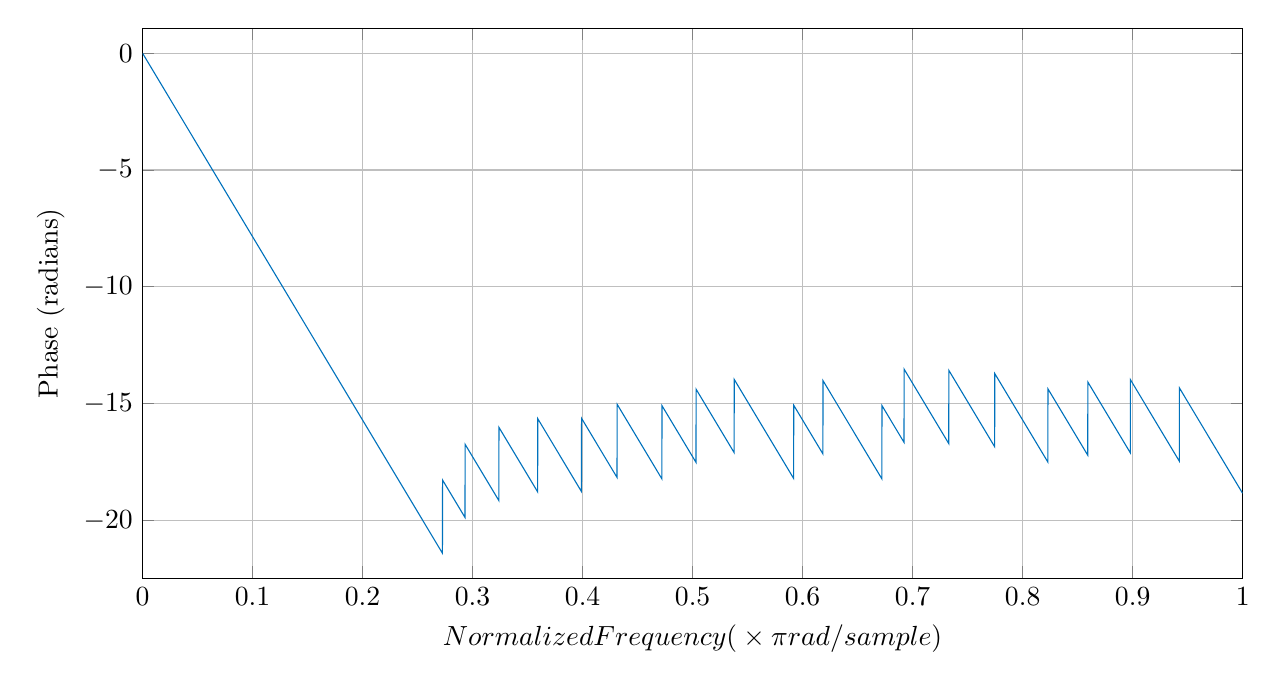
\begin{tikzpicture}

\begin{axis}[%
width=5.5in,
height=2.75in,
at={(1.281in,0.447in)},
scale only axis,
xmin=0,
xmax=0.9998779296875,
xlabel={$\text{Normalized Frequency (}\times\pi\text{ rad/sample)}$},
xmajorgrids,
ymin=-22.479050339472,
ymax=1.07043096854628,
ylabel={Phase (radians)},
ymajorgrids,
axis background/.style={fill=white},
]
\addplot [color=mycolor1,solid,forget plot]
  table[row sep=crcr]{%
0	0\\
0.0001220703125	-0.00958737992428528\\
0.000244140625	-0.0191747598485705\\
0.0003662109375	-0.0287621397728558\\
0.00048828125	-0.038349519697141\\
0.0006103515625	-0.0479368996214263\\
0.000732421875	-0.0575242795457115\\
0.0008544921875	-0.0671116594699968\\
0.0009765625	-0.076699039394282\\
0.0010986328125	-0.0862864193185673\\
0.001220703125	-0.0958737992428526\\
0.0013427734375	-0.105461179167138\\
0.00146484375	-0.115048559091423\\
0.0015869140625	-0.124635939015708\\
0.001708984375	-0.134223318939994\\
0.0018310546875	-0.143810698864279\\
0.001953125	-0.153398078788564\\
0.0020751953125	-0.162985458712849\\
0.002197265625	-0.172572838637135\\
0.0023193359375	-0.18216021856142\\
0.00244140625	-0.191747598485705\\
0.0025634765625	-0.20133497840999\\
0.002685546875	-0.210922358334276\\
0.0028076171875	-0.220509738258561\\
0.0029296875	-0.230097118182846\\
0.0030517578125	-0.239684498107131\\
0.003173828125	-0.249271878031417\\
0.0032958984375	-0.258859257955702\\
0.00341796875	-0.268446637879987\\
0.0035400390625	-0.278034017804273\\
0.003662109375	-0.287621397728558\\
0.0037841796875	-0.297208777652843\\
0.00390625	-0.306796157577128\\
0.0040283203125	-0.316383537501414\\
0.004150390625	-0.325970917425699\\
0.0042724609375	-0.335558297349984\\
0.00439453125	-0.345145677274269\\
0.0045166015625	-0.354733057198555\\
0.004638671875	-0.36432043712284\\
0.0047607421875	-0.373907817047125\\
0.0048828125	-0.38349519697141\\
0.0050048828125	-0.393082576895696\\
0.005126953125	-0.402669956819981\\
0.0052490234375	-0.412257336744266\\
0.00537109375	-0.421844716668551\\
0.0054931640625	-0.431432096592836\\
0.005615234375	-0.441019476517122\\
0.0057373046875	-0.450606856441407\\
0.005859375	-0.460194236365692\\
0.0059814453125	-0.469781616289978\\
0.006103515625	-0.479368996214263\\
0.0062255859375	-0.488956376138548\\
0.00634765625	-0.498543756062833\\
0.0064697265625	-0.508131135987119\\
0.006591796875	-0.517718515911404\\
0.0067138671875	-0.527305895835689\\
0.0068359375	-0.536893275759974\\
0.0069580078125	-0.54648065568426\\
0.007080078125	-0.556068035608545\\
0.0072021484375	-0.56565541553283\\
0.00732421875	-0.575242795457115\\
0.0074462890625	-0.584830175381401\\
0.007568359375	-0.594417555305686\\
0.0076904296875	-0.604004935229971\\
0.0078125	-0.613592315154257\\
0.0079345703125	-0.623179695078542\\
0.008056640625	-0.632767075002827\\
0.0081787109375	-0.642354454927112\\
0.00830078125	-0.651941834851398\\
0.0084228515625	-0.661529214775683\\
0.008544921875	-0.671116594699968\\
0.0086669921875	-0.680703974624253\\
0.0087890625	-0.690291354548539\\
0.0089111328125	-0.699878734472824\\
0.009033203125	-0.709466114397109\\
0.0091552734375	-0.719053494321394\\
0.00927734375	-0.72864087424568\\
0.0093994140625	-0.738228254169965\\
0.009521484375	-0.74781563409425\\
0.0096435546875	-0.757403014018535\\
0.009765625	-0.766990393942821\\
0.0098876953125	-0.776577773867106\\
0.010009765625	-0.786165153791391\\
0.0101318359375	-0.795752533715676\\
0.01025390625	-0.805339913639962\\
0.0103759765625	-0.814927293564247\\
0.010498046875	-0.824514673488532\\
0.0106201171875	-0.834102053412818\\
0.0107421875	-0.843689433337103\\
0.0108642578125	-0.853276813261388\\
0.010986328125	-0.862864193185673\\
0.0111083984375	-0.872451573109958\\
0.01123046875	-0.882038953034244\\
0.0113525390625	-0.891626332958529\\
0.011474609375	-0.901213712882814\\
0.0115966796875	-0.9108010928071\\
0.01171875	-0.920388472731385\\
0.0118408203125	-0.92997585265567\\
0.011962890625	-0.939563232579955\\
0.0120849609375	-0.94915061250424\\
0.01220703125	-0.958737992428526\\
0.0123291015625	-0.968325372352811\\
0.012451171875	-0.977912752277096\\
0.0125732421875	-0.987500132201382\\
0.0126953125	-0.997087512125667\\
0.0128173828125	-1.00667489204995\\
0.012939453125	-1.01626227197424\\
0.0130615234375	-1.02584965189852\\
0.01318359375	-1.03543703182281\\
0.0133056640625	-1.04502441174709\\
0.013427734375	-1.05461179167138\\
0.0135498046875	-1.06419917159566\\
0.013671875	-1.07378655151995\\
0.0137939453125	-1.08337393144423\\
0.013916015625	-1.09296131136852\\
0.0140380859375	-1.1025486912928\\
0.01416015625	-1.11213607121709\\
0.0142822265625	-1.12172345114137\\
0.014404296875	-1.13131083106566\\
0.0145263671875	-1.14089821098995\\
0.0146484375	-1.15048559091423\\
0.0147705078125	-1.16007297083852\\
0.014892578125	-1.1696603507628\\
0.0150146484375	-1.17924773068709\\
0.01513671875	-1.18883511061137\\
0.0152587890625	-1.19842249053566\\
0.015380859375	-1.20800987045994\\
0.0155029296875	-1.21759725038423\\
0.015625	-1.22718463030851\\
0.0157470703125	-1.2367720102328\\
0.015869140625	-1.24635939015708\\
0.0159912109375	-1.25594677008137\\
0.01611328125	-1.26553415000565\\
0.0162353515625	-1.27512152992994\\
0.016357421875	-1.28470890985422\\
0.0164794921875	-1.29429628977851\\
0.0166015625	-1.30388366970279\\
0.0167236328125	-1.31347104962708\\
0.016845703125	-1.32305842955137\\
0.0169677734375	-1.33264580947565\\
0.01708984375	-1.34223318939994\\
0.0172119140625	-1.35182056932422\\
0.017333984375	-1.36140794924851\\
0.0174560546875	-1.37099532917279\\
0.017578125	-1.38058270909708\\
0.0177001953125	-1.39017008902136\\
0.017822265625	-1.39975746894565\\
0.0179443359375	-1.40934484886993\\
0.01806640625	-1.41893222879422\\
0.0181884765625	-1.4285196087185\\
0.018310546875	-1.43810698864279\\
0.0184326171875	-1.44769436856707\\
0.0185546875	-1.45728174849136\\
0.0186767578125	-1.46686912841564\\
0.018798828125	-1.47645650833993\\
0.0189208984375	-1.48604388826421\\
0.01904296875	-1.4956312681885\\
0.0191650390625	-1.50521864811279\\
0.019287109375	-1.51480602803707\\
0.0194091796875	-1.52439340796136\\
0.01953125	-1.53398078788564\\
0.0196533203125	-1.54356816780993\\
0.019775390625	-1.55315554773421\\
0.0198974609375	-1.5627429276585\\
0.02001953125	-1.57233030758278\\
0.0201416015625	-1.58191768750707\\
0.020263671875	-1.59150506743135\\
0.0203857421875	-1.60109244735564\\
0.0205078125	-1.61067982727992\\
0.0206298828125	-1.62026720720421\\
0.020751953125	-1.62985458712849\\
0.0208740234375	-1.63944196705278\\
0.02099609375	-1.64902934697706\\
0.0211181640625	-1.65861672690135\\
0.021240234375	-1.66820410682564\\
0.0213623046875	-1.67779148674992\\
0.021484375	-1.68737886667421\\
0.0216064453125	-1.69696624659849\\
0.021728515625	-1.70655362652278\\
0.0218505859375	-1.71614100644706\\
0.02197265625	-1.72572838637135\\
0.0220947265625	-1.73531576629563\\
0.022216796875	-1.74490314621992\\
0.0223388671875	-1.7544905261442\\
0.0224609375	-1.76407790606849\\
0.0225830078125	-1.77366528599277\\
0.022705078125	-1.78325266591706\\
0.0228271484375	-1.79284004584134\\
0.02294921875	-1.80242742576563\\
0.0230712890625	-1.81201480568991\\
0.023193359375	-1.8216021856142\\
0.0233154296875	-1.83118956553848\\
0.0234375	-1.84077694546277\\
0.0235595703125	-1.85036432538705\\
0.023681640625	-1.85995170531134\\
0.0238037109375	-1.86953908523563\\
0.02392578125	-1.87912646515991\\
0.0240478515625	-1.8887138450842\\
0.024169921875	-1.89830122500848\\
0.0242919921875	-1.90788860493277\\
0.0244140625	-1.91747598485705\\
0.0245361328125	-1.92706336478134\\
0.024658203125	-1.93665074470562\\
0.0247802734375	-1.94623812462991\\
0.02490234375	-1.95582550455419\\
0.0250244140625	-1.96541288447848\\
0.025146484375	-1.97500026440276\\
0.0252685546875	-1.98458764432705\\
0.025390625	-1.99417502425133\\
0.0255126953125	-2.00376240417562\\
0.025634765625	-2.0133497840999\\
0.0257568359375	-2.02293716402419\\
0.02587890625	-2.03252454394847\\
0.0260009765625	-2.04211192387276\\
0.026123046875	-2.05169930379705\\
0.0262451171875	-2.06128668372133\\
0.0263671875	-2.07087406364562\\
0.0264892578125	-2.0804614435699\\
0.026611328125	-2.09004882349419\\
0.0267333984375	-2.09963620341847\\
0.02685546875	-2.10922358334276\\
0.0269775390625	-2.11881096326704\\
0.027099609375	-2.12839834319133\\
0.0272216796875	-2.13798572311561\\
0.02734375	-2.1475731030399\\
0.0274658203125	-2.15716048296418\\
0.027587890625	-2.16674786288847\\
0.0277099609375	-2.17633524281275\\
0.02783203125	-2.18592262273704\\
0.0279541015625	-2.19551000266132\\
0.028076171875	-2.20509738258561\\
0.0281982421875	-2.21468476250989\\
0.0283203125	-2.22427214243418\\
0.0284423828125	-2.23385952235847\\
0.028564453125	-2.24344690228275\\
0.0286865234375	-2.25303428220704\\
0.02880859375	-2.26262166213132\\
0.0289306640625	-2.27220904205561\\
0.029052734375	-2.28179642197989\\
0.0291748046875	-2.29138380190418\\
0.029296875	-2.30097118182846\\
0.0294189453125	-2.31055856175275\\
0.029541015625	-2.32014594167703\\
0.0296630859375	-2.32973332160132\\
0.02978515625	-2.3393207015256\\
0.0299072265625	-2.34890808144989\\
0.030029296875	-2.35849546137417\\
0.0301513671875	-2.36808284129846\\
0.0302734375	-2.37767022122274\\
0.0303955078125	-2.38725760114703\\
0.030517578125	-2.39684498107131\\
0.0306396484375	-2.4064323609956\\
0.03076171875	-2.41601974091988\\
0.0308837890625	-2.42560712084417\\
0.031005859375	-2.43519450076846\\
0.0311279296875	-2.44478188069274\\
0.03125	-2.45436926061703\\
0.0313720703125	-2.46395664054131\\
0.031494140625	-2.4735440204656\\
0.0316162109375	-2.48313140038988\\
0.03173828125	-2.49271878031417\\
0.0318603515625	-2.50230616023845\\
0.031982421875	-2.51189354016274\\
0.0321044921875	-2.52148092008702\\
0.0322265625	-2.53106830001131\\
0.0323486328125	-2.54065567993559\\
0.032470703125	-2.55024305985988\\
0.0325927734375	-2.55983043978416\\
0.03271484375	-2.56941781970845\\
0.0328369140625	-2.57900519963273\\
0.032958984375	-2.58859257955702\\
0.0330810546875	-2.59817995948131\\
0.033203125	-2.60776733940559\\
0.0333251953125	-2.61735471932988\\
0.033447265625	-2.62694209925416\\
0.0335693359375	-2.63652947917845\\
0.03369140625	-2.64611685910273\\
0.0338134765625	-2.65570423902702\\
0.033935546875	-2.6652916189513\\
0.0340576171875	-2.67487899887559\\
0.0341796875	-2.68446637879987\\
0.0343017578125	-2.69405375872416\\
0.034423828125	-2.70364113864844\\
0.0345458984375	-2.71322851857273\\
0.03466796875	-2.72281589849701\\
0.0347900390625	-2.7324032784213\\
0.034912109375	-2.74199065834558\\
0.0350341796875	-2.75157803826987\\
0.03515625	-2.76116541819415\\
0.0352783203125	-2.77075279811844\\
0.035400390625	-2.78034017804272\\
0.0355224609375	-2.78992755796701\\
0.03564453125	-2.7995149378913\\
0.0357666015625	-2.80910231781558\\
0.035888671875	-2.81868969773987\\
0.0360107421875	-2.82827707766415\\
0.0361328125	-2.83786445758844\\
0.0362548828125	-2.84745183751272\\
0.036376953125	-2.85703921743701\\
0.0364990234375	-2.86662659736129\\
0.03662109375	-2.87621397728558\\
0.0367431640625	-2.88580135720986\\
0.036865234375	-2.89538873713415\\
0.0369873046875	-2.90497611705843\\
0.037109375	-2.91456349698272\\
0.0372314453125	-2.924150876907\\
0.037353515625	-2.93373825683129\\
0.0374755859375	-2.94332563675557\\
0.03759765625	-2.95291301667986\\
0.0377197265625	-2.96250039660414\\
0.037841796875	-2.97208777652843\\
0.0379638671875	-2.98167515645272\\
0.0380859375	-2.991262536377\\
0.0382080078125	-3.00084991630129\\
0.038330078125	-3.01043729622557\\
0.0384521484375	-3.02002467614986\\
0.03857421875	-3.02961205607414\\
0.0386962890625	-3.03919943599843\\
0.038818359375	-3.04878681592271\\
0.0389404296875	-3.058374195847\\
0.0390625	-3.06796157577128\\
0.0391845703125	-3.07754895569557\\
0.039306640625	-3.08713633561985\\
0.0394287109375	-3.09672371554414\\
0.03955078125	-3.10631109546842\\
0.0396728515625	-3.11589847539271\\
0.039794921875	-3.12548585531699\\
0.0399169921875	-3.13507323524128\\
0.0400390625	-3.14466061516556\\
0.0401611328125	-3.15424799508985\\
0.040283203125	-3.16383537501413\\
0.0404052734375	-3.17342275493842\\
0.04052734375	-3.18301013486271\\
0.0406494140625	-3.19259751478699\\
0.040771484375	-3.20218489471128\\
0.0408935546875	-3.21177227463556\\
0.041015625	-3.22135965455985\\
0.0411376953125	-3.23094703448413\\
0.041259765625	-3.24053441440842\\
0.0413818359375	-3.2501217943327\\
0.04150390625	-3.25970917425699\\
0.0416259765625	-3.26929655418127\\
0.041748046875	-3.27888393410556\\
0.0418701171875	-3.28847131402984\\
0.0419921875	-3.29805869395413\\
0.0421142578125	-3.30764607387841\\
0.042236328125	-3.3172334538027\\
0.0423583984375	-3.32682083372698\\
0.04248046875	-3.33640821365127\\
0.0426025390625	-3.34599559357555\\
0.042724609375	-3.35558297349984\\
0.0428466796875	-3.36517035342413\\
0.04296875	-3.37475773334841\\
0.0430908203125	-3.3843451132727\\
0.043212890625	-3.39393249319698\\
0.0433349609375	-3.40351987312127\\
0.04345703125	-3.41310725304555\\
0.0435791015625	-3.42269463296984\\
0.043701171875	-3.43228201289412\\
0.0438232421875	-3.44186939281841\\
0.0439453125	-3.45145677274269\\
0.0440673828125	-3.46104415266698\\
0.044189453125	-3.47063153259126\\
0.0443115234375	-3.48021891251555\\
0.04443359375	-3.48980629243983\\
0.0445556640625	-3.49939367236412\\
0.044677734375	-3.5089810522884\\
0.0447998046875	-3.51856843221269\\
0.044921875	-3.52815581213697\\
0.0450439453125	-3.53774319206126\\
0.045166015625	-3.54733057198555\\
0.0452880859375	-3.55691795190983\\
0.04541015625	-3.56650533183412\\
0.0455322265625	-3.5760927117584\\
0.045654296875	-3.58568009168269\\
0.0457763671875	-3.59526747160697\\
0.0458984375	-3.60485485153126\\
0.0460205078125	-3.61444223145554\\
0.046142578125	-3.62402961137983\\
0.0462646484375	-3.63361699130411\\
0.04638671875	-3.6432043712284\\
0.0465087890625	-3.65279175115268\\
0.046630859375	-3.66237913107697\\
0.0467529296875	-3.67196651100125\\
0.046875	-3.68155389092554\\
0.0469970703125	-3.69114127084982\\
0.047119140625	-3.70072865077411\\
0.0472412109375	-3.71031603069839\\
0.04736328125	-3.71990341062268\\
0.0474853515625	-3.72949079054697\\
0.047607421875	-3.73907817047125\\
0.0477294921875	-3.74866555039554\\
0.0478515625	-3.75825293031982\\
0.0479736328125	-3.76784031024411\\
0.048095703125	-3.77742769016839\\
0.0482177734375	-3.78701507009268\\
0.04833984375	-3.79660245001696\\
0.0484619140625	-3.80618982994125\\
0.048583984375	-3.81577720986553\\
0.0487060546875	-3.82536458978982\\
0.048828125	-3.8349519697141\\
0.0489501953125	-3.84453934963839\\
0.049072265625	-3.85412672956267\\
0.0491943359375	-3.86371410948696\\
0.04931640625	-3.87330148941124\\
0.0494384765625	-3.88288886933553\\
0.049560546875	-3.89247624925981\\
0.0496826171875	-3.9020636291841\\
0.0498046875	-3.91165100910839\\
0.0499267578125	-3.92123838903267\\
0.050048828125	-3.93082576895696\\
0.0501708984375	-3.94041314888124\\
0.05029296875	-3.95000052880553\\
0.0504150390625	-3.95958790872981\\
0.050537109375	-3.9691752886541\\
0.0506591796875	-3.97876266857838\\
0.05078125	-3.98835004850267\\
0.0509033203125	-3.99793742842695\\
0.051025390625	-4.00752480835124\\
0.0511474609375	-4.01711218827552\\
0.05126953125	-4.02669956819981\\
0.0513916015625	-4.03628694812409\\
0.051513671875	-4.04587432804838\\
0.0516357421875	-4.05546170797266\\
0.0517578125	-4.06504908789695\\
0.0518798828125	-4.07463646782123\\
0.052001953125	-4.08422384774552\\
0.0521240234375	-4.09381122766981\\
0.05224609375	-4.10339860759409\\
0.0523681640625	-4.11298598751837\\
0.052490234375	-4.12257336744266\\
0.0526123046875	-4.13216074736695\\
0.052734375	-4.14174812729123\\
0.0528564453125	-4.15133550721552\\
0.052978515625	-4.1609228871398\\
0.0531005859375	-4.17051026706409\\
0.05322265625	-4.18009764698837\\
0.0533447265625	-4.18968502691266\\
0.053466796875	-4.19927240683694\\
0.0535888671875	-4.20885978676123\\
0.0537109375	-4.21844716668551\\
0.0538330078125	-4.2280345466098\\
0.053955078125	-4.23762192653408\\
0.0540771484375	-4.24720930645837\\
0.05419921875	-4.25679668638265\\
0.0543212890625	-4.26638406630694\\
0.054443359375	-4.27597144623122\\
0.0545654296875	-4.28555882615551\\
0.0546875	-4.29514620607979\\
0.0548095703125	-4.30473358600408\\
0.054931640625	-4.31432096592837\\
0.0550537109375	-4.32390834585265\\
0.05517578125	-4.33349572577694\\
0.0552978515625	-4.34308310570122\\
0.055419921875	-4.35267048562551\\
0.0555419921875	-4.36225786554979\\
0.0556640625	-4.37184524547408\\
0.0557861328125	-4.38143262539836\\
0.055908203125	-4.39102000532265\\
0.0560302734375	-4.40060738524693\\
0.05615234375	-4.41019476517122\\
0.0562744140625	-4.4197821450955\\
0.056396484375	-4.42936952501979\\
0.0565185546875	-4.43895690494407\\
0.056640625	-4.44854428486836\\
0.0567626953125	-4.45813166479264\\
0.056884765625	-4.46771904471693\\
0.0570068359375	-4.47730642464122\\
0.05712890625	-4.4868938045655\\
0.0572509765625	-4.49648118448979\\
0.057373046875	-4.50606856441407\\
0.0574951171875	-4.51565594433836\\
0.0576171875	-4.52524332426264\\
0.0577392578125	-4.53483070418693\\
0.057861328125	-4.54441808411121\\
0.0579833984375	-4.5540054640355\\
0.05810546875	-4.56359284395978\\
0.0582275390625	-4.57318022388407\\
0.058349609375	-4.58276760380835\\
0.0584716796875	-4.59235498373264\\
0.05859375	-4.60194236365692\\
0.0587158203125	-4.61152974358121\\
0.058837890625	-4.62111712350549\\
0.0589599609375	-4.63070450342978\\
0.05908203125	-4.64029188335406\\
0.0592041015625	-4.64987926327835\\
0.059326171875	-4.65946664320263\\
0.0594482421875	-4.66905402312692\\
0.0595703125	-4.67864140305121\\
0.0596923828125	-4.68822878297549\\
0.059814453125	-4.69781616289978\\
0.0599365234375	-4.70740354282406\\
0.06005859375	-4.71699092274835\\
0.0601806640625	-4.72657830267263\\
0.060302734375	-4.73616568259692\\
0.0604248046875	-4.7457530625212\\
0.060546875	-4.75534044244549\\
0.0606689453125	-4.76492782236977\\
0.060791015625	-4.77451520229406\\
0.0609130859375	-4.78410258221834\\
0.06103515625	-4.79368996214263\\
0.0611572265625	-4.80327734206691\\
0.061279296875	-4.8128647219912\\
0.0614013671875	-4.82245210191548\\
0.0615234375	-4.83203948183977\\
0.0616455078125	-4.84162686176405\\
0.061767578125	-4.85121424168834\\
0.0618896484375	-4.86080162161262\\
0.06201171875	-4.87038900153691\\
0.0621337890625	-4.8799763814612\\
0.062255859375	-4.88956376138548\\
0.0623779296875	-4.89915114130977\\
0.0625	-4.90873852123405\\
0.0626220703125	-4.91832590115834\\
0.062744140625	-4.92791328108262\\
0.0628662109375	-4.93750066100691\\
0.06298828125	-4.94708804093119\\
0.0631103515625	-4.95667542085548\\
0.063232421875	-4.96626280077976\\
0.0633544921875	-4.97585018070405\\
0.0634765625	-4.98543756062833\\
0.0635986328125	-4.99502494055262\\
0.063720703125	-5.0046123204769\\
0.0638427734375	-5.01419970040119\\
0.06396484375	-5.02378708032547\\
0.0640869140625	-5.03337446024976\\
0.064208984375	-5.04296184017405\\
0.0643310546875	-5.05254922009833\\
0.064453125	-5.06213660002262\\
0.0645751953125	-5.0717239799469\\
0.064697265625	-5.08131135987119\\
0.0648193359375	-5.09089873979547\\
0.06494140625	-5.10048611971976\\
0.0650634765625	-5.11007349964404\\
0.065185546875	-5.11966087956833\\
0.0653076171875	-5.12924825949261\\
0.0654296875	-5.1388356394169\\
0.0655517578125	-5.14842301934118\\
0.065673828125	-5.15801039926547\\
0.0657958984375	-5.16759777918975\\
0.06591796875	-5.17718515911404\\
0.0660400390625	-5.18677253903832\\
0.066162109375	-5.19635991896261\\
0.0662841796875	-5.20594729888689\\
0.06640625	-5.21553467881118\\
0.0665283203125	-5.22512205873547\\
0.066650390625	-5.23470943865975\\
0.0667724609375	-5.24429681858404\\
0.06689453125	-5.25388419850832\\
0.0670166015625	-5.26347157843261\\
0.067138671875	-5.27305895835689\\
0.0672607421875	-5.28264633828118\\
0.0673828125	-5.29223371820546\\
0.0675048828125	-5.30182109812975\\
0.067626953125	-5.31140847805403\\
0.0677490234375	-5.32099585797832\\
0.06787109375	-5.3305832379026\\
0.0679931640625	-5.34017061782689\\
0.068115234375	-5.34975799775117\\
0.0682373046875	-5.35934537767546\\
0.068359375	-5.36893275759974\\
0.0684814453125	-5.37852013752403\\
0.068603515625	-5.38810751744832\\
0.0687255859375	-5.3976948973726\\
0.06884765625	-5.40728227729689\\
0.0689697265625	-5.41686965722117\\
0.069091796875	-5.42645703714546\\
0.0692138671875	-5.43604441706974\\
0.0693359375	-5.44563179699403\\
0.0694580078125	-5.45521917691831\\
0.069580078125	-5.4648065568426\\
0.0697021484375	-5.47439393676688\\
0.06982421875	-5.48398131669117\\
0.0699462890625	-5.49356869661545\\
0.070068359375	-5.50315607653974\\
0.0701904296875	-5.51274345646402\\
0.0703125	-5.52233083638831\\
0.0704345703125	-5.53191821631259\\
0.070556640625	-5.54150559623688\\
0.0706787109375	-5.55109297616116\\
0.07080078125	-5.56068035608545\\
0.0709228515625	-5.57026773600973\\
0.071044921875	-5.57985511593402\\
0.0711669921875	-5.5894424958583\\
0.0712890625	-5.59902987578259\\
0.0714111328125	-5.60861725570688\\
0.071533203125	-5.61820463563116\\
0.0716552734375	-5.62779201555545\\
0.07177734375	-5.63737939547973\\
0.0718994140625	-5.64696677540402\\
0.072021484375	-5.6565541553283\\
0.0721435546875	-5.66614153525259\\
0.072265625	-5.67572891517687\\
0.0723876953125	-5.68531629510116\\
0.072509765625	-5.69490367502544\\
0.0726318359375	-5.70449105494973\\
0.07275390625	-5.71407843487401\\
0.0728759765625	-5.7236658147983\\
0.072998046875	-5.73325319472258\\
0.0731201171875	-5.74284057464687\\
0.0732421875	-5.75242795457115\\
0.0733642578125	-5.76201533449544\\
0.073486328125	-5.77160271441972\\
0.0736083984375	-5.78119009434401\\
0.07373046875	-5.7907774742683\\
0.0738525390625	-5.80036485419258\\
0.073974609375	-5.80995223411687\\
0.0740966796875	-5.81953961404115\\
0.07421875	-5.82912699396544\\
0.0743408203125	-5.83871437388972\\
0.074462890625	-5.84830175381401\\
0.0745849609375	-5.85788913373829\\
0.07470703125	-5.86747651366258\\
0.0748291015625	-5.87706389358686\\
0.074951171875	-5.88665127351115\\
0.0750732421875	-5.89623865343543\\
0.0751953125	-5.90582603335972\\
0.0753173828125	-5.915413413284\\
0.075439453125	-5.92500079320829\\
0.0755615234375	-5.93458817313257\\
0.07568359375	-5.94417555305686\\
0.0758056640625	-5.95376293298115\\
0.075927734375	-5.96335031290543\\
0.0760498046875	-5.97293769282972\\
0.076171875	-5.982525072754\\
0.0762939453125	-5.99211245267829\\
0.076416015625	-6.00169983260257\\
0.0765380859375	-6.01128721252686\\
0.07666015625	-6.02087459245114\\
0.0767822265625	-6.03046197237543\\
0.076904296875	-6.04004935229971\\
0.0770263671875	-6.049636732224\\
0.0771484375	-6.05922411214828\\
0.0772705078125	-6.06881149207257\\
0.077392578125	-6.07839887199685\\
0.0775146484375	-6.08798625192114\\
0.07763671875	-6.09757363184542\\
0.0777587890625	-6.10716101176971\\
0.077880859375	-6.11674839169399\\
0.0780029296875	-6.12633577161828\\
0.078125	-6.13592315154256\\
0.0782470703125	-6.14551053146685\\
0.078369140625	-6.15509791139114\\
0.0784912109375	-6.16468529131542\\
0.07861328125	-6.17427267123971\\
0.0787353515625	-6.18386005116399\\
0.078857421875	-6.19344743108828\\
0.0789794921875	-6.20303481101256\\
0.0791015625	-6.21262219093685\\
0.0792236328125	-6.22220957086113\\
0.079345703125	-6.23179695078542\\
0.0794677734375	-6.2413843307097\\
0.07958984375	-6.25097171063399\\
0.0797119140625	-6.26055909055827\\
0.079833984375	-6.27014647048256\\
0.0799560546875	-6.27973385040684\\
0.080078125	-6.28932123033113\\
0.0802001953125	-6.29890861025541\\
0.080322265625	-6.3084959901797\\
0.0804443359375	-6.31808337010398\\
0.08056640625	-6.32767075002827\\
0.0806884765625	-6.33725812995255\\
0.080810546875	-6.34684550987684\\
0.0809326171875	-6.35643288980113\\
0.0810546875	-6.36602026972541\\
0.0811767578125	-6.3756076496497\\
0.081298828125	-6.38519502957398\\
0.0814208984375	-6.39478240949827\\
0.08154296875	-6.40436978942255\\
0.0816650390625	-6.41395716934684\\
0.081787109375	-6.42354454927112\\
0.0819091796875	-6.43313192919541\\
0.08203125	-6.44271930911969\\
0.0821533203125	-6.45230668904398\\
0.082275390625	-6.46189406896826\\
0.0823974609375	-6.47148144889255\\
0.08251953125	-6.48106882881683\\
0.0826416015625	-6.49065620874112\\
0.082763671875	-6.5002435886654\\
0.0828857421875	-6.50983096858969\\
0.0830078125	-6.51941834851397\\
0.0831298828125	-6.52900572843826\\
0.083251953125	-6.53859310836255\\
0.0833740234375	-6.54818048828683\\
0.08349609375	-6.55776786821112\\
0.0836181640625	-6.5673552481354\\
0.083740234375	-6.57694262805969\\
0.0838623046875	-6.58653000798397\\
0.083984375	-6.59611738790826\\
0.0841064453125	-6.60570476783254\\
0.084228515625	-6.61529214775683\\
0.0843505859375	-6.62487952768111\\
0.08447265625	-6.6344669076054\\
0.0845947265625	-6.64405428752968\\
0.084716796875	-6.65364166745397\\
0.0848388671875	-6.66322904737825\\
0.0849609375	-6.67281642730254\\
0.0850830078125	-6.68240380722682\\
0.085205078125	-6.69199118715111\\
0.0853271484375	-6.7015785670754\\
0.08544921875	-6.71116594699968\\
0.0855712890625	-6.72075332692397\\
0.085693359375	-6.73034070684825\\
0.0858154296875	-6.73992808677254\\
0.0859375	-6.74951546669682\\
0.0860595703125	-6.75910284662111\\
0.086181640625	-6.76869022654539\\
0.0863037109375	-6.77827760646968\\
0.08642578125	-6.78786498639396\\
0.0865478515625	-6.79745236631825\\
0.086669921875	-6.80703974624253\\
0.0867919921875	-6.81662712616682\\
0.0869140625	-6.8262145060911\\
0.0870361328125	-6.83580188601539\\
0.087158203125	-6.84538926593967\\
0.0872802734375	-6.85497664586396\\
0.08740234375	-6.86456402578824\\
0.0875244140625	-6.87415140571253\\
0.087646484375	-6.88373878563681\\
0.0877685546875	-6.8933261655611\\
0.087890625	-6.90291354548539\\
0.0880126953125	-6.91250092540967\\
0.088134765625	-6.92208830533396\\
0.0882568359375	-6.93167568525824\\
0.08837890625	-6.94126306518253\\
0.0885009765625	-6.95085044510681\\
0.088623046875	-6.9604378250311\\
0.0887451171875	-6.97002520495538\\
0.0888671875	-6.97961258487967\\
0.0889892578125	-6.98919996480395\\
0.089111328125	-6.99878734472824\\
0.0892333984375	-7.00837472465252\\
0.08935546875	-7.01796210457681\\
0.0894775390625	-7.02754948450109\\
0.089599609375	-7.03713686442538\\
0.0897216796875	-7.04672424434966\\
0.08984375	-7.05631162427395\\
0.0899658203125	-7.06589900419823\\
0.090087890625	-7.07548638412252\\
0.0902099609375	-7.0850737640468\\
0.09033203125	-7.09466114397109\\
0.0904541015625	-7.10424852389538\\
0.090576171875	-7.11383590381966\\
0.0906982421875	-7.12342328374395\\
0.0908203125	-7.13301066366823\\
0.0909423828125	-7.14259804359252\\
0.091064453125	-7.1521854235168\\
0.0911865234375	-7.16177280344109\\
0.09130859375	-7.17136018336537\\
0.0914306640625	-7.18094756328966\\
0.091552734375	-7.19053494321394\\
0.0916748046875	-7.20012232313823\\
0.091796875	-7.20970970306251\\
0.0919189453125	-7.2192970829868\\
0.092041015625	-7.22888446291108\\
0.0921630859375	-7.23847184283537\\
0.09228515625	-7.24805922275965\\
0.0924072265625	-7.25764660268394\\
0.092529296875	-7.26723398260823\\
0.0926513671875	-7.27682136253251\\
0.0927734375	-7.2864087424568\\
0.0928955078125	-7.29599612238108\\
0.093017578125	-7.30558350230537\\
0.0931396484375	-7.31517088222965\\
0.09326171875	-7.32475826215394\\
0.0933837890625	-7.33434564207822\\
0.093505859375	-7.34393302200251\\
0.0936279296875	-7.35352040192679\\
0.09375	-7.36310778185108\\
0.0938720703125	-7.37269516177536\\
0.093994140625	-7.38228254169965\\
0.0941162109375	-7.39186992162393\\
0.09423828125	-7.40145730154822\\
0.0943603515625	-7.4110446814725\\
0.094482421875	-7.42063206139679\\
0.0946044921875	-7.43021944132107\\
0.0947265625	-7.43980682124536\\
0.0948486328125	-7.44939420116965\\
0.094970703125	-7.45898158109393\\
0.0950927734375	-7.46856896101822\\
0.09521484375	-7.4781563409425\\
0.0953369140625	-7.48774372086679\\
0.095458984375	-7.49733110079107\\
0.0955810546875	-7.50691848071536\\
0.095703125	-7.51650586063964\\
0.0958251953125	-7.52609324056393\\
0.095947265625	-7.53568062048821\\
0.0960693359375	-7.5452680004125\\
0.09619140625	-7.55485538033678\\
0.0963134765625	-7.56444276026107\\
0.096435546875	-7.57403014018535\\
0.0965576171875	-7.58361752010964\\
0.0966796875	-7.59320490003392\\
0.0968017578125	-7.60279227995821\\
0.096923828125	-7.61237965988249\\
0.0970458984375	-7.62196703980678\\
0.09716796875	-7.63155441973106\\
0.0972900390625	-7.64114179965535\\
0.097412109375	-7.65072917957963\\
0.0975341796875	-7.66031655950392\\
0.09765625	-7.66990393942821\\
0.0977783203125	-7.67949131935249\\
0.097900390625	-7.68907869927678\\
0.0980224609375	-7.69866607920106\\
0.09814453125	-7.70825345912535\\
0.0982666015625	-7.71784083904963\\
0.098388671875	-7.72742821897392\\
0.0985107421875	-7.7370155988982\\
0.0986328125	-7.74660297882249\\
0.0987548828125	-7.75619035874677\\
0.098876953125	-7.76577773867106\\
0.0989990234375	-7.77536511859534\\
0.09912109375	-7.78495249851963\\
0.0992431640625	-7.79453987844391\\
0.099365234375	-7.8041272583682\\
0.0994873046875	-7.81371463829248\\
0.099609375	-7.82330201821677\\
0.0997314453125	-7.83288939814106\\
0.099853515625	-7.84247677806534\\
0.0999755859375	-7.85206415798963\\
0.10009765625	-7.86165153791391\\
0.1002197265625	-7.8712389178382\\
0.100341796875	-7.88082629776248\\
0.1004638671875	-7.89041367768677\\
0.1005859375	-7.90000105761105\\
0.1007080078125	-7.90958843753534\\
0.100830078125	-7.91917581745962\\
0.1009521484375	-7.92876319738391\\
0.10107421875	-7.93835057730819\\
0.1011962890625	-7.94793795723248\\
0.101318359375	-7.95752533715676\\
0.1014404296875	-7.96711271708105\\
0.1015625	-7.97670009700533\\
0.1016845703125	-7.98628747692962\\
0.101806640625	-7.9958748568539\\
0.1019287109375	-8.00546223677819\\
0.10205078125	-8.01504961670248\\
0.1021728515625	-8.02463699662676\\
0.102294921875	-8.03422437655105\\
0.1024169921875	-8.04381175647533\\
0.1025390625	-8.05339913639962\\
0.1026611328125	-8.0629865163239\\
0.102783203125	-8.07257389624819\\
0.1029052734375	-8.08216127617247\\
0.10302734375	-8.09174865609676\\
0.1031494140625	-8.10133603602104\\
0.103271484375	-8.11092341594533\\
0.1033935546875	-8.12051079586961\\
0.103515625	-8.1300981757939\\
0.1036376953125	-8.13968555571818\\
0.103759765625	-8.14927293564247\\
0.1038818359375	-8.15886031556675\\
0.10400390625	-8.16844769549104\\
0.1041259765625	-8.17803507541533\\
0.104248046875	-8.18762245533961\\
0.1043701171875	-8.19720983526389\\
0.1044921875	-8.20679721518818\\
0.1046142578125	-8.21638459511247\\
0.104736328125	-8.22597197503675\\
0.1048583984375	-8.23555935496104\\
0.10498046875	-8.24514673488532\\
0.1051025390625	-8.25473411480961\\
0.105224609375	-8.26432149473389\\
0.1053466796875	-8.27390887465818\\
0.10546875	-8.28349625458246\\
0.1055908203125	-8.29308363450675\\
0.105712890625	-8.30267101443103\\
0.1058349609375	-8.31225839435532\\
0.10595703125	-8.3218457742796\\
0.1060791015625	-8.33143315420389\\
0.106201171875	-8.34102053412817\\
0.1063232421875	-8.35060791405246\\
0.1064453125	-8.36019529397674\\
0.1065673828125	-8.36978267390103\\
0.106689453125	-8.37937005382532\\
0.1068115234375	-8.3889574337496\\
0.10693359375	-8.39854481367388\\
0.1070556640625	-8.40813219359817\\
0.107177734375	-8.41771957352246\\
0.1072998046875	-8.42730695344674\\
0.107421875	-8.43689433337103\\
0.1075439453125	-8.44648171329531\\
0.107666015625	-8.4560690932196\\
0.1077880859375	-8.46565647314388\\
0.10791015625	-8.47524385306817\\
0.1080322265625	-8.48483123299245\\
0.108154296875	-8.49441861291674\\
0.1082763671875	-8.50400599284102\\
0.1083984375	-8.51359337276531\\
0.1085205078125	-8.52318075268959\\
0.108642578125	-8.53276813261388\\
0.1087646484375	-8.54235551253817\\
0.10888671875	-8.55194289246245\\
0.1090087890625	-8.56153027238673\\
0.109130859375	-8.57111765231102\\
0.1092529296875	-8.5807050322353\\
0.109375	-8.59029241215959\\
0.1094970703125	-8.59987979208388\\
0.109619140625	-8.60946717200816\\
0.1097412109375	-8.61905455193245\\
0.10986328125	-8.62864193185673\\
0.1099853515625	-8.63822931178102\\
0.110107421875	-8.6478166917053\\
0.1102294921875	-8.65740407162959\\
0.1103515625	-8.66699145155387\\
0.1104736328125	-8.67657883147816\\
0.110595703125	-8.68616621140244\\
0.1107177734375	-8.69575359132673\\
0.11083984375	-8.70534097125101\\
0.1109619140625	-8.7149283511753\\
0.111083984375	-8.72451573109958\\
0.1112060546875	-8.73410311102387\\
0.111328125	-8.74369049094815\\
0.1114501953125	-8.75327787087244\\
0.111572265625	-8.76286525079673\\
0.1116943359375	-8.77245263072101\\
0.11181640625	-8.7820400106453\\
0.1119384765625	-8.79162739056958\\
0.112060546875	-8.80121477049387\\
0.1121826171875	-8.81080215041815\\
0.1123046875	-8.82038953034244\\
0.1124267578125	-8.82997691026672\\
0.112548828125	-8.83956429019101\\
0.1126708984375	-8.84915167011529\\
0.11279296875	-8.85873905003958\\
0.1129150390625	-8.86832642996386\\
0.113037109375	-8.87791380988815\\
0.1131591796875	-8.88750118981243\\
0.11328125	-8.89708856973672\\
0.1134033203125	-8.906675949661\\
0.113525390625	-8.91626332958529\\
0.1136474609375	-8.92585070950958\\
0.11376953125	-8.93543808943386\\
0.1138916015625	-8.94502546935815\\
0.114013671875	-8.95461284928243\\
0.1141357421875	-8.96420022920672\\
0.1142578125	-8.973787609131\\
0.1143798828125	-8.98337498905529\\
0.114501953125	-8.99296236897957\\
0.1146240234375	-9.00254974890386\\
0.11474609375	-9.01213712882814\\
0.1148681640625	-9.02172450875243\\
0.114990234375	-9.03131188867671\\
0.1151123046875	-9.040899268601\\
0.115234375	-9.05048664852528\\
0.1153564453125	-9.06007402844957\\
0.115478515625	-9.06966140837385\\
0.1156005859375	-9.07924878829814\\
0.11572265625	-9.08883616822243\\
0.1158447265625	-9.09842354814671\\
0.115966796875	-9.10801092807099\\
0.1160888671875	-9.11759830799528\\
0.1162109375	-9.12718568791957\\
0.1163330078125	-9.13677306784385\\
0.116455078125	-9.14636044776814\\
0.1165771484375	-9.15594782769242\\
0.11669921875	-9.16553520761671\\
0.1168212890625	-9.17512258754099\\
0.116943359375	-9.18470996746528\\
0.1170654296875	-9.19429734738956\\
0.1171875	-9.20388472731385\\
0.1173095703125	-9.21347210723813\\
0.117431640625	-9.22305948716242\\
0.1175537109375	-9.2326468670867\\
0.11767578125	-9.24223424701099\\
0.1177978515625	-9.25182162693527\\
0.117919921875	-9.26140900685956\\
0.1180419921875	-9.27099638678384\\
0.1181640625	-9.28058376670813\\
0.1182861328125	-9.29017114663241\\
0.118408203125	-9.2997585265567\\
0.1185302734375	-9.30934590648098\\
0.11865234375	-9.31893328640527\\
0.1187744140625	-9.32852066632956\\
0.118896484375	-9.33810804625384\\
0.1190185546875	-9.34769542617813\\
0.119140625	-9.35728280610241\\
0.1192626953125	-9.3668701860267\\
0.119384765625	-9.37645756595098\\
0.1195068359375	-9.38604494587527\\
0.11962890625	-9.39563232579955\\
0.1197509765625	-9.40521970572384\\
0.119873046875	-9.41480708564812\\
0.1199951171875	-9.42439446557241\\
0.1201171875	-9.43398184549669\\
0.1202392578125	-9.44356922542098\\
0.120361328125	-9.45315660534526\\
0.1204833984375	-9.46274398526955\\
0.12060546875	-9.47233136519383\\
0.1207275390625	-9.48191874511812\\
0.120849609375	-9.4915061250424\\
0.1209716796875	-9.50109350496669\\
0.12109375	-9.51068088489098\\
0.1212158203125	-9.52026826481526\\
0.121337890625	-9.52985564473954\\
0.1214599609375	-9.53944302466383\\
0.12158203125	-9.54903040458812\\
0.1217041015625	-9.5586177845124\\
0.121826171875	-9.56820516443669\\
0.1219482421875	-9.57779254436097\\
0.1220703125	-9.58737992428526\\
0.1221923828125	-9.59696730420954\\
0.122314453125	-9.60655468413383\\
0.1224365234375	-9.61614206405811\\
0.12255859375	-9.6257294439824\\
0.1226806640625	-9.63531682390668\\
0.122802734375	-9.64490420383097\\
0.1229248046875	-9.65449158375525\\
0.123046875	-9.66407896367954\\
0.1231689453125	-9.67366634360382\\
0.123291015625	-9.68325372352811\\
0.1234130859375	-9.69284110345239\\
0.12353515625	-9.70242848337668\\
0.1236572265625	-9.71201586330097\\
0.123779296875	-9.72160324322525\\
0.1239013671875	-9.73119062314954\\
0.1240234375	-9.74077800307382\\
0.1241455078125	-9.75036538299811\\
0.124267578125	-9.75995276292239\\
0.1243896484375	-9.76954014284668\\
0.12451171875	-9.77912752277096\\
0.1246337890625	-9.78871490269525\\
0.124755859375	-9.79830228261953\\
0.1248779296875	-9.80788966254382\\
0.125	-9.8174770424681\\
0.1251220703125	-9.82706442239239\\
0.125244140625	-9.83665180231667\\
0.1253662109375	-9.84623918224096\\
0.12548828125	-9.85582656216524\\
0.1256103515625	-9.86541394208953\\
0.125732421875	-9.87500132201382\\
0.1258544921875	-9.8845887019381\\
0.1259765625	-9.89417608186239\\
0.1260986328125	-9.90376346178667\\
0.126220703125	-9.91335084171096\\
0.1263427734375	-9.92293822163524\\
0.12646484375	-9.93252560155953\\
0.1265869140625	-9.94211298148381\\
0.126708984375	-9.9517003614081\\
0.1268310546875	-9.96128774133238\\
0.126953125	-9.97087512125667\\
0.1270751953125	-9.98046250118095\\
0.127197265625	-9.99004988110524\\
0.1273193359375	-9.99963726102952\\
0.12744140625	-10.0092246409538\\
0.1275634765625	-10.0188120208781\\
0.127685546875	-10.0283994008024\\
0.1278076171875	-10.0379867807267\\
0.1279296875	-10.0475741606509\\
0.1280517578125	-10.0571615405752\\
0.128173828125	-10.0667489204995\\
0.1282958984375	-10.0763363004238\\
0.12841796875	-10.0859236803481\\
0.1285400390625	-10.0955110602724\\
0.128662109375	-10.1050984401967\\
0.1287841796875	-10.1146858201209\\
0.12890625	-10.1242732000452\\
0.1290283203125	-10.1338605799695\\
0.129150390625	-10.1434479598938\\
0.1292724609375	-10.1530353398181\\
0.12939453125	-10.1626227197424\\
0.1295166015625	-10.1722100996667\\
0.129638671875	-10.1817974795909\\
0.1297607421875	-10.1913848595152\\
0.1298828125	-10.2009722394395\\
0.1300048828125	-10.2105596193638\\
0.130126953125	-10.2201469992881\\
0.1302490234375	-10.2297343792124\\
0.13037109375	-10.2393217591367\\
0.1304931640625	-10.2489091390609\\
0.130615234375	-10.2584965189852\\
0.1307373046875	-10.2680838989095\\
0.130859375	-10.2776712788338\\
0.1309814453125	-10.2872586587581\\
0.131103515625	-10.2968460386824\\
0.1312255859375	-10.3064334186067\\
0.13134765625	-10.3160207985309\\
0.1314697265625	-10.3256081784552\\
0.131591796875	-10.3351955583795\\
0.1317138671875	-10.3447829383038\\
0.1318359375	-10.3543703182281\\
0.1319580078125	-10.3639576981524\\
0.132080078125	-10.3735450780766\\
0.1322021484375	-10.3831324580009\\
0.13232421875	-10.3927198379252\\
0.1324462890625	-10.4023072178495\\
0.132568359375	-10.4118945977738\\
0.1326904296875	-10.4214819776981\\
0.1328125	-10.4310693576224\\
0.1329345703125	-10.4406567375466\\
0.133056640625	-10.4502441174709\\
0.1331787109375	-10.4598314973952\\
0.13330078125	-10.4694188773195\\
0.1334228515625	-10.4790062572438\\
0.133544921875	-10.4885936371681\\
0.1336669921875	-10.4981810170924\\
0.1337890625	-10.5077683970166\\
0.1339111328125	-10.5173557769409\\
0.134033203125	-10.5269431568652\\
0.1341552734375	-10.5365305367895\\
0.13427734375	-10.5461179167138\\
0.1343994140625	-10.5557052966381\\
0.134521484375	-10.5652926765624\\
0.1346435546875	-10.5748800564866\\
0.134765625	-10.5844674364109\\
0.1348876953125	-10.5940548163352\\
0.135009765625	-10.6036421962595\\
0.1351318359375	-10.6132295761838\\
0.13525390625	-10.6228169561081\\
0.1353759765625	-10.6324043360324\\
0.135498046875	-10.6419917159566\\
0.1356201171875	-10.6515790958809\\
0.1357421875	-10.6611664758052\\
0.1358642578125	-10.6707538557295\\
0.135986328125	-10.6803412356538\\
0.1361083984375	-10.6899286155781\\
0.13623046875	-10.6995159955023\\
0.1363525390625	-10.7091033754266\\
0.136474609375	-10.7186907553509\\
0.1365966796875	-10.7282781352752\\
0.13671875	-10.7378655151995\\
0.1368408203125	-10.7474528951238\\
0.136962890625	-10.7570402750481\\
0.1370849609375	-10.7666276549723\\
0.13720703125	-10.7762150348966\\
0.1373291015625	-10.7858024148209\\
0.137451171875	-10.7953897947452\\
0.1375732421875	-10.8049771746695\\
0.1376953125	-10.8145645545938\\
0.1378173828125	-10.8241519345181\\
0.137939453125	-10.8337393144423\\
0.1380615234375	-10.8433266943666\\
0.13818359375	-10.8529140742909\\
0.1383056640625	-10.8625014542152\\
0.138427734375	-10.8720888341395\\
0.1385498046875	-10.8816762140638\\
0.138671875	-10.8912635939881\\
0.1387939453125	-10.9008509739123\\
0.138916015625	-10.9104383538366\\
0.1390380859375	-10.9200257337609\\
0.13916015625	-10.9296131136852\\
0.1392822265625	-10.9392004936095\\
0.139404296875	-10.9487878735338\\
0.1395263671875	-10.958375253458\\
0.1396484375	-10.9679626333823\\
0.1397705078125	-10.9775500133066\\
0.139892578125	-10.9871373932309\\
0.1400146484375	-10.9967247731552\\
0.14013671875	-11.0063121530795\\
0.1402587890625	-11.0158995330038\\
0.140380859375	-11.025486912928\\
0.1405029296875	-11.0350742928523\\
0.140625	-11.0446616727766\\
0.1407470703125	-11.0542490527009\\
0.140869140625	-11.0638364326252\\
0.1409912109375	-11.0734238125495\\
0.14111328125	-11.0830111924738\\
0.1412353515625	-11.092598572398\\
0.141357421875	-11.1021859523223\\
0.1414794921875	-11.1117733322466\\
0.1416015625	-11.1213607121709\\
0.1417236328125	-11.1309480920952\\
0.141845703125	-11.1405354720195\\
0.1419677734375	-11.1501228519438\\
0.14208984375	-11.159710231868\\
0.1422119140625	-11.1692976117923\\
0.142333984375	-11.1788849917166\\
0.1424560546875	-11.1884723716409\\
0.142578125	-11.1980597515652\\
0.1427001953125	-11.2076471314895\\
0.142822265625	-11.2172345114138\\
0.1429443359375	-11.226821891338\\
0.14306640625	-11.2364092712623\\
0.1431884765625	-11.2459966511866\\
0.143310546875	-11.2555840311109\\
0.1434326171875	-11.2651714110352\\
0.1435546875	-11.2747587909595\\
0.1436767578125	-11.2843461708837\\
0.143798828125	-11.293933550808\\
0.1439208984375	-11.3035209307323\\
0.14404296875	-11.3131083106566\\
0.1441650390625	-11.3226956905809\\
0.144287109375	-11.3322830705052\\
0.1444091796875	-11.3418704504295\\
0.14453125	-11.3514578303537\\
0.1446533203125	-11.361045210278\\
0.144775390625	-11.3706325902023\\
0.1448974609375	-11.3802199701266\\
0.14501953125	-11.3898073500509\\
0.1451416015625	-11.3993947299752\\
0.145263671875	-11.4089821098995\\
0.1453857421875	-11.4185694898237\\
0.1455078125	-11.428156869748\\
0.1456298828125	-11.4377442496723\\
0.145751953125	-11.4473316295966\\
0.1458740234375	-11.4569190095209\\
0.14599609375	-11.4665063894452\\
0.1461181640625	-11.4760937693695\\
0.146240234375	-11.4856811492937\\
0.1463623046875	-11.495268529218\\
0.146484375	-11.5048559091423\\
0.1466064453125	-11.5144432890666\\
0.146728515625	-11.5240306689909\\
0.1468505859375	-11.5336180489152\\
0.14697265625	-11.5432054288395\\
0.1470947265625	-11.5527928087637\\
0.147216796875	-11.562380188688\\
0.1473388671875	-11.5719675686123\\
0.1474609375	-11.5815549485366\\
0.1475830078125	-11.5911423284609\\
0.147705078125	-11.6007297083852\\
0.1478271484375	-11.6103170883094\\
0.14794921875	-11.6199044682337\\
0.1480712890625	-11.629491848158\\
0.148193359375	-11.6390792280823\\
0.1483154296875	-11.6486666080066\\
0.1484375	-11.6582539879309\\
0.1485595703125	-11.6678413678552\\
0.148681640625	-11.6774287477794\\
0.1488037109375	-11.6870161277037\\
0.14892578125	-11.696603507628\\
0.1490478515625	-11.7061908875523\\
0.149169921875	-11.7157782674766\\
0.1492919921875	-11.7253656474009\\
0.1494140625	-11.7349530273252\\
0.1495361328125	-11.7445404072494\\
0.149658203125	-11.7541277871737\\
0.1497802734375	-11.763715167098\\
0.14990234375	-11.7733025470223\\
0.1500244140625	-11.7828899269466\\
0.150146484375	-11.7924773068709\\
0.1502685546875	-11.8020646867952\\
0.150390625	-11.8116520667194\\
0.1505126953125	-11.8212394466437\\
0.150634765625	-11.830826826568\\
0.1507568359375	-11.8404142064923\\
0.15087890625	-11.8500015864166\\
0.1510009765625	-11.8595889663409\\
0.151123046875	-11.8691763462651\\
0.1512451171875	-11.8787637261894\\
0.1513671875	-11.8883511061137\\
0.1514892578125	-11.897938486038\\
0.151611328125	-11.9075258659623\\
0.1517333984375	-11.9171132458866\\
0.15185546875	-11.9267006258109\\
0.1519775390625	-11.9362880057351\\
0.152099609375	-11.9458753856594\\
0.1522216796875	-11.9554627655837\\
0.15234375	-11.965050145508\\
0.1524658203125	-11.9746375254323\\
0.152587890625	-11.9842249053566\\
0.1527099609375	-11.9938122852809\\
0.15283203125	-12.0033996652051\\
0.1529541015625	-12.0129870451294\\
0.153076171875	-12.0225744250537\\
0.1531982421875	-12.032161804978\\
0.1533203125	-12.0417491849023\\
0.1534423828125	-12.0513365648266\\
0.153564453125	-12.0609239447509\\
0.1536865234375	-12.0705113246751\\
0.15380859375	-12.0800987045994\\
0.1539306640625	-12.0896860845237\\
0.154052734375	-12.099273464448\\
0.1541748046875	-12.1088608443723\\
0.154296875	-12.1184482242966\\
0.1544189453125	-12.1280356042209\\
0.154541015625	-12.1376229841451\\
0.1546630859375	-12.1472103640694\\
0.15478515625	-12.1567977439937\\
0.1549072265625	-12.166385123918\\
0.155029296875	-12.1759725038423\\
0.1551513671875	-12.1855598837666\\
0.1552734375	-12.1951472636908\\
0.1553955078125	-12.2047346436151\\
0.155517578125	-12.2143220235394\\
0.1556396484375	-12.2239094034637\\
0.15576171875	-12.233496783388\\
0.1558837890625	-12.2430841633123\\
0.156005859375	-12.2526715432366\\
0.1561279296875	-12.2622589231608\\
0.15625	-12.2718463030851\\
0.1563720703125	-12.2814336830094\\
0.156494140625	-12.2910210629337\\
0.1566162109375	-12.300608442858\\
0.15673828125	-12.3101958227823\\
0.1568603515625	-12.3197832027066\\
0.156982421875	-12.3293705826308\\
0.1571044921875	-12.3389579625551\\
0.1572265625	-12.3485453424794\\
0.1573486328125	-12.3581327224037\\
0.157470703125	-12.367720102328\\
0.1575927734375	-12.3773074822523\\
0.15771484375	-12.3868948621766\\
0.1578369140625	-12.3964822421008\\
0.157958984375	-12.4060696220251\\
0.1580810546875	-12.4156570019494\\
0.158203125	-12.4252443818737\\
0.1583251953125	-12.434831761798\\
0.158447265625	-12.4444191417223\\
0.1585693359375	-12.4540065216466\\
0.15869140625	-12.4635939015708\\
0.1588134765625	-12.4731812814951\\
0.158935546875	-12.4827686614194\\
0.1590576171875	-12.4923560413437\\
0.1591796875	-12.501943421268\\
0.1593017578125	-12.5115308011923\\
0.159423828125	-12.5211181811165\\
0.1595458984375	-12.5307055610408\\
0.15966796875	-12.5402929409651\\
0.1597900390625	-12.5498803208894\\
0.159912109375	-12.5594677008137\\
0.1600341796875	-12.569055080738\\
0.16015625	-12.5786424606623\\
0.1602783203125	-12.5882298405865\\
0.160400390625	-12.5978172205108\\
0.1605224609375	-12.6074046004351\\
0.16064453125	-12.6169919803594\\
0.1607666015625	-12.6265793602837\\
0.160888671875	-12.636166740208\\
0.1610107421875	-12.6457541201323\\
0.1611328125	-12.6553415000565\\
0.1612548828125	-12.6649288799808\\
0.161376953125	-12.6745162599051\\
0.1614990234375	-12.6841036398294\\
0.16162109375	-12.6936910197537\\
0.1617431640625	-12.703278399678\\
0.161865234375	-12.7128657796023\\
0.1619873046875	-12.7224531595265\\
0.162109375	-12.7320405394508\\
0.1622314453125	-12.7416279193751\\
0.162353515625	-12.7512152992994\\
0.1624755859375	-12.7608026792237\\
0.16259765625	-12.770390059148\\
0.1627197265625	-12.7799774390722\\
0.162841796875	-12.7895648189965\\
0.1629638671875	-12.7991521989208\\
0.1630859375	-12.8087395788451\\
0.1632080078125	-12.8183269587694\\
0.163330078125	-12.8279143386937\\
0.1634521484375	-12.837501718618\\
0.16357421875	-12.8470890985422\\
0.1636962890625	-12.8566764784665\\
0.163818359375	-12.8662638583908\\
0.1639404296875	-12.8758512383151\\
0.1640625	-12.8854386182394\\
0.1641845703125	-12.8950259981637\\
0.164306640625	-12.904613378088\\
0.1644287109375	-12.9142007580122\\
0.16455078125	-12.9237881379365\\
0.1646728515625	-12.9333755178608\\
0.164794921875	-12.9429628977851\\
0.1649169921875	-12.9525502777094\\
0.1650390625	-12.9621376576337\\
0.1651611328125	-12.971725037558\\
0.165283203125	-12.9813124174822\\
0.1654052734375	-12.9908997974065\\
0.16552734375	-13.0004871773308\\
0.1656494140625	-13.0100745572551\\
0.165771484375	-13.0196619371794\\
0.1658935546875	-13.0292493171037\\
0.166015625	-13.038836697028\\
0.1661376953125	-13.0484240769522\\
0.166259765625	-13.0580114568765\\
0.1663818359375	-13.0675988368008\\
0.16650390625	-13.0771862167251\\
0.1666259765625	-13.0867735966494\\
0.166748046875	-13.0963609765737\\
0.1668701171875	-13.1059483564979\\
0.1669921875	-13.1155357364222\\
0.1671142578125	-13.1251231163465\\
0.167236328125	-13.1347104962708\\
0.1673583984375	-13.1442978761951\\
0.16748046875	-13.1538852561194\\
0.1676025390625	-13.1634726360437\\
0.167724609375	-13.1730600159679\\
0.1678466796875	-13.1826473958922\\
0.16796875	-13.1922347758165\\
0.1680908203125	-13.2018221557408\\
0.168212890625	-13.2114095356651\\
0.1683349609375	-13.2209969155894\\
0.16845703125	-13.2305842955137\\
0.1685791015625	-13.2401716754379\\
0.168701171875	-13.2497590553622\\
0.1688232421875	-13.2593464352865\\
0.1689453125	-13.2689338152108\\
0.1690673828125	-13.2785211951351\\
0.169189453125	-13.2881085750594\\
0.1693115234375	-13.2976959549837\\
0.16943359375	-13.3072833349079\\
0.1695556640625	-13.3168707148322\\
0.169677734375	-13.3264580947565\\
0.1697998046875	-13.3360454746808\\
0.169921875	-13.3456328546051\\
0.1700439453125	-13.3552202345294\\
0.170166015625	-13.3648076144536\\
0.1702880859375	-13.3743949943779\\
0.17041015625	-13.3839823743022\\
0.1705322265625	-13.3935697542265\\
0.170654296875	-13.4031571341508\\
0.1707763671875	-13.4127445140751\\
0.1708984375	-13.4223318939994\\
0.1710205078125	-13.4319192739236\\
0.171142578125	-13.4415066538479\\
0.1712646484375	-13.4510940337722\\
0.17138671875	-13.4606814136965\\
0.1715087890625	-13.4702687936208\\
0.171630859375	-13.4798561735451\\
0.1717529296875	-13.4894435534694\\
0.171875	-13.4990309333936\\
0.1719970703125	-13.5086183133179\\
0.172119140625	-13.5182056932422\\
0.1722412109375	-13.5277930731665\\
0.17236328125	-13.5373804530908\\
0.1724853515625	-13.5469678330151\\
0.172607421875	-13.5565552129394\\
0.1727294921875	-13.5661425928636\\
0.1728515625	-13.5757299727879\\
0.1729736328125	-13.5853173527122\\
0.173095703125	-13.5949047326365\\
0.1732177734375	-13.6044921125608\\
0.17333984375	-13.6140794924851\\
0.1734619140625	-13.6236668724094\\
0.173583984375	-13.6332542523336\\
0.1737060546875	-13.6428416322579\\
0.173828125	-13.6524290121822\\
0.1739501953125	-13.6620163921065\\
0.174072265625	-13.6716037720308\\
0.1741943359375	-13.6811911519551\\
0.17431640625	-13.6907785318793\\
0.1744384765625	-13.7003659118036\\
0.174560546875	-13.7099532917279\\
0.1746826171875	-13.7195406716522\\
0.1748046875	-13.7291280515765\\
0.1749267578125	-13.7387154315008\\
0.175048828125	-13.7483028114251\\
0.1751708984375	-13.7578901913493\\
0.17529296875	-13.7674775712736\\
0.1754150390625	-13.7770649511979\\
0.175537109375	-13.7866523311222\\
0.1756591796875	-13.7962397110465\\
0.17578125	-13.8058270909708\\
0.1759033203125	-13.8154144708951\\
0.176025390625	-13.8250018508193\\
0.1761474609375	-13.8345892307436\\
0.17626953125	-13.8441766106679\\
0.1763916015625	-13.8537639905922\\
0.176513671875	-13.8633513705165\\
0.1766357421875	-13.8729387504408\\
0.1767578125	-13.8825261303651\\
0.1768798828125	-13.8921135102893\\
0.177001953125	-13.9017008902136\\
0.1771240234375	-13.9112882701379\\
0.17724609375	-13.9208756500622\\
0.1773681640625	-13.9304630299865\\
0.177490234375	-13.9400504099108\\
0.1776123046875	-13.9496377898351\\
0.177734375	-13.9592251697593\\
0.1778564453125	-13.9688125496836\\
0.177978515625	-13.9783999296079\\
0.1781005859375	-13.9879873095322\\
0.17822265625	-13.9975746894565\\
0.1783447265625	-14.0071620693808\\
0.178466796875	-14.016749449305\\
0.1785888671875	-14.0263368292293\\
0.1787109375	-14.0359242091536\\
0.1788330078125	-14.0455115890779\\
0.178955078125	-14.0550989690022\\
0.1790771484375	-14.0646863489265\\
0.17919921875	-14.0742737288508\\
0.1793212890625	-14.083861108775\\
0.179443359375	-14.0934484886993\\
0.1795654296875	-14.1030358686236\\
0.1796875	-14.1126232485479\\
0.1798095703125	-14.1222106284722\\
0.179931640625	-14.1317980083965\\
0.1800537109375	-14.1413853883208\\
0.18017578125	-14.150972768245\\
0.1802978515625	-14.1605601481693\\
0.180419921875	-14.1701475280936\\
0.1805419921875	-14.1797349080179\\
0.1806640625	-14.1893222879422\\
0.1807861328125	-14.1989096678665\\
0.180908203125	-14.2084970477908\\
0.1810302734375	-14.218084427715\\
0.18115234375	-14.2276718076393\\
0.1812744140625	-14.2372591875636\\
0.181396484375	-14.2468465674879\\
0.1815185546875	-14.2564339474122\\
0.181640625	-14.2660213273365\\
0.1817626953125	-14.2756087072607\\
0.181884765625	-14.285196087185\\
0.1820068359375	-14.2947834671093\\
0.18212890625	-14.3043708470336\\
0.1822509765625	-14.3139582269579\\
0.182373046875	-14.3235456068822\\
0.1824951171875	-14.3331329868065\\
0.1826171875	-14.3427203667307\\
0.1827392578125	-14.352307746655\\
0.182861328125	-14.3618951265793\\
0.1829833984375	-14.3714825065036\\
0.18310546875	-14.3810698864279\\
0.1832275390625	-14.3906572663522\\
0.183349609375	-14.4002446462765\\
0.1834716796875	-14.4098320262007\\
0.18359375	-14.419419406125\\
0.1837158203125	-14.4290067860493\\
0.183837890625	-14.4385941659736\\
0.1839599609375	-14.4481815458979\\
0.18408203125	-14.4577689258222\\
0.1842041015625	-14.4673563057465\\
0.184326171875	-14.4769436856707\\
0.1844482421875	-14.486531065595\\
0.1845703125	-14.4961184455193\\
0.1846923828125	-14.5057058254436\\
0.184814453125	-14.5152932053679\\
0.1849365234375	-14.5248805852922\\
0.18505859375	-14.5344679652165\\
0.1851806640625	-14.5440553451407\\
0.185302734375	-14.553642725065\\
0.1854248046875	-14.5632301049893\\
0.185546875	-14.5728174849136\\
0.1856689453125	-14.5824048648379\\
0.185791015625	-14.5919922447622\\
0.1859130859375	-14.6015796246864\\
0.18603515625	-14.6111670046107\\
0.1861572265625	-14.620754384535\\
0.186279296875	-14.6303417644593\\
0.1864013671875	-14.6399291443836\\
0.1865234375	-14.6495165243079\\
0.1866455078125	-14.6591039042322\\
0.186767578125	-14.6686912841564\\
0.1868896484375	-14.6782786640807\\
0.18701171875	-14.687866044005\\
0.1871337890625	-14.6974534239293\\
0.187255859375	-14.7070408038536\\
0.1873779296875	-14.7166281837779\\
0.1875	-14.7262155637022\\
0.1876220703125	-14.7358029436264\\
0.187744140625	-14.7453903235507\\
0.1878662109375	-14.754977703475\\
0.18798828125	-14.7645650833993\\
0.1881103515625	-14.7741524633236\\
0.188232421875	-14.7837398432479\\
0.1883544921875	-14.7933272231722\\
0.1884765625	-14.8029146030964\\
0.1885986328125	-14.8125019830207\\
0.188720703125	-14.822089362945\\
0.1888427734375	-14.8316767428693\\
0.18896484375	-14.8412641227936\\
0.1890869140625	-14.8508515027179\\
0.189208984375	-14.8604388826422\\
0.1893310546875	-14.8700262625664\\
0.189453125	-14.8796136424907\\
0.1895751953125	-14.889201022415\\
0.189697265625	-14.8987884023393\\
0.1898193359375	-14.9083757822636\\
0.18994140625	-14.9179631621879\\
0.1900634765625	-14.9275505421121\\
0.190185546875	-14.9371379220364\\
0.1903076171875	-14.9467253019607\\
0.1904296875	-14.956312681885\\
0.1905517578125	-14.9659000618093\\
0.190673828125	-14.9754874417336\\
0.1907958984375	-14.9850748216579\\
0.19091796875	-14.9946622015821\\
0.1910400390625	-15.0042495815064\\
0.191162109375	-15.0138369614307\\
0.1912841796875	-15.023424341355\\
0.19140625	-15.0330117212793\\
0.1915283203125	-15.0425991012036\\
0.191650390625	-15.0521864811279\\
0.1917724609375	-15.0617738610521\\
0.19189453125	-15.0713612409764\\
0.1920166015625	-15.0809486209007\\
0.192138671875	-15.090536000825\\
0.1922607421875	-15.1001233807493\\
0.1923828125	-15.1097107606736\\
0.1925048828125	-15.1192981405979\\
0.192626953125	-15.1288855205221\\
0.1927490234375	-15.1384729004464\\
0.19287109375	-15.1480602803707\\
0.1929931640625	-15.157647660295\\
0.193115234375	-15.1672350402193\\
0.1932373046875	-15.1768224201436\\
0.193359375	-15.1864098000678\\
0.1934814453125	-15.1959971799921\\
0.193603515625	-15.2055845599164\\
0.1937255859375	-15.2151719398407\\
0.19384765625	-15.224759319765\\
0.1939697265625	-15.2343466996893\\
0.194091796875	-15.2439340796136\\
0.1942138671875	-15.2535214595378\\
0.1943359375	-15.2631088394621\\
0.1944580078125	-15.2726962193864\\
0.194580078125	-15.2822835993107\\
0.1947021484375	-15.291870979235\\
0.19482421875	-15.3014583591593\\
0.1949462890625	-15.3110457390836\\
0.195068359375	-15.3206331190078\\
0.1951904296875	-15.3302204989321\\
0.1953125	-15.3398078788564\\
0.1954345703125	-15.3493952587807\\
0.195556640625	-15.358982638705\\
0.1956787109375	-15.3685700186293\\
0.19580078125	-15.3781573985536\\
0.1959228515625	-15.3877447784778\\
0.196044921875	-15.3973321584021\\
0.1961669921875	-15.4069195383264\\
0.1962890625	-15.4165069182507\\
0.1964111328125	-15.426094298175\\
0.196533203125	-15.4356816780993\\
0.1966552734375	-15.4452690580236\\
0.19677734375	-15.4548564379478\\
0.1968994140625	-15.4644438178721\\
0.197021484375	-15.4740311977964\\
0.1971435546875	-15.4836185777207\\
0.197265625	-15.493205957645\\
0.1973876953125	-15.5027933375693\\
0.197509765625	-15.5123807174935\\
0.1976318359375	-15.5219680974178\\
0.19775390625	-15.5315554773421\\
0.1978759765625	-15.5411428572664\\
0.197998046875	-15.5507302371907\\
0.1981201171875	-15.560317617115\\
0.1982421875	-15.5699049970393\\
0.1983642578125	-15.5794923769635\\
0.198486328125	-15.5890797568878\\
0.1986083984375	-15.5986671368121\\
0.19873046875	-15.6082545167364\\
0.1988525390625	-15.6178418966607\\
0.198974609375	-15.627429276585\\
0.1990966796875	-15.6370166565093\\
0.19921875	-15.6466040364335\\
0.1993408203125	-15.6561914163578\\
0.199462890625	-15.6657787962821\\
0.1995849609375	-15.6753661762064\\
0.19970703125	-15.6849535561307\\
0.1998291015625	-15.694540936055\\
0.199951171875	-15.7041283159793\\
0.2000732421875	-15.7137156959035\\
0.2001953125	-15.7233030758278\\
0.2003173828125	-15.7328904557521\\
0.200439453125	-15.7424778356764\\
0.2005615234375	-15.7520652156007\\
0.20068359375	-15.761652595525\\
0.2008056640625	-15.7712399754492\\
0.200927734375	-15.7808273553735\\
0.2010498046875	-15.7904147352978\\
0.201171875	-15.8000021152221\\
0.2012939453125	-15.8095894951464\\
0.201416015625	-15.8191768750707\\
0.2015380859375	-15.828764254995\\
0.20166015625	-15.8383516349192\\
0.2017822265625	-15.8479390148435\\
0.201904296875	-15.8575263947678\\
0.2020263671875	-15.8671137746921\\
0.2021484375	-15.8767011546164\\
0.2022705078125	-15.8862885345407\\
0.202392578125	-15.895875914465\\
0.2025146484375	-15.9054632943892\\
0.20263671875	-15.9150506743135\\
0.2027587890625	-15.9246380542378\\
0.202880859375	-15.9342254341621\\
0.2030029296875	-15.9438128140864\\
0.203125	-15.9534001940107\\
0.2032470703125	-15.962987573935\\
0.203369140625	-15.9725749538592\\
0.2034912109375	-15.9821623337835\\
0.20361328125	-15.9917497137078\\
0.2037353515625	-16.0013370936321\\
0.203857421875	-16.0109244735564\\
0.2039794921875	-16.0205118534807\\
0.2041015625	-16.030099233405\\
0.2042236328125	-16.0396866133292\\
0.204345703125	-16.0492739932535\\
0.2044677734375	-16.0588613731778\\
0.20458984375	-16.0684487531021\\
0.2047119140625	-16.0780361330264\\
0.204833984375	-16.0876235129507\\
0.2049560546875	-16.0972108928749\\
0.205078125	-16.1067982727992\\
0.2052001953125	-16.1163856527235\\
0.205322265625	-16.1259730326478\\
0.2054443359375	-16.1355604125721\\
0.20556640625	-16.1451477924964\\
0.2056884765625	-16.1547351724207\\
0.205810546875	-16.1643225523449\\
0.2059326171875	-16.1739099322692\\
0.2060546875	-16.1834973121935\\
0.2061767578125	-16.1930846921178\\
0.206298828125	-16.2026720720421\\
0.2064208984375	-16.2122594519664\\
0.20654296875	-16.2218468318907\\
0.2066650390625	-16.2314342118149\\
0.206787109375	-16.2410215917392\\
0.2069091796875	-16.2506089716635\\
0.20703125	-16.2601963515878\\
0.2071533203125	-16.2697837315121\\
0.207275390625	-16.2793711114364\\
0.2073974609375	-16.2889584913607\\
0.20751953125	-16.2985458712849\\
0.2076416015625	-16.3081332512092\\
0.207763671875	-16.3177206311335\\
0.2078857421875	-16.3273080110578\\
0.2080078125	-16.3368953909821\\
0.2081298828125	-16.3464827709064\\
0.208251953125	-16.3560701508307\\
0.2083740234375	-16.3656575307549\\
0.20849609375	-16.3752449106792\\
0.2086181640625	-16.3848322906035\\
0.208740234375	-16.3944196705278\\
0.2088623046875	-16.4040070504521\\
0.208984375	-16.4135944303764\\
0.2091064453125	-16.4231818103006\\
0.209228515625	-16.4327691902249\\
0.2093505859375	-16.4423565701492\\
0.20947265625	-16.4519439500735\\
0.2095947265625	-16.4615313299978\\
0.209716796875	-16.4711187099221\\
0.2098388671875	-16.4807060898464\\
0.2099609375	-16.4902934697706\\
0.2100830078125	-16.4998808496949\\
0.210205078125	-16.5094682296192\\
0.2103271484375	-16.5190556095435\\
0.21044921875	-16.5286429894678\\
0.2105712890625	-16.5382303693921\\
0.210693359375	-16.5478177493164\\
0.2108154296875	-16.5574051292406\\
0.2109375	-16.5669925091649\\
0.2110595703125	-16.5765798890892\\
0.211181640625	-16.5861672690135\\
0.2113037109375	-16.5957546489378\\
0.21142578125	-16.6053420288621\\
0.2115478515625	-16.6149294087864\\
0.211669921875	-16.6245167887106\\
0.2117919921875	-16.6341041686349\\
0.2119140625	-16.6436915485592\\
0.2120361328125	-16.6532789284835\\
0.212158203125	-16.6628663084078\\
0.2122802734375	-16.6724536883321\\
0.21240234375	-16.6820410682563\\
0.2125244140625	-16.6916284481806\\
0.212646484375	-16.7012158281049\\
0.2127685546875	-16.7108032080292\\
0.212890625	-16.7203905879535\\
0.2130126953125	-16.7299779678778\\
0.213134765625	-16.7395653478021\\
0.2132568359375	-16.7491527277263\\
0.21337890625	-16.7587401076506\\
0.2135009765625	-16.7683274875749\\
0.213623046875	-16.7779148674992\\
0.2137451171875	-16.7875022474235\\
0.2138671875	-16.7970896273478\\
0.2139892578125	-16.8066770072721\\
0.214111328125	-16.8162643871963\\
0.2142333984375	-16.8258517671206\\
0.21435546875	-16.8354391470449\\
0.2144775390625	-16.8450265269692\\
0.214599609375	-16.8546139068935\\
0.2147216796875	-16.8642012868178\\
0.21484375	-16.8737886667421\\
0.2149658203125	-16.8833760466663\\
0.215087890625	-16.8929634265906\\
0.2152099609375	-16.9025508065149\\
0.21533203125	-16.9121381864392\\
0.2154541015625	-16.9217255663635\\
0.215576171875	-16.9313129462878\\
0.2156982421875	-16.940900326212\\
0.2158203125	-16.9504877061363\\
0.2159423828125	-16.9600750860606\\
0.216064453125	-16.9696624659849\\
0.2161865234375	-16.9792498459092\\
0.21630859375	-16.9888372258335\\
0.2164306640625	-16.9984246057578\\
0.216552734375	-17.008011985682\\
0.2166748046875	-17.0175993656063\\
0.216796875	-17.0271867455306\\
0.2169189453125	-17.0367741254549\\
0.217041015625	-17.0463615053792\\
0.2171630859375	-17.0559488853035\\
0.21728515625	-17.0655362652278\\
0.2174072265625	-17.075123645152\\
0.217529296875	-17.0847110250763\\
0.2176513671875	-17.0942984050006\\
0.2177734375	-17.1038857849249\\
0.2178955078125	-17.1134731648492\\
0.218017578125	-17.1230605447735\\
0.2181396484375	-17.1326479246978\\
0.21826171875	-17.142235304622\\
0.2183837890625	-17.1518226845463\\
0.218505859375	-17.1614100644706\\
0.2186279296875	-17.1709974443949\\
0.21875	-17.1805848243192\\
0.2188720703125	-17.1901722042435\\
0.218994140625	-17.1997595841678\\
0.2191162109375	-17.209346964092\\
0.21923828125	-17.2189343440163\\
0.2193603515625	-17.2285217239406\\
0.219482421875	-17.2381091038649\\
0.2196044921875	-17.2476964837892\\
0.2197265625	-17.2572838637135\\
0.2198486328125	-17.2668712436377\\
0.219970703125	-17.276458623562\\
0.2200927734375	-17.2860460034863\\
0.22021484375	-17.2956333834106\\
0.2203369140625	-17.3052207633349\\
0.220458984375	-17.3148081432592\\
0.2205810546875	-17.3243955231835\\
0.220703125	-17.3339829031077\\
0.2208251953125	-17.343570283032\\
0.220947265625	-17.3531576629563\\
0.2210693359375	-17.3627450428806\\
0.22119140625	-17.3723324228049\\
0.2213134765625	-17.3819198027292\\
0.221435546875	-17.3915071826535\\
0.2215576171875	-17.4010945625777\\
0.2216796875	-17.410681942502\\
0.2218017578125	-17.4202693224263\\
0.221923828125	-17.4298567023506\\
0.2220458984375	-17.4394440822749\\
0.22216796875	-17.4490314621992\\
0.2222900390625	-17.4586188421235\\
0.222412109375	-17.4682062220477\\
0.2225341796875	-17.477793601972\\
0.22265625	-17.4873809818963\\
0.2227783203125	-17.4969683618206\\
0.222900390625	-17.5065557417449\\
0.2230224609375	-17.5161431216692\\
0.22314453125	-17.5257305015935\\
0.2232666015625	-17.5353178815177\\
0.223388671875	-17.544905261442\\
0.2235107421875	-17.5544926413663\\
0.2236328125	-17.5640800212906\\
0.2237548828125	-17.5736674012149\\
0.223876953125	-17.5832547811392\\
0.2239990234375	-17.5928421610634\\
0.22412109375	-17.6024295409877\\
0.2242431640625	-17.612016920912\\
0.224365234375	-17.6216043008363\\
0.2244873046875	-17.6311916807606\\
0.224609375	-17.6407790606849\\
0.2247314453125	-17.6503664406092\\
0.224853515625	-17.6599538205334\\
0.2249755859375	-17.6695412004577\\
0.22509765625	-17.679128580382\\
0.2252197265625	-17.6887159603063\\
0.225341796875	-17.6983033402306\\
0.2254638671875	-17.7078907201549\\
0.2255859375	-17.7174781000792\\
0.2257080078125	-17.7270654800034\\
0.225830078125	-17.7366528599277\\
0.2259521484375	-17.746240239852\\
0.22607421875	-17.7558276197763\\
0.2261962890625	-17.7654149997006\\
0.226318359375	-17.7750023796249\\
0.2264404296875	-17.7845897595492\\
0.2265625	-17.7941771394734\\
0.2266845703125	-17.8037645193977\\
0.226806640625	-17.813351899322\\
0.2269287109375	-17.8229392792463\\
0.22705078125	-17.8325266591706\\
0.2271728515625	-17.8421140390949\\
0.227294921875	-17.8517014190192\\
0.2274169921875	-17.8612887989434\\
0.2275390625	-17.8708761788677\\
0.2276611328125	-17.880463558792\\
0.227783203125	-17.8900509387163\\
0.2279052734375	-17.8996383186406\\
0.22802734375	-17.9092256985649\\
0.2281494140625	-17.9188130784891\\
0.228271484375	-17.9284004584134\\
0.2283935546875	-17.9379878383377\\
0.228515625	-17.947575218262\\
0.2286376953125	-17.9571625981863\\
0.228759765625	-17.9667499781106\\
0.2288818359375	-17.9763373580349\\
0.22900390625	-17.9859247379591\\
0.2291259765625	-17.9955121178834\\
0.229248046875	-18.0050994978077\\
0.2293701171875	-18.014686877732\\
0.2294921875	-18.0242742576563\\
0.2296142578125	-18.0338616375806\\
0.229736328125	-18.0434490175049\\
0.2298583984375	-18.0530363974291\\
0.22998046875	-18.0626237773534\\
0.2301025390625	-18.0722111572777\\
0.230224609375	-18.081798537202\\
0.2303466796875	-18.0913859171263\\
0.23046875	-18.1009732970506\\
0.2305908203125	-18.1105606769749\\
0.230712890625	-18.1201480568991\\
0.2308349609375	-18.1297354368234\\
0.23095703125	-18.1393228167477\\
0.2310791015625	-18.148910196672\\
0.231201171875	-18.1584975765963\\
0.2313232421875	-18.1680849565206\\
0.2314453125	-18.1776723364449\\
0.2315673828125	-18.1872597163691\\
0.231689453125	-18.1968470962934\\
0.2318115234375	-18.2064344762177\\
0.23193359375	-18.216021856142\\
0.2320556640625	-18.2256092360663\\
0.232177734375	-18.2351966159906\\
0.2322998046875	-18.2447839959148\\
0.232421875	-18.2543713758391\\
0.2325439453125	-18.2639587557634\\
0.232666015625	-18.2735461356877\\
0.2327880859375	-18.283133515612\\
0.23291015625	-18.2927208955363\\
0.2330322265625	-18.3023082754606\\
0.233154296875	-18.3118956553848\\
0.2332763671875	-18.3214830353091\\
0.2333984375	-18.3310704152334\\
0.2335205078125	-18.3406577951577\\
0.233642578125	-18.350245175082\\
0.2337646484375	-18.3598325550063\\
0.23388671875	-18.3694199349306\\
0.2340087890625	-18.3790073148548\\
0.234130859375	-18.3885946947791\\
0.2342529296875	-18.3981820747034\\
0.234375	-18.4077694546277\\
0.2344970703125	-18.417356834552\\
0.234619140625	-18.4269442144763\\
0.2347412109375	-18.4365315944005\\
0.23486328125	-18.4461189743248\\
0.2349853515625	-18.4557063542491\\
0.235107421875	-18.4652937341734\\
0.2352294921875	-18.4748811140977\\
0.2353515625	-18.484468494022\\
0.2354736328125	-18.4940558739463\\
0.235595703125	-18.5036432538705\\
0.2357177734375	-18.5132306337948\\
0.23583984375	-18.5228180137191\\
0.2359619140625	-18.5324053936434\\
0.236083984375	-18.5419927735677\\
0.2362060546875	-18.551580153492\\
0.236328125	-18.5611675334163\\
0.2364501953125	-18.5707549133405\\
0.236572265625	-18.5803422932648\\
0.2366943359375	-18.5899296731891\\
0.23681640625	-18.5995170531134\\
0.2369384765625	-18.6091044330377\\
0.237060546875	-18.618691812962\\
0.2371826171875	-18.6282791928863\\
0.2373046875	-18.6378665728105\\
0.2374267578125	-18.6474539527348\\
0.237548828125	-18.6570413326591\\
0.2376708984375	-18.6666287125834\\
0.23779296875	-18.6762160925077\\
0.2379150390625	-18.685803472432\\
0.238037109375	-18.6953908523563\\
0.2381591796875	-18.7049782322805\\
0.23828125	-18.7145656122048\\
0.2384033203125	-18.7241529921291\\
0.238525390625	-18.7337403720534\\
0.2386474609375	-18.7433277519777\\
0.23876953125	-18.752915131902\\
0.2388916015625	-18.7625025118262\\
0.239013671875	-18.7720898917505\\
0.2391357421875	-18.7816772716748\\
0.2392578125	-18.7912646515991\\
0.2393798828125	-18.8008520315234\\
0.239501953125	-18.8104394114477\\
0.2396240234375	-18.820026791372\\
0.23974609375	-18.8296141712962\\
0.2398681640625	-18.8392015512205\\
0.239990234375	-18.8487889311448\\
0.2401123046875	-18.8583763110691\\
0.240234375	-18.8679636909934\\
0.2403564453125	-18.8775510709177\\
0.240478515625	-18.887138450842\\
0.2406005859375	-18.8967258307662\\
0.24072265625	-18.9063132106905\\
0.2408447265625	-18.9159005906148\\
0.240966796875	-18.9254879705391\\
0.2410888671875	-18.9350753504634\\
0.2412109375	-18.9446627303877\\
0.2413330078125	-18.954250110312\\
0.241455078125	-18.9638374902362\\
0.2415771484375	-18.9734248701605\\
0.24169921875	-18.9830122500848\\
0.2418212890625	-18.9925996300091\\
0.241943359375	-19.0021870099334\\
0.2420654296875	-19.0117743898577\\
0.2421875	-19.021361769782\\
0.2423095703125	-19.0309491497062\\
0.242431640625	-19.0405365296305\\
0.2425537109375	-19.0501239095548\\
0.24267578125	-19.0597112894791\\
0.2427978515625	-19.0692986694034\\
0.242919921875	-19.0788860493277\\
0.2430419921875	-19.0884734292519\\
0.2431640625	-19.0980608091762\\
0.2432861328125	-19.1076481891005\\
0.243408203125	-19.1172355690248\\
0.2435302734375	-19.1268229489491\\
0.24365234375	-19.1364103288734\\
0.2437744140625	-19.1459977087977\\
0.243896484375	-19.1555850887219\\
0.2440185546875	-19.1651724686462\\
0.244140625	-19.1747598485705\\
0.2442626953125	-19.1843472284948\\
0.244384765625	-19.1939346084191\\
0.2445068359375	-19.2035219883434\\
0.24462890625	-19.2131093682677\\
0.2447509765625	-19.2226967481919\\
0.244873046875	-19.2322841281162\\
0.2449951171875	-19.2418715080405\\
0.2451171875	-19.2514588879648\\
0.2452392578125	-19.2610462678891\\
0.245361328125	-19.2706336478134\\
0.2454833984375	-19.2802210277377\\
0.24560546875	-19.2898084076619\\
0.2457275390625	-19.2993957875862\\
0.245849609375	-19.3089831675105\\
0.2459716796875	-19.3185705474348\\
0.24609375	-19.3281579273591\\
0.2462158203125	-19.3377453072834\\
0.246337890625	-19.3473326872076\\
0.2464599609375	-19.3569200671319\\
0.24658203125	-19.3665074470562\\
0.2467041015625	-19.3760948269805\\
0.246826171875	-19.3856822069048\\
0.2469482421875	-19.3952695868291\\
0.2470703125	-19.4048569667534\\
0.2471923828125	-19.4144443466776\\
0.247314453125	-19.4240317266019\\
0.2474365234375	-19.4336191065262\\
0.24755859375	-19.4432064864505\\
0.2476806640625	-19.4527938663748\\
0.247802734375	-19.4623812462991\\
0.2479248046875	-19.4719686262234\\
0.248046875	-19.4815560061476\\
0.2481689453125	-19.4911433860719\\
0.248291015625	-19.5007307659962\\
0.2484130859375	-19.5103181459205\\
0.24853515625	-19.5199055258448\\
0.2486572265625	-19.5294929057691\\
0.248779296875	-19.5390802856934\\
0.2489013671875	-19.5486676656176\\
0.2490234375	-19.5582550455419\\
0.2491455078125	-19.5678424254662\\
0.249267578125	-19.5774298053905\\
0.2493896484375	-19.5870171853148\\
0.24951171875	-19.5966045652391\\
0.2496337890625	-19.6061919451634\\
0.249755859375	-19.6157793250876\\
0.2498779296875	-19.6253667050119\\
0.25	-19.6349540849362\\
0.2501220703125	-19.6445414648605\\
0.250244140625	-19.6541288447848\\
0.2503662109375	-19.6637162247091\\
0.25048828125	-19.6733036046333\\
0.2506103515625	-19.6828909845576\\
0.250732421875	-19.6924783644819\\
0.2508544921875	-19.7020657444062\\
0.2509765625	-19.7116531243305\\
0.2510986328125	-19.7212405042548\\
0.251220703125	-19.7308278841791\\
0.2513427734375	-19.7404152641033\\
0.25146484375	-19.7500026440276\\
0.2515869140625	-19.7595900239519\\
0.251708984375	-19.7691774038762\\
0.2518310546875	-19.7787647838005\\
0.251953125	-19.7883521637248\\
0.2520751953125	-19.7979395436491\\
0.252197265625	-19.8075269235733\\
0.2523193359375	-19.8171143034976\\
0.25244140625	-19.8267016834219\\
0.2525634765625	-19.8362890633462\\
0.252685546875	-19.8458764432705\\
0.2528076171875	-19.8554638231948\\
0.2529296875	-19.8650512031191\\
0.2530517578125	-19.8746385830433\\
0.253173828125	-19.8842259629676\\
0.2532958984375	-19.8938133428919\\
0.25341796875	-19.9034007228162\\
0.2535400390625	-19.9129881027405\\
0.253662109375	-19.9225754826648\\
0.2537841796875	-19.9321628625891\\
0.25390625	-19.9417502425133\\
0.2540283203125	-19.9513376224376\\
0.254150390625	-19.9609250023619\\
0.2542724609375	-19.9705123822862\\
0.25439453125	-19.9800997622105\\
0.2545166015625	-19.9896871421348\\
0.254638671875	-19.9992745220591\\
0.2547607421875	-20.0088619019833\\
0.2548828125	-20.0184492819076\\
0.2550048828125	-20.0280366618319\\
0.255126953125	-20.0376240417562\\
0.2552490234375	-20.0472114216805\\
0.25537109375	-20.0567988016048\\
0.2554931640625	-20.066386181529\\
0.255615234375	-20.0759735614533\\
0.2557373046875	-20.0855609413776\\
0.255859375	-20.0951483213019\\
0.2559814453125	-20.1047357012262\\
0.256103515625	-20.1143230811505\\
0.2562255859375	-20.1239104610748\\
0.25634765625	-20.133497840999\\
0.2564697265625	-20.1430852209233\\
0.256591796875	-20.1526726008476\\
0.2567138671875	-20.1622599807719\\
0.2568359375	-20.1718473606962\\
0.2569580078125	-20.1814347406205\\
0.257080078125	-20.1910221205448\\
0.2572021484375	-20.200609500469\\
0.25732421875	-20.2101968803933\\
0.2574462890625	-20.2197842603176\\
0.257568359375	-20.2293716402419\\
0.2576904296875	-20.2389590201662\\
0.2578125	-20.2485464000905\\
0.2579345703125	-20.2581337800147\\
0.258056640625	-20.267721159939\\
0.2581787109375	-20.2773085398633\\
0.25830078125	-20.2868959197876\\
0.2584228515625	-20.2964832997119\\
0.258544921875	-20.3060706796362\\
0.2586669921875	-20.3156580595605\\
0.2587890625	-20.3252454394847\\
0.2589111328125	-20.334832819409\\
0.259033203125	-20.3444201993333\\
0.2591552734375	-20.3540075792576\\
0.25927734375	-20.3635949591819\\
0.2593994140625	-20.3731823391062\\
0.259521484375	-20.3827697190305\\
0.2596435546875	-20.3923570989547\\
0.259765625	-20.401944478879\\
0.2598876953125	-20.4115318588033\\
0.260009765625	-20.4211192387276\\
0.2601318359375	-20.4307066186519\\
0.26025390625	-20.4402939985762\\
0.2603759765625	-20.4498813785005\\
0.260498046875	-20.4594687584247\\
0.2606201171875	-20.469056138349\\
0.2607421875	-20.4786435182733\\
0.2608642578125	-20.4882308981976\\
0.260986328125	-20.4978182781219\\
0.2611083984375	-20.5074056580462\\
0.26123046875	-20.5169930379704\\
0.2613525390625	-20.5265804178947\\
0.261474609375	-20.536167797819\\
0.2615966796875	-20.5457551777433\\
0.26171875	-20.5553425576676\\
0.2618408203125	-20.5649299375919\\
0.261962890625	-20.5745173175162\\
0.2620849609375	-20.5841046974404\\
0.26220703125	-20.5936920773647\\
0.2623291015625	-20.603279457289\\
0.262451171875	-20.6128668372133\\
0.2625732421875	-20.6224542171376\\
0.2626953125	-20.6320415970619\\
0.2628173828125	-20.6416289769862\\
0.262939453125	-20.6512163569104\\
0.2630615234375	-20.6608037368347\\
0.26318359375	-20.670391116759\\
0.2633056640625	-20.6799784966833\\
0.263427734375	-20.6895658766076\\
0.2635498046875	-20.6991532565319\\
0.263671875	-20.7087406364562\\
0.2637939453125	-20.7183280163804\\
0.263916015625	-20.7279153963047\\
0.2640380859375	-20.737502776229\\
0.26416015625	-20.7470901561533\\
0.2642822265625	-20.7566775360776\\
0.264404296875	-20.7662649160019\\
0.2645263671875	-20.7758522959262\\
0.2646484375	-20.7854396758504\\
0.2647705078125	-20.7950270557747\\
0.264892578125	-20.804614435699\\
0.2650146484375	-20.8142018156233\\
0.26513671875	-20.8237891955476\\
0.2652587890625	-20.8333765754719\\
0.265380859375	-20.8429639553961\\
0.2655029296875	-20.8525513353204\\
0.265625	-20.8621387152447\\
0.2657470703125	-20.871726095169\\
0.265869140625	-20.8813134750933\\
0.2659912109375	-20.8909008550176\\
0.26611328125	-20.9004882349419\\
0.2662353515625	-20.9100756148662\\
0.266357421875	-20.9196629947904\\
0.2664794921875	-20.9292503747147\\
0.2666015625	-20.938837754639\\
0.2667236328125	-20.9484251345633\\
0.266845703125	-20.9580125144876\\
0.2669677734375	-20.9675998944119\\
0.26708984375	-20.9771872743362\\
0.2672119140625	-20.9867746542604\\
0.267333984375	-20.9963620341847\\
0.2674560546875	-21.005949414109\\
0.267578125	-21.0155367940333\\
0.2677001953125	-21.0251241739575\\
0.267822265625	-21.0347115538819\\
0.2679443359375	-21.0442989338062\\
0.26806640625	-21.0538863137304\\
0.2681884765625	-21.0634736936547\\
0.268310546875	-21.073061073579\\
0.2684326171875	-21.0826484535033\\
0.2685546875	-21.0922358334276\\
0.2686767578125	-21.1018232133518\\
0.268798828125	-21.1114105932761\\
0.2689208984375	-21.1209979732004\\
0.26904296875	-21.1305853531247\\
0.2691650390625	-21.140172733049\\
0.269287109375	-21.1497601129732\\
0.2694091796875	-21.1593474928976\\
0.26953125	-21.1689348728219\\
0.2696533203125	-21.1785222527461\\
0.269775390625	-21.1881096326704\\
0.2698974609375	-21.1976970125947\\
0.27001953125	-21.207284392519\\
0.2701416015625	-21.2168717724433\\
0.270263671875	-21.2264591523675\\
0.2703857421875	-21.2360465322918\\
0.2705078125	-21.2456339122161\\
0.2706298828125	-21.2552212921404\\
0.270751953125	-21.2648086720647\\
0.2708740234375	-21.2743960519889\\
0.27099609375	-21.2839834319133\\
0.2711181640625	-21.2935708118375\\
0.271240234375	-21.3031581917618\\
0.2713623046875	-21.3127455716859\\
0.271484375	-21.3223329516102\\
0.2716064453125	-21.3319203315348\\
0.271728515625	-21.3415077114588\\
0.2718505859375	-21.3510950913833\\
0.27197265625	-21.3606824713077\\
0.2720947265625	-21.3702698512315\\
0.272216796875	-21.3798572311561\\
0.2723388671875	-21.3894446110803\\
0.2724609375	-21.399031991005\\
0.2725830078125	-21.4086193709257\\
0.272705078125	-18.2766140972723\\
0.2728271484375	-18.2862014771887\\
0.27294921875	-18.2957888571123\\
0.2730712890625	-18.3053762370369\\
0.273193359375	-18.314963616961\\
0.2733154296875	-18.3245509968845\\
0.2734375	-18.3341383768095\\
0.2735595703125	-18.3437257567337\\
0.273681640625	-18.3533131366578\\
0.2738037109375	-18.3629005165821\\
0.27392578125	-18.3724878965065\\
0.2740478515625	-18.3820752764307\\
0.274169921875	-18.391662656355\\
0.2742919921875	-18.4012500362793\\
0.2744140625	-18.4108374162036\\
0.2745361328125	-18.4204247961278\\
0.274658203125	-18.4300121760521\\
0.2747802734375	-18.4395995559762\\
0.27490234375	-18.4491869359008\\
0.2750244140625	-18.4587743158249\\
0.275146484375	-18.4683616957492\\
0.2752685546875	-18.4779490756734\\
0.275390625	-18.4875364555977\\
0.2755126953125	-18.497123835522\\
0.275634765625	-18.5067112154464\\
0.2757568359375	-18.5162985953706\\
0.27587890625	-18.5258859752949\\
0.2760009765625	-18.5354733552191\\
0.276123046875	-18.5450607351434\\
0.2762451171875	-18.5546481150678\\
0.2763671875	-18.5642354949921\\
0.2764892578125	-18.5738228749163\\
0.276611328125	-18.5834102548406\\
0.2767333984375	-18.5929976347649\\
0.27685546875	-18.6025850146892\\
0.2769775390625	-18.6121723946135\\
0.277099609375	-18.6217597745378\\
0.2772216796875	-18.631347154462\\
0.27734375	-18.6409345343863\\
0.2774658203125	-18.6505219143106\\
0.277587890625	-18.6601092942349\\
0.2777099609375	-18.6696966741592\\
0.27783203125	-18.6792840540834\\
0.2779541015625	-18.6888714340077\\
0.278076171875	-18.6984588139321\\
0.2781982421875	-18.7080461938563\\
0.2783203125	-18.7176335737806\\
0.2784423828125	-18.7272209537049\\
0.278564453125	-18.7368083336292\\
0.2786865234375	-18.7463957135535\\
0.27880859375	-18.7559830934777\\
0.2789306640625	-18.765570473402\\
0.279052734375	-18.7751578533263\\
0.2791748046875	-18.7847452332507\\
0.279296875	-18.7943326131749\\
0.2794189453125	-18.8039199930991\\
0.279541015625	-18.8135073730234\\
0.2796630859375	-18.8230947529477\\
0.27978515625	-18.832682132872\\
0.2799072265625	-18.8422695127963\\
0.280029296875	-18.8518568927206\\
0.2801513671875	-18.8614442726448\\
0.2802734375	-18.8710316525692\\
0.2803955078125	-18.8806190324934\\
0.280517578125	-18.8902064124178\\
0.2806396484375	-18.899793792342\\
0.28076171875	-18.9093811722663\\
0.2808837890625	-18.9189685521905\\
0.281005859375	-18.9285559321148\\
0.2811279296875	-18.9381433120391\\
0.28125	-18.9477306919634\\
0.2813720703125	-18.9573180718877\\
0.281494140625	-18.966905451812\\
0.2816162109375	-18.9764928317363\\
0.28173828125	-18.9860802116607\\
0.2818603515625	-18.9956675915848\\
0.281982421875	-19.0052549715091\\
0.2821044921875	-19.0148423514335\\
0.2822265625	-19.0244297313577\\
0.2823486328125	-19.034017111282\\
0.282470703125	-19.0436044912063\\
0.2825927734375	-19.0531918711305\\
0.28271484375	-19.0627792510549\\
0.2828369140625	-19.0723666309792\\
0.282958984375	-19.0819540109034\\
0.2830810546875	-19.0915413908278\\
0.283203125	-19.1011287707519\\
0.2833251953125	-19.1107161506764\\
0.283447265625	-19.1203035306006\\
0.2835693359375	-19.1298909105248\\
0.28369140625	-19.1394782904491\\
0.2838134765625	-19.1490656703734\\
0.283935546875	-19.1586530502977\\
0.2840576171875	-19.1682404302219\\
0.2841796875	-19.1778278101463\\
0.2843017578125	-19.1874151900705\\
0.284423828125	-19.1970025699949\\
0.2845458984375	-19.2065899499191\\
0.28466796875	-19.2161773298435\\
0.2847900390625	-19.2257647097677\\
0.284912109375	-19.235352089692\\
0.2850341796875	-19.2449394696163\\
0.28515625	-19.2545268495406\\
0.2852783203125	-19.2641142294649\\
0.285400390625	-19.2737016093892\\
0.2855224609375	-19.2832889893134\\
0.28564453125	-19.2928763692378\\
0.2857666015625	-19.3024637491619\\
0.285888671875	-19.3120511290862\\
0.2860107421875	-19.3216385090106\\
0.2861328125	-19.3312258889349\\
0.2862548828125	-19.3408132688591\\
0.286376953125	-19.3504006487835\\
0.2864990234375	-19.3599880287076\\
0.28662109375	-19.3695754086321\\
0.2867431640625	-19.3791627885563\\
0.286865234375	-19.3887501684806\\
0.2869873046875	-19.3983375484049\\
0.287109375	-19.4079249283291\\
0.2872314453125	-19.4175123082535\\
0.287353515625	-19.4270996881777\\
0.2874755859375	-19.4366870681019\\
0.28759765625	-19.4462744480264\\
0.2877197265625	-19.4558618279505\\
0.287841796875	-19.4654492078748\\
0.2879638671875	-19.475036587799\\
0.2880859375	-19.4846239677235\\
0.2882080078125	-19.4942113476476\\
0.288330078125	-19.5037987275721\\
0.2884521484375	-19.5133861074963\\
0.28857421875	-19.5229734874206\\
0.2886962890625	-19.5325608673449\\
0.288818359375	-19.5421482472691\\
0.2889404296875	-19.5517356271935\\
0.2890625	-19.5613230071176\\
0.2891845703125	-19.5709103870419\\
0.289306640625	-19.5804977669663\\
0.2894287109375	-19.5900851468906\\
0.28955078125	-19.5996725268148\\
0.2896728515625	-19.609259906739\\
0.289794921875	-19.6188472866634\\
0.2899169921875	-19.6284346665875\\
0.2900390625	-19.6380220465121\\
0.2901611328125	-19.6476094264363\\
0.290283203125	-19.6571968063604\\
0.2904052734375	-19.6667841862848\\
0.29052734375	-19.6763715662094\\
0.2906494140625	-19.6859589461333\\
0.290771484375	-19.6955463260576\\
0.2908935546875	-19.705133705982\\
0.291015625	-19.7147210859067\\
0.2911376953125	-19.7243084658307\\
0.291259765625	-19.7338958457549\\
0.2913818359375	-19.7434832256792\\
0.29150390625	-19.7530706056035\\
0.2916259765625	-19.7626579855274\\
0.291748046875	-19.7722453654521\\
0.2918701171875	-19.7818327453765\\
0.2919921875	-19.7914201253\\
0.2921142578125	-19.8010075052248\\
0.292236328125	-19.81059488515\\
0.2923583984375	-19.8201822650727\\
0.29248046875	-19.8297696449979\\
0.2926025390625	-19.8393570249214\\
0.292724609375	-19.8489444048475\\
0.2928466796875	-19.8585317847697\\
0.29296875	-19.8681191646923\\
0.2930908203125	-19.8777065446161\\
0.293212890625	-16.7457012709482\\
0.2933349609375	-16.7552886508802\\
0.29345703125	-16.7648760308041\\
0.2935791015625	-16.7744634107261\\
0.293701171875	-16.7840507906513\\
0.2938232421875	-16.7936381705749\\
0.2939453125	-16.8032255504992\\
0.2940673828125	-16.8128129304238\\
0.294189453125	-16.8224003103482\\
0.2943115234375	-16.8319876902721\\
0.29443359375	-16.8415750701968\\
0.2945556640625	-16.8511624501206\\
0.294677734375	-16.8607498300448\\
0.2947998046875	-16.8703372099694\\
0.294921875	-16.8799245898937\\
0.2950439453125	-16.8895119698177\\
0.295166015625	-16.8990993497418\\
0.2952880859375	-16.9086867296667\\
0.29541015625	-16.9182741095904\\
0.2955322265625	-16.9278614895149\\
0.295654296875	-16.9374488694389\\
0.2957763671875	-16.9470362493635\\
0.2958984375	-16.956623629288\\
0.2960205078125	-16.9662110092121\\
0.296142578125	-16.9757983891364\\
0.2962646484375	-16.9853857690609\\
0.29638671875	-16.9949731489849\\
0.2965087890625	-17.0045605289093\\
0.296630859375	-17.0141479088338\\
0.2967529296875	-17.0237352887579\\
0.296875	-17.0333226686821\\
0.2969970703125	-17.0429100486064\\
0.297119140625	-17.0524974285307\\
0.2972412109375	-17.0620848084551\\
0.29736328125	-17.071672188379\\
0.2974853515625	-17.0812595683036\\
0.297607421875	-17.0908469482279\\
0.2977294921875	-17.100434328152\\
0.2978515625	-17.1100217080767\\
0.2979736328125	-17.1196090880006\\
0.298095703125	-17.1291964679248\\
0.2982177734375	-17.1387838478492\\
0.29833984375	-17.1483712277738\\
0.2984619140625	-17.1579586076977\\
0.298583984375	-17.1675459876222\\
0.2987060546875	-17.1771333675463\\
0.298828125	-17.1867207474708\\
0.2989501953125	-17.196308127395\\
0.299072265625	-17.2058955073193\\
0.2991943359375	-17.2154828872435\\
0.29931640625	-17.2250702671678\\
0.2994384765625	-17.2346576470921\\
0.299560546875	-17.2442450270165\\
0.2996826171875	-17.2538324069406\\
0.2998046875	-17.2634197868651\\
0.2999267578125	-17.2730071667892\\
0.300048828125	-17.2825945467135\\
0.3001708984375	-17.2921819266378\\
0.30029296875	-17.3017693065621\\
0.3004150390625	-17.3113566864864\\
0.300537109375	-17.3209440664107\\
0.3006591796875	-17.330531446335\\
0.30078125	-17.3401188262593\\
0.3009033203125	-17.3497062061836\\
0.301025390625	-17.3592935861078\\
0.3011474609375	-17.3688809660322\\
0.30126953125	-17.3784683459564\\
0.3013916015625	-17.3880557258807\\
0.301513671875	-17.397643105805\\
0.3016357421875	-17.4072304857293\\
0.3017578125	-17.4168178656535\\
0.3018798828125	-17.4264052455778\\
0.302001953125	-17.4359926255021\\
0.3021240234375	-17.4455800054264\\
0.30224609375	-17.4551673853507\\
0.3023681640625	-17.4647547652749\\
0.302490234375	-17.4743421451993\\
0.3026123046875	-17.4839295251234\\
0.302734375	-17.4935169050478\\
0.3028564453125	-17.5031042849721\\
0.302978515625	-17.5126916648964\\
0.3031005859375	-17.5222790448207\\
0.30322265625	-17.531866424745\\
0.3033447265625	-17.5414538046693\\
0.303466796875	-17.5510411845936\\
0.3035888671875	-17.5606285645178\\
0.3037109375	-17.5702159444422\\
0.3038330078125	-17.5798033243663\\
0.303955078125	-17.5893907042907\\
0.3040771484375	-17.5989780842149\\
0.30419921875	-17.6085654641391\\
0.3043212890625	-17.6181528440635\\
0.304443359375	-17.6277402239879\\
0.3045654296875	-17.6373276039122\\
0.3046875	-17.6469149838364\\
0.3048095703125	-17.6565023637606\\
0.304931640625	-17.666089743685\\
0.3050537109375	-17.6756771236093\\
0.30517578125	-17.6852645035336\\
0.3052978515625	-17.6948518834578\\
0.305419921875	-17.7044392633821\\
0.3055419921875	-17.7140266433064\\
0.3056640625	-17.7236140232306\\
0.3057861328125	-17.733201403155\\
0.305908203125	-17.7427887830792\\
0.3060302734375	-17.7523761630036\\
0.30615234375	-17.7619635429278\\
0.3062744140625	-17.771550922852\\
0.306396484375	-17.7811383027764\\
0.3065185546875	-17.7907256827007\\
0.306640625	-17.8003130626251\\
0.3067626953125	-17.8099004425492\\
0.306884765625	-17.8194878224735\\
0.3070068359375	-17.8290752023978\\
0.30712890625	-17.838662582322\\
0.3072509765625	-17.8482499622464\\
0.307373046875	-17.8578373421707\\
0.3074951171875	-17.8674247220949\\
0.3076171875	-17.8770121020192\\
0.3077392578125	-17.8865994819436\\
0.307861328125	-17.8961868618678\\
0.3079833984375	-17.9057742417921\\
0.30810546875	-17.9153616217164\\
0.3082275390625	-17.9249490016407\\
0.308349609375	-17.9345363815649\\
0.3084716796875	-17.9441237614892\\
0.30859375	-17.9537111414136\\
0.3087158203125	-17.9632985213378\\
0.308837890625	-17.972885901262\\
0.3089599609375	-17.9824732811865\\
0.30908203125	-17.9920606611106\\
0.3092041015625	-18.001648041035\\
0.309326171875	-18.0112354209593\\
0.3094482421875	-18.0208228008835\\
0.3095703125	-18.0304101808078\\
0.3096923828125	-18.0399975607321\\
0.309814453125	-18.0495849406564\\
0.3099365234375	-18.0591723205808\\
0.31005859375	-18.0687597005049\\
0.3101806640625	-18.0783470804292\\
0.310302734375	-18.0879344603536\\
0.3104248046875	-18.0975218402777\\
0.310546875	-18.107109220202\\
0.3106689453125	-18.1166966001264\\
0.310791015625	-18.1262839800506\\
0.3109130859375	-18.135871359975\\
0.31103515625	-18.1454587398992\\
0.3111572265625	-18.1550461198235\\
0.311279296875	-18.1646334997478\\
0.3114013671875	-18.1742208796721\\
0.3115234375	-18.1838082595964\\
0.3116455078125	-18.1933956395206\\
0.311767578125	-18.2029830194449\\
0.3118896484375	-18.2125703993693\\
0.31201171875	-18.2221577792936\\
0.3121337890625	-18.2317451592177\\
0.312255859375	-18.2413325391421\\
0.3123779296875	-18.2509199190663\\
0.3125	-18.2605072989907\\
0.3126220703125	-18.270094678915\\
0.312744140625	-18.2796820588392\\
0.3128662109375	-18.2892694387635\\
0.31298828125	-18.2988568186879\\
0.3131103515625	-18.308444198612\\
0.313232421875	-18.3180315785365\\
0.3133544921875	-18.3276189584607\\
0.3134765625	-18.3372063383849\\
0.3135986328125	-18.3467937183092\\
0.313720703125	-18.3563810982336\\
0.3138427734375	-18.3659684781578\\
0.31396484375	-18.3755558580821\\
0.3140869140625	-18.3851432380063\\
0.314208984375	-18.3947306179307\\
0.3143310546875	-18.4043179978549\\
0.314453125	-18.4139053777792\\
0.3145751953125	-18.4234927577034\\
0.314697265625	-18.4330801376277\\
0.3148193359375	-18.4426675175522\\
0.31494140625	-18.4522548974764\\
0.3150634765625	-18.4618422774007\\
0.315185546875	-18.471429657325\\
0.3153076171875	-18.4810170372493\\
0.3154296875	-18.4906044171736\\
0.3155517578125	-18.5001917970977\\
0.315673828125	-18.5097791770221\\
0.3157958984375	-18.5193665569464\\
0.31591796875	-18.5289539368706\\
0.3160400390625	-18.538541316795\\
0.316162109375	-18.5481286967192\\
0.3162841796875	-18.5577160766434\\
0.31640625	-18.5673034565677\\
0.3165283203125	-18.5768908364922\\
0.316650390625	-18.5864782164162\\
0.3167724609375	-18.5960655963408\\
0.31689453125	-18.6056529762648\\
0.3170166015625	-18.6152403561891\\
0.317138671875	-18.6248277361137\\
0.3172607421875	-18.6344151160379\\
0.3173828125	-18.644002495962\\
0.3175048828125	-18.6535898758863\\
0.317626953125	-18.6631772558107\\
0.3177490234375	-18.672764635735\\
0.31787109375	-18.6823520156591\\
0.3179931640625	-18.6919393955832\\
0.318115234375	-18.7015267755077\\
0.3182373046875	-18.711114155432\\
0.318359375	-18.7207015353563\\
0.3184814453125	-18.7302889152805\\
0.318603515625	-18.7398762952049\\
0.3187255859375	-18.7494636751292\\
0.31884765625	-18.7590510550532\\
0.3189697265625	-18.768638434978\\
0.319091796875	-18.778225814902\\
0.3192138671875	-18.7878131948264\\
0.3193359375	-18.7974005747504\\
0.3194580078125	-18.8069879546747\\
0.319580078125	-18.8165753345991\\
0.3197021484375	-18.8261627145236\\
0.31982421875	-18.8357500944477\\
0.3199462890625	-18.845337474372\\
0.320068359375	-18.8549248542963\\
0.3201904296875	-18.8645122342205\\
0.3203125	-18.874099614145\\
0.3204345703125	-18.8836869940692\\
0.320556640625	-18.8932743739934\\
0.3206787109375	-18.9028617539179\\
0.32080078125	-18.9124491338417\\
0.3209228515625	-18.9220365137665\\
0.321044921875	-18.9316238936903\\
0.3211669921875	-18.9412112736148\\
0.3212890625	-18.9507986535394\\
0.3214111328125	-18.9603860334629\\
0.321533203125	-18.9699734133877\\
0.3216552734375	-18.9795607933119\\
0.32177734375	-18.9891481732366\\
0.3218994140625	-18.9987355531605\\
0.322021484375	-19.008322933085\\
0.3221435546875	-19.0179103130091\\
0.322265625	-19.0274976929337\\
0.3223876953125	-19.0370850728576\\
0.322509765625	-19.0466724527821\\
0.3226318359375	-19.0562598327063\\
0.32275390625	-19.065847212629\\
0.3228759765625	-19.0754345925537\\
0.322998046875	-19.0850219724789\\
0.3231201171875	-19.0946093524043\\
0.3232421875	-19.1041967323306\\
0.3233642578125	-19.113784112251\\
0.323486328125	-19.1233714921717\\
0.3236083984375	-19.1329588721021\\
0.32373046875	-19.1425462520194\\
0.3238525390625	-19.1521336319536\\
0.323974609375	-16.0201283582758\\
0.3240966796875	-16.0297157382059\\
0.32421875	-16.0393031181341\\
0.3243408203125	-16.0488904980561\\
0.324462890625	-16.0584778779803\\
0.3245849609375	-16.0680652579051\\
0.32470703125	-16.0776526378294\\
0.3248291015625	-16.0872400177527\\
0.324951171875	-16.0968273976781\\
0.3250732421875	-16.1064147776031\\
0.3251953125	-16.1160021575267\\
0.3253173828125	-16.1255895374506\\
0.325439453125	-16.1351769173748\\
0.3255615234375	-16.1447642972988\\
0.32568359375	-16.1543516772241\\
0.3258056640625	-16.1639390571479\\
0.325927734375	-16.1735264370723\\
0.3260498046875	-16.1831138169964\\
0.326171875	-16.1927011969213\\
0.3262939453125	-16.202288576845\\
0.326416015625	-16.2118759567697\\
0.3265380859375	-16.221463336694\\
0.32666015625	-16.2310507166176\\
0.3267822265625	-16.2406380965421\\
0.326904296875	-16.2502254764668\\
0.3270263671875	-16.2598128563907\\
0.3271484375	-16.2694002363154\\
0.3272705078125	-16.27898761624\\
0.327392578125	-16.2885749961639\\
0.3275146484375	-16.2981623760881\\
0.32763671875	-16.3077497560125\\
0.3277587890625	-16.3173371359368\\
0.327880859375	-16.3269245158608\\
0.3280029296875	-16.3365118957853\\
0.328125	-16.3460992757094\\
0.3282470703125	-16.355686655634\\
0.328369140625	-16.365274035558\\
0.3284912109375	-16.374861415482\\
0.32861328125	-16.3844487954066\\
0.3287353515625	-16.3940361753309\\
0.328857421875	-16.4036235552551\\
0.3289794921875	-16.4132109351792\\
0.3291015625	-16.4227983151038\\
0.3292236328125	-16.4323856950281\\
0.329345703125	-16.4419730749523\\
0.3294677734375	-16.4515604548763\\
0.32958984375	-16.4611478348007\\
0.3297119140625	-16.4707352147253\\
0.329833984375	-16.4803225946495\\
0.3299560546875	-16.4899099745738\\
0.330078125	-16.4994973544981\\
0.3302001953125	-16.5090847344223\\
0.330322265625	-16.5186721143466\\
0.3304443359375	-16.5282594942707\\
0.33056640625	-16.5378468741952\\
0.3306884765625	-16.5474342541196\\
0.330810546875	-16.5570216340438\\
0.3309326171875	-16.5666090139679\\
0.3310546875	-16.5761963938924\\
0.3311767578125	-16.5857837738163\\
0.331298828125	-16.5953711537409\\
0.3314208984375	-16.604958533665\\
0.33154296875	-16.6145459135893\\
0.3316650390625	-16.6241332935137\\
0.331787109375	-16.6337206734382\\
0.3319091796875	-16.6433080533622\\
0.33203125	-16.6528954332865\\
0.3321533203125	-16.6624828132108\\
0.332275390625	-16.6720701931351\\
0.3323974609375	-16.6816575730591\\
0.33251953125	-16.6912449529838\\
0.3326416015625	-16.700832332908\\
0.332763671875	-16.7104197128324\\
0.3328857421875	-16.7200070927565\\
0.3330078125	-16.7295944726807\\
0.3331298828125	-16.7391818526051\\
0.333251953125	-16.7487692325294\\
0.3333740234375	-16.7583566124537\\
0.33349609375	-16.767943992378\\
0.3336181640625	-16.7775313723022\\
0.333740234375	-16.7871187522266\\
0.3338623046875	-16.7967061321509\\
0.333984375	-16.8062935120751\\
0.3341064453125	-16.8158808919993\\
0.334228515625	-16.8254682719238\\
0.3343505859375	-16.835055651848\\
0.33447265625	-16.8446430317724\\
0.3345947265625	-16.8542304116966\\
0.334716796875	-16.8638177916208\\
0.3348388671875	-16.8734051715451\\
0.3349609375	-16.8829925514694\\
0.3350830078125	-16.8925799313937\\
0.335205078125	-16.902167311318\\
0.3353271484375	-16.9117546912421\\
0.33544921875	-16.9213420711665\\
0.3355712890625	-16.9309294510908\\
0.335693359375	-16.940516831015\\
0.3358154296875	-16.9501042109393\\
0.3359375	-16.9596915908638\\
0.3360595703125	-16.969278970788\\
0.336181640625	-16.9788663507123\\
0.3363037109375	-16.9884537306365\\
0.33642578125	-16.9980411105609\\
0.3365478515625	-17.0076284904851\\
0.336669921875	-17.0172158704093\\
0.3367919921875	-17.0268032503336\\
0.3369140625	-17.0363906302581\\
0.3370361328125	-17.0459780101822\\
0.337158203125	-17.0555653901066\\
0.3372802734375	-17.0651527700309\\
0.33740234375	-17.0747401499551\\
0.3375244140625	-17.0843275298794\\
0.337646484375	-17.0939149098037\\
0.3377685546875	-17.103502289728\\
0.337890625	-17.1130896696521\\
0.3380126953125	-17.1226770495766\\
0.338134765625	-17.1322644295008\\
0.3382568359375	-17.1418518094251\\
0.33837890625	-17.1514391893495\\
0.3385009765625	-17.1610265692735\\
0.338623046875	-17.1706139491978\\
0.3387451171875	-17.1802013291221\\
0.3388671875	-17.1897887090465\\
0.3389892578125	-17.1993760889707\\
0.339111328125	-17.2089634688952\\
0.3392333984375	-17.2185508488194\\
0.33935546875	-17.2281382287437\\
0.3394775390625	-17.237725608668\\
0.339599609375	-17.2473129885923\\
0.3397216796875	-17.2569003685166\\
0.33984375	-17.2664877484408\\
0.3399658203125	-17.2760751283651\\
0.340087890625	-17.2856625082894\\
0.3402099609375	-17.2952498882136\\
0.34033203125	-17.3048372681379\\
0.3404541015625	-17.3144246480622\\
0.340576171875	-17.3240120279865\\
0.3406982421875	-17.3335994079108\\
0.3408203125	-17.3431867878351\\
0.3409423828125	-17.3527741677593\\
0.341064453125	-17.3623615476836\\
0.3411865234375	-17.3719489276078\\
0.34130859375	-17.3815363075321\\
0.3414306640625	-17.3911236874565\\
0.341552734375	-17.4007110673807\\
0.3416748046875	-17.410298447305\\
0.341796875	-17.4198858272294\\
0.3419189453125	-17.4294732071539\\
0.342041015625	-17.439060587078\\
0.3421630859375	-17.4486479670022\\
0.34228515625	-17.4582353469265\\
0.3424072265625	-17.4678227268507\\
0.342529296875	-17.4774101067751\\
0.3426513671875	-17.4869974866994\\
0.3427734375	-17.4965848666237\\
0.3428955078125	-17.506172246548\\
0.343017578125	-17.5157596264721\\
0.3431396484375	-17.5253470063966\\
0.34326171875	-17.5349343863207\\
0.3433837890625	-17.5445217662451\\
0.343505859375	-17.5541091461693\\
0.3436279296875	-17.5636965260937\\
0.34375	-17.573283906018\\
0.3438720703125	-17.5828712859422\\
0.343994140625	-17.5924586658666\\
0.3441162109375	-17.6020460457907\\
0.34423828125	-17.6116334257151\\
0.3443603515625	-17.6212208056393\\
0.344482421875	-17.6308081855636\\
0.3446044921875	-17.640395565488\\
0.3447265625	-17.6499829454123\\
0.3448486328125	-17.6595703253364\\
0.344970703125	-17.6691577052608\\
0.3450927734375	-17.678745085185\\
0.34521484375	-17.6883324651094\\
0.3453369140625	-17.6979198450337\\
0.345458984375	-17.7075072249578\\
0.3455810546875	-17.7170946048821\\
0.345703125	-17.7266819848065\\
0.3458251953125	-17.7362693647308\\
0.345947265625	-17.745856744655\\
0.3460693359375	-17.7554441245794\\
0.34619140625	-17.7650315045036\\
0.3463134765625	-17.7746188844281\\
0.346435546875	-17.7842062643522\\
0.3465576171875	-17.7937936442765\\
0.3466796875	-17.8033810242008\\
0.3468017578125	-17.8129684041252\\
0.346923828125	-17.8225557840493\\
0.3470458984375	-17.8321431639734\\
0.34716796875	-17.8417305438979\\
0.3472900390625	-17.8513179238221\\
0.347412109375	-17.8609053037465\\
0.3475341796875	-17.8704926836707\\
0.34765625	-17.880080063595\\
0.3477783203125	-17.8896674435193\\
0.347900390625	-17.8992548234436\\
0.3480224609375	-17.9088422033679\\
0.34814453125	-17.9184295832922\\
0.3482666015625	-17.9280169632164\\
0.348388671875	-17.9376043431404\\
0.3485107421875	-17.947191723065\\
0.3486328125	-17.9567791029894\\
0.3487548828125	-17.9663664829137\\
0.348876953125	-17.9759538628379\\
0.3489990234375	-17.9855412427621\\
0.34912109375	-17.9951286226865\\
0.3492431640625	-18.0047160026108\\
0.349365234375	-18.0143033825352\\
0.3494873046875	-18.0238907624593\\
0.349609375	-18.0334781423836\\
0.3497314453125	-18.0430655223079\\
0.349853515625	-18.0526529022321\\
0.3499755859375	-18.0622402821563\\
0.35009765625	-18.0718276620809\\
0.3502197265625	-18.0814150420049\\
0.350341796875	-18.0910024219293\\
0.3504638671875	-18.1005898018535\\
0.3505859375	-18.1101771817779\\
0.3507080078125	-18.1197645617022\\
0.350830078125	-18.1293519416267\\
0.3509521484375	-18.1389393215505\\
0.35107421875	-18.1485267014749\\
0.3511962890625	-18.1581140813992\\
0.351318359375	-18.1677014613235\\
0.3514404296875	-18.1772888412478\\
0.3515625	-18.186876221172\\
0.3516845703125	-18.1964636010966\\
0.351806640625	-18.2060509810209\\
0.3519287109375	-18.2156383609451\\
0.35205078125	-18.2252257408695\\
0.3521728515625	-18.2348131207938\\
0.352294921875	-18.244400500718\\
0.3524169921875	-18.2539878806421\\
0.3525390625	-18.2635752605665\\
0.3526611328125	-18.2731626404909\\
0.352783203125	-18.2827500204149\\
0.3529052734375	-18.2923374003392\\
0.35302734375	-18.3019247802633\\
0.3531494140625	-18.3115121601881\\
0.353271484375	-18.321099540112\\
0.3533935546875	-18.3306869200363\\
0.353515625	-18.3402742999609\\
0.3536376953125	-18.3498616798848\\
0.353759765625	-18.3594490598092\\
0.3538818359375	-18.3690364397334\\
0.35400390625	-18.3786238196577\\
0.3541259765625	-18.388211199582\\
0.354248046875	-18.3977985795065\\
0.3543701171875	-18.4073859594304\\
0.3544921875	-18.4169733393548\\
0.3546142578125	-18.4265607192795\\
0.354736328125	-18.4361480992039\\
0.3548583984375	-18.4457354791272\\
0.35498046875	-18.4553228590526\\
0.3551025390625	-18.4649102389768\\
0.355224609375	-18.4744976189009\\
0.3553466796875	-18.4840849988252\\
0.35546875	-18.4936723787488\\
0.3555908203125	-18.5032597586741\\
0.355712890625	-18.512847138598\\
0.3558349609375	-18.522434518522\\
0.35595703125	-18.5320218984461\\
0.3560791015625	-18.5416092783706\\
0.356201171875	-18.5511966582941\\
0.3563232421875	-18.560784038219\\
0.3564453125	-18.5703714181432\\
0.3565673828125	-18.5799587980676\\
0.356689453125	-18.5895461779923\\
0.3568115234375	-18.5991335579168\\
0.35693359375	-18.6087209378403\\
0.3570556640625	-18.6183083177648\\
0.357177734375	-18.6278956976894\\
0.3572998046875	-18.6374830776141\\
0.357421875	-18.6470704575379\\
0.3575439453125	-18.6566578374631\\
0.357666015625	-18.6662452173855\\
0.3577880859375	-18.6758325973107\\
0.35791015625	-18.685419977236\\
0.3580322265625	-18.6950073571585\\
0.358154296875	-18.7045947370825\\
0.3582763671875	-18.714182117007\\
0.3583984375	-18.7237694969318\\
0.3585205078125	-18.733356876856\\
0.358642578125	-18.7429442567827\\
0.3587646484375	-18.7525316367041\\
0.35888671875	-18.7621190166322\\
0.3590087890625	-18.7717063965558\\
0.359130859375	-18.781293776469\\
0.3592529296875	-15.6492885028121\\
0.359375	-15.6588758827328\\
0.3594970703125	-15.6684632626689\\
0.359619140625	-15.6780506425849\\
0.3597412109375	-15.68763802251\\
0.35986328125	-15.6972254024312\\
0.3599853515625	-15.7068127823581\\
0.360107421875	-15.7164001622832\\
0.3602294921875	-15.7259875422091\\
0.3603515625	-15.7355749221307\\
0.3604736328125	-15.7451623020546\\
0.360595703125	-15.7547496819789\\
0.3607177734375	-15.7643370619036\\
0.36083984375	-15.7739244418297\\
0.3609619140625	-15.7835118217519\\
0.361083984375	-15.7930992016768\\
0.3612060546875	-15.8026865816017\\
0.361328125	-15.8122739615252\\
0.3614501953125	-15.821861341449\\
0.361572265625	-15.8314487213732\\
0.3616943359375	-15.8410361012983\\
0.36181640625	-15.8506234812223\\
0.3619384765625	-15.8602108611462\\
0.362060546875	-15.8697982410708\\
0.3621826171875	-15.8793856209957\\
0.3623046875	-15.8889730009195\\
0.3624267578125	-15.8985603808435\\
0.362548828125	-15.9081477607686\\
0.3626708984375	-15.9177351406934\\
0.36279296875	-15.9273225206173\\
0.3629150390625	-15.9369099005417\\
0.363037109375	-15.9464972804652\\
0.3631591796875	-15.9560846603891\\
0.36328125	-15.9656720403142\\
0.3634033203125	-15.9752594202376\\
0.363525390625	-15.9848468001627\\
0.3636474609375	-15.9944341800867\\
0.36376953125	-16.0040215600113\\
0.3638916015625	-16.0136089399355\\
0.364013671875	-16.0231963198596\\
0.3641357421875	-16.0327836997836\\
0.3642578125	-16.0423710797087\\
0.3643798828125	-16.0519584596321\\
0.364501953125	-16.0615458395565\\
0.3646240234375	-16.0711332194807\\
0.36474609375	-16.0807205994053\\
0.3648681640625	-16.090307979329\\
0.364990234375	-16.0998953592537\\
0.3651123046875	-16.1094827391779\\
0.365234375	-16.1190701191022\\
0.3653564453125	-16.1286574990266\\
0.365478515625	-16.1382448789508\\
0.3656005859375	-16.1478322588753\\
0.36572265625	-16.1574196387993\\
0.3658447265625	-16.1670070187237\\
0.365966796875	-16.1765943986482\\
0.3660888671875	-16.1861817785725\\
0.3662109375	-16.1957691584968\\
0.3663330078125	-16.205356538421\\
0.366455078125	-16.2149439183448\\
0.3665771484375	-16.2245312982698\\
0.36669921875	-16.2341186781939\\
0.3668212890625	-16.243706058118\\
0.366943359375	-16.2532934380424\\
0.3670654296875	-16.2628808179668\\
0.3671875	-16.272468197891\\
0.3673095703125	-16.2820555778151\\
0.367431640625	-16.2916429577393\\
0.3675537109375	-16.3012303376638\\
0.36767578125	-16.3108177175882\\
0.3677978515625	-16.3204050975123\\
0.367919921875	-16.3299924774368\\
0.3680419921875	-16.3395798573608\\
0.3681640625	-16.3491672372852\\
0.3682861328125	-16.3587546172096\\
0.368408203125	-16.3683419971337\\
0.3685302734375	-16.3779293770579\\
0.36865234375	-16.3875167569822\\
0.3687744140625	-16.3971041369064\\
0.368896484375	-16.4066915168307\\
0.3690185546875	-16.4162788967554\\
0.369140625	-16.4258662766795\\
0.3692626953125	-16.4354536566038\\
0.369384765625	-16.4450410365279\\
0.3695068359375	-16.4546284164524\\
0.36962890625	-16.4642157963765\\
0.3697509765625	-16.4738031763011\\
0.369873046875	-16.4833905562251\\
0.3699951171875	-16.4929779361495\\
0.3701171875	-16.5025653160737\\
0.3702392578125	-16.512152695998\\
0.370361328125	-16.5217400759225\\
0.3704833984375	-16.5313274558467\\
0.37060546875	-16.540914835771\\
0.3707275390625	-16.5505022156954\\
0.370849609375	-16.5600895956193\\
0.3709716796875	-16.5696769755438\\
0.37109375	-16.5792643554679\\
0.3712158203125	-16.5888517353923\\
0.371337890625	-16.5984391153164\\
0.3714599609375	-16.608026495241\\
0.37158203125	-16.6176138751652\\
0.3717041015625	-16.6272012550896\\
0.371826171875	-16.6367886350137\\
0.3719482421875	-16.6463760149382\\
0.3720703125	-16.6559633948623\\
0.3721923828125	-16.6655507747865\\
0.372314453125	-16.6751381547108\\
0.3724365234375	-16.6847255346353\\
0.37255859375	-16.6943129145595\\
0.3726806640625	-16.7039002944837\\
0.372802734375	-16.7134876744079\\
0.3729248046875	-16.7230750543322\\
0.373046875	-16.7326624342567\\
0.3731689453125	-16.7422498141808\\
0.373291015625	-16.7518371941051\\
0.3734130859375	-16.7614245740294\\
0.37353515625	-16.7710119539536\\
0.3736572265625	-16.7805993338782\\
0.373779296875	-16.7901867138023\\
0.3739013671875	-16.7997740937264\\
0.3740234375	-16.8093614736507\\
0.3741455078125	-16.8189488535751\\
0.374267578125	-16.8285362334993\\
0.3743896484375	-16.8381236134239\\
0.37451171875	-16.8477109933481\\
0.3746337890625	-16.8572983732725\\
0.374755859375	-16.8668857531966\\
0.3748779296875	-16.8764731331209\\
0.375	-16.8860605130452\\
0.3751220703125	-16.8956478929694\\
0.375244140625	-16.9052352728937\\
0.3753662109375	-16.9148226528182\\
0.37548828125	-16.9244100327423\\
0.3756103515625	-16.9339974126666\\
0.375732421875	-16.9435847925907\\
0.3758544921875	-16.9531721725151\\
0.3759765625	-16.9627595524394\\
0.3760986328125	-16.9723469323636\\
0.376220703125	-16.9819343122879\\
0.3763427734375	-16.9915216922124\\
0.37646484375	-17.0011090721365\\
0.3765869140625	-17.0106964520607\\
0.376708984375	-17.020283831985\\
0.3768310546875	-17.0298712119094\\
0.376953125	-17.0394585918338\\
0.3770751953125	-17.0490459717579\\
0.377197265625	-17.0586333516822\\
0.3773193359375	-17.0682207316064\\
0.37744140625	-17.077808111531\\
0.3775634765625	-17.0873954914553\\
0.377685546875	-17.0969828713795\\
0.3778076171875	-17.1065702513037\\
0.3779296875	-17.116157631228\\
0.3780517578125	-17.1257450111524\\
0.378173828125	-17.1353323910764\\
0.3782958984375	-17.1449197710011\\
0.37841796875	-17.1545071509253\\
0.3785400390625	-17.1640945308496\\
0.378662109375	-17.1736819107736\\
0.3787841796875	-17.1832692906981\\
0.37890625	-17.1928566706223\\
0.3790283203125	-17.2024440505464\\
0.379150390625	-17.2120314304708\\
0.3792724609375	-17.2216188103952\\
0.37939453125	-17.2312061903195\\
0.3795166015625	-17.2407935702438\\
0.379638671875	-17.2503809501681\\
0.3797607421875	-17.2599683300923\\
0.3798828125	-17.2695557100164\\
0.3800048828125	-17.2791430899409\\
0.380126953125	-17.2887304698653\\
0.3802490234375	-17.2983178497896\\
0.38037109375	-17.3079052297137\\
0.3804931640625	-17.3174926096381\\
0.380615234375	-17.3270799895621\\
0.3807373046875	-17.3366673694869\\
0.380859375	-17.3462547494108\\
0.3809814453125	-17.355842129335\\
0.381103515625	-17.3654295092594\\
0.3812255859375	-17.3750168891837\\
0.38134765625	-17.3846042691078\\
0.3814697265625	-17.3941916490322\\
0.381591796875	-17.4037790289566\\
0.3817138671875	-17.413366408881\\
0.3818359375	-17.422953788805\\
0.3819580078125	-17.4325411687295\\
0.382080078125	-17.4421285486536\\
0.3822021484375	-17.451715928578\\
0.38232421875	-17.4613033085025\\
0.3824462890625	-17.4708906884266\\
0.382568359375	-17.480478068351\\
0.3826904296875	-17.4900654482752\\
0.3828125	-17.4996528281994\\
0.3829345703125	-17.5092402081238\\
0.383056640625	-17.518827588048\\
0.3831787109375	-17.5284149679723\\
0.38330078125	-17.5380023478964\\
0.3834228515625	-17.5475897278209\\
0.383544921875	-17.5571771077451\\
0.3836669921875	-17.5667644876694\\
0.3837890625	-17.5763518675937\\
0.3839111328125	-17.5859392475182\\
0.384033203125	-17.5955266274423\\
0.3841552734375	-17.6051140073666\\
0.38427734375	-17.6147013872908\\
0.3843994140625	-17.6242887672149\\
0.384521484375	-17.6338761471395\\
0.3846435546875	-17.6434635270637\\
0.384765625	-17.653050906988\\
0.3848876953125	-17.6626382869121\\
0.385009765625	-17.6722256668366\\
0.3851318359375	-17.6818130467608\\
0.38525390625	-17.6914004266851\\
0.3853759765625	-17.7009878066097\\
0.385498046875	-17.7105751865336\\
0.3856201171875	-17.7201625664579\\
0.3857421875	-17.7297499463824\\
0.3858642578125	-17.7393373263067\\
0.385986328125	-17.7489247062307\\
0.3861083984375	-17.7585120861552\\
0.38623046875	-17.7680994660795\\
0.3863525390625	-17.7776868460036\\
0.386474609375	-17.7872742259281\\
0.3865966796875	-17.7968616058523\\
0.38671875	-17.8064489857763\\
0.3868408203125	-17.8160363657007\\
0.386962890625	-17.8256237456251\\
0.3870849609375	-17.8352111255496\\
0.38720703125	-17.8447985054738\\
0.3873291015625	-17.8543858853979\\
0.387451171875	-17.8639732653224\\
0.3875732421875	-17.8735606452467\\
0.3876953125	-17.8831480251706\\
0.3878173828125	-17.8927354050954\\
0.387939453125	-17.9023227850197\\
0.3880615234375	-17.9119101649437\\
0.38818359375	-17.921497544868\\
0.3883056640625	-17.931084924792\\
0.388427734375	-17.9406723047165\\
0.3885498046875	-17.9502596846408\\
0.388671875	-17.9598470645651\\
0.3887939453125	-17.9694344444892\\
0.388916015625	-17.9790218244138\\
0.3890380859375	-17.9886092043382\\
0.38916015625	-17.9981965842622\\
0.3892822265625	-18.0077839641864\\
0.389404296875	-18.0173713441108\\
0.3895263671875	-18.0269587240355\\
0.3896484375	-18.0365461039596\\
0.3897705078125	-18.0461334838832\\
0.389892578125	-18.0557208638082\\
0.3900146484375	-18.0653082437323\\
0.39013671875	-18.0748956236566\\
0.3902587890625	-18.084483003581\\
0.390380859375	-18.094070383505\\
0.3905029296875	-18.1036577634297\\
0.390625	-18.1132451433539\\
0.3907470703125	-18.122832523278\\
0.390869140625	-18.1324199032024\\
0.3909912109375	-18.142007283127\\
0.39111328125	-18.1515946630505\\
0.3912353515625	-18.1611820429752\\
0.391357421875	-18.1707694228992\\
0.3914794921875	-18.1803568028236\\
0.3916015625	-18.1899441827477\\
0.3917236328125	-18.1995315626718\\
0.391845703125	-18.209118942597\\
0.3919677734375	-18.2187063225213\\
0.39208984375	-18.2282937024454\\
0.3922119140625	-18.2378810823696\\
0.392333984375	-18.2474684622938\\
0.3924560546875	-18.2570558422182\\
0.392578125	-18.2666432221418\\
0.3927001953125	-18.2762306020659\\
0.392822265625	-18.2858179819913\\
0.3929443359375	-18.2954053619154\\
0.39306640625	-18.3049927418389\\
0.3931884765625	-18.3145801217637\\
0.393310546875	-18.324167501688\\
0.3934326171875	-18.3337548816125\\
0.3935546875	-18.3433422615367\\
0.3936767578125	-18.3529296414605\\
0.393798828125	-18.3625170213851\\
0.3939208984375	-18.3721044013094\\
0.39404296875	-18.3816917812343\\
0.3941650390625	-18.3912791611575\\
0.394287109375	-18.4008665410816\\
0.3944091796875	-18.4104539210062\\
0.39453125	-18.4200413009315\\
0.3946533203125	-18.4296286808547\\
0.394775390625	-18.4392160607794\\
0.3948974609375	-18.4488034407034\\
0.39501953125	-18.4583908206272\\
0.3951416015625	-18.4679782005529\\
0.395263671875	-18.4775655804761\\
0.3953857421875	-18.4871529604\\
0.3955078125	-18.4967403403248\\
0.3956298828125	-18.5063277202491\\
0.395751953125	-18.5159151001741\\
0.3958740234375	-18.5255024800985\\
0.39599609375	-18.5350898600236\\
0.3961181640625	-18.544677239947\\
0.396240234375	-18.5542646198698\\
0.3963623046875	-18.5638519997945\\
0.396484375	-18.5734393797186\\
0.3966064453125	-18.5830267596431\\
0.396728515625	-18.5926141395661\\
0.3968505859375	-18.6022015194931\\
0.39697265625	-18.6117888994165\\
0.3970947265625	-18.6213762793392\\
0.397216796875	-18.6309636592655\\
0.3973388671875	-18.6405510391895\\
0.3974609375	-18.6501384191153\\
0.3975830078125	-18.6597257990354\\
0.397705078125	-18.6693131789608\\
0.3978271484375	-18.6789005588858\\
0.39794921875	-18.6884879388092\\
0.3980712890625	-18.698075318734\\
0.398193359375	-18.7076626986581\\
0.3983154296875	-18.71725007859\\
0.3984375	-18.7268374585035\\
0.3985595703125	-18.7364248384231\\
0.398681640625	-18.7460122183561\\
0.3988037109375	-18.7555995982657\\
0.39892578125	-18.7651869781869\\
0.3990478515625	-15.6331817045072\\
0.399169921875	-15.6427690844808\\
0.3992919921875	-15.6523564643969\\
0.3994140625	-15.6619438443197\\
0.3995361328125	-15.6715312242379\\
0.399658203125	-15.6811186041619\\
0.3997802734375	-15.6907059840835\\
0.39990234375	-15.7002933640108\\
0.4000244140625	-15.7098807439351\\
0.400146484375	-15.7194681238597\\
0.4002685546875	-15.7290555037806\\
0.400390625	-15.7386428837056\\
0.4005126953125	-15.7482302636316\\
0.400634765625	-15.7578176435556\\
0.4007568359375	-15.7674050234811\\
0.40087890625	-15.7769924034032\\
0.4010009765625	-15.7865797833265\\
0.401123046875	-15.7961671632531\\
0.4012451171875	-15.8057545431775\\
0.4013671875	-15.815341923102\\
0.4014892578125	-15.8249293030233\\
0.401611328125	-15.83451668295\\
0.4017333984375	-15.8441040628725\\
0.40185546875	-15.8536914427983\\
0.4019775390625	-15.8632788227238\\
0.402099609375	-15.8728662026462\\
0.4022216796875	-15.8824535825701\\
0.40234375	-15.8920409624949\\
0.4024658203125	-15.9016283424203\\
0.402587890625	-15.9112157223441\\
0.4027099609375	-15.9208031022685\\
0.40283203125	-15.9303904821916\\
0.4029541015625	-15.9399778621166\\
0.403076171875	-15.9495652420414\\
0.4031982421875	-15.9591526219645\\
0.4033203125	-15.9687400018904\\
0.4034423828125	-15.9783273818142\\
0.403564453125	-15.9879147617387\\
0.4036865234375	-15.9975021416628\\
0.40380859375	-16.0070895215873\\
0.4039306640625	-16.016676901511\\
0.404052734375	-16.0262642814347\\
0.4041748046875	-16.0358516613596\\
0.404296875	-16.0454390412841\\
0.4044189453125	-16.0550264212086\\
0.404541015625	-16.0646138011321\\
0.4046630859375	-16.0742011810557\\
0.40478515625	-16.083788560981\\
0.4049072265625	-16.093375940906\\
0.405029296875	-16.1029633208299\\
0.4051513671875	-16.1125507007537\\
0.4052734375	-16.1221380806778\\
0.4053955078125	-16.1317254606023\\
0.405517578125	-16.1413128405269\\
0.4056396484375	-16.1509002204509\\
0.40576171875	-16.1604876003752\\
0.4058837890625	-16.1700749802992\\
0.406005859375	-16.1796623602236\\
0.4061279296875	-16.189249740148\\
0.40625	-16.1988371200719\\
0.4063720703125	-16.2084244999962\\
0.406494140625	-16.2180118799208\\
0.4066162109375	-16.2275992598454\\
0.40673828125	-16.2371866397699\\
0.4068603515625	-16.2467740196931\\
0.406982421875	-16.2563613996179\\
0.4071044921875	-16.2659487795421\\
0.4072265625	-16.2755361594671\\
0.4073486328125	-16.2851235393909\\
0.407470703125	-16.2947109193153\\
0.4075927734375	-16.3042982992391\\
0.40771484375	-16.3138856791637\\
0.4078369140625	-16.3234730590882\\
0.407958984375	-16.3330604390126\\
0.4080810546875	-16.3426478189368\\
0.408203125	-16.352235198861\\
0.4083251953125	-16.3618225787853\\
0.408447265625	-16.3714099587094\\
0.4085693359375	-16.3809973386337\\
0.40869140625	-16.390584718558\\
0.4088134765625	-16.4001720984824\\
0.408935546875	-16.4097594784063\\
0.4090576171875	-16.4193468583304\\
0.4091796875	-16.428934238255\\
0.4093017578125	-16.4385216181795\\
0.409423828125	-16.4481089981038\\
0.4095458984375	-16.4576963780275\\
0.40966796875	-16.4672837579522\\
0.4097900390625	-16.4768711378762\\
0.409912109375	-16.4864585178008\\
0.4100341796875	-16.4960458977253\\
0.41015625	-16.5056332776496\\
0.4102783203125	-16.5152206575739\\
0.410400390625	-16.5248080374979\\
0.4105224609375	-16.5343954174223\\
0.41064453125	-16.5439827973469\\
0.4107666015625	-16.5535701772709\\
0.410888671875	-16.5631575571949\\
0.4110107421875	-16.5727449371193\\
0.4111328125	-16.5823323170442\\
0.4112548828125	-16.591919696968\\
0.411376953125	-16.6015070768922\\
0.4114990234375	-16.6110944568161\\
0.41162109375	-16.6206818367412\\
0.4117431640625	-16.6302692166655\\
0.411865234375	-16.6398565965894\\
0.4119873046875	-16.6494439765138\\
0.412109375	-16.659031356438\\
0.4122314453125	-16.6686187363625\\
0.412353515625	-16.6782061162866\\
0.4124755859375	-16.6877934962105\\
0.41259765625	-16.6973808761358\\
0.4127197265625	-16.7069682560595\\
0.412841796875	-16.7165556359837\\
0.4129638671875	-16.7261430159076\\
0.4130859375	-16.7357303958328\\
0.4132080078125	-16.7453177757565\\
0.413330078125	-16.7549051556811\\
0.4134521484375	-16.7644925356051\\
0.41357421875	-16.7740799155296\\
0.4136962890625	-16.7836672954543\\
0.413818359375	-16.793254675378\\
0.4139404296875	-16.8028420553027\\
0.4140625	-16.8124294352267\\
0.4141845703125	-16.8220168151509\\
0.414306640625	-16.8316041950752\\
0.4144287109375	-16.8411915749996\\
0.41455078125	-16.8507789549239\\
0.4146728515625	-16.8603663348478\\
0.414794921875	-16.8699537147721\\
0.4149169921875	-16.8795410946964\\
0.4150390625	-16.8891284746209\\
0.4151611328125	-16.898715854545\\
0.415283203125	-16.9083032344691\\
0.4154052734375	-16.9178906143937\\
0.41552734375	-16.9274779943183\\
0.4156494140625	-16.9370653742423\\
0.415771484375	-16.9466527541667\\
0.4158935546875	-16.9562401340907\\
0.416015625	-16.9658275140153\\
0.4161376953125	-16.9754148939395\\
0.416259765625	-16.9850022738635\\
0.4163818359375	-16.994589653788\\
0.41650390625	-17.0041770337119\\
0.4166259765625	-17.0137644136367\\
0.416748046875	-17.0233517935608\\
0.4168701171875	-17.0329391734853\\
0.4169921875	-17.0425265534093\\
0.4171142578125	-17.0521139333336\\
0.417236328125	-17.0617013132586\\
0.4173583984375	-17.0712886931823\\
0.41748046875	-17.0808760731069\\
0.4176025390625	-17.0904634530307\\
0.417724609375	-17.1000508329555\\
0.4178466796875	-17.1096382128793\\
0.41796875	-17.1192255928036\\
0.4180908203125	-17.1288129727279\\
0.418212890625	-17.1384003526528\\
0.4183349609375	-17.1479877325764\\
0.41845703125	-17.1575751125009\\
0.4185791015625	-17.1671624924254\\
0.418701171875	-17.1767498723495\\
0.4188232421875	-17.1863372522737\\
0.4189453125	-17.1959246321985\\
0.4190673828125	-17.2055120121223\\
0.419189453125	-17.2150993920467\\
0.4193115234375	-17.224686771971\\
0.41943359375	-17.234274151895\\
0.4195556640625	-17.2438615318194\\
0.419677734375	-17.2534489117439\\
0.4197998046875	-17.2630362916676\\
0.419921875	-17.2726236715924\\
0.4200439453125	-17.2822110515168\\
0.420166015625	-17.291798431441\\
0.4202880859375	-17.301385811365\\
0.42041015625	-17.3109731912899\\
0.4205322265625	-17.3205605712138\\
0.420654296875	-17.3301479511386\\
0.4207763671875	-17.3397353310621\\
0.4208984375	-17.3493227109868\\
0.4210205078125	-17.3589100909106\\
0.421142578125	-17.3684974708355\\
0.4212646484375	-17.3780848507591\\
0.42138671875	-17.3876722306842\\
0.4215087890625	-17.397259610608\\
0.421630859375	-17.4068469905318\\
0.4217529296875	-17.4164343704567\\
0.421875	-17.426021750381\\
0.4219970703125	-17.4356091303049\\
0.422119140625	-17.4451965102301\\
0.4222412109375	-17.4547838901539\\
0.42236328125	-17.4643712700788\\
0.4224853515625	-17.4739586500019\\
0.422607421875	-17.4835460299263\\
0.4227294921875	-17.4931334098508\\
0.4228515625	-17.5027207897751\\
0.4229736328125	-17.5123081696995\\
0.423095703125	-17.521895549624\\
0.4232177734375	-17.5314829295482\\
0.42333984375	-17.5410703094726\\
0.4234619140625	-17.5506576893971\\
0.423583984375	-17.560245069321\\
0.4237060546875	-17.5698324492451\\
0.423828125	-17.5794198291699\\
0.4239501953125	-17.5890072090942\\
0.424072265625	-17.598594589018\\
0.4241943359375	-17.6081819689425\\
0.42431640625	-17.6177693488663\\
0.4244384765625	-17.6273567287911\\
0.424560546875	-17.6369441087148\\
0.4246826171875	-17.646531488639\\
0.4248046875	-17.6561188685636\\
0.4249267578125	-17.6657062484876\\
0.425048828125	-17.6752936284125\\
0.4251708984375	-17.6848810083362\\
0.42529296875	-17.6944683882608\\
0.4254150390625	-17.7040557681854\\
0.425537109375	-17.7136431481094\\
0.4256591796875	-17.7232305280339\\
0.42578125	-17.7328179079578\\
0.4259033203125	-17.7424052878814\\
0.426025390625	-17.7519926678066\\
0.4261474609375	-17.7615800477298\\
0.42626953125	-17.7711674276553\\
0.4263916015625	-17.7807548075796\\
0.426513671875	-17.7903421875035\\
0.4266357421875	-17.799929567428\\
0.4267578125	-17.8095169473517\\
0.4268798828125	-17.8191043272765\\
0.427001953125	-17.8286917072005\\
0.4271240234375	-17.8382790871255\\
0.42724609375	-17.8478664670501\\
0.4273681640625	-17.8574538469745\\
0.427490234375	-17.8670412268984\\
0.4276123046875	-17.8766286068232\\
0.427734375	-17.8862159867465\\
0.4278564453125	-17.8958033666708\\
0.427978515625	-17.9053907465956\\
0.4281005859375	-17.9149781265197\\
0.42822265625	-17.9245655064422\\
0.4283447265625	-17.9341528863679\\
0.428466796875	-17.9437402662928\\
0.4285888671875	-17.9533276462166\\
0.4287109375	-17.9629150261393\\
0.4288330078125	-17.9725024060658\\
0.428955078125	-17.9820897859898\\
0.4290771484375	-17.9916771659137\\
0.42919921875	-18.0012645458392\\
0.4293212890625	-18.0108519257631\\
0.429443359375	-18.020439305687\\
0.4295654296875	-18.0300266856109\\
0.4296875	-18.0396140655364\\
0.4298095703125	-18.0492014454614\\
0.429931640625	-18.0587888253846\\
0.4300537109375	-18.0683762053079\\
0.43017578125	-18.0779635852297\\
0.4302978515625	-18.0875509651554\\
0.430419921875	-18.0971383450798\\
0.4305419921875	-18.1067257250052\\
0.4306640625	-18.1163131049325\\
0.4307861328125	-18.1259004848543\\
0.430908203125	-18.1354878647769\\
0.4310302734375	-18.1450752446981\\
0.43115234375	-18.1546626246537\\
0.4312744140625	-18.1642500046248\\
0.431396484375	-15.0322447308796\\
0.4315185546875	-15.0418321108172\\
0.431640625	-15.0514194907369\\
0.4317626953125	-15.0610068706511\\
0.431884765625	-15.0705942505734\\
0.4320068359375	-15.0801816305055\\
0.43212890625	-15.0897690104278\\
0.4322509765625	-15.099356390355\\
0.432373046875	-15.1089437702812\\
0.4324951171875	-15.1185311502012\\
0.4326171875	-15.1281185301254\\
0.4327392578125	-15.1377059100541\\
0.432861328125	-15.1472932899775\\
0.4329833984375	-15.1568806698996\\
0.43310546875	-15.1664680498261\\
0.4332275390625	-15.1760554297505\\
0.433349609375	-15.1856428096727\\
0.4334716796875	-15.1952301895975\\
0.43359375	-15.2048175695216\\
0.4337158203125	-15.2144049494459\\
0.433837890625	-15.2239923293699\\
0.4339599609375	-15.2335797092976\\
0.43408203125	-15.2431670892196\\
0.4342041015625	-15.2527544691434\\
0.434326171875	-15.2623418490694\\
0.4344482421875	-15.2719292289909\\
0.4345703125	-15.2815166089171\\
0.4346923828125	-15.2911039888413\\
0.434814453125	-15.3006913687655\\
0.4349365234375	-15.3102787486897\\
0.43505859375	-15.3198661286134\\
0.4351806640625	-15.3294535085387\\
0.435302734375	-15.3390408884627\\
0.4354248046875	-15.3486282683861\\
0.435546875	-15.3582156483101\\
0.4356689453125	-15.367803028235\\
0.435791015625	-15.3773904081601\\
0.4359130859375	-15.3869777880845\\
0.43603515625	-15.396565168008\\
0.4361572265625	-15.406152547932\\
0.436279296875	-15.4157399278574\\
0.4364013671875	-15.4253273077811\\
0.4365234375	-15.4349146877055\\
0.4366455078125	-15.4445020676302\\
0.436767578125	-15.454089447554\\
0.4368896484375	-15.4636768274787\\
0.43701171875	-15.4732642074031\\
0.4371337890625	-15.4828515873261\\
0.437255859375	-15.4924389672508\\
0.4373779296875	-15.502026347175\\
0.4375	-15.5116137270992\\
0.4376220703125	-15.5212011070238\\
0.437744140625	-15.5307884869474\\
0.4378662109375	-15.5403758668722\\
0.43798828125	-15.5499632467968\\
0.4381103515625	-15.5595506267202\\
0.438232421875	-15.569138006646\\
0.4383544921875	-15.5787253865693\\
0.4384765625	-15.5883127664939\\
0.4385986328125	-15.5979001464181\\
0.438720703125	-15.6074875263426\\
0.4388427734375	-15.6170749062666\\
0.43896484375	-15.6266622861911\\
0.4390869140625	-15.6362496661149\\
0.439208984375	-15.6458370460395\\
0.4393310546875	-15.655424425964\\
0.439453125	-15.6650118058879\\
0.4395751953125	-15.674599185812\\
0.439697265625	-15.684186565736\\
0.4398193359375	-15.6937739456609\\
0.43994140625	-15.7033613255848\\
0.4400634765625	-15.7129487055101\\
0.440185546875	-15.722536085434\\
0.4403076171875	-15.7321234653578\\
0.4404296875	-15.7417108452826\\
0.4405517578125	-15.7512982252066\\
0.440673828125	-15.7608856051308\\
0.4407958984375	-15.7704729850553\\
0.44091796875	-15.7800603649799\\
0.4410400390625	-15.7896477449037\\
0.441162109375	-15.7992351248274\\
0.4412841796875	-15.808822504752\\
0.44140625	-15.8184098846768\\
0.4415283203125	-15.8279972646011\\
0.441650390625	-15.8375846445249\\
0.4417724609375	-15.8471720244498\\
0.44189453125	-15.8567594043736\\
0.4420166015625	-15.8663467842983\\
0.442138671875	-15.8759341642223\\
0.4422607421875	-15.8855215441468\\
0.4423828125	-15.8951089240711\\
0.4425048828125	-15.9046963039953\\
0.442626953125	-15.91428368392\\
0.4427490234375	-15.9238710638438\\
0.44287109375	-15.9334584437677\\
0.4429931640625	-15.9430458236916\\
0.443115234375	-15.9526332036163\\
0.4432373046875	-15.9622205835411\\
0.443359375	-15.9718079634653\\
0.4434814453125	-15.9813953433895\\
0.443603515625	-15.9909827233136\\
0.4437255859375	-16.0005701032385\\
0.44384765625	-16.0101574831622\\
0.4439697265625	-16.0197448630868\\
0.444091796875	-16.029332243011\\
0.4442138671875	-16.0389196229354\\
0.4443359375	-16.0485070028595\\
0.4444580078125	-16.0580943827839\\
0.444580078125	-16.0676817627084\\
0.4447021484375	-16.0772691426325\\
0.44482421875	-16.0868565225564\\
0.4449462890625	-16.0964439024809\\
0.445068359375	-16.1060312824053\\
0.4451904296875	-16.1156186623295\\
0.4453125	-16.1252060422538\\
0.4454345703125	-16.1347934221777\\
0.445556640625	-16.1443808021025\\
0.4456787109375	-16.153968182027\\
0.44580078125	-16.1635555619508\\
0.4459228515625	-16.1731429418753\\
0.446044921875	-16.1827303217994\\
0.4461669921875	-16.1923177017239\\
0.4462890625	-16.2019050816479\\
0.4464111328125	-16.2114924615723\\
0.446533203125	-16.2210798414968\\
0.4466552734375	-16.2306672214212\\
0.44677734375	-16.2402546013452\\
0.4468994140625	-16.2498419812693\\
0.447021484375	-16.2594293611942\\
0.4471435546875	-16.2690167411178\\
0.447265625	-16.2786041210427\\
0.4473876953125	-16.2881915009667\\
0.447509765625	-16.2977788808911\\
0.4476318359375	-16.3073662608155\\
0.44775390625	-16.3169536407394\\
0.4478759765625	-16.3265410206636\\
0.447998046875	-16.3361284005884\\
0.4481201171875	-16.3457157805125\\
0.4482421875	-16.3553031604366\\
0.4483642578125	-16.3648905403607\\
0.448486328125	-16.374477920285\\
0.4486083984375	-16.3840653002098\\
0.44873046875	-16.3936526801338\\
0.4488525390625	-16.4032400600585\\
0.448974609375	-16.4128274399823\\
0.4490966796875	-16.4224148199066\\
0.44921875	-16.4320021998311\\
0.4493408203125	-16.4415895797552\\
0.449462890625	-16.4511769596794\\
0.4495849609375	-16.4607643396038\\
0.44970703125	-16.4703517195283\\
0.4498291015625	-16.4799390994523\\
0.449951171875	-16.4895264793767\\
0.4500732421875	-16.4991138593006\\
0.4501953125	-16.508701239225\\
0.4503173828125	-16.5182886191495\\
0.450439453125	-16.527875999074\\
0.4505615234375	-16.5374633789981\\
0.45068359375	-16.5470507589221\\
0.4508056640625	-16.5566381388467\\
0.450927734375	-16.566225518771\\
0.4510498046875	-16.5758128986954\\
0.451171875	-16.5854002786194\\
0.4512939453125	-16.5949876585437\\
0.451416015625	-16.6045750384677\\
0.4515380859375	-16.6141624183923\\
0.45166015625	-16.6237497983167\\
0.4517822265625	-16.633337178241\\
0.451904296875	-16.6429245581649\\
0.4520263671875	-16.6525119380896\\
0.4521484375	-16.6620993180136\\
0.4522705078125	-16.671686697938\\
0.452392578125	-16.6812740778622\\
0.4525146484375	-16.6908614577867\\
0.45263671875	-16.7004488377111\\
0.4527587890625	-16.710036217635\\
0.452880859375	-16.7196235975594\\
0.4530029296875	-16.7292109774835\\
0.453125	-16.738798357408\\
0.4532470703125	-16.748385737332\\
0.453369140625	-16.7579731172566\\
0.4534912109375	-16.7675604971812\\
0.45361328125	-16.7771478771051\\
0.4537353515625	-16.7867352570292\\
0.453857421875	-16.796322636954\\
0.4539794921875	-16.8059100168781\\
0.4541015625	-16.8154973968023\\
0.4542236328125	-16.8250847767265\\
0.454345703125	-16.834672156651\\
0.4544677734375	-16.8442595365753\\
0.45458984375	-16.8538469164998\\
0.4547119140625	-16.8634342964233\\
0.454833984375	-16.873021676348\\
0.4549560546875	-16.8826090562725\\
0.455078125	-16.8921964361965\\
0.4552001953125	-16.9017838161203\\
0.455322265625	-16.911371196045\\
0.4554443359375	-16.9209585759697\\
0.45556640625	-16.9305459558937\\
0.4556884765625	-16.9401333358173\\
0.455810546875	-16.9497207157425\\
0.4559326171875	-16.9593080956666\\
0.4560546875	-16.9688954755912\\
0.4561767578125	-16.9784828555158\\
0.456298828125	-16.9880702354389\\
0.4564208984375	-16.997657615364\\
0.45654296875	-17.0072449952886\\
0.4566650390625	-17.0168323752124\\
0.456787109375	-17.0264197551365\\
0.4569091796875	-17.0360071350609\\
0.45703125	-17.0455945149855\\
0.4571533203125	-17.0551818949095\\
0.457275390625	-17.0647692748338\\
0.4573974609375	-17.0743566547586\\
0.45751953125	-17.0839440346825\\
0.4576416015625	-17.0935314146067\\
0.457763671875	-17.1031187945305\\
0.4578857421875	-17.1127061744551\\
0.4580078125	-17.1222935543799\\
0.4581298828125	-17.1318809343038\\
0.458251953125	-17.1414683142284\\
0.4583740234375	-17.1510556941523\\
0.45849609375	-17.1606430740763\\
0.4586181640625	-17.1702304540014\\
0.458740234375	-17.1798178339249\\
0.4588623046875	-17.1894052138495\\
0.458984375	-17.1989925937738\\
0.4591064453125	-17.2085799736981\\
0.459228515625	-17.2181673536221\\
0.4593505859375	-17.2277547335468\\
0.45947265625	-17.2373421134708\\
0.4595947265625	-17.2469294933955\\
0.459716796875	-17.2565168733197\\
0.4598388671875	-17.2661042532439\\
0.4599609375	-17.2756916331682\\
0.4600830078125	-17.2852790130926\\
0.460205078125	-17.2948663930167\\
0.4603271484375	-17.304453772941\\
0.46044921875	-17.3140411528652\\
0.4605712890625	-17.3236285327897\\
0.460693359375	-17.3332159127138\\
0.4608154296875	-17.3428032926381\\
0.4609375	-17.3523906725624\\
0.4610595703125	-17.3619780524863\\
0.461181640625	-17.3715654324108\\
0.4613037109375	-17.3811528123355\\
0.46142578125	-17.3907401922595\\
0.4615478515625	-17.4003275721837\\
0.461669921875	-17.4099149521081\\
0.4617919921875	-17.419502332032\\
0.4619140625	-17.429089711956\\
0.4620361328125	-17.4386770918809\\
0.462158203125	-17.4482644718047\\
0.4622802734375	-17.4578518517286\\
0.46240234375	-17.4674392316536\\
0.4625244140625	-17.4770266115783\\
0.462646484375	-17.4866139915023\\
0.4627685546875	-17.4962013714258\\
0.462890625	-17.5057887513506\\
0.4630126953125	-17.5153761312747\\
0.463134765625	-17.5249635111994\\
0.4632568359375	-17.5345508911242\\
0.46337890625	-17.5441382710482\\
0.4635009765625	-17.5537256509731\\
0.463623046875	-17.5633130308966\\
0.4637451171875	-17.5729004108213\\
0.4638671875	-17.5824877907452\\
0.4639892578125	-17.5920751706697\\
0.464111328125	-17.6016625505933\\
0.4642333984375	-17.6112499305177\\
0.46435546875	-17.6208373104419\\
0.4644775390625	-17.6304246903664\\
0.464599609375	-17.6400120702902\\
0.4647216796875	-17.6495994502153\\
0.46484375	-17.6591868301391\\
0.4649658203125	-17.6687742100629\\
0.465087890625	-17.6783615899882\\
0.4652099609375	-17.6879489699128\\
0.46533203125	-17.6975363498367\\
0.4654541015625	-17.707123729761\\
0.465576171875	-17.7167111096851\\
0.4656982421875	-17.7262984896089\\
0.4658203125	-17.735885869534\\
0.4659423828125	-17.7454732494579\\
0.466064453125	-17.7550606293836\\
0.4661865234375	-17.7646480093067\\
0.46630859375	-17.7742353892302\\
0.4664306640625	-17.7838227691553\\
0.466552734375	-17.7934101490795\\
0.4666748046875	-17.8029975290039\\
0.466796875	-17.8125849089272\\
0.4669189453125	-17.8221722888511\\
0.467041015625	-17.8317596687765\\
0.4671630859375	-17.8413470486999\\
0.46728515625	-17.8509344286242\\
0.4674072265625	-17.8605218085496\\
0.467529296875	-17.8701091884739\\
0.4676513671875	-17.8796965683975\\
0.4677734375	-17.8892839483227\\
0.4678955078125	-17.898871328246\\
0.468017578125	-17.9084587081721\\
0.4681396484375	-17.9180460880951\\
0.46826171875	-17.9276334680192\\
0.4683837890625	-17.9372208479422\\
0.468505859375	-17.9468082278679\\
0.4686279296875	-17.9563956077923\\
0.46875	-17.9659829877148\\
0.4688720703125	-17.9755703676386\\
0.468994140625	-17.9851577475631\\
0.4691162109375	-17.9947451274901\\
0.46923828125	-18.0043325074132\\
0.4693603515625	-18.0139198873375\\
0.469482421875	-18.0235072672628\\
0.4696044921875	-18.0330946471842\\
0.4697265625	-18.0426820271106\\
0.4698486328125	-18.0522694070349\\
0.469970703125	-18.0618567869611\\
0.4700927734375	-18.0714441668833\\
0.47021484375	-18.0810315468078\\
0.4703369140625	-18.0906189267326\\
0.470458984375	-18.1002063066538\\
0.4705810546875	-18.1097936865823\\
0.470703125	-18.1193810665077\\
0.4708251953125	-18.1289684464242\\
0.470947265625	-18.1385558263524\\
0.4710693359375	-18.1481432062787\\
0.47119140625	-18.1577305862074\\
0.4713134765625	-18.1673179661174\\
0.471435546875	-18.176905346049\\
0.4715576171875	-18.1864927259723\\
0.4716796875	-18.1960801058936\\
0.4718017578125	-18.2056674858186\\
0.471923828125	-18.2152548657626\\
0.4720458984375	-18.2248422457546\\
0.47216796875	-15.0928369720023\\
0.4722900390625	-15.1024243519485\\
0.472412109375	-15.112011731866\\
0.4725341796875	-15.121599111786\\
0.47265625	-15.1311864917103\\
0.4727783203125	-15.1407738716355\\
0.472900390625	-15.150361251552\\
0.4730224609375	-15.1599486314742\\
0.47314453125	-15.1695360113999\\
0.4732666015625	-15.1791233913246\\
0.473388671875	-15.1887107712475\\
0.4735107421875	-15.1982981511771\\
0.4736328125	-15.2078855311001\\
0.4737548828125	-15.2174729110244\\
0.473876953125	-15.227060290948\\
0.4739990234375	-15.2366476708691\\
0.47412109375	-15.2462350507969\\
0.4742431640625	-15.2558224307174\\
0.474365234375	-15.2654098106457\\
0.4744873046875	-15.2749971905666\\
0.474609375	-15.2845845704942\\
0.4747314453125	-15.2941719504168\\
0.474853515625	-15.3037593303422\\
0.4749755859375	-15.3133467102629\\
0.47509765625	-15.3229340901905\\
0.4752197265625	-15.3325214701131\\
0.475341796875	-15.3421088500391\\
0.4754638671875	-15.3516962299634\\
0.4755859375	-15.3612836098885\\
0.4757080078125	-15.3708709898123\\
0.475830078125	-15.3804583697364\\
0.4759521484375	-15.3900457496595\\
0.47607421875	-15.3996331295836\\
0.4761962890625	-15.4092205095084\\
0.476318359375	-15.4188078894322\\
0.4764404296875	-15.4283952693577\\
0.4765625	-15.4379826492811\\
0.4766845703125	-15.4475700292052\\
0.476806640625	-15.4571574091309\\
0.4769287109375	-15.4667447890535\\
0.47705078125	-15.4763321689787\\
0.4771728515625	-15.4859195489027\\
0.477294921875	-15.4955069288282\\
0.4774169921875	-15.5050943087513\\
0.4775390625	-15.5146816886772\\
0.4776611328125	-15.5242690686008\\
0.477783203125	-15.5338564485237\\
0.4779052734375	-15.543443828447\\
0.47802734375	-15.5530312083722\\
0.4781494140625	-15.562618588297\\
0.478271484375	-15.5722059682215\\
0.4783935546875	-15.5817933481439\\
0.478515625	-15.5913807280706\\
0.4786376953125	-15.6009681079938\\
0.478759765625	-15.6105554879178\\
0.4788818359375	-15.6201428678422\\
0.47900390625	-15.6297302477662\\
0.4791259765625	-15.6393176276904\\
0.479248046875	-15.6489050076155\\
0.4793701171875	-15.6584923875394\\
0.4794921875	-15.6680797674638\\
0.4796142578125	-15.677667147388\\
0.479736328125	-15.6872545273132\\
0.4798583984375	-15.6968419072361\\
0.47998046875	-15.7064292871612\\
0.4801025390625	-15.7160166670844\\
0.480224609375	-15.7256040470096\\
0.4803466796875	-15.7351914269346\\
0.48046875	-15.7447788068588\\
0.4805908203125	-15.7543661867835\\
0.480712890625	-15.7639535667073\\
0.4808349609375	-15.7735409466312\\
0.48095703125	-15.7831283265554\\
0.4810791015625	-15.7927157064797\\
0.481201171875	-15.8023030864031\\
0.4813232421875	-15.8118904663278\\
0.4814453125	-15.821477846252\\
0.4815673828125	-15.831065226176\\
0.481689453125	-15.8406526061008\\
0.4818115234375	-15.8502399860253\\
0.48193359375	-15.8598273659496\\
0.4820556640625	-15.8694147458733\\
0.482177734375	-15.8790021257986\\
0.4822998046875	-15.8885895057221\\
0.482421875	-15.8981768856464\\
0.4825439453125	-15.9077642655723\\
0.482666015625	-15.9173516454951\\
0.4827880859375	-15.9269390254197\\
0.48291015625	-15.9365264053446\\
0.4830322265625	-15.9461137852679\\
0.483154296875	-15.9557011651924\\
0.4832763671875	-15.965288545117\\
0.4833984375	-15.9748759250418\\
0.4835205078125	-15.984463304966\\
0.483642578125	-15.9940506848897\\
0.4837646484375	-16.0036380648139\\
0.48388671875	-16.0132254447384\\
0.4840087890625	-16.0228128246623\\
0.484130859375	-16.032400204586\\
0.4842529296875	-16.0419875845103\\
0.484375	-16.0515749644349\\
0.4844970703125	-16.0611623443599\\
0.484619140625	-16.070749724284\\
0.4847412109375	-16.0803371042079\\
0.48486328125	-16.0899244841324\\
0.4849853515625	-16.099511864057\\
0.485107421875	-16.1090992439817\\
0.4852294921875	-16.1186866239051\\
0.4853515625	-16.1282740038303\\
0.4854736328125	-16.137861383754\\
0.485595703125	-16.1474487636782\\
0.4857177734375	-16.1570361436018\\
0.48583984375	-16.1666235235259\\
0.4859619140625	-16.1762109034513\\
0.486083984375	-16.1857982833761\\
0.4862060546875	-16.1953856632995\\
0.486328125	-16.2049730432245\\
0.4864501953125	-16.2145604231485\\
0.486572265625	-16.2241478030726\\
0.4866943359375	-16.2337351829964\\
0.48681640625	-16.2433225629211\\
0.4869384765625	-16.2529099428462\\
0.487060546875	-16.2624973227693\\
0.4871826171875	-16.2720847026935\\
0.4873046875	-16.2816720826182\\
0.4874267578125	-16.2912594625422\\
0.487548828125	-16.3008468424656\\
0.4876708984375	-16.3104342223901\\
0.48779296875	-16.3200216023144\\
0.4879150390625	-16.3296089822393\\
0.488037109375	-16.3391963621643\\
0.4881591796875	-16.3487837420876\\
0.48828125	-16.3583711220122\\
};
\addplot [color=mycolor1,solid,forget plot]
  table[row sep=crcr]{%
0.48828125	-16.3583711220122\\
0.4884033203125	-16.3679585019372\\
0.488525390625	-16.3775458818607\\
0.4886474609375	-16.3871332617851\\
0.48876953125	-16.3967206417092\\
0.4888916015625	-16.4063080216336\\
0.489013671875	-16.4158954015588\\
0.4891357421875	-16.4254827814825\\
0.4892578125	-16.4350701614063\\
0.4893798828125	-16.4446575413317\\
0.489501953125	-16.454244921255\\
0.4896240234375	-16.4638323011797\\
0.48974609375	-16.4734196811042\\
0.4898681640625	-16.4830070610284\\
0.489990234375	-16.4925944409531\\
0.4901123046875	-16.5021818208768\\
0.490234375	-16.5117692008011\\
0.4903564453125	-16.5213565807256\\
0.490478515625	-16.5309439606494\\
0.4906005859375	-16.5405313405738\\
0.49072265625	-16.550118720498\\
0.4908447265625	-16.559706100422\\
0.490966796875	-16.5692934803461\\
0.4910888671875	-16.5788808602703\\
0.4912109375	-16.5884682401953\\
0.4913330078125	-16.59805562012\\
0.491455078125	-16.6076430000446\\
0.4915771484375	-16.6172303799677\\
0.49169921875	-16.6268177598925\\
0.4918212890625	-16.6364051398169\\
0.491943359375	-16.6459925197409\\
0.4920654296875	-16.6555798996655\\
0.4921875	-16.6651672795895\\
0.4923095703125	-16.6747546595145\\
0.492431640625	-16.6843420394388\\
0.4925537109375	-16.6939294193626\\
0.49267578125	-16.7035167992861\\
0.4927978515625	-16.7131041792117\\
0.492919921875	-16.7226915591355\\
0.4930419921875	-16.7322789390602\\
0.4931640625	-16.7418663189837\\
0.4932861328125	-16.7514536989076\\
0.493408203125	-16.7610410788318\\
0.4935302734375	-16.770628458757\\
0.49365234375	-16.7802158386816\\
0.4937744140625	-16.7898032186058\\
0.493896484375	-16.7993905985296\\
0.4940185546875	-16.8089779784538\\
0.494140625	-16.8185653583782\\
0.4942626953125	-16.8281527383033\\
0.494384765625	-16.8377401182272\\
0.4945068359375	-16.8473274981506\\
0.49462890625	-16.8569148780754\\
0.4947509765625	-16.8665022579997\\
0.494873046875	-16.8760896379243\\
0.4949951171875	-16.8856770178482\\
0.4951171875	-16.8952643977722\\
0.4952392578125	-16.9048517776968\\
0.495361328125	-16.91443915762\\
0.4954833984375	-16.9240265375448\\
0.49560546875	-16.9336139174697\\
0.4957275390625	-16.9432012973928\\
0.495849609375	-16.9527886773178\\
0.4959716796875	-16.9623760572426\\
0.49609375	-16.9719634371672\\
0.4962158203125	-16.981550817091\\
0.496337890625	-16.9911381970168\\
0.4964599609375	-17.0007255769394\\
0.49658203125	-17.0103129568639\\
0.4967041015625	-17.0199003367881\\
0.496826171875	-17.0294877167131\\
0.4969482421875	-17.0390750966363\\
0.4970703125	-17.0486624765608\\
0.4971923828125	-17.0582498564858\\
0.497314453125	-17.0678372364096\\
0.4974365234375	-17.0774246163349\\
0.49755859375	-17.0870119962593\\
0.4976806640625	-17.0965993761829\\
0.497802734375	-17.1061867561081\\
0.4979248046875	-17.1157741360318\\
0.498046875	-17.1253615159551\\
0.4981689453125	-17.1349488958782\\
0.498291015625	-17.1445362758046\\
0.4984130859375	-17.154123655729\\
0.49853515625	-17.1637110356534\\
0.4986572265625	-17.173298415577\\
0.498779296875	-17.1828857954996\\
0.4989013671875	-17.192473175425\\
0.4990234375	-17.20206055535\\
0.4991455078125	-17.2116479352741\\
0.499267578125	-17.2212353151983\\
0.4993896484375	-17.2308226951224\\
0.49951171875	-17.2404100750461\\
0.4996337890625	-17.2499974549686\\
0.499755859375	-17.2595848348952\\
0.4998779296875	-17.2691722148208\\
0.5	-17.2787595947439\\
0.5001220703125	-17.2883469746707\\
0.500244140625	-17.2979343545924\\
0.5003662109375	-17.3075217345149\\
0.50048828125	-17.3171091144401\\
0.5006103515625	-17.3266964943661\\
0.500732421875	-17.33628387429\\
0.5008544921875	-17.3458712542148\\
0.5009765625	-17.3554586341386\\
0.5010986328125	-17.3650460140617\\
0.501220703125	-17.3746333939854\\
0.5013427734375	-17.3842207739107\\
0.50146484375	-17.3938081538388\\
0.5015869140625	-17.403395533764\\
0.501708984375	-17.412982913686\\
0.5018310546875	-17.4225702936063\\
0.501953125	-17.4321576735335\\
0.5020751953125	-17.441745053466\\
0.502197265625	-17.451332433382\\
0.5023193359375	-17.4609198133118\\
0.50244140625	-17.4705071932299\\
0.5025634765625	-17.4800945731566\\
0.502685546875	-17.4896819530709\\
0.5028076171875	-17.4992693330038\\
0.5029296875	-17.5088567129298\\
0.5030517578125	-17.5184440928089\\
0.503173828125	-14.3864388191742\\
0.5032958984375	-14.3960261991529\\
0.50341796875	-14.4056135790517\\
0.5035400390625	-14.4152009589652\\
0.503662109375	-14.4247883388623\\
0.5037841796875	-14.4343757188143\\
0.50390625	-14.4439630987285\\
0.5040283203125	-14.453550478645\\
0.504150390625	-14.4631378585845\\
0.5042724609375	-14.4727252385032\\
0.50439453125	-14.4823126184258\\
0.5045166015625	-14.4918999983539\\
0.504638671875	-14.5014873782778\\
0.5047607421875	-14.5110747581991\\
0.5048828125	-14.5206621381218\\
0.5050048828125	-14.5302495180501\\
0.505126953125	-14.5398368979757\\
0.5052490234375	-14.5494242778994\\
0.50537109375	-14.5590116578207\\
0.5054931640625	-14.5685990377494\\
0.505615234375	-14.5781864176688\\
0.5057373046875	-14.5877737975949\\
0.505859375	-14.5973611775191\\
0.5059814453125	-14.606948557442\\
0.506103515625	-14.6165359373671\\
0.5062255859375	-14.6261233172923\\
0.50634765625	-14.6357106972175\\
0.5064697265625	-14.6452980771417\\
0.506591796875	-14.6548854570662\\
0.5067138671875	-14.6644728369911\\
0.5068359375	-14.6740602169151\\
0.5069580078125	-14.6836475968371\\
0.507080078125	-14.6932349767631\\
0.5072021484375	-14.702822356687\\
0.50732421875	-14.7124097366135\\
0.5074462890625	-14.7219971165383\\
0.507568359375	-14.7315844964591\\
0.5076904296875	-14.7411718763846\\
0.5078125	-14.7507592563085\\
0.5079345703125	-14.7603466362318\\
0.508056640625	-14.7699340161575\\
0.5081787109375	-14.7795213960809\\
0.50830078125	-14.7891087760044\\
0.5084228515625	-14.7986961559295\\
0.508544921875	-14.8082835358533\\
0.5086669921875	-14.8178709157779\\
0.5087890625	-14.8274582957017\\
0.5089111328125	-14.8370456756284\\
0.509033203125	-14.8466330555517\\
0.5091552734375	-14.8562204354759\\
0.50927734375	-14.865807815399\\
0.5093994140625	-14.8753951953237\\
0.509521484375	-14.8849825752492\\
0.5096435546875	-14.8945699551741\\
0.509765625	-14.9041573350971\\
0.5098876953125	-14.9137447150201\\
0.510009765625	-14.9233320949458\\
0.5101318359375	-14.9329194748688\\
0.51025390625	-14.9425068547942\\
0.5103759765625	-14.952094234719\\
0.510498046875	-14.9616816146422\\
0.5106201171875	-14.9712689945669\\
0.5107421875	-14.980856374491\\
0.5108642578125	-14.9904437544169\\
0.510986328125	-15.0000311343396\\
0.5111083984375	-15.0096185142644\\
0.51123046875	-15.0192058941881\\
0.5113525390625	-15.0287932741122\\
0.511474609375	-15.038380654037\\
0.5115966796875	-15.0479680339616\\
0.51171875	-15.0575554138851\\
0.5118408203125	-15.0671427938095\\
0.511962890625	-15.0767301737345\\
0.5120849609375	-15.0863175536601\\
0.51220703125	-15.0959049335837\\
0.5123291015625	-15.105492313507\\
0.512451171875	-15.115079693431\\
0.5125732421875	-15.1246670733557\\
0.5126953125	-15.1342544532793\\
0.5128173828125	-15.143841833205\\
0.512939453125	-15.1534292131289\\
0.5130615234375	-15.1630165930532\\
0.51318359375	-15.172603972977\\
0.5133056640625	-15.1821913529008\\
0.513427734375	-15.1917787328249\\
0.5135498046875	-15.2013661127498\\
0.513671875	-15.2109534926737\\
0.5137939453125	-15.2205408725978\\
0.513916015625	-15.2301282525225\\
0.5140380859375	-15.2397156324473\\
0.51416015625	-15.249303012371\\
0.5142822265625	-15.2588903922953\\
0.514404296875	-15.2684777722196\\
0.5145263671875	-15.2780651521448\\
0.5146484375	-15.2876525320691\\
0.5147705078125	-15.2972399119917\\
0.514892578125	-15.3068272919172\\
0.5150146484375	-15.3164146718413\\
0.51513671875	-15.326002051766\\
0.5152587890625	-15.3355894316896\\
0.515380859375	-15.3451768116143\\
0.5155029296875	-15.3547641915381\\
0.515625	-15.3643515714627\\
0.5157470703125	-15.373938951387\\
0.515869140625	-15.383526331311\\
0.5159912109375	-15.3931137112355\\
0.51611328125	-15.4027010911596\\
0.5162353515625	-15.4122884710838\\
0.516357421875	-15.4218758510076\\
0.5164794921875	-15.4314632309322\\
0.5166015625	-15.4410506108558\\
0.5167236328125	-15.4506379907803\\
0.516845703125	-15.4602253707057\\
0.5169677734375	-15.4698127506299\\
0.51708984375	-15.4794001305545\\
0.5172119140625	-15.4889875104783\\
0.517333984375	-15.4985748904021\\
0.5174560546875	-15.5081622703266\\
0.517578125	-15.5177496502506\\
0.5177001953125	-15.5273370301751\\
0.517822265625	-15.5369244101003\\
0.5179443359375	-15.5465117900246\\
0.51806640625	-15.5560991699482\\
0.5181884765625	-15.565686549873\\
0.518310546875	-15.5752739297972\\
0.5184326171875	-15.5848613097205\\
0.5185546875	-15.5944486896457\\
0.5186767578125	-15.6040360695691\\
0.518798828125	-15.6136234494943\\
0.5189208984375	-15.6232108294184\\
0.51904296875	-15.6327982093428\\
0.5191650390625	-15.6423855892666\\
0.519287109375	-15.6519729691902\\
0.5194091796875	-15.6615603491156\\
0.51953125	-15.6711477290389\\
0.5196533203125	-15.6807351089634\\
0.519775390625	-15.6903224888889\\
0.5198974609375	-15.6999098688125\\
0.52001953125	-15.709497248737\\
0.5201416015625	-15.7190846286615\\
0.520263671875	-15.7286720085846\\
0.5203857421875	-15.7382593885092\\
0.5205078125	-15.7478467684338\\
0.5206298828125	-15.7574341483581\\
0.520751953125	-15.7670215282832\\
0.5208740234375	-15.7766089082075\\
0.52099609375	-15.7861962881314\\
0.5211181640625	-15.795783668056\\
0.521240234375	-15.8053710479794\\
0.5213623046875	-15.8149584279036\\
0.521484375	-15.8245458078281\\
0.5216064453125	-15.834133187753\\
0.521728515625	-15.8437205676761\\
0.5218505859375	-15.8533079476016\\
0.52197265625	-15.8628953275254\\
0.5220947265625	-15.87248270745\\
0.522216796875	-15.8820700873741\\
0.5223388671875	-15.8916574672978\\
0.5224609375	-15.9012448472222\\
0.5225830078125	-15.9108322271459\\
0.522705078125	-15.9204196070709\\
0.5228271484375	-15.9300069869959\\
0.52294921875	-15.9395943669194\\
0.5230712890625	-15.9491817468441\\
0.523193359375	-15.9587691267684\\
0.5233154296875	-15.9683565066931\\
0.5234375	-15.9779438866167\\
0.5235595703125	-15.9875312665405\\
0.523681640625	-15.9971186464651\\
0.5238037109375	-16.006706026389\\
0.52392578125	-16.0162934063136\\
0.5240478515625	-16.0258807862378\\
0.524169921875	-16.0354681661625\\
0.5242919921875	-16.0450555460861\\
0.5244140625	-16.0546429260108\\
0.5245361328125	-16.0642303059352\\
0.524658203125	-16.0738176858594\\
0.5247802734375	-16.0834050657843\\
0.52490234375	-16.0929924457079\\
0.5250244140625	-16.1025798256324\\
0.525146484375	-16.1121672055563\\
0.5252685546875	-16.1217545854809\\
0.525390625	-16.1313419654054\\
0.5255126953125	-16.1409293453295\\
0.525634765625	-16.1505167252537\\
0.5257568359375	-16.1601041051782\\
0.52587890625	-16.1696914851023\\
0.5260009765625	-16.1792788650273\\
0.526123046875	-16.1888662449505\\
0.5262451171875	-16.1984536248751\\
0.5263671875	-16.2080410047988\\
0.5264892578125	-16.2176283847245\\
0.526611328125	-16.2272157646483\\
0.5267333984375	-16.2368031445724\\
0.52685546875	-16.2463905244958\\
0.5269775390625	-16.2559779044209\\
0.527099609375	-16.2655652843449\\
0.5272216796875	-16.2751526642698\\
0.52734375	-16.2847400441937\\
0.5274658203125	-16.294327424118\\
0.527587890625	-16.3039148040426\\
0.5277099609375	-16.3135021839662\\
0.52783203125	-16.3230895638912\\
0.5279541015625	-16.3326769438154\\
0.528076171875	-16.3422643237394\\
0.5281982421875	-16.3518517036645\\
0.5283203125	-16.3614390835872\\
0.5284423828125	-16.3710264635131\\
0.528564453125	-16.3806138434369\\
0.5286865234375	-16.390201223361\\
0.52880859375	-16.3997886032843\\
0.5289306640625	-16.4093759832099\\
0.529052734375	-16.4189633631341\\
0.5291748046875	-16.4285507430586\\
0.529296875	-16.4381381229825\\
0.5294189453125	-16.4477255029063\\
0.529541015625	-16.4573128828309\\
0.5296630859375	-16.4669002627556\\
0.52978515625	-16.4764876426802\\
0.5299072265625	-16.4860750226037\\
0.530029296875	-16.495662402529\\
0.5301513671875	-16.5052497824526\\
0.5302734375	-16.5148371623775\\
0.5303955078125	-16.5244245423021\\
0.530517578125	-16.5340119222251\\
0.5306396484375	-16.5435993021486\\
0.53076171875	-16.553186682074\\
0.5308837890625	-16.562774061999\\
0.531005859375	-16.5723614419225\\
0.5311279296875	-16.5819488218465\\
0.53125	-16.5915362017711\\
0.5313720703125	-16.6011235816952\\
0.531494140625	-16.6107109616189\\
0.5316162109375	-16.6202983415435\\
0.53173828125	-16.6298857214678\\
0.5318603515625	-16.6394731013941\\
0.531982421875	-16.6490604813177\\
0.5321044921875	-16.6586478612406\\
0.5322265625	-16.668235241164\\
0.5323486328125	-16.6778226210904\\
0.532470703125	-16.6874100010126\\
0.5325927734375	-16.696997380938\\
0.53271484375	-16.7065847608616\\
0.5328369140625	-16.7161721407862\\
0.532958984375	-16.7257595207107\\
0.5330810546875	-16.7353469006358\\
0.533203125	-16.744934280559\\
0.5333251953125	-16.7545216604834\\
0.533447265625	-16.7641090404082\\
0.5335693359375	-16.7736964203319\\
0.53369140625	-16.783283800258\\
0.5338134765625	-16.7928711801798\\
0.533935546875	-16.8024585601069\\
0.5340576171875	-16.8120459400305\\
0.5341796875	-16.8216333199547\\
0.5343017578125	-16.8312206998795\\
0.534423828125	-16.8408080798028\\
0.5345458984375	-16.8503954597284\\
0.53466796875	-16.85998283965\\
0.5347900390625	-16.869570219577\\
0.534912109375	-16.8791575995015\\
0.5350341796875	-16.8887449794228\\
0.53515625	-16.8983323593469\\
0.5352783203125	-16.9079197392725\\
0.535400390625	-16.917507119196\\
0.5355224609375	-16.9270944991188\\
0.53564453125	-16.9366818790449\\
0.5357666015625	-16.9462692589709\\
0.535888671875	-16.9558566388946\\
0.5360107421875	-16.9654440188152\\
0.5361328125	-16.9750313987368\\
0.5362548828125	-16.9846187786656\\
0.536376953125	-16.9942061585916\\
0.5364990234375	-17.003793538515\\
0.53662109375	-17.0133809184352\\
0.5367431640625	-17.0229682983631\\
0.536865234375	-17.0325556782955\\
0.5369873046875	-17.0421430582127\\
0.537109375	-17.051730438138\\
0.5372314453125	-17.0613178180454\\
0.537353515625	-17.0709051979893\\
0.5374755859375	-17.0804925779369\\
0.53759765625	-17.0900799578262\\
0.5377197265625	-17.0996673377152\\
0.537841796875	-13.9676620641339\\
0.5379638671875	-13.9772494440142\\
0.5380859375	-13.986836823959\\
0.5382080078125	-13.9964242038663\\
0.538330078125	-14.0060115837899\\
0.5384521484375	-14.0155989637047\\
0.53857421875	-14.0251863436434\\
0.5386962890625	-14.0347737235637\\
0.538818359375	-14.0443611034882\\
0.5389404296875	-14.0539484834219\\
0.5390625	-14.0635358633348\\
0.5391845703125	-14.0731232432633\\
0.539306640625	-14.082710623187\\
0.5394287109375	-14.0922980031084\\
0.53955078125	-14.1018853830357\\
0.5396728515625	-14.1114727629581\\
0.539794921875	-14.1210601428798\\
0.5399169921875	-14.1306475228045\\
0.5400390625	-14.1402349027295\\
0.5401611328125	-14.1498222826514\\
0.540283203125	-14.1594096625751\\
0.5404052734375	-14.1689970425005\\
0.54052734375	-14.1785844224279\\
0.5406494140625	-14.1881718023523\\
0.540771484375	-14.1977591822757\\
0.5408935546875	-14.2073465622006\\
0.541015625	-14.216933942125\\
0.5411376953125	-14.2265213220497\\
0.541259765625	-14.2361087019735\\
0.5413818359375	-14.2456960818964\\
0.54150390625	-14.2552834618197\\
0.5416259765625	-14.2648708417465\\
0.541748046875	-14.2744582216681\\
0.5418701171875	-14.284045601594\\
0.5419921875	-14.2936329815187\\
0.5421142578125	-14.3032203614425\\
0.542236328125	-14.3128077413681\\
0.5423583984375	-14.3223951212911\\
0.54248046875	-14.3319825012151\\
0.5426025390625	-14.3415698811405\\
0.542724609375	-14.3511572610646\\
0.5428466796875	-14.3607446409881\\
0.54296875	-14.3703320209123\\
0.5430908203125	-14.379919400836\\
0.543212890625	-14.3895067807618\\
0.5433349609375	-14.3990941606855\\
0.54345703125	-14.4086815406092\\
0.5435791015625	-14.4182689205339\\
0.543701171875	-14.4278563004588\\
0.5438232421875	-14.4374436803824\\
0.5439453125	-14.4470310603073\\
0.5440673828125	-14.4566184402304\\
0.544189453125	-14.4662058201555\\
0.5443115234375	-14.4757932000803\\
0.54443359375	-14.4853805800037\\
0.5445556640625	-14.4949679599281\\
0.544677734375	-14.504555339853\\
0.5447998046875	-14.5141427197769\\
0.544921875	-14.523730099701\\
0.5450439453125	-14.5333174796257\\
0.545166015625	-14.5429048595495\\
0.5452880859375	-14.5524922394739\\
0.54541015625	-14.5620796193992\\
0.5455322265625	-14.5716669993224\\
0.545654296875	-14.5812543792483\\
0.5457763671875	-14.5908417591708\\
0.5458984375	-14.6004291390956\\
0.5460205078125	-14.6100165190193\\
0.546142578125	-14.6196038989441\\
0.5462646484375	-14.6291912788682\\
0.54638671875	-14.6387786587931\\
0.5465087890625	-14.6483660387172\\
0.546630859375	-14.6579534186407\\
0.5467529296875	-14.6675407985654\\
0.546875	-14.6771281784897\\
0.5469970703125	-14.6867155584142\\
0.547119140625	-14.6963029383392\\
0.5472412109375	-14.7058903182625\\
0.54736328125	-14.7154776981875\\
0.5474853515625	-14.725065078111\\
0.547607421875	-14.7346524580352\\
0.5477294921875	-14.74423983796\\
0.5478515625	-14.753827217884\\
0.5479736328125	-14.7634145978093\\
0.548095703125	-14.7730019777327\\
0.5482177734375	-14.782589357657\\
0.54833984375	-14.7921767375811\\
0.5484619140625	-14.8017641175061\\
0.548583984375	-14.8113514974297\\
0.5487060546875	-14.8209388773543\\
0.548828125	-14.830526257278\\
0.5489501953125	-14.8401136372024\\
0.549072265625	-14.8497010171271\\
0.5491943359375	-14.859288397051\\
0.54931640625	-14.8688757769756\\
0.5494384765625	-14.8784631568997\\
0.549560546875	-14.8880505368238\\
0.5496826171875	-14.8976379167486\\
0.5498046875	-14.9072252966723\\
0.5499267578125	-14.9168126765967\\
0.550048828125	-14.9264000565217\\
0.5501708984375	-14.9359874364456\\
0.55029296875	-14.9455748163698\\
0.5504150390625	-14.9551621962944\\
0.550537109375	-14.9647495762184\\
0.5506591796875	-14.9743369561429\\
0.55078125	-14.9839243360668\\
0.5509033203125	-14.9935117159913\\
0.551025390625	-15.003099095916\\
0.5511474609375	-15.0126864758395\\
0.55126953125	-15.0222738557643\\
0.5513916015625	-15.0318612356882\\
0.551513671875	-15.0414486156128\\
0.5516357421875	-15.0510359955372\\
0.5517578125	-15.0606233754614\\
0.5518798828125	-15.0702107553855\\
0.552001953125	-15.0797981353095\\
0.5521240234375	-15.089385515234\\
0.55224609375	-15.0989728951584\\
0.5523681640625	-15.1085602750829\\
0.552490234375	-15.1181476550069\\
0.5526123046875	-15.1277350349316\\
0.552734375	-15.1373224148555\\
0.5528564453125	-15.14690979478\\
0.552978515625	-15.1564971747041\\
0.5531005859375	-15.1660845546284\\
0.55322265625	-15.1756719345523\\
0.5533447265625	-15.1852593144769\\
0.553466796875	-15.1948466944012\\
0.5535888671875	-15.2044340743257\\
0.5537109375	-15.21402145425\\
0.5538330078125	-15.2236088341737\\
0.553955078125	-15.2331962140984\\
0.5540771484375	-15.2427835940225\\
0.55419921875	-15.2523709739469\\
0.5543212890625	-15.2619583538713\\
0.554443359375	-15.2715457337956\\
0.5545654296875	-15.28113311372\\
0.5546875	-15.2907204936443\\
0.5548095703125	-15.3003078735685\\
0.554931640625	-15.3098952534929\\
0.5550537109375	-15.3194826334172\\
0.55517578125	-15.3290700133414\\
0.5552978515625	-15.3386573932657\\
0.555419921875	-15.3482447731897\\
0.5555419921875	-15.3578321531138\\
0.5556640625	-15.3674195330384\\
0.5557861328125	-15.3770069129625\\
0.555908203125	-15.3865942928867\\
0.5560302734375	-15.3961816728114\\
0.55615234375	-15.4057690527357\\
0.5562744140625	-15.41535643266\\
0.556396484375	-15.4249438125842\\
0.5565185546875	-15.4345311925081\\
0.556640625	-15.4441185724326\\
0.5567626953125	-15.4537059523569\\
0.556884765625	-15.4632933322812\\
0.5570068359375	-15.4728807122056\\
0.55712890625	-15.4824680921297\\
0.5572509765625	-15.4920554720543\\
0.557373046875	-15.5016428519782\\
0.5574951171875	-15.5112302319028\\
0.5576171875	-15.5208176118272\\
0.5577392578125	-15.5304049917512\\
0.557861328125	-15.5399923716756\\
0.5579833984375	-15.5495797515998\\
0.55810546875	-15.5591671315241\\
0.5582275390625	-15.5687545114483\\
0.558349609375	-15.5783418913727\\
0.5584716796875	-15.587929271297\\
0.55859375	-15.5975166512214\\
0.5587158203125	-15.6071040311457\\
0.558837890625	-15.6166914110702\\
0.5589599609375	-15.626278790994\\
0.55908203125	-15.6358661709183\\
0.5592041015625	-15.6454535508427\\
0.559326171875	-15.6550409307668\\
0.5594482421875	-15.6646283106914\\
0.5595703125	-15.6742156906154\\
0.5596923828125	-15.68380307054\\
0.559814453125	-15.6933904504641\\
0.5599365234375	-15.7029778303882\\
0.56005859375	-15.7125652103129\\
0.5601806640625	-15.7221525902371\\
0.560302734375	-15.7317399701613\\
0.5604248046875	-15.7413273500857\\
0.560546875	-15.7509147300099\\
0.5606689453125	-15.7605021099342\\
0.560791015625	-15.7700894898582\\
0.5609130859375	-15.7796768697825\\
0.56103515625	-15.7892642497069\\
0.5611572265625	-15.7988516296313\\
0.561279296875	-15.8084390095555\\
0.5614013671875	-15.8180263894798\\
0.5615234375	-15.8276137694039\\
0.5616455078125	-15.8372011493283\\
0.561767578125	-15.8467885292526\\
0.5618896484375	-15.856375909177\\
0.56201171875	-15.865963289101\\
0.5621337890625	-15.8755506690256\\
0.562255859375	-15.88513804895\\
0.5623779296875	-15.8947254288742\\
0.5625	-15.9043128087985\\
0.5626220703125	-15.9139001887228\\
0.562744140625	-15.9234875686471\\
0.5628662109375	-15.9330749485711\\
0.56298828125	-15.9426623284953\\
0.5631103515625	-15.9522497084198\\
0.563232421875	-15.961837088344\\
0.5633544921875	-15.9714244682683\\
0.5634765625	-15.9810118481925\\
0.5635986328125	-15.9905992281167\\
0.563720703125	-16.0001866080409\\
0.5638427734375	-16.0097739879654\\
0.56396484375	-16.0193613678897\\
0.5640869140625	-16.0289487478139\\
0.564208984375	-16.0385361277381\\
0.5643310546875	-16.0481235076622\\
0.564453125	-16.0577108875868\\
0.5645751953125	-16.0672982675112\\
0.564697265625	-16.0768856474357\\
0.5648193359375	-16.0864730273594\\
0.56494140625	-16.0960604072838\\
0.5650634765625	-16.1056477872079\\
0.565185546875	-16.1152351671326\\
0.5653076171875	-16.1248225470569\\
0.5654296875	-16.1344099269809\\
0.5655517578125	-16.1439973069054\\
0.565673828125	-16.1535846868295\\
0.5657958984375	-16.1631720667539\\
0.56591796875	-16.1727594466783\\
0.5660400390625	-16.1823468266025\\
0.566162109375	-16.1919342065271\\
0.5662841796875	-16.2015215864512\\
0.56640625	-16.2111089663753\\
0.5665283203125	-16.2206963462999\\
0.566650390625	-16.2302837262242\\
0.5667724609375	-16.239871106148\\
0.56689453125	-16.2494584860727\\
0.5670166015625	-16.2590458659966\\
0.567138671875	-16.2686332459209\\
0.5672607421875	-16.2782206258454\\
0.5673828125	-16.2878080057695\\
0.5675048828125	-16.2973953856939\\
0.567626953125	-16.3069827656181\\
0.5677490234375	-16.3165701455421\\
0.56787109375	-16.326157525467\\
0.5679931640625	-16.3357449053914\\
0.568115234375	-16.3453322853155\\
0.5682373046875	-16.3549196652395\\
0.568359375	-16.3645070451643\\
0.5684814453125	-16.3740944250882\\
0.568603515625	-16.3836818050125\\
0.5687255859375	-16.3932691849366\\
0.56884765625	-16.4028565648614\\
0.5689697265625	-16.4124439447854\\
0.569091796875	-16.4220313247093\\
0.5692138671875	-16.4316187046338\\
0.5693359375	-16.4412060845585\\
0.5694580078125	-16.4507934644823\\
0.569580078125	-16.4603808444067\\
0.5697021484375	-16.469968224331\\
0.56982421875	-16.4795556042556\\
0.5699462890625	-16.4891429841798\\
0.570068359375	-16.498730364104\\
0.5701904296875	-16.5083177440285\\
0.5703125	-16.5179051239524\\
0.5704345703125	-16.5274925038773\\
0.570556640625	-16.5370798838011\\
0.5706787109375	-16.546667263725\\
0.57080078125	-16.5562546436499\\
0.5709228515625	-16.5658420235739\\
0.571044921875	-16.5754294034984\\
0.5711669921875	-16.5850167834227\\
0.5712890625	-16.5946041633469\\
0.5714111328125	-16.6041915432712\\
0.571533203125	-16.6137789231953\\
0.5716552734375	-16.6233663031197\\
0.57177734375	-16.6329536830439\\
0.5718994140625	-16.6425410629683\\
0.572021484375	-16.6521284428924\\
0.5721435546875	-16.6617158228167\\
0.572265625	-16.6713032027408\\
0.5723876953125	-16.6808905826653\\
0.572509765625	-16.6904779625897\\
0.5726318359375	-16.7000653425137\\
0.57275390625	-16.7096527224384\\
0.5728759765625	-16.7192401023625\\
0.572998046875	-16.7288274822869\\
0.5731201171875	-16.7384148622104\\
0.5732421875	-16.7480022421351\\
0.5733642578125	-16.7575896220597\\
0.573486328125	-16.7671770019836\\
0.5736083984375	-16.7767643819081\\
0.57373046875	-16.7863517618324\\
0.5738525390625	-16.7959391417562\\
0.573974609375	-16.8055265216815\\
0.5740966796875	-16.815113901605\\
0.57421875	-16.8247012815298\\
0.5743408203125	-16.8342886614539\\
0.574462890625	-16.843876041378\\
0.5745849609375	-16.8534634213023\\
0.57470703125	-16.8630508012266\\
0.5748291015625	-16.8726381811508\\
0.574951171875	-16.8822255610753\\
0.5750732421875	-16.8918129409999\\
0.5751953125	-16.9014003209239\\
0.5753173828125	-16.9109877008479\\
0.575439453125	-16.9205750807724\\
0.5755615234375	-16.9301624606968\\
0.57568359375	-16.9397498406212\\
0.5758056640625	-16.9493372205452\\
0.575927734375	-16.9589246004697\\
0.5760498046875	-16.9685119803935\\
0.576171875	-16.9780993603183\\
0.5762939453125	-16.9876867402424\\
0.576416015625	-16.9972741201666\\
0.5765380859375	-17.006861500091\\
0.57666015625	-17.0164488800154\\
0.5767822265625	-17.0260362599392\\
0.576904296875	-17.0356236398637\\
0.5770263671875	-17.0452110197879\\
0.5771484375	-17.0547983997124\\
0.5772705078125	-17.0643857796367\\
0.577392578125	-17.0739731595615\\
0.5775146484375	-17.083560539485\\
0.57763671875	-17.0931479194098\\
0.5777587890625	-17.1027352993335\\
0.577880859375	-17.1123226792582\\
0.5780029296875	-17.1219100591825\\
0.578125	-17.1314974391068\\
0.5782470703125	-17.1410848190311\\
0.578369140625	-17.1506721989553\\
0.5784912109375	-17.1602595788795\\
0.57861328125	-17.1698469588039\\
0.5787353515625	-17.179434338728\\
0.578857421875	-17.1890217186526\\
0.5789794921875	-17.1986090985767\\
0.5791015625	-17.2081964785011\\
0.5792236328125	-17.2177838584252\\
0.579345703125	-17.2273712383492\\
0.5794677734375	-17.2369586182738\\
0.57958984375	-17.2465459981976\\
0.5797119140625	-17.256133378123\\
0.579833984375	-17.2657207580468\\
0.5799560546875	-17.2753081379711\\
0.580078125	-17.284895517895\\
0.5802001953125	-17.2944828978198\\
0.580322265625	-17.304070277744\\
0.5804443359375	-17.3136576576679\\
0.58056640625	-17.3232450375919\\
0.5806884765625	-17.3328324175169\\
0.580810546875	-17.342419797441\\
0.5809326171875	-17.3520071773651\\
0.5810546875	-17.3615945572896\\
0.5811767578125	-17.3711819372135\\
0.581298828125	-17.3807693171387\\
0.5814208984375	-17.3903566970623\\
0.58154296875	-17.3999440769862\\
0.5816650390625	-17.4095314569114\\
0.581787109375	-17.4191188368358\\
0.5819091796875	-17.4287062167602\\
0.58203125	-17.4382935966837\\
0.5821533203125	-17.4478809766081\\
0.582275390625	-17.4574683565319\\
0.5823974609375	-17.4670557364557\\
0.58251953125	-17.476643116382\\
0.5826416015625	-17.4862304963055\\
0.582763671875	-17.4958178762298\\
0.5828857421875	-17.5054052561543\\
0.5830078125	-17.5149926360783\\
0.5831298828125	-17.5245800160025\\
0.583251953125	-17.5341673959261\\
0.5833740234375	-17.5437547758513\\
0.58349609375	-17.5533421557751\\
0.5836181640625	-17.5629295356991\\
0.583740234375	-17.5725169156238\\
0.5838623046875	-17.5821042955475\\
0.583984375	-17.5916916754719\\
0.5841064453125	-17.6012790553966\\
0.584228515625	-17.6108664353215\\
0.5843505859375	-17.6204538152445\\
0.58447265625	-17.6300411951692\\
0.5845947265625	-17.6396285750934\\
0.584716796875	-17.649215955017\\
0.5848388671875	-17.6588033349417\\
0.5849609375	-17.6683907148658\\
0.5850830078125	-17.6779780947904\\
0.585205078125	-17.6875654747142\\
0.5853271484375	-17.6971528546392\\
0.58544921875	-17.7067402345636\\
0.5855712890625	-17.7163276144883\\
0.585693359375	-17.7259149944118\\
0.5858154296875	-17.7355023743361\\
0.5859375	-17.7450897542602\\
0.5860595703125	-17.7546771341854\\
0.586181640625	-17.76426451411\\
0.5863037109375	-17.7738518940328\\
0.58642578125	-17.7834392739582\\
0.5865478515625	-17.7930266538813\\
0.586669921875	-17.8026140338054\\
0.5867919921875	-17.8122014137325\\
0.5869140625	-17.8217887936561\\
0.5870361328125	-17.8313761735801\\
0.587158203125	-17.8409635535038\\
0.5872802734375	-17.8505509334294\\
0.58740234375	-17.860138313351\\
0.5875244140625	-17.869725693277\\
0.587646484375	-17.8793130732\\
0.5877685546875	-17.8889004531266\\
0.587890625	-17.8984878330504\\
0.5880126953125	-17.9080752129738\\
0.588134765625	-17.9176625928977\\
0.5882568359375	-17.9272499728227\\
0.58837890625	-17.936837352746\\
0.5885009765625	-17.946424732669\\
0.588623046875	-17.9560121125946\\
0.5887451171875	-17.9655994925181\\
0.5888671875	-17.975186872443\\
0.5889892578125	-17.9847742523649\\
0.589111328125	-17.9943616322899\\
0.5892333984375	-18.0039490122157\\
0.58935546875	-18.0135363921417\\
0.5894775390625	-18.0231237720658\\
0.589599609375	-18.0327111519898\\
0.5897216796875	-18.0422985319123\\
0.58984375	-18.0518859118369\\
0.5899658203125	-18.0614732917599\\
0.590087890625	-18.0710606716859\\
0.5902099609375	-18.0806480516077\\
0.59033203125	-18.0902354315336\\
0.5904541015625	-18.0998228114552\\
0.590576171875	-18.1094101913834\\
0.5906982421875	-18.1189975713157\\
0.5908203125	-18.1285849512234\\
0.5909423828125	-18.1381723311546\\
0.591064453125	-18.1477597110756\\
0.5911865234375	-18.1573470910143\\
0.59130859375	-18.1669344709368\\
0.5914306640625	-18.1765218508449\\
0.591552734375	-18.1861092307535\\
0.5916748046875	-18.1956966106505\\
0.591796875	-18.2052839907562\\
0.5919189453125	-15.0732787169999\\
0.592041015625	-15.0828660968944\\
0.5921630859375	-15.0924534768075\\
0.59228515625	-15.102040856738\\
0.5924072265625	-15.1116282366654\\
0.592529296875	-15.1212156165917\\
0.5926513671875	-15.1308029965047\\
0.5927734375	-15.1403903764274\\
0.5928955078125	-15.1499777563584\\
0.593017578125	-15.1595651362909\\
0.5931396484375	-15.1691525162068\\
0.59326171875	-15.1787398961314\\
0.5933837890625	-15.1883272760521\\
0.593505859375	-15.1979146559761\\
0.5936279296875	-15.2075020359023\\
0.59375	-15.2170894158247\\
0.5938720703125	-15.2266767957477\\
0.593994140625	-15.2362641756709\\
0.5941162109375	-15.2458515556017\\
0.59423828125	-15.2554389355277\\
0.5943603515625	-15.2650263154471\\
0.594482421875	-15.2746136953728\\
0.5946044921875	-15.2842010752942\\
0.5947265625	-15.2937884552202\\
0.5948486328125	-15.3033758351442\\
0.594970703125	-15.3129632150705\\
0.5950927734375	-15.3225505949932\\
0.59521484375	-15.3321379749202\\
0.5953369140625	-15.3417253548426\\
0.595458984375	-15.3513127347667\\
0.5955810546875	-15.3609001146901\\
0.595703125	-15.3704874946145\\
0.5958251953125	-15.3800748745402\\
0.595947265625	-15.3896622544637\\
0.5960693359375	-15.3992496343908\\
0.59619140625	-15.4088370143135\\
0.5963134765625	-15.4184243942355\\
0.596435546875	-15.4280117741587\\
0.5965576171875	-15.4375991540841\\
0.5966796875	-15.4471865340062\\
0.5968017578125	-15.4567739139346\\
0.596923828125	-15.4663612938571\\
0.5970458984375	-15.4759486737809\\
0.59716796875	-15.4855360537063\\
0.5972900390625	-15.4951234336322\\
0.597412109375	-15.5047108135552\\
0.5975341796875	-15.5142981934787\\
0.59765625	-15.5238855734026\\
0.5977783203125	-15.5334729533263\\
0.597900390625	-15.5430603332515\\
0.5980224609375	-15.5526477131754\\
0.59814453125	-15.5622350930998\\
0.5982666015625	-15.5718224730246\\
0.598388671875	-15.5814098529486\\
0.5985107421875	-15.5909972328723\\
0.5986328125	-15.6005846127957\\
0.5987548828125	-15.6101719927218\\
0.598876953125	-15.6197593726455\\
0.5989990234375	-15.6293467525721\\
0.59912109375	-15.6389341324946\\
0.5992431640625	-15.6485215124194\\
0.599365234375	-15.6581088923417\\
0.5994873046875	-15.6676962722669\\
0.599609375	-15.6772836521915\\
0.5997314453125	-15.6868710321162\\
0.599853515625	-15.6964584120405\\
0.5999755859375	-15.7060457919645\\
0.60009765625	-15.7156331718891\\
0.6002197265625	-15.7252205518139\\
0.600341796875	-15.7348079317379\\
0.6004638671875	-15.7443953116624\\
0.6005859375	-15.7539826915851\\
0.6007080078125	-15.7635700715088\\
0.600830078125	-15.7731574514345\\
0.6009521484375	-15.7827448313587\\
0.60107421875	-15.7923322112829\\
0.6011962890625	-15.8019195912063\\
0.601318359375	-15.8115069711309\\
0.6014404296875	-15.8210943510553\\
0.6015625	-15.8306817309803\\
0.6016845703125	-15.8402691109041\\
0.601806640625	-15.849856490828\\
0.6019287109375	-15.859443870753\\
0.60205078125	-15.8690312506766\\
0.6021728515625	-15.8786186306015\\
0.602294921875	-15.8882060105245\\
0.6024169921875	-15.8977933904505\\
0.6025390625	-15.9073807703741\\
0.6026611328125	-15.9169681502991\\
0.602783203125	-15.9265555302233\\
0.6029052734375	-15.9361429101474\\
0.60302734375	-15.945730290071\\
0.6031494140625	-15.955317669995\\
0.603271484375	-15.96490504992\\
0.6033935546875	-15.9744924298445\\
0.603515625	-15.984079809768\\
0.6036376953125	-15.9936671896931\\
0.603759765625	-16.0032545696175\\
0.6038818359375	-16.0128419495415\\
0.60400390625	-16.0224293294654\\
0.6041259765625	-16.0320167093905\\
0.604248046875	-16.0416040893138\\
0.6043701171875	-16.051191469239\\
0.6044921875	-16.0607788491622\\
0.6046142578125	-16.0703662290882\\
0.604736328125	-16.0799536090113\\
0.6048583984375	-16.0895409889369\\
0.60498046875	-16.099128368859\\
0.6051025390625	-16.1087157487845\\
0.605224609375	-16.1183031287091\\
0.6053466796875	-16.1278905086323\\
0.60546875	-16.1374778885572\\
0.6055908203125	-16.14706526848\\
0.605712890625	-16.1566526484066\\
0.6058349609375	-16.1662400283311\\
0.60595703125	-16.1758274082541\\
0.6060791015625	-16.1854147881784\\
0.606201171875	-16.195002168104\\
0.6063232421875	-16.2045895480279\\
0.6064453125	-16.2141769279522\\
0.6065673828125	-16.223764307876\\
0.606689453125	-16.2333516878004\\
0.6068115234375	-16.2429390677258\\
0.60693359375	-16.2525264476487\\
0.6070556640625	-16.2621138275735\\
0.607177734375	-16.2717012074967\\
0.6072998046875	-16.281288587422\\
0.607421875	-16.2908759673475\\
0.6075439453125	-16.3004633472698\\
0.607666015625	-16.3100507271955\\
0.6077880859375	-16.3196381071184\\
0.60791015625	-16.3292254870416\\
0.6080322265625	-16.3388128669672\\
0.608154296875	-16.3484002468927\\
0.6082763671875	-16.3579876268159\\
0.6083984375	-16.3675750067393\\
0.6085205078125	-16.3771623866652\\
0.608642578125	-16.3867497665881\\
0.6087646484375	-16.3963371465131\\
0.60888671875	-16.4059245264374\\
0.6090087890625	-16.4155119063612\\
0.609130859375	-16.4250992862876\\
0.6092529296875	-16.4346866662115\\
0.609375	-16.4442740461346\\
0.6094970703125	-16.4538614260595\\
0.609619140625	-16.463448805983\\
0.6097412109375	-16.4730361859072\\
0.60986328125	-16.4826235658314\\
0.6099853515625	-16.4922109457546\\
0.610107421875	-16.50179832568\\
0.6102294921875	-16.5113857056047\\
0.6103515625	-16.5209730855279\\
0.6104736328125	-16.5305604654537\\
0.610595703125	-16.5401478453791\\
0.6107177734375	-16.5497352253008\\
0.61083984375	-16.5593226052279\\
0.6109619140625	-16.56890998515\\
0.611083984375	-16.5784973650727\\
0.6112060546875	-16.5880847449982\\
0.611328125	-16.5976721249215\\
0.6114501953125	-16.6072595048474\\
0.611572265625	-16.6168468847727\\
0.6116943359375	-16.6264342646954\\
0.61181640625	-16.6360216446211\\
0.6119384765625	-16.6456090245435\\
0.612060546875	-16.6551964044697\\
0.6121826171875	-16.6647837843938\\
0.6123046875	-16.6743711643168\\
0.6124267578125	-16.6839585442416\\
0.612548828125	-16.6935459241667\\
0.6126708984375	-16.703133304092\\
0.61279296875	-16.7127206840175\\
0.6129150390625	-16.7223080639396\\
0.613037109375	-16.7318954438661\\
0.6131591796875	-16.7414828237876\\
0.61328125	-16.7510702037128\\
0.6134033203125	-16.760657583633\\
0.613525390625	-16.7702449635605\\
0.6136474609375	-16.7798323434837\\
0.61376953125	-16.7894197234098\\
0.6138916015625	-16.7990071033362\\
0.614013671875	-16.8085944832557\\
0.6141357421875	-16.8181818631814\\
0.6142578125	-16.8277692431074\\
0.6143798828125	-16.837356623029\\
0.614501953125	-16.8469440029536\\
0.6146240234375	-16.856531382876\\
0.61474609375	-16.8661187628027\\
0.6148681640625	-16.8757061427257\\
0.614990234375	-16.8852935226503\\
0.6151123046875	-16.8948809025756\\
0.615234375	-16.9044682825014\\
0.6153564453125	-16.9140556624262\\
0.615478515625	-16.9236430423497\\
0.6156005859375	-16.9332304222776\\
0.61572265625	-16.942817802197\\
0.6158447265625	-16.9524051821232\\
0.615966796875	-16.9619925620462\\
0.6160888671875	-16.971579941973\\
0.6162109375	-16.981167321895\\
0.6163330078125	-16.9907547018166\\
0.616455078125	-17.0003420817454\\
0.6165771484375	-17.0099294616756\\
0.61669921875	-17.0195168415956\\
0.6168212890625	-17.029104221512\\
0.616943359375	-17.0386916014481\\
0.6170654296875	-17.0482789813646\\
0.6171875	-17.0578663612907\\
0.6173095703125	-17.06745374121\\
0.617431640625	-17.0770411211396\\
0.6175537109375	-17.0866285010719\\
0.61767578125	-17.0962158810012\\
0.6177978515625	-17.1058032609059\\
0.617919921875	-17.1153906408439\\
0.6180419921875	-17.1249780207378\\
0.6181640625	-17.1345654007139\\
0.6182861328125	-17.1441527806587\\
0.618408203125	-17.1537401608152\\
0.6185302734375	-14.0217348868316\\
0.61865234375	-14.0313222668222\\
0.6187744140625	-14.0409096466991\\
0.618896484375	-14.0504970266272\\
0.6190185546875	-14.060084406556\\
0.619140625	-14.0696717864943\\
0.6192626953125	-14.0792591664091\\
0.619384765625	-14.0888465463315\\
0.6195068359375	-14.0984339262573\\
0.61962890625	-14.1080213061774\\
0.6197509765625	-14.1176086861046\\
0.619873046875	-14.1271960660348\\
0.6199951171875	-14.1367834459583\\
0.6201171875	-14.1463708258823\\
0.6202392578125	-14.1559582058025\\
0.620361328125	-14.1655455857249\\
0.6204833984375	-14.1751329656478\\
0.62060546875	-14.1847203455774\\
0.6207275390625	-14.1943077254995\\
0.620849609375	-14.203895105425\\
0.6209716796875	-14.213482485351\\
0.62109375	-14.2230698652751\\
0.6212158203125	-14.2326572452001\\
0.621337890625	-14.2422446251242\\
0.6214599609375	-14.2518320050468\\
0.62158203125	-14.2614193849722\\
0.6217041015625	-14.2710067648962\\
0.621826171875	-14.2805941448199\\
0.6219482421875	-14.2901815247468\\
0.6220703125	-14.2997689046726\\
0.6221923828125	-14.3093562845941\\
0.622314453125	-14.318943664519\\
0.6224365234375	-14.328531044442\\
0.62255859375	-14.3381184243652\\
0.6226806640625	-14.3477058042901\\
0.622802734375	-14.3572931842162\\
0.6229248046875	-14.3668805641408\\
0.623046875	-14.3764679440643\\
0.6231689453125	-14.3860553239877\\
0.623291015625	-14.3956427039129\\
0.6234130859375	-14.4052300838373\\
0.62353515625	-14.4148174637611\\
0.6236572265625	-14.424404843685\\
0.623779296875	-14.4339922236075\\
0.6239013671875	-14.4435796035335\\
0.6240234375	-14.4531669834579\\
0.6241455078125	-14.462754363382\\
0.624267578125	-14.4723417433061\\
0.6243896484375	-14.4819291232301\\
0.62451171875	-14.4915165031549\\
0.6246337890625	-14.5011038830792\\
0.624755859375	-14.5106912630028\\
0.6248779296875	-14.5202786429276\\
0.625	-14.5298660228523\\
0.6251220703125	-14.5394534027771\\
0.625244140625	-14.5490407827011\\
0.6253662109375	-14.5586281626248\\
0.62548828125	-14.5682155425503\\
0.6256103515625	-14.5778029224735\\
0.625732421875	-14.5873903023977\\
0.6258544921875	-14.5969776823233\\
0.6259765625	-14.6065650622466\\
0.6260986328125	-14.6161524421714\\
0.626220703125	-14.625739822095\\
0.6263427734375	-14.6353272020197\\
0.62646484375	-14.644914581944\\
0.6265869140625	-14.6545019618691\\
0.626708984375	-14.6640893417924\\
0.6268310546875	-14.6736767217176\\
0.626953125	-14.6832641016413\\
0.6270751953125	-14.6928514815658\\
0.627197265625	-14.702438861489\\
0.6273193359375	-14.7120262414135\\
0.62744140625	-14.721613621337\\
0.6275634765625	-14.7312010012627\\
0.627685546875	-14.7407883811869\\
0.6278076171875	-14.7503757611106\\
0.6279296875	-14.7599631410364\\
0.6280517578125	-14.7695505209592\\
0.628173828125	-14.7791379008834\\
0.6282958984375	-14.7887252808077\\
0.62841796875	-14.7983126607319\\
0.6285400390625	-14.8079000406563\\
0.628662109375	-14.8174874205805\\
0.6287841796875	-14.8270748005054\\
0.62890625	-14.8366621804295\\
0.6290283203125	-14.846249560355\\
0.629150390625	-14.855836940278\\
0.6292724609375	-14.8654243202026\\
0.62939453125	-14.875011700127\\
0.6295166015625	-14.8845990800505\\
0.629638671875	-14.8941864599762\\
0.6297607421875	-14.9037738399007\\
0.6298828125	-14.9133612198245\\
0.6300048828125	-14.922948599748\\
0.630126953125	-14.9325359796727\\
0.6302490234375	-14.9421233595962\\
0.63037109375	-14.9517107395207\\
0.6304931640625	-14.9612981194451\\
0.630615234375	-14.9708854993698\\
0.6307373046875	-14.9804728792938\\
0.630859375	-14.9900602592185\\
0.6309814453125	-14.9996476391425\\
0.631103515625	-15.0092350190666\\
0.6312255859375	-15.0188223989909\\
0.63134765625	-15.028409778915\\
0.6314697265625	-15.0379971588391\\
0.631591796875	-15.0475845387634\\
0.6317138671875	-15.0571719186877\\
0.6318359375	-15.0667592986131\\
0.6319580078125	-15.076346678536\\
0.632080078125	-15.0859340584612\\
0.6322021484375	-15.0955214383852\\
0.63232421875	-15.1051088183099\\
0.6324462890625	-15.1146961982336\\
0.632568359375	-15.1242835781579\\
0.6326904296875	-15.1338709580828\\
0.6328125	-15.1434583380068\\
0.6329345703125	-15.1530457179318\\
0.633056640625	-15.1626330978554\\
0.6331787109375	-15.1722204777794\\
0.63330078125	-15.1818078577042\\
0.6334228515625	-15.1913952376289\\
0.633544921875	-15.2009826175523\\
0.6336669921875	-15.2105699974773\\
0.6337890625	-15.2201573774017\\
0.6339111328125	-15.2297447573254\\
0.634033203125	-15.2393321372496\\
0.6341552734375	-15.2489195171745\\
0.63427734375	-15.2585068970983\\
0.6343994140625	-15.2680942770223\\
0.634521484375	-15.2776816569467\\
0.6346435546875	-15.2872690368706\\
0.634765625	-15.2968564167953\\
0.6348876953125	-15.3064437967204\\
0.635009765625	-15.316031176644\\
0.6351318359375	-15.3256185565683\\
0.63525390625	-15.3352059364929\\
0.6353759765625	-15.3447933164166\\
0.635498046875	-15.3543806963409\\
0.6356201171875	-15.3639680762662\\
0.6357421875	-15.3735554561899\\
0.6358642578125	-15.383142836114\\
0.635986328125	-15.3927302160382\\
0.6361083984375	-15.402317595962\\
0.63623046875	-15.4119049758864\\
0.6363525390625	-15.4214923558106\\
0.636474609375	-15.4310797357357\\
0.6365966796875	-15.4406671156592\\
0.63671875	-15.4502544955842\\
0.6368408203125	-15.4598418755083\\
0.636962890625	-15.4694292554321\\
0.6370849609375	-15.4790166353562\\
0.63720703125	-15.4886040152809\\
0.6373291015625	-15.4981913952056\\
0.637451171875	-15.50777877513\\
0.6375732421875	-15.517366155054\\
0.6376953125	-15.5269535349784\\
0.6378173828125	-15.5365409149021\\
0.637939453125	-15.5461282948263\\
0.6380615234375	-15.5557156747514\\
0.63818359375	-15.5653030546752\\
0.6383056640625	-15.5748904346\\
0.638427734375	-15.5844778145244\\
0.6385498046875	-15.5940651944485\\
0.638671875	-15.6036525743725\\
0.6387939453125	-15.6132399542968\\
0.638916015625	-15.6228273342209\\
0.6390380859375	-15.6324147141454\\
0.63916015625	-15.6420020940699\\
0.6392822265625	-15.6515894739941\\
0.639404296875	-15.6611768539182\\
0.6395263671875	-15.670764233842\\
0.6396484375	-15.6803516137665\\
0.6397705078125	-15.6899389936911\\
0.639892578125	-15.6995263736158\\
0.6400146484375	-15.7091137535394\\
0.64013671875	-15.7187011334636\\
0.6402587890625	-15.7282885133884\\
0.640380859375	-15.7378758933121\\
0.6405029296875	-15.7474632732366\\
0.640625	-15.7570506531607\\
0.6407470703125	-15.7666380330854\\
0.640869140625	-15.7762254130101\\
0.6409912109375	-15.7858127929338\\
0.64111328125	-15.7954001728581\\
0.6412353515625	-15.8049875527831\\
0.641357421875	-15.8145749327073\\
0.6414794921875	-15.8241623126315\\
0.6416015625	-15.8337496925557\\
0.6417236328125	-15.8433370724797\\
0.641845703125	-15.852924452404\\
0.6419677734375	-15.8625118323288\\
0.64208984375	-15.8720992122523\\
0.6422119140625	-15.8816865921768\\
0.642333984375	-15.8912739721013\\
0.6424560546875	-15.9008613520256\\
0.642578125	-15.9104487319496\\
0.6427001953125	-15.9200361118741\\
0.642822265625	-15.929623491798\\
0.6429443359375	-15.9392108717222\\
0.64306640625	-15.9487982516471\\
0.6431884765625	-15.9583856315705\\
0.643310546875	-15.9679730114951\\
0.6434326171875	-15.9775603914202\\
0.6435546875	-15.9871477713443\\
0.6436767578125	-15.9967351512685\\
0.643798828125	-16.0063225311923\\
0.6439208984375	-16.0159099111167\\
0.64404296875	-16.0254972910415\\
0.6441650390625	-16.0350846709652\\
0.644287109375	-16.0446720508897\\
0.6444091796875	-16.0542594308138\\
0.64453125	-16.0638468107386\\
0.6446533203125	-16.0734341906629\\
0.644775390625	-16.0830215705862\\
0.6448974609375	-16.0926089505113\\
0.64501953125	-16.1021963304355\\
0.6451416015625	-16.1117837103595\\
0.645263671875	-16.121371090285\\
0.6453857421875	-16.1309584702084\\
0.6455078125	-16.1405458501329\\
0.6456298828125	-16.1501332300571\\
0.645751953125	-16.1597206099806\\
0.6458740234375	-16.1693079899052\\
0.64599609375	-16.1788953698299\\
0.6461181640625	-16.188482749754\\
0.646240234375	-16.1980701296788\\
0.6463623046875	-16.2076575096029\\
0.646484375	-16.2172448895265\\
0.6466064453125	-16.2268322694511\\
0.646728515625	-16.2364196493756\\
0.6468505859375	-16.2460070292999\\
0.64697265625	-16.2555944092245\\
0.6470947265625	-16.265181789148\\
0.647216796875	-16.2747691690722\\
0.6473388671875	-16.2843565489968\\
0.6474609375	-16.2939439289216\\
0.6475830078125	-16.3035313088456\\
0.647705078125	-16.3131186887696\\
0.6478271484375	-16.3227060686937\\
0.64794921875	-16.3322934486188\\
0.6480712890625	-16.3418808285425\\
0.648193359375	-16.3514682084667\\
0.6483154296875	-16.3610555883907\\
0.6484375	-16.3706429683154\\
0.6485595703125	-16.38023034824\\
0.648681640625	-16.3898177281644\\
0.6488037109375	-16.3994051080889\\
0.64892578125	-16.4089924880123\\
0.6490478515625	-16.4185798679368\\
0.649169921875	-16.4281672478613\\
0.6492919921875	-16.4377546277857\\
0.6494140625	-16.4473420077096\\
0.6495361328125	-16.4569293876347\\
0.649658203125	-16.466516767558\\
0.6497802734375	-16.4761041474827\\
0.64990234375	-16.485691527406\\
0.6500244140625	-16.495278907331\\
0.650146484375	-16.5048662872558\\
0.6502685546875	-16.5144536671802\\
0.650390625	-16.5240410471035\\
0.6505126953125	-16.5336284270284\\
0.650634765625	-16.5432158069526\\
0.6507568359375	-16.5528031868768\\
0.65087890625	-16.5623905668011\\
0.6510009765625	-16.5719779467252\\
0.651123046875	-16.5815653266506\\
0.6512451171875	-16.5911527065744\\
0.6513671875	-16.600740086499\\
0.6514892578125	-16.6103274664221\\
0.651611328125	-16.6199148463469\\
0.6517333984375	-16.6295022262712\\
0.65185546875	-16.6390896061957\\
0.6519775390625	-16.6486769861198\\
0.652099609375	-16.6582643660437\\
0.6522216796875	-16.6678517459677\\
0.65234375	-16.6774391258919\\
0.6524658203125	-16.6870265058174\\
0.652587890625	-16.696613885741\\
0.6527099609375	-16.7062012656651\\
0.65283203125	-16.7157886455892\\
0.6529541015625	-16.7253760255139\\
0.653076171875	-16.7349634054384\\
0.6531982421875	-16.7445507853621\\
0.6533203125	-16.7541381652874\\
0.6534423828125	-16.7637255452109\\
0.653564453125	-16.7733129251353\\
0.6536865234375	-16.7829003050595\\
0.65380859375	-16.7924876849841\\
0.6539306640625	-16.8020750649081\\
0.654052734375	-16.8116624448324\\
0.6541748046875	-16.8212498247564\\
0.654296875	-16.8308372046802\\
0.6544189453125	-16.8404245846056\\
0.654541015625	-16.8500119645297\\
0.6546630859375	-16.8595993444537\\
0.65478515625	-16.8691867243779\\
0.6549072265625	-16.878774104303\\
0.655029296875	-16.8883614842265\\
0.6551513671875	-16.897948864152\\
0.6552734375	-16.9075362440744\\
0.6553955078125	-16.9171236239992\\
0.655517578125	-16.9267110039234\\
0.6556396484375	-16.9362983838482\\
0.65576171875	-16.9458857637723\\
0.6558837890625	-16.9554731436967\\
0.656005859375	-16.9650605236211\\
0.6561279296875	-16.9746479035464\\
0.65625	-16.9842352834699\\
0.6563720703125	-16.993822663394\\
0.656494140625	-17.0034100433191\\
0.6566162109375	-17.0129974232425\\
0.65673828125	-17.0225848031668\\
0.6568603515625	-17.0321721830906\\
0.656982421875	-17.0417595630154\\
0.6571044921875	-17.0513469429393\\
0.6572265625	-17.0609343228652\\
0.6573486328125	-17.0705217027878\\
0.657470703125	-17.0801090827125\\
0.6575927734375	-17.0896964626368\\
0.65771484375	-17.0992838425608\\
0.6578369140625	-17.1088712224856\\
0.657958984375	-17.1184586024101\\
0.6580810546875	-17.128045982334\\
0.658203125	-17.1376333622582\\
0.6583251953125	-17.1472207421822\\
0.658447265625	-17.1568081221067\\
0.6585693359375	-17.1663955020314\\
0.65869140625	-17.175982881955\\
0.6588134765625	-17.1855702618806\\
0.658935546875	-17.1951576418036\\
0.6590576171875	-17.2047450217282\\
0.6591796875	-17.2143324016521\\
0.6593017578125	-17.2239197815764\\
0.659423828125	-17.2335071615011\\
0.6595458984375	-17.2430945414241\\
0.65966796875	-17.2526819213494\\
0.6597900390625	-17.2622693012729\\
0.659912109375	-17.2718566811982\\
0.6600341796875	-17.281444061122\\
0.66015625	-17.2910314410466\\
0.6602783203125	-17.3006188209714\\
0.660400390625	-17.310206200895\\
0.6605224609375	-17.31979358082\\
0.66064453125	-17.3293809607441\\
0.6607666015625	-17.338968340668\\
0.660888671875	-17.3485557205929\\
0.6610107421875	-17.3581431005168\\
0.6611328125	-17.3677304804417\\
0.6612548828125	-17.3773178603653\\
0.661376953125	-17.3869052402899\\
0.6614990234375	-17.3964926202143\\
0.66162109375	-17.4060800001383\\
0.6617431640625	-17.4156673800635\\
0.661865234375	-17.4252547599861\\
0.6619873046875	-17.4348421399111\\
0.662109375	-17.4444295198357\\
0.6622314453125	-17.454016899759\\
0.662353515625	-17.463604279684\\
0.6624755859375	-17.4731916596069\\
0.66259765625	-17.4827790395317\\
0.6627197265625	-17.4923664194575\\
0.662841796875	-17.5019537993802\\
0.6629638671875	-17.511541179306\\
0.6630859375	-17.5211285592315\\
0.6632080078125	-17.5307159391537\\
0.663330078125	-17.5403033190774\\
0.6634521484375	-17.5498906990009\\
0.66357421875	-17.5594780789273\\
0.6636962890625	-17.5690654588509\\
0.663818359375	-17.5786528387755\\
0.6639404296875	-17.5882402187018\\
0.6640625	-17.5978275986229\\
0.6641845703125	-17.6074149785488\\
0.664306640625	-17.617002358473\\
0.6644287109375	-17.6265897383955\\
0.66455078125	-17.6361771183212\\
0.6646728515625	-17.6457644982456\\
0.664794921875	-17.6553518781686\\
0.6649169921875	-17.6649392580926\\
0.6650390625	-17.6745266380172\\
0.6651611328125	-17.6841140179413\\
0.665283203125	-17.693701397863\\
0.6654052734375	-17.7032887777893\\
0.66552734375	-17.7128761577125\\
0.6656494140625	-17.7224635376398\\
0.665771484375	-17.7320509175644\\
0.6658935546875	-17.7416382974875\\
0.666015625	-17.7512256774115\\
0.6661376953125	-17.7608130573363\\
0.666259765625	-17.7704004372603\\
0.6663818359375	-17.7799878171842\\
0.66650390625	-17.7895751971073\\
0.6666259765625	-17.7991625770364\\
0.666748046875	-17.8087499569537\\
0.6668701171875	-17.8183373368835\\
0.6669921875	-17.8279247168079\\
0.6671142578125	-17.8375120967317\\
0.667236328125	-17.8470994766551\\
0.6673583984375	-17.8566868565799\\
0.66748046875	-17.866274236505\\
0.6676025390625	-17.875861616428\\
0.667724609375	-17.885448996351\\
0.6678466796875	-17.8950363762749\\
0.66796875	-17.9046237561988\\
0.6680908203125	-17.9142111361242\\
0.668212890625	-17.9237985160517\\
0.6683349609375	-17.93338589597\\
0.66845703125	-17.9429732758959\\
0.6685791015625	-17.9525606558207\\
0.668701171875	-17.9621480357451\\
0.6688232421875	-17.9717354156706\\
0.6689453125	-17.9813227955947\\
0.6690673828125	-17.9909101755163\\
0.669189453125	-18.0004975554421\\
0.6693115234375	-18.0100849353666\\
0.66943359375	-18.0196723152827\\
0.6695556640625	-18.0292596952121\\
0.669677734375	-18.0388470751417\\
0.6697998046875	-18.0484344550665\\
0.669921875	-18.0580218349855\\
0.6700439453125	-18.0676092149127\\
0.670166015625	-18.0771965948354\\
0.6702880859375	-18.0867839747591\\
0.67041015625	-18.096371354686\\
0.6705322265625	-18.1059587346057\\
0.670654296875	-18.1155461145455\\
0.6707763671875	-18.1251334944527\\
0.6708984375	-18.134720874385\\
0.6710205078125	-18.1443082542858\\
0.671142578125	-18.1538956342434\\
0.6712646484375	-18.163483014145\\
0.67138671875	-18.173070394092\\
0.6715087890625	-18.1826577740213\\
0.671630859375	-18.1922451538837\\
0.6717529296875	-18.2018325338349\\
0.671875	-18.211419913778\\
0.6719970703125	-18.2210072932594\\
0.672119140625	-15.0890020199058\\
0.6722412109375	-15.098589400033\\
0.67236328125	-15.1081767798583\\
0.6724853515625	-15.1177641598605\\
0.672607421875	-15.1273515397231\\
0.6727294921875	-15.13693891969\\
0.6728515625	-15.1465262995943\\
0.6729736328125	-15.1561136794949\\
0.673095703125	-15.1657010594345\\
0.6732177734375	-15.1752884393479\\
0.67333984375	-15.1848758192894\\
0.6734619140625	-15.1944631992071\\
0.673583984375	-15.2040505791276\\
0.6737060546875	-15.2136379590584\\
0.673828125	-15.2232253389872\\
0.6739501953125	-15.2328127189005\\
0.674072265625	-15.2424000988357\\
0.6741943359375	-15.251987478752\\
0.67431640625	-15.2615748586786\\
0.6744384765625	-15.2711622385978\\
0.674560546875	-15.280749618528\\
0.6746826171875	-15.2903369984509\\
0.6748046875	-15.2999243783754\\
0.6749267578125	-15.3095117583033\\
0.675048828125	-15.3190991382198\\
0.6751708984375	-15.3286865181467\\
0.67529296875	-15.3382738980701\\
0.6754150390625	-15.3478612779887\\
0.675537109375	-15.3574486579176\\
0.6756591796875	-15.3670360378444\\
0.67578125	-15.3766234177686\\
0.6759033203125	-15.3862107976856\\
0.676025390625	-15.3957981776111\\
0.6761474609375	-15.4053855575434\\
0.67626953125	-15.414972937465\\
0.6763916015625	-15.4245603173902\\
0.676513671875	-15.4341476973127\\
0.6766357421875	-15.4437350772359\\
0.6767578125	-15.4533224571598\\
0.6768798828125	-15.4629098370849\\
0.677001953125	-15.4724972170099\\
0.6771240234375	-15.4820845969328\\
0.67724609375	-15.4916719768574\\
0.6773681640625	-15.5012593567815\\
0.677490234375	-15.5108467367036\\
0.6776123046875	-15.520434116628\\
0.677734375	-15.5300214965569\\
0.6778564453125	-15.5396088764796\\
0.677978515625	-15.549196256404\\
0.6781005859375	-15.5587836363284\\
0.67822265625	-15.568371016253\\
0.6783447265625	-15.577958396174\\
0.678466796875	-15.5875457761007\\
0.6785888671875	-15.5971331560217\\
0.6787109375	-15.6067205359502\\
0.6788330078125	-15.6163079158728\\
0.678955078125	-15.6258952957978\\
0.6790771484375	-15.6354826757222\\
0.67919921875	-15.6450700556476\\
0.6793212890625	-15.6546574355695\\
0.679443359375	-15.6642448154958\\
0.6795654296875	-15.6738321954157\\
0.6796875	-15.6834195753451\\
0.6798095703125	-15.6930069552704\\
0.679931640625	-15.7025943351868\\
0.6800537109375	-15.7121817151155\\
0.68017578125	-15.7217690950433\\
0.6802978515625	-15.731356474965\\
0.680419921875	-15.7409438548876\\
0.6805419921875	-15.7505312348178\\
0.6806640625	-15.7601186147361\\
0.6807861328125	-15.7697059946613\\
0.680908203125	-15.7792933745883\\
0.6810302734375	-15.7888807545094\\
0.68115234375	-15.7984681344333\\
0.6812744140625	-15.8080555143581\\
0.681396484375	-15.817642894283\\
0.6815185546875	-15.8272302742071\\
0.681640625	-15.8368176541287\\
0.6817626953125	-15.8464050340573\\
0.681884765625	-15.8559924139806\\
0.6820068359375	-15.8655797939027\\
0.68212890625	-15.8751671738313\\
0.6822509765625	-15.8847545537547\\
0.682373046875	-15.8943419336786\\
0.6824951171875	-15.9039293135993\\
0.6826171875	-15.9135166935254\\
0.6827392578125	-15.9231040734503\\
0.682861328125	-15.9326914533776\\
0.6829833984375	-15.9422788332995\\
0.68310546875	-15.9518662132233\\
0.6832275390625	-15.9614535931499\\
0.683349609375	-15.9710409730715\\
0.6834716796875	-15.9806283529957\\
0.68359375	-15.9902157329199\\
0.6837158203125	-15.999803112842\\
0.683837890625	-16.0093904927649\\
0.6839599609375	-16.0189778726944\\
0.68408203125	-16.0285652526156\\
0.6842041015625	-16.0381526325415\\
0.684326171875	-16.0477400124691\\
0.6844482421875	-16.0573273923876\\
0.6845703125	-16.0669147723182\\
0.6846923828125	-16.0765021522384\\
0.684814453125	-16.0860895321622\\
0.6849365234375	-16.0956769120904\\
0.68505859375	-16.1052642920125\\
0.6851806640625	-16.1148516719377\\
0.685302734375	-16.124439051859\\
0.6854248046875	-16.1340264317835\\
0.685546875	-16.1436138117119\\
0.6856689453125	-16.1532011916337\\
0.685791015625	-16.1627885715594\\
0.6859130859375	-16.1723759514832\\
0.68603515625	-16.1819633314054\\
0.6861572265625	-16.191550711333\\
0.686279296875	-16.2011380912561\\
0.6864013671875	-16.2107254711779\\
0.6865234375	-16.2203128511008\\
0.6866455078125	-16.2299002310278\\
0.686767578125	-16.2394876109513\\
0.6868896484375	-16.2490749908776\\
0.68701171875	-16.2586623708003\\
0.6871337890625	-16.2682497507244\\
0.687255859375	-16.2778371306473\\
0.6873779296875	-16.2874245105722\\
0.6875	-16.2970118904959\\
0.6876220703125	-16.3065992704192\\
0.687744140625	-16.316186650338\\
0.6878662109375	-16.3257740302752\\
0.68798828125	-16.3353614101955\\
0.6881103515625	-16.3449487901154\\
0.688232421875	-16.3545361700429\\
0.6883544921875	-16.364123549966\\
0.6884765625	-16.3737109298955\\
0.6885986328125	-16.3832983098156\\
0.688720703125	-16.3928856897383\\
0.6888427734375	-16.4024730696657\\
0.68896484375	-16.4120604495881\\
0.6890869140625	-16.4216478295185\\
0.689208984375	-16.4312352094342\\
0.6893310546875	-16.4408225893654\\
0.689453125	-16.4504099692899\\
0.6895751953125	-16.4599973492079\\
0.689697265625	-16.4695847291305\\
0.6898193359375	-16.4791721090577\\
0.68994140625	-16.4887594889857\\
0.6900634765625	-16.4983468689118\\
0.690185546875	-16.5079342488328\\
0.6903076171875	-16.5175216287511\\
0.6904296875	-16.5271090086749\\
0.6905517578125	-16.5366963886031\\
0.690673828125	-16.5462837685325\\
0.6907958984375	-16.5558711484509\\
0.69091796875	-16.5654585283842\\
0.6910400390625	-16.5750459082971\\
0.691162109375	-16.5846332882088\\
0.6912841796875	-16.5942206681567\\
0.69140625	-16.603808048072\\
0.6915283203125	-16.6133954279809\\
0.691650390625	-16.6229828079181\\
0.6917724609375	-16.6325701878644\\
0.69189453125	-16.6421575677718\\
0.6920166015625	-16.6517449477215\\
0.692138671875	-16.6613323275696\\
0.6922607421875	-13.5293270539451\\
0.6923828125	-13.5389144338679\\
0.6925048828125	-13.5485018137821\\
0.692626953125	-13.5580891937446\\
0.6927490234375	-13.5676765736487\\
0.69287109375	-13.5772639535952\\
0.6929931640625	-13.5868513334903\\
0.693115234375	-13.5964387134291\\
0.6932373046875	-13.6060260933456\\
0.693359375	-13.61561347328\\
0.6934814453125	-13.6252008531884\\
0.693603515625	-13.6347882331267\\
0.6937255859375	-13.6443756130372\\
0.69384765625	-13.6539629929711\\
0.6939697265625	-13.6635503729042\\
0.694091796875	-13.6731377528136\\
0.6942138671875	-13.6827251327428\\
0.6943359375	-13.6923125126759\\
0.6944580078125	-13.7018998925936\\
0.694580078125	-13.7114872725077\\
0.6947021484375	-13.7210746524387\\
0.69482421875	-13.7306620323688\\
0.6949462890625	-13.7402494122892\\
0.695068359375	-13.7498367922118\\
0.6951904296875	-13.7594241721467\\
0.6953125	-13.7690115520608\\
0.6954345703125	-13.7785989319916\\
0.695556640625	-13.7881863119138\\
0.6956787109375	-13.7977736918342\\
0.69580078125	-13.8073610717557\\
0.6959228515625	-13.8169484516839\\
0.696044921875	-13.8265358316071\\
0.6961669921875	-13.8361232115344\\
0.6962890625	-13.8457105914608\\
0.6964111328125	-13.8552979713804\\
0.696533203125	-13.8648853513054\\
0.6966552734375	-13.8744727312269\\
0.69677734375	-13.884060111151\\
0.6968994140625	-13.8936474910811\\
0.697021484375	-13.9032348709982\\
0.6971435546875	-13.9128222509272\\
0.697265625	-13.9224096308471\\
0.6973876953125	-13.9319970107735\\
0.697509765625	-13.9415843906986\\
0.6976318359375	-13.9511717706232\\
0.69775390625	-13.9607591505498\\
0.6978759765625	-13.9703465304737\\
0.697998046875	-13.9799339103922\\
0.6981201171875	-13.989521290319\\
0.6982421875	-13.9991086702436\\
0.6983642578125	-14.0086960501695\\
0.698486328125	-14.0182834300929\\
0.6986083984375	-14.0278708100157\\
0.69873046875	-14.0374581899394\\
0.6988525390625	-14.0470455698627\\
0.698974609375	-14.0566329497924\\
0.6990966796875	-14.0662203297125\\
0.69921875	-14.0758077096395\\
0.6993408203125	-14.0853950895634\\
0.699462890625	-14.0949824694856\\
0.6995849609375	-14.1045698494115\\
0.69970703125	-14.1141572293343\\
0.6998291015625	-14.1237446092612\\
0.699951171875	-14.1333319891842\\
0.7000732421875	-14.1429193691095\\
0.7001953125	-14.1525067490319\\
0.7003173828125	-14.1620941289575\\
0.700439453125	-14.1716815088805\\
0.7005615234375	-14.1812688888063\\
0.70068359375	-14.190856268731\\
0.7008056640625	-14.2004436486555\\
0.700927734375	-14.2100310285768\\
0.7010498046875	-14.2196184085015\\
0.701171875	-14.2292057884258\\
0.7012939453125	-14.2387931683509\\
0.701416015625	-14.2483805482762\\
0.7015380859375	-14.2579679281997\\
0.70166015625	-14.2675553081252\\
0.7017822265625	-14.2771426880481\\
0.701904296875	-14.2867300679728\\
0.7020263671875	-14.2963174478975\\
0.7021484375	-14.305904827822\\
0.7022705078125	-14.3154922077468\\
0.702392578125	-14.3250795876707\\
0.7025146484375	-14.3346669675946\\
0.70263671875	-14.3442543475201\\
0.7027587890625	-14.3538417274432\\
0.702880859375	-14.3634291073689\\
0.7030029296875	-14.3730164872926\\
0.703125	-14.3826038672157\\
0.7032470703125	-14.3921912471412\\
0.703369140625	-14.4017786270655\\
0.7034912109375	-14.4113660069887\\
0.70361328125	-14.420953386912\\
0.7037353515625	-14.430540766837\\
0.703857421875	-14.4401281467617\\
0.7039794921875	-14.4497155266874\\
0.7041015625	-14.459302906609\\
0.7042236328125	-14.4688902865346\\
0.704345703125	-14.4784776664587\\
0.7044677734375	-14.4880650463837\\
0.70458984375	-14.497652426306\\
0.7047119140625	-14.5072398062337\\
0.704833984375	-14.5168271861548\\
0.7049560546875	-14.5264145660818\\
0.705078125	-14.5360019460037\\
0.7052001953125	-14.5455893259301\\
0.705322265625	-14.5551767058522\\
0.7054443359375	-14.5647640857783\\
0.70556640625	-14.5743514657021\\
0.7056884765625	-14.5839388456257\\
0.705810546875	-14.5935262255496\\
0.7059326171875	-14.6031136054741\\
0.7060546875	-14.6127009853985\\
0.7061767578125	-14.6222883653235\\
0.706298828125	-14.6318757452477\\
0.7064208984375	-14.6414631251716\\
0.70654296875	-14.651050505095\\
0.7066650390625	-14.6606378850204\\
0.706787109375	-14.670225264945\\
0.7069091796875	-14.6798126448685\\
0.70703125	-14.6894000247927\\
0.7071533203125	-14.6989874047173\\
0.707275390625	-14.708574784642\\
0.7073974609375	-14.7181621645646\\
0.70751953125	-14.7277495444903\\
0.7076416015625	-14.7373369244142\\
0.707763671875	-14.7469243043395\\
0.7078857421875	-14.7565116842628\\
0.7080078125	-14.7660990641873\\
0.7081298828125	-14.7756864441119\\
0.708251953125	-14.7852738240354\\
0.7083740234375	-14.7948612039604\\
0.70849609375	-14.8044485838845\\
0.7086181640625	-14.8140359638085\\
0.708740234375	-14.8236233437329\\
0.7088623046875	-14.8332107236561\\
0.708984375	-14.842798103581\\
0.7091064453125	-14.8523854835055\\
0.709228515625	-14.861972863431\\
0.7093505859375	-14.8715602433543\\
0.70947265625	-14.881147623279\\
0.7095947265625	-14.8907350032031\\
0.709716796875	-14.9003223831251\\
0.7098388671875	-14.9099097630518\\
0.7099609375	-14.9194971429749\\
0.7100830078125	-14.9290845229008\\
0.710205078125	-14.9386719028236\\
0.7103271484375	-14.9482592827494\\
0.71044921875	-14.9578466626724\\
0.7105712890625	-14.9674340425976\\
0.710693359375	-14.9770214225205\\
0.7108154296875	-14.9866088024462\\
0.7109375	-14.9961961823698\\
0.7110595703125	-15.0057835622943\\
0.711181640625	-15.0153709422193\\
0.7113037109375	-15.0249583221425\\
0.71142578125	-15.0345457020667\\
0.7115478515625	-15.0441330819908\\
0.711669921875	-15.0537204619157\\
0.7117919921875	-15.063307841841\\
0.7119140625	-15.0728952217652\\
0.7120361328125	-15.082482601689\\
0.712158203125	-15.0920699816133\\
0.7122802734375	-15.1016573615369\\
0.71240234375	-15.111244741461\\
0.7125244140625	-15.1208321213857\\
0.712646484375	-15.1304195013092\\
0.7127685546875	-15.1400068812353\\
0.712890625	-15.1495942611591\\
0.7130126953125	-15.1591816410829\\
0.713134765625	-15.1687690210077\\
0.7132568359375	-15.1783564009311\\
0.71337890625	-15.1879437808557\\
0.7135009765625	-15.1975311607796\\
0.713623046875	-15.2071185407044\\
0.7137451171875	-15.2167059206288\\
0.7138671875	-15.2262933005531\\
0.7139892578125	-15.2358806804773\\
0.714111328125	-15.2454680604021\\
0.7142333984375	-15.2550554403254\\
0.71435546875	-15.2646428202501\\
0.7144775390625	-15.2742302001743\\
0.714599609375	-15.2838175800989\\
0.7147216796875	-15.2934049600226\\
0.71484375	-15.302992339948\\
0.7149658203125	-15.3125797198719\\
0.715087890625	-15.322167099796\\
0.7152099609375	-15.3317544797189\\
0.71533203125	-15.341341859643\\
0.7154541015625	-15.3509292395678\\
0.715576171875	-15.3605166194929\\
0.7156982421875	-15.3701039994174\\
0.7158203125	-15.3796913793412\\
0.7159423828125	-15.3892787592656\\
0.716064453125	-15.3988661391891\\
0.7161865234375	-15.4084535191158\\
0.71630859375	-15.4180408990389\\
0.7164306640625	-15.4276282789628\\
0.716552734375	-15.4372156588872\\
0.7166748046875	-15.4468030388112\\
0.716796875	-15.4563904187352\\
0.7169189453125	-15.4659777986592\\
0.717041015625	-15.4755651785846\\
0.7171630859375	-15.4851525585086\\
0.71728515625	-15.4947399384333\\
0.7174072265625	-15.5043273183573\\
0.717529296875	-15.5139146982805\\
0.7176513671875	-15.5235020782057\\
0.7177734375	-15.5330894581303\\
0.7178955078125	-15.5426768380537\\
0.718017578125	-15.5522642179779\\
0.7181396484375	-15.5618515979027\\
0.71826171875	-15.5714389778273\\
0.7183837890625	-15.5810263577515\\
0.718505859375	-15.5906137376761\\
0.7186279296875	-15.6002011175994\\
0.71875	-15.6097884975249\\
0.7188720703125	-15.6193758774495\\
0.718994140625	-15.6289632573737\\
0.7191162109375	-15.638550637297\\
0.71923828125	-15.6481380172208\\
0.7193603515625	-15.6577253971456\\
0.719482421875	-15.6673127770705\\
0.7196044921875	-15.6769001569945\\
0.7197265625	-15.6864875369178\\
0.7198486328125	-15.6960749168439\\
0.719970703125	-15.7056622967662\\
0.7200927734375	-15.7152496766913\\
0.72021484375	-15.7248370566151\\
0.7203369140625	-15.7344244365396\\
0.720458984375	-15.7440118164649\\
0.7205810546875	-15.7535991963889\\
0.720703125	-15.7631865763129\\
0.7208251953125	-15.772773956237\\
0.720947265625	-15.7823613361622\\
0.7210693359375	-15.7919487160844\\
0.72119140625	-15.801536096009\\
0.7213134765625	-15.8111234759349\\
0.721435546875	-15.820710855859\\
0.7215576171875	-15.8302982357827\\
0.7216796875	-15.8398856157074\\
0.7218017578125	-15.8494729956307\\
0.721923828125	-15.859060375556\\
0.7220458984375	-15.8686477554799\\
0.72216796875	-15.878235135404\\
0.7222900390625	-15.8878225153282\\
0.722412109375	-15.8974098952525\\
0.7225341796875	-15.9069972751774\\
0.72265625	-15.9165846551019\\
0.7227783203125	-15.9261720350259\\
0.722900390625	-15.9357594149506\\
0.7230224609375	-15.9453467948731\\
0.72314453125	-15.9549341747985\\
0.7232666015625	-15.9645215547225\\
0.723388671875	-15.9741089346475\\
0.7235107421875	-15.9836963145721\\
0.7236328125	-15.9932836944956\\
0.7237548828125	-16.002871074419\\
0.723876953125	-16.0124584543446\\
0.7239990234375	-16.0220458342677\\
0.72412109375	-16.0316332141926\\
0.7242431640625	-16.0412205941157\\
0.724365234375	-16.0508079740424\\
0.7244873046875	-16.0603953539662\\
0.724609375	-16.069982733891\\
0.7247314453125	-16.0795701138138\\
0.724853515625	-16.0891574937383\\
0.7249755859375	-16.0987448736628\\
0.72509765625	-16.1083322535872\\
0.7252197265625	-16.1179196335102\\
0.725341796875	-16.1275070134345\\
0.7254638671875	-16.1370943933589\\
0.7255859375	-16.1466817732855\\
0.7257080078125	-16.1562691532111\\
0.725830078125	-16.1658565331342\\
0.7259521484375	-16.1754439130574\\
0.72607421875	-16.1850312929832\\
0.7261962890625	-16.1946186729068\\
0.726318359375	-16.2042060528304\\
0.7264404296875	-16.213793432754\\
0.7265625	-16.2233808126795\\
0.7266845703125	-16.2329681926027\\
0.726806640625	-16.2425555725287\\
0.7269287109375	-16.252142952451\\
0.72705078125	-16.2617303323756\\
0.7271728515625	-16.2713177123\\
0.727294921875	-16.2809050922259\\
0.7274169921875	-16.2904924721501\\
0.7275390625	-16.3000798520738\\
0.7276611328125	-16.3096672319996\\
0.727783203125	-16.3192546119203\\
0.7279052734375	-16.3288419918461\\
0.72802734375	-16.3384293717703\\
0.7281494140625	-16.3480167516954\\
0.728271484375	-16.3576041316182\\
0.7283935546875	-16.3671915115429\\
0.728515625	-16.3767788914689\\
0.7286376953125	-16.386366271393\\
0.728759765625	-16.3959536513156\\
0.7288818359375	-16.4055410312389\\
0.72900390625	-16.4151284111646\\
0.7291259765625	-16.4247157910875\\
0.729248046875	-16.4343031710163\\
0.7293701171875	-16.4438905509364\\
0.7294921875	-16.4534779308616\\
0.7296142578125	-16.463065310782\\
0.729736328125	-16.4726526907095\\
0.7298583984375	-16.482240070631\\
0.72998046875	-16.4918274505606\\
0.7301025390625	-16.5014148304833\\
0.730224609375	-16.5110022104068\\
0.7303466796875	-16.5205895903336\\
0.73046875	-16.5301769702576\\
0.7305908203125	-16.5397643501832\\
0.730712890625	-16.5493517301057\\
0.7308349609375	-16.558939110028\\
0.73095703125	-16.5685264899486\\
0.7310791015625	-16.5781138698834\\
0.731201171875	-16.587701249796\\
0.7313232421875	-16.597288629721\\
0.7314453125	-16.6068760096479\\
0.7315673828125	-16.6164633895737\\
0.731689453125	-16.6260507695019\\
0.7318115234375	-16.6356381494206\\
0.73193359375	-16.6452255293516\\
0.7320556640625	-16.6548129092745\\
0.732177734375	-16.6644002892048\\
0.7322998046875	-16.6739876691079\\
0.732421875	-16.6835750490147\\
0.7325439453125	-16.6931624289735\\
0.732666015625	-16.7027498088816\\
0.7327880859375	-16.7123371888532\\
0.73291015625	-13.580331915103\\
0.7330322265625	-13.5899192950972\\
0.733154296875	-13.5995066750457\\
0.7332763671875	-13.6090940549107\\
0.7333984375	-13.6186814348354\\
0.7335205078125	-13.6282688147671\\
0.733642578125	-13.6378561946918\\
0.7337646484375	-13.6474435746231\\
0.73388671875	-13.6570309545447\\
0.7340087890625	-13.6666183344699\\
0.734130859375	-13.6762057144018\\
0.7342529296875	-13.6857930943227\\
0.734375	-13.6953804742495\\
0.7344970703125	-13.7049678541697\\
0.734619140625	-13.7145552340891\\
0.7347412109375	-13.7241426140148\\
0.73486328125	-13.7337299939429\\
0.7349853515625	-13.7433173738615\\
0.735107421875	-13.7529047537926\\
0.7352294921875	-13.7624921337116\\
0.7353515625	-13.7720795136347\\
0.7354736328125	-13.7816668935623\\
0.735595703125	-13.7912542734916\\
0.7357177734375	-13.8008416534069\\
0.73583984375	-13.8104290333365\\
0.7359619140625	-13.8200164132584\\
0.736083984375	-13.8296037931819\\
0.7362060546875	-13.8391911731059\\
0.736328125	-13.8487785530305\\
0.7364501953125	-13.8583659329558\\
0.736572265625	-13.8679533128808\\
0.7366943359375	-13.8775406928026\\
0.73681640625	-13.887128072728\\
0.7369384765625	-13.8967154526541\\
0.737060546875	-13.9063028325797\\
0.7371826171875	-13.9158902125025\\
0.7373046875	-13.9254775924244\\
0.7374267578125	-13.9350649723496\\
0.737548828125	-13.9446523522748\\
0.7376708984375	-13.9542397321991\\
0.73779296875	-13.9638271121259\\
0.7379150390625	-13.9734144920464\\
0.738037109375	-13.9830018719723\\
0.7381591796875	-13.992589251896\\
0.73828125	-14.0021766318212\\
0.7384033203125	-14.0117640117439\\
0.738525390625	-14.021351391669\\
0.7386474609375	-14.0309387715941\\
0.73876953125	-14.0405261515189\\
0.7388916015625	-14.050113531442\\
0.739013671875	-14.0597009113645\\
0.7391357421875	-14.0692882912898\\
0.7392578125	-14.0788756712151\\
0.7393798828125	-14.0884630511376\\
0.739501953125	-14.0980504310631\\
0.7396240234375	-14.1076378109872\\
0.73974609375	-14.1172251909113\\
0.7398681640625	-14.1268125708356\\
0.739990234375	-14.1363999507595\\
0.7401123046875	-14.1459873306848\\
0.740234375	-14.1555747106091\\
0.7403564453125	-14.1651620905336\\
0.740478515625	-14.174749470457\\
0.7406005859375	-14.1843368503822\\
0.74072265625	-14.1939242303051\\
0.7408447265625	-14.2035116102304\\
0.740966796875	-14.2130989901542\\
0.7410888671875	-14.2226863700791\\
0.7412109375	-14.2322737500026\\
0.7413330078125	-14.2418611299261\\
0.741455078125	-14.2514485098533\\
0.7415771484375	-14.2610358897762\\
0.74169921875	-14.2706232697006\\
0.7418212890625	-14.2802106496242\\
0.741943359375	-14.2897980295491\\
0.7420654296875	-14.2993854094738\\
0.7421875	-14.308972789397\\
0.7423095703125	-14.3185601693213\\
0.742431640625	-14.3281475492449\\
0.7425537109375	-14.3377349291711\\
0.74267578125	-14.3473223090954\\
0.7427978515625	-14.3569096890188\\
0.742919921875	-14.3664970689428\\
0.7430419921875	-14.3760844488671\\
0.7431640625	-14.385671828792\\
0.7432861328125	-14.3952592087157\\
0.743408203125	-14.40484658864\\
0.7435302734375	-14.4144339685638\\
0.74365234375	-14.4240213484878\\
0.7437744140625	-14.4336087284135\\
0.743896484375	-14.4431961083372\\
0.7440185546875	-14.4527834882611\\
0.744140625	-14.462370868186\\
0.7442626953125	-14.4719582481095\\
0.744384765625	-14.4815456280335\\
0.7445068359375	-14.4911330079595\\
0.74462890625	-14.5007203878832\\
0.7447509765625	-14.5103077678064\\
0.744873046875	-14.5198951477319\\
0.7449951171875	-14.529482527655\\
0.7451171875	-14.5390699075787\\
0.7452392578125	-14.5486572875043\\
0.745361328125	-14.5582446674286\\
0.7454833984375	-14.5678320473528\\
0.74560546875	-14.5774194272768\\
0.7457275390625	-14.5870068072017\\
0.745849609375	-14.5965941871255\\
0.7459716796875	-14.60618156705\\
0.74609375	-14.6157689469744\\
0.7462158203125	-14.6253563268982\\
0.746337890625	-14.6349437068226\\
0.7464599609375	-14.6445310867471\\
0.74658203125	-14.6541184666724\\
0.7467041015625	-14.6637058465958\\
0.746826171875	-14.6732932265194\\
0.7469482421875	-14.6828806064437\\
0.7470703125	-14.6924679863686\\
0.7471923828125	-14.702055366293\\
0.747314453125	-14.7116427462171\\
0.7474365234375	-14.721230126141\\
0.74755859375	-14.7308175060655\\
0.7476806640625	-14.7404048859896\\
0.747802734375	-14.7499922659138\\
0.7479248046875	-14.7595796458383\\
0.748046875	-14.7691670257631\\
0.7481689453125	-14.7787544056876\\
0.748291015625	-14.7883417856117\\
0.7484130859375	-14.797929165536\\
0.74853515625	-14.8075165454598\\
0.7486572265625	-14.8171039253842\\
0.748779296875	-14.8266913053097\\
0.7489013671875	-14.8362786852334\\
0.7490234375	-14.8458660651571\\
0.7491455078125	-14.8554534450815\\
0.749267578125	-14.8650408250057\\
0.7493896484375	-14.8746282049306\\
0.74951171875	-14.8842155848547\\
0.7496337890625	-14.8938029647786\\
0.749755859375	-14.9033903447034\\
0.7498779296875	-14.9129777246275\\
0.75	-14.9225651045515\\
0.7501220703125	-14.9321524844759\\
0.750244140625	-14.9417398643999\\
0.7503662109375	-14.9513272443245\\
0.75048828125	-14.9609146242486\\
0.7506103515625	-14.9705020041732\\
0.750732421875	-14.9800893840971\\
0.7508544921875	-14.9896767640215\\
0.7509765625	-14.9992641439456\\
0.7510986328125	-15.0088515238699\\
0.751220703125	-15.0184389037947\\
0.7513427734375	-15.0280262837187\\
0.75146484375	-15.0376136636425\\
0.7515869140625	-15.047201043567\\
0.751708984375	-15.0567884234919\\
0.7518310546875	-15.0663758034155\\
0.751953125	-15.07596318334\\
0.7520751953125	-15.0855505632641\\
0.752197265625	-15.0951379431883\\
0.7523193359375	-15.1047253231129\\
0.75244140625	-15.1143127030368\\
0.7525634765625	-15.123900082961\\
0.752685546875	-15.1334874628856\\
0.7528076171875	-15.1430748428101\\
0.7529296875	-15.1526622227343\\
0.7530517578125	-15.1622496026586\\
0.753173828125	-15.1718369825826\\
0.7532958984375	-15.1814243625076\\
0.75341796875	-15.1910117424317\\
0.7535400390625	-15.2005991223555\\
0.753662109375	-15.2101865022802\\
0.7537841796875	-15.2197738822042\\
0.75390625	-15.2293612621284\\
0.7540283203125	-15.2389486420528\\
0.754150390625	-15.2485360219775\\
0.7542724609375	-15.258123401902\\
0.75439453125	-15.2677107818259\\
0.7545166015625	-15.2772981617502\\
0.754638671875	-15.2868855416742\\
0.7547607421875	-15.2964729215986\\
0.7548828125	-15.3060603015226\\
0.7550048828125	-15.3156476814474\\
0.755126953125	-15.3252350613714\\
0.7552490234375	-15.3348224412959\\
0.75537109375	-15.3444098212201\\
0.7554931640625	-15.3539972011448\\
0.755615234375	-15.3635845810685\\
0.7557373046875	-15.3731719609923\\
0.755859375	-15.3827593409172\\
0.7559814453125	-15.3923467208417\\
0.756103515625	-15.4019341007658\\
0.7562255859375	-15.4115214806903\\
0.75634765625	-15.4211088606146\\
0.7564697265625	-15.4306962405388\\
0.756591796875	-15.4402836204631\\
0.7567138671875	-15.4498710003881\\
0.7568359375	-15.4594583803116\\
0.7569580078125	-15.4690457602361\\
0.757080078125	-15.4786331401601\\
0.7572021484375	-15.4882205200847\\
0.75732421875	-15.4978079000086\\
0.7574462890625	-15.5073952799333\\
0.757568359375	-15.5169826598571\\
0.7576904296875	-15.5265700397817\\
0.7578125	-15.5361574197058\\
0.7579345703125	-15.5457447996295\\
0.758056640625	-15.5553321795542\\
0.7581787109375	-15.5649195594791\\
0.75830078125	-15.5745069394031\\
0.7584228515625	-15.5840943193273\\
0.758544921875	-15.5936816992512\\
0.7586669921875	-15.6032690791756\\
0.7587890625	-15.6128564590999\\
0.7589111328125	-15.6224438390242\\
0.759033203125	-15.632031218949\\
0.7591552734375	-15.6416185988725\\
0.75927734375	-15.6512059787974\\
0.7593994140625	-15.660793358722\\
0.759521484375	-15.6703807386455\\
0.7596435546875	-15.6799681185707\\
0.759765625	-15.6895554984946\\
0.7598876953125	-15.6991428784182\\
0.760009765625	-15.7087302583427\\
0.7601318359375	-15.7183176382673\\
0.76025390625	-15.7279050181907\\
0.7603759765625	-15.7374923981161\\
0.760498046875	-15.7470797780403\\
0.7606201171875	-15.7566671579641\\
0.7607421875	-15.7662545378885\\
0.7608642578125	-15.7758419178126\\
0.760986328125	-15.7854292977377\\
0.7611083984375	-15.7950166776623\\
0.76123046875	-15.8046040575858\\
0.7613525390625	-15.8141914375103\\
0.761474609375	-15.8237788174343\\
0.7615966796875	-15.8333661973584\\
0.76171875	-15.8429535772828\\
0.7618408203125	-15.8525409572064\\
0.761962890625	-15.8621283371317\\
0.7620849609375	-15.871715717056\\
0.76220703125	-15.8813030969801\\
0.7623291015625	-15.8908904769036\\
0.762451171875	-15.9004778568283\\
0.7625732421875	-15.9100652367531\\
0.7626953125	-15.9196526166773\\
0.7628173828125	-15.9292399966017\\
0.762939453125	-15.9388273765254\\
0.7630615234375	-15.9484147564495\\
0.76318359375	-15.9580021363744\\
0.7633056640625	-15.9675895162979\\
0.763427734375	-15.9771768962223\\
0.7635498046875	-15.9867642761472\\
0.763671875	-15.9963516560719\\
0.7637939453125	-16.0059390359958\\
0.763916015625	-16.0155264159205\\
0.7640380859375	-16.0251137958451\\
0.76416015625	-16.0347011757678\\
0.7642822265625	-16.0442885556933\\
0.764404296875	-16.0538759356174\\
0.7645263671875	-16.0634633155422\\
0.7646484375	-16.0730506954664\\
0.7647705078125	-16.0826380753894\\
0.764892578125	-16.0922254553136\\
0.7650146484375	-16.1018128352392\\
0.76513671875	-16.1114002151631\\
0.7652587890625	-16.1209875950865\\
0.765380859375	-16.1305749750118\\
0.7655029296875	-16.1401623549353\\
0.765625	-16.1497497348604\\
0.7657470703125	-16.1593371147843\\
0.765869140625	-16.1689244947081\\
0.7659912109375	-16.1785118746326\\
0.76611328125	-16.1880992545585\\
0.7662353515625	-16.1976866344809\\
0.766357421875	-16.2072740144061\\
0.7664794921875	-16.2168613943305\\
0.7666015625	-16.2264487742537\\
0.7667236328125	-16.2360361541795\\
0.766845703125	-16.2456235341033\\
0.7669677734375	-16.255210914026\\
0.76708984375	-16.2647982939531\\
0.7672119140625	-16.2743856738755\\
0.767333984375	-16.2839730538004\\
0.7674560546875	-16.2935604337238\\
0.767578125	-16.3031478136498\\
0.7677001953125	-16.312735193574\\
0.767822265625	-16.3223225734979\\
0.7679443359375	-16.3319099534219\\
0.76806640625	-16.3414973333454\\
0.7681884765625	-16.3510847132714\\
0.768310546875	-16.3606720931952\\
0.7684326171875	-16.3702594731191\\
0.7685546875	-16.3798468530425\\
0.7686767578125	-16.3894342329676\\
0.768798828125	-16.3990216128919\\
0.7689208984375	-16.4086089928147\\
0.76904296875	-16.4181963727397\\
0.7691650390625	-16.4277837526645\\
0.769287109375	-16.4373711325881\\
0.7694091796875	-16.4469585125137\\
0.76953125	-16.4565458924369\\
0.7696533203125	-16.4661332723619\\
0.769775390625	-16.4757206522867\\
0.7698974609375	-16.4853080322093\\
0.77001953125	-16.4948954121368\\
0.7701416015625	-16.5044827920595\\
0.770263671875	-16.5140701719808\\
0.7703857421875	-16.5236575519086\\
0.7705078125	-16.5332449318321\\
0.7706298828125	-16.5428323117554\\
0.770751953125	-16.5524196916806\\
0.7708740234375	-16.5620070716047\\
0.77099609375	-16.5715944515294\\
0.7711181640625	-16.5811818314524\\
0.771240234375	-16.5907692113754\\
0.7713623046875	-16.6003565913003\\
0.771484375	-16.6099439712265\\
0.7716064453125	-16.6195313511508\\
0.771728515625	-16.6291187310764\\
0.7718505859375	-16.6387061109961\\
0.77197265625	-16.6482934909207\\
0.7720947265625	-16.6578808708486\\
0.772216796875	-16.6674682507737\\
0.7723388671875	-16.6770556306943\\
0.7724609375	-16.6866430106175\\
0.7725830078125	-16.6962303905386\\
0.772705078125	-16.7058177704694\\
0.7728271484375	-16.7154051503946\\
0.77294921875	-16.7249925303127\\
0.7730712890625	-16.7345799102424\\
0.773193359375	-16.7441672901634\\
0.7733154296875	-16.7537546700927\\
0.7734375	-16.7633420500176\\
0.7735595703125	-16.7729294299349\\
0.773681640625	-16.7825168098549\\
0.7738037109375	-16.7921041897823\\
0.77392578125	-16.8016915697154\\
0.7740478515625	-16.8112789496328\\
0.774169921875	-16.8208663295551\\
0.7742919921875	-16.8304537094855\\
0.7744140625	-16.8400410894285\\
0.7745361328125	-16.8496284692156\\
0.774658203125	-13.7176231956393\\
0.7747802734375	-13.7272105756043\\
0.77490234375	-13.7367979555023\\
0.7750244140625	-13.7463853354308\\
0.775146484375	-13.7559727153747\\
0.7752685546875	-13.7655600952942\\
0.775390625	-13.775147475219\\
0.7755126953125	-13.7847348551363\\
0.775634765625	-13.7943222350597\\
0.7757568359375	-13.8039096149837\\
0.77587890625	-13.8134969949119\\
0.7760009765625	-13.8230843748351\\
0.776123046875	-13.8326717547659\\
0.7762451171875	-13.8422591346817\\
0.7763671875	-13.8518465146075\\
0.7764892578125	-13.8614338945343\\
0.776611328125	-13.8710212744554\\
0.7767333984375	-13.8806086543802\\
0.77685546875	-13.8901960343068\\
0.7769775390625	-13.8997834142314\\
0.777099609375	-13.9093707941533\\
0.7772216796875	-13.9189581740789\\
0.77734375	-13.9285455540006\\
0.7774658203125	-13.938132933928\\
0.777587890625	-13.9477203138517\\
0.7777099609375	-13.9573076937743\\
0.77783203125	-13.9668950736981\\
0.7779541015625	-13.9764824536233\\
0.778076171875	-13.9860698335482\\
0.7781982421875	-13.9956572134705\\
0.7783203125	-14.0052445933968\\
0.7784423828125	-14.0148319733199\\
0.778564453125	-14.0244193532431\\
0.7786865234375	-14.0340067331688\\
0.77880859375	-14.043594113093\\
0.7789306640625	-14.0531814930174\\
0.779052734375	-14.0627688729407\\
0.7791748046875	-14.0723562528646\\
0.779296875	-14.0819436327882\\
0.7794189453125	-14.0915310127144\\
0.779541015625	-14.1011183926389\\
0.7796630859375	-14.110705772563\\
0.77978515625	-14.1202931524871\\
0.7799072265625	-14.1298805324111\\
0.780029296875	-14.1394679123344\\
0.7801513671875	-14.1490552922605\\
0.7802734375	-14.1586426721832\\
0.7803955078125	-14.1682300521072\\
0.780517578125	-14.1778174320325\\
0.7806396484375	-14.187404811957\\
0.78076171875	-14.1969921918815\\
0.7808837890625	-14.2065795718064\\
0.781005859375	-14.2161669517306\\
0.7811279296875	-14.2257543316553\\
0.78125	-14.2353417115788\\
0.7813720703125	-14.2449290915031\\
0.781494140625	-14.2545164714288\\
0.7816162109375	-14.2641038513504\\
0.78173828125	-14.2736912312748\\
0.7818603515625	-14.2832786112004\\
0.781982421875	-14.2928659911247\\
0.7821044921875	-14.3024533710478\\
0.7822265625	-14.3120407509736\\
0.7823486328125	-14.3216281308964\\
0.782470703125	-14.331215510822\\
0.7825927734375	-14.3408028907462\\
0.78271484375	-14.3503902706703\\
0.7828369140625	-14.3599776505957\\
0.782958984375	-14.3695650305192\\
0.7830810546875	-14.3791524104433\\
0.783203125	-14.3887397903672\\
0.7833251953125	-14.398327170291\\
0.783447265625	-14.4079145502161\\
0.7835693359375	-14.4175019301406\\
0.78369140625	-14.4270893100644\\
0.7838134765625	-14.4366766899898\\
0.783935546875	-14.4462640699126\\
0.7840576171875	-14.4558514498371\\
0.7841796875	-14.4654388297617\\
0.7843017578125	-14.4750262096856\\
0.784423828125	-14.4846135896103\\
0.7845458984375	-14.4942009695335\\
0.78466796875	-14.5037883494588\\
0.7847900390625	-14.5133757293825\\
0.784912109375	-14.5229631093069\\
0.7850341796875	-14.5325504892315\\
0.78515625	-14.5421378691562\\
0.7852783203125	-14.5517252490803\\
0.785400390625	-14.5613126290046\\
0.7855224609375	-14.5709000089284\\
0.78564453125	-14.5804873888526\\
0.7857666015625	-14.590074768777\\
0.785888671875	-14.5996621487023\\
0.7860107421875	-14.6092495286262\\
0.7861328125	-14.6188369085507\\
0.7862548828125	-14.6284242884747\\
0.786376953125	-14.6380116683988\\
0.7864990234375	-14.6475990483231\\
0.78662109375	-14.6571864282472\\
0.7867431640625	-14.6667738081719\\
0.786865234375	-14.6763611880955\\
0.7869873046875	-14.6859485680202\\
0.787109375	-14.6955359479447\\
0.7872314453125	-14.7051233278688\\
0.787353515625	-14.7147107077925\\
0.7874755859375	-14.7242980877172\\
0.78759765625	-14.7338854676412\\
0.7877197265625	-14.7434728475661\\
0.787841796875	-14.7530602274903\\
0.7879638671875	-14.7626476074144\\
0.7880859375	-14.7722349873393\\
0.7882080078125	-14.7818223672633\\
0.788330078125	-14.7914097471873\\
0.7884521484375	-14.8009971271108\\
0.78857421875	-14.8105845070363\\
0.7886962890625	-14.8201718869603\\
0.788818359375	-14.8297592668842\\
0.7889404296875	-14.8393466468094\\
0.7890625	-14.8489340267325\\
0.7891845703125	-14.858521406658\\
0.789306640625	-14.8681087865818\\
0.7894287109375	-14.8776961665053\\
0.78955078125	-14.88728354643\\
0.7896728515625	-14.8968709263547\\
0.789794921875	-14.9064583062786\\
0.7899169921875	-14.916045686203\\
0.7900390625	-14.9256330661272\\
0.7901611328125	-14.9352204460516\\
0.790283203125	-14.944807825975\\
0.7904052734375	-14.9543952059003\\
0.79052734375	-14.963982585824\\
0.7906494140625	-14.9735699657494\\
0.790771484375	-14.9831573456732\\
0.7908935546875	-14.992744725597\\
0.791015625	-15.0023321055214\\
0.7911376953125	-15.0119194854457\\
0.791259765625	-15.0215068653701\\
0.7913818359375	-15.0310942452946\\
0.79150390625	-15.0406816252188\\
0.7916259765625	-15.0502690051436\\
0.791748046875	-15.0598563850667\\
0.7918701171875	-15.0694437649914\\
0.7919921875	-15.0790311449159\\
0.7921142578125	-15.0886185248403\\
0.792236328125	-15.0982059047645\\
0.7923583984375	-15.1077932846887\\
0.79248046875	-15.1173806646129\\
0.7926025390625	-15.1269680445375\\
0.792724609375	-15.1365554244617\\
0.7928466796875	-15.1461428043856\\
0.79296875	-15.1557301843101\\
0.7930908203125	-15.1653175642345\\
0.793212890625	-15.1749049441591\\
0.7933349609375	-15.1844923240829\\
0.79345703125	-15.1940797040068\\
0.7935791015625	-15.2036670839313\\
0.793701171875	-15.2132544638559\\
0.7938232421875	-15.2228418437801\\
0.7939453125	-15.2324292237045\\
0.7940673828125	-15.2420166036288\\
0.794189453125	-15.2516039835532\\
0.7943115234375	-15.2611913634774\\
0.79443359375	-15.2707787434015\\
0.7945556640625	-15.2803661233261\\
0.794677734375	-15.2899535032503\\
0.7947998046875	-15.2995408831747\\
0.794921875	-15.3091282630987\\
0.7950439453125	-15.3187156430232\\
0.795166015625	-15.3283030229471\\
0.7952880859375	-15.3378904028717\\
0.79541015625	-15.3474777827963\\
0.7955322265625	-15.35706516272\\
0.795654296875	-15.3666525426451\\
0.7957763671875	-15.3762399225683\\
0.7958984375	-15.385827302493\\
0.7960205078125	-15.3954146824178\\
0.796142578125	-15.4050020623419\\
0.7962646484375	-15.4145894422661\\
0.79638671875	-15.4241768221906\\
0.7965087890625	-15.4337642021151\\
0.796630859375	-15.4433515820382\\
0.7967529296875	-15.4529389619632\\
0.796875	-15.462526341887\\
0.7969970703125	-15.472113721811\\
0.797119140625	-15.4817011017359\\
0.7972412109375	-15.4912884816597\\
0.79736328125	-15.5008758615843\\
0.7974853515625	-15.5104632415084\\
0.797607421875	-15.5200506214328\\
0.7977294921875	-15.5296380013569\\
0.7978515625	-15.5392253812816\\
0.7979736328125	-15.5488127612064\\
0.798095703125	-15.5584001411297\\
0.7982177734375	-15.5679875210544\\
0.79833984375	-15.5775749009781\\
0.7984619140625	-15.587162280903\\
0.798583984375	-15.5967496608268\\
0.7987060546875	-15.6063370407511\\
0.798828125	-15.6159244206754\\
0.7989501953125	-15.6255118005998\\
0.799072265625	-15.6350991805243\\
0.7991943359375	-15.6446865604486\\
0.79931640625	-15.6542739403726\\
0.7994384765625	-15.6638613202976\\
0.799560546875	-15.6734487002211\\
0.7996826171875	-15.6830360801458\\
0.7998046875	-15.6926234600696\\
0.7999267578125	-15.7022108399941\\
0.800048828125	-15.7117982199188\\
0.8001708984375	-15.7213855998425\\
0.80029296875	-15.7309729797671\\
0.8004150390625	-15.7405603596921\\
0.800537109375	-15.7501477396159\\
0.8006591796875	-15.7597351195396\\
0.80078125	-15.7693224994642\\
0.8009033203125	-15.7789098793888\\
0.801025390625	-15.7884972593133\\
0.8011474609375	-15.7980846392371\\
0.80126953125	-15.8076720191614\\
0.8013916015625	-15.8172593990857\\
0.801513671875	-15.8268467790103\\
0.8016357421875	-15.8364341589343\\
0.8017578125	-15.8460215388587\\
0.8018798828125	-15.8556089187834\\
0.802001953125	-15.8651962987074\\
0.8021240234375	-15.8747836786315\\
0.80224609375	-15.884371058556\\
0.8023681640625	-15.8939584384807\\
0.802490234375	-15.9035458184044\\
0.8026123046875	-15.9131331983287\\
0.802734375	-15.9227205782528\\
0.8028564453125	-15.9323079581775\\
0.802978515625	-15.9418953381014\\
0.8031005859375	-15.951482718026\\
0.80322265625	-15.9610700979498\\
0.8033447265625	-15.9706574778747\\
0.803466796875	-15.9802448577987\\
0.8035888671875	-15.9898322377231\\
0.8037109375	-15.9994196176478\\
0.8038330078125	-16.0090069975717\\
0.803955078125	-16.0185943774954\\
0.8040771484375	-16.0281817574202\\
0.80419921875	-16.0377691373444\\
0.8043212890625	-16.0473565172692\\
0.804443359375	-16.056943897193\\
0.8045654296875	-16.0665312771175\\
0.8046875	-16.0761186570415\\
0.8048095703125	-16.0857060369659\\
0.804931640625	-16.0952934168906\\
0.8050537109375	-16.1048807968143\\
0.80517578125	-16.1144681767381\\
0.8052978515625	-16.1240555566631\\
0.805419921875	-16.1336429365867\\
0.8055419921875	-16.1432303165112\\
0.8056640625	-16.152817696436\\
0.8057861328125	-16.16240507636\\
0.805908203125	-16.1719924562844\\
0.8060302734375	-16.1815798362087\\
0.80615234375	-16.1911672161322\\
0.8062744140625	-16.2007545960575\\
0.806396484375	-16.210341975982\\
0.8065185546875	-16.2199293559063\\
0.806640625	-16.2295167358304\\
0.8067626953125	-16.2391041157546\\
0.806884765625	-16.2486914956785\\
0.8070068359375	-16.2582788756034\\
0.80712890625	-16.267866255527\\
0.8072509765625	-16.2774536354515\\
0.807373046875	-16.2870410153757\\
0.8074951171875	-16.2966283953\\
0.8076171875	-16.3062157752244\\
0.8077392578125	-16.3158031551491\\
0.807861328125	-16.325390535073\\
0.8079833984375	-16.3349779149969\\
0.80810546875	-16.3445652949216\\
0.8082275390625	-16.3541526748459\\
0.808349609375	-16.3637400547701\\
0.8084716796875	-16.3733274346944\\
0.80859375	-16.3829148146189\\
0.8087158203125	-16.3925021945428\\
0.808837890625	-16.4020895744682\\
0.8089599609375	-16.4116769543914\\
0.80908203125	-16.4212643343156\\
0.8092041015625	-16.43085171424\\
0.809326171875	-16.440439094164\\
0.8094482421875	-16.4500264740885\\
0.8095703125	-16.4596138540133\\
0.8096923828125	-16.4692012339379\\
0.809814453125	-16.478788613862\\
0.8099365234375	-16.4883759937851\\
0.81005859375	-16.4979633737099\\
0.8101806640625	-16.5075507536343\\
0.810302734375	-16.5171381335596\\
0.8104248046875	-16.5267255134831\\
0.810546875	-16.5363128934068\\
0.8106689453125	-16.5459002733317\\
0.810791015625	-16.5554876532559\\
0.8109130859375	-16.5650750331803\\
0.81103515625	-16.574662413105\\
0.8111572265625	-16.584249793028\\
0.811279296875	-16.5938371729531\\
0.8114013671875	-16.6034245528773\\
0.8115234375	-16.6130119328018\\
0.8116455078125	-16.6225993127262\\
0.811767578125	-16.6321866926504\\
0.8118896484375	-16.6417740725745\\
0.81201171875	-16.6513614524997\\
0.8121337890625	-16.6609488324231\\
0.812255859375	-16.6705362123479\\
0.8123779296875	-16.6801235922719\\
0.8125	-16.6897109721956\\
0.8126220703125	-16.6992983521203\\
0.812744140625	-16.7088857320449\\
0.8128662109375	-16.7184731119681\\
0.81298828125	-16.7280604918924\\
0.8131103515625	-16.7376478718176\\
0.813232421875	-16.747235251742\\
0.8133544921875	-16.7568226316657\\
0.8134765625	-16.7664100115901\\
0.8135986328125	-16.775997391515\\
0.813720703125	-16.7855847714397\\
0.8138427734375	-16.7951721513623\\
0.81396484375	-16.8047595312868\\
0.8140869140625	-16.8143469112114\\
0.814208984375	-16.8239342911367\\
0.8143310546875	-16.8335216710604\\
0.814453125	-16.843109050984\\
0.8145751953125	-16.8526964309089\\
0.814697265625	-16.862283810833\\
0.8148193359375	-16.8718711907576\\
0.81494140625	-16.8814585706807\\
0.8150634765625	-16.8910459506051\\
0.815185546875	-16.9006333305287\\
0.8153076171875	-16.9102207104543\\
0.8154296875	-16.9198080903783\\
0.8155517578125	-16.9293954703036\\
0.815673828125	-16.9389828502274\\
0.8157958984375	-16.94857023015\\
0.81591796875	-16.9581576100763\\
0.8160400390625	-16.9677449900011\\
0.816162109375	-16.9773323699249\\
0.8162841796875	-16.9869197498486\\
0.81640625	-16.9965071297722\\
0.8165283203125	-17.0060945096982\\
0.816650390625	-17.0156818896223\\
0.8167724609375	-17.0252692695444\\
0.81689453125	-17.0348566494697\\
0.8170166015625	-17.0444440293945\\
0.817138671875	-17.0540314093183\\
0.8172607421875	-17.0636187892421\\
0.8173828125	-17.0732061691668\\
0.8175048828125	-17.0827935490909\\
0.817626953125	-17.0923809290172\\
0.8177490234375	-17.1019683089398\\
0.81787109375	-17.1115556888653\\
0.8179931640625	-17.121143068788\\
0.818115234375	-17.1307304487133\\
0.8182373046875	-17.1403178286379\\
0.818359375	-17.1499052085619\\
0.8184814453125	-17.1594925884854\\
0.818603515625	-17.1690799684106\\
0.8187255859375	-17.1786673483341\\
0.81884765625	-17.1882547282603\\
0.8189697265625	-17.1978421081844\\
0.819091796875	-17.2074294881053\\
0.8192138671875	-17.2170168680313\\
0.8193359375	-17.2266042479582\\
0.8194580078125	-17.2361916278824\\
0.819580078125	-17.2457790078047\\
0.8197021484375	-17.2553663877293\\
0.81982421875	-17.2649537676543\\
0.8199462890625	-17.2745411475787\\
0.820068359375	-17.2841285275006\\
0.8201904296875	-17.29371590743\\
0.8203125	-17.3033032873494\\
0.8204345703125	-17.3128906672767\\
0.820556640625	-17.3224780472015\\
0.8206787109375	-17.3320654271199\\
0.82080078125	-17.3416528070445\\
0.8209228515625	-17.3512401869737\\
0.821044921875	-17.3608275668976\\
0.8211669921875	-17.3704149468201\\
0.8212890625	-17.3800023267458\\
0.8214111328125	-17.3895897066652\\
0.821533203125	-17.3991770865936\\
0.8216552734375	-17.4087644665126\\
0.82177734375	-17.4183518464409\\
0.8218994140625	-17.4279392263622\\
0.822021484375	-17.4375266062869\\
0.8221435546875	-17.4471139862189\\
0.822265625	-17.4567013661348\\
0.8223876953125	-17.4662887460648\\
0.822509765625	-17.4758761259928\\
0.8226318359375	-17.4854635059084\\
0.82275390625	-17.4950508858696\\
0.8228759765625	-17.5046382658385\\
0.822998046875	-14.3726329917948\\
0.8231201171875	-14.3822203720745\\
0.8232421875	-14.3918077519985\\
0.8233642578125	-14.4013951318795\\
0.823486328125	-14.4109825118087\\
0.8236083984375	-14.4205698917245\\
0.82373046875	-14.4301572716425\\
0.8238525390625	-14.4397446515551\\
0.823974609375	-14.4493320314877\\
0.8240966796875	-14.4589194114151\\
0.82421875	-14.4685067913294\\
0.8243408203125	-14.4780941712531\\
0.824462890625	-14.4876815511905\\
0.8245849609375	-14.4972689311111\\
0.82470703125	-14.506856311031\\
0.8248291015625	-14.516443690954\\
0.824951171875	-14.5260310708797\\
0.8250732421875	-14.5356184508078\\
0.8251953125	-14.5452058307305\\
0.8253173828125	-14.5547932106541\\
0.825439453125	-14.5643805905761\\
0.8255615234375	-14.573967970501\\
0.82568359375	-14.5835553504242\\
0.8258056640625	-14.5931427303503\\
0.825927734375	-14.6027301102771\\
0.8260498046875	-14.6123174902029\\
0.826171875	-14.6219048701282\\
0.8262939453125	-14.6314922500472\\
0.826416015625	-14.6410796299734\\
0.8265380859375	-14.650667009896\\
0.82666015625	-14.6602543898199\\
0.8267822265625	-14.6698417697475\\
0.826904296875	-14.6794291496718\\
0.8270263671875	-14.6890165295995\\
0.8271484375	-14.6986039095219\\
0.8272705078125	-14.7081912894417\\
0.827392578125	-14.7177786693676\\
0.8275146484375	-14.7273660492895\\
0.82763671875	-14.7369534292143\\
0.8277587890625	-14.7465408091394\\
0.827880859375	-14.7561281890651\\
0.8280029296875	-14.7657155689882\\
0.828125	-14.7753029489147\\
0.8282470703125	-14.7848903288389\\
0.828369140625	-14.7944777087601\\
0.8284912109375	-14.8040650886889\\
0.82861328125	-14.8136524686143\\
0.8287353515625	-14.8232398485377\\
0.828857421875	-14.8328272284605\\
0.8289794921875	-14.8424146083831\\
0.8291015625	-14.8520019883091\\
0.8292236328125	-14.861589368234\\
0.829345703125	-14.8711767481584\\
0.8294677734375	-14.8807641280834\\
0.82958984375	-14.8903515080077\\
0.8297119140625	-14.8999388879301\\
0.829833984375	-14.9095262678547\\
0.8299560546875	-14.9191136477795\\
0.830078125	-14.9287010277034\\
0.8302001953125	-14.9382884076275\\
0.830322265625	-14.947875787554\\
0.8304443359375	-14.9574631674745\\
0.83056640625	-14.9670505474009\\
0.8306884765625	-14.9766379273256\\
0.830810546875	-14.9862253072517\\
0.8309326171875	-14.995812687174\\
0.8310546875	-15.0054000670986\\
0.8311767578125	-15.0149874470219\\
0.831298828125	-15.0245748269453\\
0.8314208984375	-15.0341622068705\\
0.83154296875	-15.0437495867949\\
0.8316650390625	-15.0533369667185\\
0.831787109375	-15.0629243466436\\
0.8319091796875	-15.0725117265691\\
0.83203125	-15.0820991064926\\
0.8321533203125	-15.0916864864159\\
0.832275390625	-15.1012738663404\\
0.8323974609375	-15.1108612462652\\
0.83251953125	-15.1204486261885\\
0.8326416015625	-15.1300360061122\\
0.832763671875	-15.1396233860374\\
0.8328857421875	-15.1492107659621\\
0.8330078125	-15.1587981458853\\
0.8331298828125	-15.1683855258094\\
0.833251953125	-15.1779729057348\\
0.8333740234375	-15.1875602856592\\
0.83349609375	-15.1971476655833\\
0.8336181640625	-15.2067350455072\\
0.833740234375	-15.2163224254316\\
0.8338623046875	-15.2259098053565\\
0.833984375	-15.2354971852806\\
0.8341064453125	-15.2450845652046\\
0.834228515625	-15.254671945129\\
0.8343505859375	-15.2642593250532\\
0.83447265625	-15.2738467049781\\
0.8345947265625	-15.283434084901\\
0.834716796875	-15.2930214648272\\
0.8348388671875	-15.3026088447503\\
0.8349609375	-15.3121962246754\\
0.8350830078125	-15.3217836045985\\
0.835205078125	-15.3313709845239\\
0.8353271484375	-15.3409583644472\\
0.83544921875	-15.3505457443712\\
0.8355712890625	-15.3601331242943\\
0.835693359375	-15.3697205042204\\
0.8358154296875	-15.3793078841446\\
0.8359375	-15.3888952640692\\
0.8360595703125	-15.3984826439925\\
0.836181640625	-15.4080700239163\\
0.8363037109375	-15.4176574038424\\
0.83642578125	-15.4272447837666\\
0.8365478515625	-15.43683216369\\
0.836669921875	-15.4464195436154\\
0.8367919921875	-15.456006923539\\
0.8369140625	-15.465594303462\\
0.8370361328125	-15.4751816833861\\
0.837158203125	-15.484769063311\\
0.8372802734375	-15.4943564432364\\
0.83740234375	-15.5039438231608\\
0.8375244140625	-15.5135312030842\\
0.837646484375	-15.5231185830089\\
0.8377685546875	-15.5327059629329\\
0.837890625	-15.5422933428571\\
0.8380126953125	-15.5518807227815\\
0.838134765625	-15.5614681027055\\
0.8382568359375	-15.5710554826299\\
0.83837890625	-15.5806428625548\\
0.8385009765625	-15.590230242479\\
0.838623046875	-15.5998176224039\\
0.8387451171875	-15.6094050023264\\
0.8388671875	-15.6189923822522\\
0.8389892578125	-15.6285797621763\\
0.839111328125	-15.6381671421002\\
0.8392333984375	-15.6477545220251\\
0.83935546875	-15.6573419019488\\
0.8394775390625	-15.6669292818723\\
0.839599609375	-15.6765166617973\\
0.8397216796875	-15.6861040417216\\
0.83984375	-15.6956914216459\\
0.8399658203125	-15.7052788015705\\
0.840087890625	-15.7148661814937\\
0.8402099609375	-15.7244535614199\\
0.84033203125	-15.7340409413439\\
0.8404541015625	-15.743628321268\\
0.840576171875	-15.7532157011915\\
0.8406982421875	-15.7628030811158\\
0.8408203125	-15.7723904610408\\
0.8409423828125	-15.7819778409643\\
0.841064453125	-15.7915652208891\\
0.8411865234375	-15.8011526008123\\
0.84130859375	-15.8107399807371\\
0.8414306640625	-15.8203273606612\\
0.841552734375	-15.8299147405858\\
0.8416748046875	-15.8395021205108\\
0.841796875	-15.8490895004352\\
0.8419189453125	-15.8586768803592\\
0.842041015625	-15.8682642602834\\
0.8421630859375	-15.8778516402071\\
0.84228515625	-15.8874390201311\\
0.8424072265625	-15.897026400055\\
0.842529296875	-15.9066137799808\\
0.8426513671875	-15.9162011599047\\
0.8427734375	-15.9257885398295\\
0.8428955078125	-15.9353759197528\\
0.843017578125	-15.9449632996772\\
0.8431396484375	-15.9545506796019\\
0.84326171875	-15.964138059526\\
0.8433837890625	-15.9737254394496\\
0.843505859375	-15.9833128193747\\
0.8436279296875	-15.9929001992994\\
0.84375	-16.0024875792222\\
0.8438720703125	-16.0120749591475\\
0.843994140625	-16.0216623390704\\
0.8441162109375	-16.0312497189964\\
0.84423828125	-16.0408370989221\\
0.8443603515625	-16.0504244788441\\
0.844482421875	-16.0600118587679\\
0.8446044921875	-16.0695992386924\\
0.8447265625	-16.0791866186169\\
0.8448486328125	-16.0887739985406\\
0.844970703125	-16.0983613784659\\
0.8450927734375	-16.1079487583905\\
0.84521484375	-16.117536138314\\
0.8453369140625	-16.1271235182388\\
0.845458984375	-16.1367108981616\\
0.8455810546875	-16.1462982780874\\
0.845703125	-16.1558856580118\\
0.8458251953125	-16.1654730379346\\
0.845947265625	-16.1750604178598\\
0.8460693359375	-16.1846477977847\\
0.84619140625	-16.194235177709\\
0.8463134765625	-16.2038225576314\\
0.846435546875	-16.213409937558\\
0.8465576171875	-16.2229973174807\\
0.8466796875	-16.2325846974053\\
0.8468017578125	-16.2421720773316\\
0.846923828125	-16.251759457254\\
0.8470458984375	-16.261346837179\\
0.84716796875	-16.2709342171029\\
0.8472900390625	-16.280521597027\\
0.847412109375	-16.2901089769522\\
0.8475341796875	-16.2996963568756\\
0.84765625	-16.3092837367995\\
0.8477783203125	-16.3188711167234\\
0.847900390625	-16.328458496648\\
0.8480224609375	-16.3380458765748\\
0.84814453125	-16.3476332564975\\
0.8482666015625	-16.3572206364211\\
0.848388671875	-16.3668080163467\\
0.8485107421875	-16.3763953962693\\
0.8486328125	-16.3859827761935\\
0.8487548828125	-16.3955701561196\\
0.848876953125	-16.4051575360422\\
0.8489990234375	-16.4147449159679\\
0.84912109375	-16.4243322958923\\
0.8492431640625	-16.4339196758161\\
0.849365234375	-16.4435070557393\\
0.8494873046875	-16.4530944356631\\
0.849609375	-16.4626818155873\\
0.8497314453125	-16.4722691955134\\
0.849853515625	-16.4818565754379\\
0.8499755859375	-16.4914439553604\\
0.85009765625	-16.5010313352863\\
0.8502197265625	-16.5106187152111\\
0.850341796875	-16.5202060951349\\
0.8504638671875	-16.5297934750587\\
0.8505859375	-16.5393808549826\\
0.8507080078125	-16.5489682349066\\
0.850830078125	-16.5585556148313\\
0.8509521484375	-16.5681429947546\\
0.85107421875	-16.5777303746792\\
0.8511962890625	-16.5873177546025\\
0.851318359375	-16.5969051345292\\
0.8514404296875	-16.6064925144539\\
0.8515625	-16.6160798943755\\
0.8516845703125	-16.6256672743017\\
0.851806640625	-16.6352546542255\\
0.8519287109375	-16.6448420341502\\
0.85205078125	-16.6544294140755\\
0.8521728515625	-16.6640167939989\\
0.852294921875	-16.6736041739237\\
0.8524169921875	-16.6831915538481\\
0.8525390625	-16.6927789337706\\
0.8526611328125	-16.7023663136933\\
0.852783203125	-16.7119536936198\\
0.8529052734375	-16.721541073546\\
0.85302734375	-16.7311284534685\\
0.8531494140625	-16.7407158333934\\
0.853271484375	-16.7503032133172\\
0.8533935546875	-16.7598905932419\\
0.853515625	-16.7694779731657\\
0.8536376953125	-16.7790653530883\\
0.853759765625	-16.7886527330156\\
0.8538818359375	-16.7982401129385\\
0.85400390625	-16.8078274928607\\
0.8541259765625	-16.8174148727866\\
0.854248046875	-16.8270022527118\\
0.8543701171875	-16.8365896326356\\
0.8544921875	-16.8461770125591\\
0.8546142578125	-16.855764392485\\
0.854736328125	-16.8653517724087\\
0.8548583984375	-16.8749391523347\\
0.85498046875	-16.884526532255\\
0.8551025390625	-16.8941139121796\\
0.855224609375	-16.9037012921065\\
0.8553466796875	-16.9132886720278\\
0.85546875	-16.9228760519535\\
0.8555908203125	-16.9324634318779\\
0.855712890625	-16.9420508118002\\
0.8558349609375	-16.9516381917259\\
0.85595703125	-16.9612255716534\\
0.8560791015625	-16.9708129515697\\
0.856201171875	-16.9804003315009\\
0.8563232421875	-16.9899877114235\\
0.8564453125	-16.9995750913458\\
0.8565673828125	-17.0091624712721\\
0.856689453125	-17.018749851194\\
0.8568115234375	-17.028337231121\\
0.85693359375	-17.0379246110418\\
0.8570556640625	-17.0475119909681\\
0.857177734375	-17.0570993708898\\
0.8572998046875	-17.0666867508201\\
0.857421875	-17.0762741307462\\
0.8575439453125	-17.085861510667\\
0.857666015625	-17.0954488905916\\
0.8577880859375	-17.1050362705059\\
0.85791015625	-17.1146236504337\\
0.8580322265625	-17.1242110303584\\
0.858154296875	-17.1337984102851\\
0.8582763671875	-17.1433857902059\\
0.8583984375	-17.1529731701416\\
0.8585205078125	-17.1625605500432\\
0.858642578125	-17.1721479299665\\
0.8587646484375	-17.1817353099131\\
0.85888671875	-17.1913226898058\\
0.8590087890625	-17.2009100697184\\
0.859130859375	-17.2104974496827\\
0.8592529296875	-14.0784921764718\\
0.859375	-14.088079555965\\
0.8594970703125	-14.0976669357947\\
0.859619140625	-14.1072543157909\\
0.8597412109375	-14.1168416956974\\
0.85986328125	-14.1264290756193\\
0.8599853515625	-14.136016455565\\
0.860107421875	-14.1456038354638\\
0.8602294921875	-14.1551912154076\\
0.8603515625	-14.1647785953383\\
0.8604736328125	-14.1743659752549\\
0.860595703125	-14.1839533551728\\
0.8607177734375	-14.1935407351134\\
0.86083984375	-14.2031281150286\\
0.8609619140625	-14.2127154949588\\
0.861083984375	-14.2223028748869\\
0.8612060546875	-14.2318902548006\\
0.861328125	-14.2414776347294\\
0.8614501953125	-14.2510650146508\\
0.861572265625	-14.260652394577\\
0.8616943359375	-14.270239774501\\
0.86181640625	-14.279827154426\\
0.8619384765625	-14.289414534353\\
0.862060546875	-14.299001914271\\
0.8621826171875	-14.308589294194\\
0.8623046875	-14.3181766741227\\
0.8624267578125	-14.3277640540467\\
0.862548828125	-14.3373514339721\\
0.8626708984375	-14.3469388138943\\
0.86279296875	-14.3565261938161\\
0.8629150390625	-14.3661135737462\\
0.863037109375	-14.3757009536679\\
0.8631591796875	-14.3852883335915\\
0.86328125	-14.3948757135179\\
0.8634033203125	-14.4044630934453\\
0.863525390625	-14.4140504733683\\
0.8636474609375	-14.4236378532926\\
0.86376953125	-14.4332252332172\\
0.8638916015625	-14.4428126131408\\
0.864013671875	-14.452399993065\\
0.8641357421875	-14.4619873729898\\
0.8642578125	-14.4715747529125\\
0.8643798828125	-14.4811621328405\\
0.864501953125	-14.4907495127649\\
0.8646240234375	-14.5003368926859\\
0.86474609375	-14.5099242726104\\
0.8648681640625	-14.5195116525335\\
0.864990234375	-14.5290990324601\\
0.8651123046875	-14.5386864123831\\
0.865234375	-14.5482737923064\\
0.8653564453125	-14.5578611722317\\
0.865478515625	-14.5674485521571\\
0.8656005859375	-14.5770359320802\\
0.86572265625	-14.5866233120041\\
0.8658447265625	-14.5962106919302\\
0.865966796875	-14.6057980718525\\
0.8660888671875	-14.6153854517787\\
0.8662109375	-14.6249728317034\\
0.8663330078125	-14.6345602116276\\
0.866455078125	-14.6441475915484\\
0.8665771484375	-14.6537349714742\\
0.86669921875	-14.6633223513999\\
0.8668212890625	-14.672909731325\\
0.866943359375	-14.6824971112455\\
0.8670654296875	-14.6920844911718\\
0.8671875	-14.7016718710966\\
0.8673095703125	-14.7112592510194\\
0.867431640625	-14.7208466309444\\
0.8675537109375	-14.730434010868\\
0.86767578125	-14.7400213907919\\
0.8677978515625	-14.7496087707164\\
0.867919921875	-14.759196150642\\
0.8680419921875	-14.7687835305653\\
0.8681640625	-14.7783709104911\\
0.8682861328125	-14.7879582904153\\
0.868408203125	-14.7975456703399\\
0.8685302734375	-14.8071330502622\\
0.86865234375	-14.8167204301881\\
0.8687744140625	-14.8263078101109\\
0.868896484375	-14.8358951900365\\
0.8690185546875	-14.8454825699595\\
0.869140625	-14.855069949884\\
0.8692626953125	-14.8646573298086\\
0.869384765625	-14.8742447097331\\
0.8695068359375	-14.8838320896571\\
0.86962890625	-14.8934194695822\\
0.8697509765625	-14.9030068495075\\
0.869873046875	-14.9125942294299\\
0.8699951171875	-14.9221816093543\\
0.8701171875	-14.9317689892803\\
0.8702392578125	-14.941356369203\\
0.870361328125	-14.9509437491276\\
0.8704833984375	-14.9605311290517\\
0.87060546875	-14.9701185089769\\
0.8707275390625	-14.9797058889004\\
0.870849609375	-14.9892932688249\\
0.8709716796875	-14.9988806487487\\
0.87109375	-15.0084680286727\\
0.8712158203125	-15.0180554085983\\
0.871337890625	-15.0276427885215\\
0.8714599609375	-15.0372301684464\\
0.87158203125	-15.0468175483692\\
0.8717041015625	-15.0564049282949\\
0.871826171875	-15.0659923082189\\
0.8719482421875	-15.0755796881434\\
0.8720703125	-15.0851670680675\\
0.8721923828125	-15.0947544479921\\
0.872314453125	-15.1043418279167\\
0.8724365234375	-15.1139292078399\\
0.87255859375	-15.1235165877645\\
0.8726806640625	-15.1331039676881\\
0.872802734375	-15.1426913476136\\
0.8729248046875	-15.1522787275376\\
0.873046875	-15.1618661074617\\
0.8731689453125	-15.1714534873863\\
0.873291015625	-15.1810408673095\\
0.8734130859375	-15.1906282472343\\
0.87353515625	-15.2002156271597\\
0.8736572265625	-15.209803007084\\
0.873779296875	-15.2193903870066\\
0.8739013671875	-15.2289777669308\\
0.8740234375	-15.2385651468554\\
0.8741455078125	-15.2481525267801\\
0.874267578125	-15.2577399067044\\
0.8743896484375	-15.2673272866284\\
0.87451171875	-15.2769146665537\\
0.8746337890625	-15.2865020464781\\
0.874755859375	-15.2960894264011\\
0.8748779296875	-15.3056768063256\\
0.875	-15.3152641862505\\
0.8751220703125	-15.3248515661741\\
0.875244140625	-15.3344389460993\\
0.8753662109375	-15.3440263260228\\
0.87548828125	-15.3536137059474\\
0.8756103515625	-15.3632010858722\\
0.875732421875	-15.3727884657953\\
0.8758544921875	-15.3823758457198\\
0.8759765625	-15.3919632256445\\
0.8760986328125	-15.4015506055684\\
0.876220703125	-15.4111379854934\\
0.8763427734375	-15.4207253654173\\
0.87646484375	-15.4303127453417\\
0.8765869140625	-15.4399001252662\\
0.876708984375	-15.44948750519\\
0.8768310546875	-15.4590748851146\\
0.876953125	-15.4686622650391\\
0.8770751953125	-15.4782496449633\\
0.877197265625	-15.4878370248871\\
0.8773193359375	-15.4974244048115\\
0.87744140625	-15.5070117847365\\
0.8775634765625	-15.516599164661\\
0.877685546875	-15.5261865445847\\
0.8778076171875	-15.5357739245086\\
0.8779296875	-15.5453613044329\\
0.8780517578125	-15.5549486843578\\
0.878173828125	-15.5645360642824\\
0.8782958984375	-15.574123444206\\
0.87841796875	-15.5837108241305\\
0.8785400390625	-15.5932982040549\\
0.878662109375	-15.6028855839785\\
0.8787841796875	-15.6124729639034\\
0.87890625	-15.6220603438275\\
0.8790283203125	-15.6316477237513\\
0.879150390625	-15.6412351036763\\
0.8792724609375	-15.6508224836004\\
0.87939453125	-15.6604098635238\\
0.8795166015625	-15.6699972434491\\
0.879638671875	-15.6795846233729\\
0.8797607421875	-15.6891720032974\\
0.8798828125	-15.6987593832223\\
0.8800048828125	-15.7083467631454\\
0.880126953125	-15.7179341430706\\
0.8802490234375	-15.727521522993\\
0.88037109375	-15.7371089029182\\
0.8804931640625	-15.7466962828428\\
0.880615234375	-15.7562836627675\\
0.8807373046875	-15.7658710426921\\
0.880859375	-15.7754584226161\\
0.8809814453125	-15.7850458025398\\
0.881103515625	-15.7946331824641\\
0.8812255859375	-15.8042205623889\\
0.88134765625	-15.8138079423136\\
0.8814697265625	-15.8233953222367\\
0.881591796875	-15.832982702161\\
0.8817138671875	-15.8425700820849\\
0.8818359375	-15.8521574620103\\
0.8819580078125	-15.8617448419341\\
0.882080078125	-15.8713322218591\\
0.8822021484375	-15.8809196017827\\
0.88232421875	-15.8905069817088\\
0.8824462890625	-15.9000943616321\\
0.882568359375	-15.9096817415559\\
0.8826904296875	-15.9192691214814\\
0.8828125	-15.9288565014043\\
0.8829345703125	-15.9384438813285\\
0.883056640625	-15.9480312612534\\
0.8831787109375	-15.957618641177\\
0.88330078125	-15.9672060211005\\
0.8834228515625	-15.9767934010258\\
0.883544921875	-15.9863807809499\\
0.8836669921875	-15.9959681608744\\
0.8837890625	-16.0055555407982\\
0.8839111328125	-16.0151429207234\\
0.884033203125	-16.0247303006471\\
0.8841552734375	-16.0343176805715\\
0.88427734375	-16.0439050604955\\
0.8843994140625	-16.0534924404201\\
0.884521484375	-16.0630798203454\\
0.8846435546875	-16.072667200268\\
0.884765625	-16.0822545801928\\
0.8848876953125	-16.0918419601183\\
0.885009765625	-16.1014293400411\\
0.8851318359375	-16.1110167199662\\
0.88525390625	-16.1206040998902\\
0.8853759765625	-16.1301914798146\\
0.885498046875	-16.1397788597373\\
0.8856201171875	-16.149366239662\\
0.8857421875	-16.158953619587\\
0.8858642578125	-16.1685409995129\\
0.885986328125	-16.1781283794356\\
0.8861083984375	-16.1877157593595\\
0.88623046875	-16.1973031392843\\
0.8863525390625	-16.2068905192086\\
0.886474609375	-16.2164778991329\\
0.8865966796875	-16.2260652790573\\
0.88671875	-16.2356526589815\\
0.8868408203125	-16.2452400389065\\
0.886962890625	-16.254827418831\\
0.8870849609375	-16.2644147987547\\
0.88720703125	-16.274002178679\\
0.8873291015625	-16.283589558605\\
0.887451171875	-16.2931769385279\\
0.8875732421875	-16.3027643184521\\
0.8876953125	-16.3123516983767\\
0.8878173828125	-16.3219390783003\\
0.887939453125	-16.3315264582265\\
0.8880615234375	-16.3411138381491\\
0.88818359375	-16.3507012180736\\
0.8883056640625	-16.3602885979993\\
0.888427734375	-16.3698759779227\\
0.8885498046875	-16.3794633578455\\
0.888671875	-16.3890507377696\\
0.8887939453125	-16.398638117696\\
0.888916015625	-16.4082254976186\\
0.8890380859375	-16.4178128775438\\
0.88916015625	-16.4274002574695\\
0.8892822265625	-16.4369876373925\\
0.889404296875	-16.4465750173161\\
0.8895263671875	-16.4561623972409\\
0.8896484375	-16.4657497771635\\
0.8897705078125	-16.4753371570903\\
0.889892578125	-16.4849245370152\\
0.8900146484375	-16.4945119169372\\
0.89013671875	-16.5040992968626\\
0.8902587890625	-16.5136866767877\\
0.890380859375	-16.523274056711\\
0.8905029296875	-16.5328614366355\\
0.890625	-16.5424488165589\\
0.8907470703125	-16.552036196483\\
0.890869140625	-16.5616235764067\\
0.8909912109375	-16.5712109563297\\
0.89111328125	-16.5807983362533\\
0.8912353515625	-16.5903857161802\\
0.891357421875	-16.5999730961035\\
0.8914794921875	-16.6095604760268\\
0.8916015625	-16.6191478559521\\
0.8917236328125	-16.6287352358742\\
0.891845703125	-16.6383226158002\\
0.8919677734375	-16.6479099957241\\
0.89208984375	-16.6574973756478\\
0.8922119140625	-16.6670847555741\\
0.892333984375	-16.6766721354977\\
0.8924560546875	-16.6862595154221\\
0.892578125	-16.6958468953434\\
0.8927001953125	-16.7054342752706\\
0.892822265625	-16.715021655193\\
0.8929443359375	-16.7246090351186\\
0.89306640625	-16.734196415044\\
0.8931884765625	-16.7437837949682\\
0.893310546875	-16.7533711748888\\
0.8934326171875	-16.7629585548137\\
0.8935546875	-16.7725459347406\\
0.8936767578125	-16.7821333146645\\
0.893798828125	-16.7917206945889\\
0.8939208984375	-16.8013080745144\\
0.89404296875	-16.8108954544397\\
0.8941650390625	-16.8204828343611\\
0.894287109375	-16.8300702142856\\
0.8944091796875	-16.8396575942108\\
0.89453125	-16.8492449741344\\
0.8946533203125	-16.8588323540606\\
0.894775390625	-16.8684197339862\\
0.8948974609375	-16.878007113906\\
0.89501953125	-16.8875944938282\\
0.8951416015625	-16.8971818737578\\
0.895263671875	-16.9067692536822\\
0.8953857421875	-16.9163566336031\\
0.8955078125	-16.9259440135324\\
0.8956298828125	-16.9355313934572\\
0.895751953125	-16.9451187733788\\
0.8958740234375	-16.9547061532984\\
0.89599609375	-16.964293533229\\
0.8961181640625	-16.973880913154\\
0.896240234375	-16.9834682930854\\
0.8963623046875	-16.9930556730037\\
0.896484375	-17.0026430529214\\
0.8966064453125	-17.0122304328496\\
0.896728515625	-17.0218178127649\\
0.8968505859375	-17.0314051927033\\
0.89697265625	-17.0409925726309\\
0.8970947265625	-17.05057995254\\
0.897216796875	-17.0601673324605\\
0.8973388671875	-17.0697547124097\\
0.8974609375	-17.0793420923134\\
0.8975830078125	-17.0889294722436\\
0.897705078125	-17.098516852166\\
0.8978271484375	-17.1081042320114\\
0.89794921875	-13.9760989582303\\
0.8980712890625	-13.9856863382878\\
0.898193359375	-13.9952737182494\\
0.8983154296875	-14.0048610982\\
0.8984375	-14.0144484781333\\
0.8985595703125	-14.0240358580456\\
0.898681640625	-14.0336232379735\\
0.8988037109375	-14.0432106179078\\
0.89892578125	-14.052797997834\\
0.8990478515625	-14.0623853777431\\
0.899169921875	-14.0719727576726\\
0.8992919921875	-14.0815601375957\\
0.8994140625	-14.0911475175167\\
0.8995361328125	-14.1007348974364\\
0.899658203125	-14.1103222773667\\
0.8997802734375	-14.1199096572941\\
0.89990234375	-14.1294970372212\\
0.9000244140625	-14.1390844171433\\
0.900146484375	-14.1486717970613\\
0.9002685546875	-14.1582591769849\\
0.900390625	-14.1678465569101\\
0.9005126953125	-14.177433936836\\
0.900634765625	-14.1870213167639\\
0.9007568359375	-14.1966086966851\\
0.90087890625	-14.2061960766102\\
0.9010009765625	-14.2157834565322\\
0.901123046875	-14.2253708364558\\
0.9012451171875	-14.2349582163791\\
0.9013671875	-14.2445455963095\\
0.9014892578125	-14.2541329762304\\
0.901611328125	-14.2637203561543\\
0.9017333984375	-14.2733077360801\\
0.90185546875	-14.2828951159992\\
0.9019775390625	-14.2924824959249\\
0.902099609375	-14.3020698758531\\
0.9022216796875	-14.3116572557761\\
0.90234375	-14.3212446357009\\
0.9024658203125	-14.330832015623\\
0.902587890625	-14.3404193955486\\
0.9027099609375	-14.3500067754757\\
0.90283203125	-14.3595941553989\\
0.9029541015625	-14.3691815353197\\
0.903076171875	-14.3787689152457\\
0.9031982421875	-14.3883562951701\\
0.9033203125	-14.3979436750942\\
0.9034423828125	-14.4075310550194\\
0.903564453125	-14.417118434941\\
0.9036865234375	-14.426705814869\\
0.90380859375	-14.4362931947916\\
0.9039306640625	-14.4458805747163\\
0.904052734375	-14.45546795464\\
0.9041748046875	-14.4650553345663\\
0.904296875	-14.4746427144896\\
0.9044189453125	-14.4842300944125\\
0.904541015625	-14.4938174743386\\
0.9046630859375	-14.5034048542627\\
0.90478515625	-14.5129922341873\\
0.9049072265625	-14.5225796141095\\
0.905029296875	-14.5321669940347\\
0.9051513671875	-14.5417543739582\\
0.9052734375	-14.5513417538853\\
0.9053955078125	-14.5609291338083\\
0.905517578125	-14.570516513733\\
0.9056396484375	-14.5801038936572\\
0.90576171875	-14.5896912735784\\
0.9058837890625	-14.5992786535039\\
0.906005859375	-14.6088660334299\\
0.9061279296875	-14.6184534133514\\
0.90625	-14.6280407932777\\
0.9063720703125	-14.6376281732013\\
0.906494140625	-14.647215553125\\
0.9066162109375	-14.6568029330518\\
0.90673828125	-14.6663903129742\\
0.9068603515625	-14.6759776928977\\
0.906982421875	-14.685565072823\\
0.9071044921875	-14.6951524527482\\
0.9072265625	-14.7047398326711\\
0.9073486328125	-14.7143272125963\\
0.907470703125	-14.7239145925208\\
0.9075927734375	-14.7335019724449\\
0.90771484375	-14.7430893523692\\
0.9078369140625	-14.752676732292\\
0.907958984375	-14.762264112217\\
0.9080810546875	-14.7718514921416\\
0.908203125	-14.7814388720661\\
0.9083251953125	-14.7910262519909\\
0.908447265625	-14.8006136319147\\
0.9085693359375	-14.8102010118387\\
0.90869140625	-14.8197883917629\\
0.9088134765625	-14.8293757716867\\
0.908935546875	-14.8389631516118\\
0.9090576171875	-14.8485505315362\\
0.9091796875	-14.8581379114606\\
0.9093017578125	-14.8677252913848\\
0.909423828125	-14.8773126713092\\
0.9095458984375	-14.8869000512341\\
0.90966796875	-14.8964874311569\\
0.9097900390625	-14.906074811082\\
0.909912109375	-14.9156621910061\\
0.9100341796875	-14.9252495709296\\
0.91015625	-14.9348369508547\\
0.9102783203125	-14.9444243307792\\
0.910400390625	-14.9540117107022\\
0.9105224609375	-14.9635990906279\\
0.91064453125	-14.9731864705518\\
0.9107666015625	-14.9827738504764\\
0.910888671875	-14.9923612303999\\
0.9110107421875	-15.0019486103243\\
0.9111328125	-15.011535990249\\
0.9112548828125	-15.0211233701731\\
0.911376953125	-15.0307107500974\\
0.9114990234375	-15.0402981300227\\
0.91162109375	-15.0498855099467\\
0.9117431640625	-15.0594728898699\\
0.911865234375	-15.0690602697947\\
0.9119873046875	-15.0786476497186\\
0.912109375	-15.0882350296434\\
0.9122314453125	-15.0978224095679\\
0.912353515625	-15.1074097894921\\
0.9124755859375	-15.1169971694157\\
0.91259765625	-15.1265845493409\\
0.9127197265625	-15.1361719292639\\
0.912841796875	-15.1457593091891\\
0.9129638671875	-15.1553466891134\\
0.9130859375	-15.1649340690377\\
0.9132080078125	-15.1745214489617\\
0.913330078125	-15.1841088288862\\
0.9134521484375	-15.1936962088106\\
0.91357421875	-15.2032835887342\\
0.9136962890625	-15.2128709686591\\
0.913818359375	-15.2224583485835\\
0.9139404296875	-15.2320457285066\\
0.9140625	-15.2416331084328\\
0.9141845703125	-15.251220488356\\
0.914306640625	-15.2608078682805\\
0.9144287109375	-15.2703952482055\\
0.91455078125	-15.2799826281292\\
0.9146728515625	-15.2895700080532\\
0.914794921875	-15.2991573879778\\
0.9149169921875	-15.3087447679026\\
0.9150390625	-15.3183321478259\\
0.9151611328125	-15.3279195277499\\
0.915283203125	-15.3375069076754\\
0.9154052734375	-15.3470942875994\\
0.91552734375	-15.3566816675242\\
0.9156494140625	-15.3662690474474\\
0.915771484375	-15.3758564273718\\
0.9158935546875	-15.3854438072968\\
0.916015625	-15.3950311872204\\
0.9161376953125	-15.4046185671446\\
0.916259765625	-15.4142059470694\\
0.9163818359375	-15.4237933269934\\
0.91650390625	-15.4333807069177\\
0.9166259765625	-15.442968086841\\
0.916748046875	-15.4525554667663\\
0.9168701171875	-15.4621428466903\\
0.9169921875	-15.4717302266149\\
0.9171142578125	-15.4813176065381\\
0.917236328125	-15.4909049864635\\
0.9173583984375	-15.5004923663875\\
0.91748046875	-15.5100797463112\\
0.9176025390625	-15.5196671262358\\
0.917724609375	-15.5292545061605\\
0.9178466796875	-15.5388418860844\\
0.91796875	-15.5484292660087\\
0.9180908203125	-15.5580166459325\\
0.918212890625	-15.5676040258571\\
0.9183349609375	-15.5771914057816\\
0.91845703125	-15.5867787857059\\
0.9185791015625	-15.5963661656298\\
0.918701171875	-15.6059535455548\\
0.9188232421875	-15.6155409254785\\
0.9189453125	-15.6251283054027\\
0.9190673828125	-15.6347156853264\\
0.919189453125	-15.6443030652505\\
0.9193115234375	-15.6538904451758\\
0.91943359375	-15.6634778251003\\
0.9195556640625	-15.6730652050246\\
0.919677734375	-15.6826525849476\\
0.9197998046875	-15.6922399648724\\
0.919921875	-15.7018273447974\\
0.9200439453125	-15.7114147247213\\
0.920166015625	-15.7210021046458\\
0.9202880859375	-15.7305894845703\\
0.92041015625	-15.7401768644936\\
0.9205322265625	-15.7497642444181\\
0.920654296875	-15.7593516243427\\
0.9207763671875	-15.7689390042669\\
0.9208984375	-15.7785263841914\\
0.9210205078125	-15.7881137641159\\
0.921142578125	-15.7977011440391\\
0.9212646484375	-15.8072885239642\\
0.92138671875	-15.8168759038883\\
0.9215087890625	-15.8264632838119\\
0.921630859375	-15.8360506637376\\
0.9217529296875	-15.845638043661\\
0.921875	-15.8552254235856\\
0.9219970703125	-15.8648128035112\\
0.922119140625	-15.874400183435\\
0.9222412109375	-15.8839875633599\\
0.92236328125	-15.8935749432835\\
0.9224853515625	-15.9031623232082\\
0.922607421875	-15.9127497031316\\
0.9227294921875	-15.9223370830565\\
0.9228515625	-15.9319244629801\\
0.9229736328125	-15.9415118429038\\
0.923095703125	-15.951099222829\\
0.9232177734375	-15.9606866027533\\
0.92333984375	-15.970273982678\\
0.9234619140625	-15.9798613626019\\
0.923583984375	-15.9894487425268\\
0.9237060546875	-15.9990361224511\\
0.923828125	-16.0086235023748\\
0.9239501953125	-16.0182108822983\\
0.924072265625	-16.0277982622236\\
0.9241943359375	-16.0373856421478\\
0.92431640625	-16.0469730220727\\
0.9244384765625	-16.0565604019957\\
0.924560546875	-16.066147781921\\
0.9246826171875	-16.075735161845\\
0.9248046875	-16.0853225417699\\
0.9249267578125	-16.0949099216935\\
0.925048828125	-16.104497301618\\
0.9251708984375	-16.1140846815425\\
0.92529296875	-16.1236720614663\\
0.9254150390625	-16.13325944139\\
0.925537109375	-16.1428468213143\\
0.9256591796875	-16.1524342012396\\
0.92578125	-16.162021581164\\
0.9259033203125	-16.1716089610874\\
0.926025390625	-16.1811963410109\\
0.9261474609375	-16.190783720936\\
0.92626953125	-16.2003711008606\\
0.9263916015625	-16.2099584807845\\
0.926513671875	-16.2195458607084\\
0.9266357421875	-16.229133240633\\
0.9267578125	-16.2387206205566\\
0.9268798828125	-16.2483080004811\\
0.927001953125	-16.2578953804059\\
0.9271240234375	-16.2674827603309\\
0.92724609375	-16.277070140255\\
0.9273681640625	-16.2866575201779\\
0.927490234375	-16.2962449001029\\
0.9276123046875	-16.3058322800278\\
0.927734375	-16.3154196599512\\
0.9278564453125	-16.3250070398758\\
0.927978515625	-16.3345944198006\\
0.9281005859375	-16.3441817997246\\
0.92822265625	-16.3537691796485\\
0.9283447265625	-16.3633565595719\\
0.928466796875	-16.372943939498\\
0.9285888671875	-16.3825313194216\\
0.9287109375	-16.3921186993462\\
0.9288330078125	-16.4017060792697\\
0.928955078125	-16.4112934591945\\
0.9290771484375	-16.4208808391192\\
0.92919921875	-16.4304682190427\\
0.9293212890625	-16.4400555989678\\
0.929443359375	-16.449642978892\\
0.9295654296875	-16.4592303588156\\
0.9296875	-16.4688177387407\\
0.9298095703125	-16.4784051186655\\
0.929931640625	-16.4879924985882\\
0.9300537109375	-16.4975798785133\\
0.93017578125	-16.507167258438\\
0.9302978515625	-16.5167546383615\\
0.930419921875	-16.5263420182862\\
0.9305419921875	-16.5359293982109\\
0.9306640625	-16.5455167781338\\
0.9307861328125	-16.5551041580579\\
0.930908203125	-16.5646915379835\\
0.9310302734375	-16.5742789179081\\
0.93115234375	-16.5838662978327\\
0.9312744140625	-16.5934536777557\\
0.931396484375	-16.6030410576797\\
0.9315185546875	-16.6126284376043\\
0.931640625	-16.6222158175293\\
0.9317626953125	-16.6318031974532\\
0.931884765625	-16.6413905773771\\
0.9320068359375	-16.6509779573017\\
0.93212890625	-16.6605653372252\\
0.9322509765625	-16.6701527171505\\
0.932373046875	-16.6797400970744\\
0.9324951171875	-16.6893274769997\\
0.9326171875	-16.6989148569237\\
0.9327392578125	-16.7085022368471\\
0.932861328125	-16.7180896167719\\
0.9329833984375	-16.7276769966964\\
0.93310546875	-16.73726437662\\
0.9332275390625	-16.7468517565446\\
0.933349609375	-16.7564391364692\\
0.9334716796875	-16.766026516392\\
0.93359375	-16.775613896318\\
0.9337158203125	-16.7852012762415\\
0.933837890625	-16.7947886561652\\
0.9339599609375	-16.8043760360908\\
0.93408203125	-16.8139634160139\\
0.9342041015625	-16.8235507959395\\
0.934326171875	-16.8331381758634\\
0.9344482421875	-16.8427255557879\\
0.9345703125	-16.8523129357115\\
0.9346923828125	-16.8619003156352\\
0.934814453125	-16.8714876955602\\
0.9349365234375	-16.8810750754864\\
0.93505859375	-16.8906624554093\\
0.9351806640625	-16.9002498353326\\
0.935302734375	-16.9098372152559\\
0.9354248046875	-16.9194245951815\\
0.935546875	-16.929011975106\\
0.9356689453125	-16.9385993550291\\
0.935791015625	-16.9481867349549\\
0.9359130859375	-16.9577741148786\\
0.93603515625	-16.9673614948027\\
0.9361572265625	-16.9769488747273\\
0.936279296875	-16.9865362546518\\
0.9364013671875	-16.9961236345756\\
0.9365234375	-17.0057110145012\\
0.9366455078125	-17.0152983944238\\
0.936767578125	-17.024885774348\\
0.9368896484375	-17.0344731542729\\
0.93701171875	-17.0440605341957\\
0.9371337890625	-17.0536479141212\\
0.937255859375	-17.0632352940461\\
0.9373779296875	-17.0728226739692\\
0.9375	-17.0824100538945\\
0.9376220703125	-17.0919974338193\\
0.937744140625	-17.1015848137426\\
0.9378662109375	-17.1111721936691\\
0.93798828125	-17.1207595735936\\
0.9381103515625	-17.1303469535161\\
0.938232421875	-17.1399343334401\\
0.9383544921875	-17.149521713365\\
0.9384765625	-17.1591090932876\\
0.9385986328125	-17.1686964732118\\
0.938720703125	-17.1782838531355\\
0.9388427734375	-17.1878712330632\\
0.93896484375	-17.1974586129864\\
0.9390869140625	-17.2070459929105\\
0.939208984375	-17.2166333728325\\
0.9393310546875	-17.2262207527602\\
0.939453125	-17.2358081326832\\
0.9395751953125	-17.2453955126069\\
0.939697265625	-17.2549828925343\\
0.9398193359375	-17.2645702724563\\
0.93994140625	-17.2741576523814\\
0.9400634765625	-17.2837450323019\\
0.940185546875	-17.2933324122316\\
0.9403076171875	-17.3029197921552\\
0.9404296875	-17.3125071720792\\
0.9405517578125	-17.3220945520012\\
0.940673828125	-17.3316819319231\\
0.9407958984375	-17.3412693118539\\
0.94091796875	-17.3508566917748\\
0.9410400390625	-17.3604440716953\\
0.941162109375	-17.3700314516275\\
0.9412841796875	-17.3796188315478\\
0.94140625	-17.3892062114717\\
0.9415283203125	-17.3987935913967\\
0.941650390625	-17.4083809713189\\
0.9417724609375	-17.4179683512475\\
0.94189453125	-17.4275557311708\\
0.9420166015625	-17.4371431110781\\
0.942138671875	-17.446730491009\\
0.9422607421875	-17.4563178709932\\
0.9423828125	-17.4659052505637\\
0.9425048828125	-14.3338999772141\\
0.942626953125	-14.3434873571417\\
0.9427490234375	-14.3530747370483\\
0.94287109375	-14.3626621169609\\
0.9429931640625	-14.3722494968927\\
0.943115234375	-14.3818368768232\\
0.9432373046875	-14.3914242567477\\
0.943359375	-14.4010116366706\\
0.9434814453125	-14.4105990165928\\
0.943603515625	-14.4201863965165\\
0.9437255859375	-14.429773776439\\
0.94384765625	-14.4393611563702\\
0.9439697265625	-14.4489485362994\\
0.944091796875	-14.4585359162156\\
0.9442138671875	-14.4681232961377\\
0.9443359375	-14.4777106760656\\
0.9444580078125	-14.4872980559919\\
0.944580078125	-14.4968854359142\\
0.9447021484375	-14.5064728158363\\
0.94482421875	-14.516060195762\\
0.9449462890625	-14.5256475756885\\
0.945068359375	-14.5352349556069\\
0.9451904296875	-14.5448223355369\\
0.9453125	-14.5544097154581\\
0.9454345703125	-14.5639970953839\\
0.945556640625	-14.5735844753093\\
0.9456787109375	-14.5831718552313\\
0.94580078125	-14.5927592351538\\
0.9459228515625	-14.6023466150814\\
0.946044921875	-14.6119339950063\\
0.9461669921875	-14.6215213749283\\
0.9462890625	-14.631108754855\\
0.9464111328125	-14.6406961347779\\
0.946533203125	-14.6502835147018\\
0.9466552734375	-14.6598708946251\\
0.94677734375	-14.6694582745514\\
0.9468994140625	-14.6790456544759\\
0.947021484375	-14.6886330343992\\
0.9471435546875	-14.6982204143235\\
0.947265625	-14.707807794248\\
0.9473876953125	-14.7173951741733\\
0.947509765625	-14.7269825540965\\
0.9476318359375	-14.7365699340201\\
0.94775390625	-14.7461573139448\\
0.9478759765625	-14.7557446938708\\
0.947998046875	-14.7653320737925\\
0.9481201171875	-14.774919453716\\
0.9482421875	-14.7845068336397\\
0.9483642578125	-14.7940942135647\\
0.948486328125	-14.8036815934915\\
0.9486083984375	-14.8132689734141\\
0.94873046875	-14.8228563533379\\
0.9488525390625	-14.8324437332618\\
0.948974609375	-14.8420311131876\\
0.9490966796875	-14.8516184931117\\
0.94921875	-14.8612058730376\\
0.9493408203125	-14.8707932529611\\
0.949462890625	-14.8803806328847\\
0.9495849609375	-14.8899680128093\\
0.94970703125	-14.8995553927341\\
0.9498291015625	-14.9091427726597\\
0.949951171875	-14.9187301525839\\
0.9500732421875	-14.9283175325061\\
0.9501953125	-14.937904912432\\
0.9503173828125	-14.9474922923556\\
0.950439453125	-14.9570796722793\\
0.9505615234375	-14.9666670522033\\
0.95068359375	-14.9762544321288\\
0.9508056640625	-14.9858418120529\\
0.950927734375	-14.9954291919762\\
0.9510498046875	-15.0050165719005\\
0.951171875	-15.0146039518242\\
0.9512939453125	-15.0241913317493\\
0.951416015625	-15.033778711674\\
0.9515380859375	-15.0433660915977\\
0.95166015625	-15.0529534715221\\
0.9517822265625	-15.0625408514465\\
0.951904296875	-15.0721282313704\\
0.9520263671875	-15.0817156112954\\
0.9521484375	-15.0913029912195\\
0.9522705078125	-15.1008903711446\\
0.952392578125	-15.1104777510678\\
0.9525146484375	-15.1200651309929\\
0.95263671875	-15.1296525109168\\
0.9527587890625	-15.139239890842\\
0.952880859375	-15.148827270765\\
0.9530029296875	-15.1584146506903\\
0.953125	-15.1680020306139\\
0.9532470703125	-15.1775894105374\\
0.953369140625	-15.1871767904624\\
0.9534912109375	-15.196764170385\\
0.95361328125	-15.2063515503092\\
0.9537353515625	-15.2159389302336\\
0.953857421875	-15.2255263101585\\
0.9539794921875	-15.2351136900831\\
0.9541015625	-15.2447010700075\\
0.9542236328125	-15.2542884499314\\
0.954345703125	-15.2638758298556\\
0.9544677734375	-15.2734632097793\\
0.95458984375	-15.2830505897039\\
0.9547119140625	-15.2926379696289\\
0.954833984375	-15.3022253495527\\
0.9549560546875	-15.3118127294771\\
0.955078125	-15.3214001094012\\
0.9552001953125	-15.330987489326\\
0.955322265625	-15.3405748692491\\
0.9554443359375	-15.3501622491743\\
0.95556640625	-15.3597496290987\\
0.9556884765625	-15.3693370090227\\
0.955810546875	-15.3789243889464\\
0.9559326171875	-15.3885117688707\\
0.9560546875	-15.3980991487952\\
0.9561767578125	-15.4076865287206\\
0.956298828125	-15.4172739086447\\
0.9564208984375	-15.4268612885685\\
0.95654296875	-15.4364486684931\\
0.9566650390625	-15.4460360484166\\
0.956787109375	-15.4556234283413\\
0.9569091796875	-15.4652108082651\\
0.95703125	-15.47479818819\\
0.9571533203125	-15.4843855681144\\
0.957275390625	-15.493972948039\\
0.9573974609375	-15.5035603279627\\
0.95751953125	-15.5131477078875\\
0.9576416015625	-15.5227350878121\\
0.957763671875	-15.5323224677364\\
0.9578857421875	-15.5419098476599\\
0.9580078125	-15.5514972275853\\
0.9581298828125	-15.5610846075095\\
0.958251953125	-15.5706719874331\\
0.9583740234375	-15.5802593673569\\
0.95849609375	-15.5898467472818\\
0.9586181640625	-15.5994341272062\\
0.958740234375	-15.609021507131\\
0.9588623046875	-15.6186088870544\\
0.958984375	-15.6281962669789\\
0.9591064453125	-15.6377836469037\\
0.959228515625	-15.6473710268275\\
0.9593505859375	-15.6569584067517\\
0.95947265625	-15.6665457866762\\
0.9595947265625	-15.6761331666008\\
0.959716796875	-15.6857205465245\\
0.9598388671875	-15.6953079264487\\
0.9599609375	-15.7048953063729\\
0.9600830078125	-15.714482686298\\
0.960205078125	-15.7240700662219\\
0.9603271484375	-15.733657446146\\
0.96044921875	-15.7432448260705\\
0.9605712890625	-15.7528322059952\\
0.960693359375	-15.7624195859189\\
0.9608154296875	-15.7720069658433\\
0.9609375	-15.7815943457678\\
0.9610595703125	-15.7911817256919\\
0.961181640625	-15.8007691056163\\
0.9613037109375	-15.8103564855402\\
0.96142578125	-15.8199438654642\\
0.9615478515625	-15.8295312453892\\
0.961669921875	-15.8391186253132\\
0.9617919921875	-15.8487060052373\\
0.9619140625	-15.8582933851621\\
0.9620361328125	-15.8678807650865\\
0.962158203125	-15.8774681450107\\
0.9622802734375	-15.8870555249342\\
0.96240234375	-15.8966429048589\\
0.9625244140625	-15.906230284783\\
0.962646484375	-15.9158176647077\\
0.9627685546875	-15.9254050446319\\
0.962890625	-15.9349924245559\\
0.9630126953125	-15.9445798044805\\
0.963134765625	-15.9541671844049\\
0.9632568359375	-15.9637545643288\\
0.96337890625	-15.9733419442534\\
0.9635009765625	-15.9829293241778\\
0.963623046875	-15.9925167041018\\
0.9637451171875	-16.0021040840259\\
0.9638671875	-16.0116914639502\\
0.9639892578125	-16.0212788438745\\
0.964111328125	-16.0308662237991\\
0.9642333984375	-16.040453603723\\
0.96435546875	-16.0500409836473\\
0.9644775390625	-16.0596283635716\\
0.964599609375	-16.0692157434961\\
0.9647216796875	-16.0788031234204\\
0.96484375	-16.0883905033444\\
0.9649658203125	-16.0979778832688\\
0.965087890625	-16.1075652631934\\
0.9652099609375	-16.1171526431169\\
0.96533203125	-16.126740023041\\
0.9654541015625	-16.1363274029663\\
0.965576171875	-16.1459147828905\\
0.9656982421875	-16.1555021628143\\
0.9658203125	-16.1650895427393\\
0.9659423828125	-16.174676922664\\
0.966064453125	-16.1842643025877\\
0.9661865234375	-16.1938516825116\\
0.96630859375	-16.2034390624359\\
0.9664306640625	-16.2130264423603\\
0.966552734375	-16.2226138222846\\
0.9666748046875	-16.2322012022087\\
0.966796875	-16.2417885821327\\
0.9669189453125	-16.2513759620577\\
0.967041015625	-16.2609633419816\\
0.9671630859375	-16.2705507219057\\
0.96728515625	-16.2801381018303\\
0.9674072265625	-16.2897254817551\\
0.967529296875	-16.2993128616786\\
0.9676513671875	-16.3089002416031\\
0.9677734375	-16.3184876215269\\
0.9678955078125	-16.3280750014518\\
0.968017578125	-16.3376623813758\\
0.9681396484375	-16.3472497613002\\
0.96826171875	-16.3568371412248\\
0.9683837890625	-16.3664245211492\\
0.968505859375	-16.3760119010728\\
0.9686279296875	-16.3855992809972\\
0.96875	-16.3951866609216\\
0.9688720703125	-16.4047740408461\\
0.968994140625	-16.414361420771\\
0.9691162109375	-16.4239488006947\\
0.96923828125	-16.4335361806186\\
0.9693603515625	-16.4431235605432\\
0.969482421875	-16.452710940468\\
0.9696044921875	-16.4622983203917\\
0.9697265625	-16.4718857003163\\
0.9698486328125	-16.4814730802406\\
0.969970703125	-16.4910604601643\\
0.9700927734375	-16.5006478400883\\
0.97021484375	-16.5102352200131\\
0.9703369140625	-16.5198225999378\\
0.970458984375	-16.5294099798616\\
0.9705810546875	-16.5389973597855\\
0.970703125	-16.5485847397104\\
0.9708251953125	-16.5581721196351\\
0.970947265625	-16.5677594995589\\
0.9710693359375	-16.5773468794831\\
0.97119140625	-16.5869342594079\\
0.9713134765625	-16.5965216393319\\
0.971435546875	-16.6061090192557\\
0.9715576171875	-16.6156963991799\\
0.9716796875	-16.6252837791043\\
0.9718017578125	-16.6348711590291\\
0.971923828125	-16.6444585389531\\
0.9720458984375	-16.6540459188773\\
0.97216796875	-16.6636332988017\\
0.9722900390625	-16.6732206787262\\
0.972412109375	-16.68280805865\\
0.9725341796875	-16.6923954385745\\
0.97265625	-16.7019828184985\\
0.9727783203125	-16.7115701984232\\
0.972900390625	-16.7211575783479\\
0.9730224609375	-16.7307449582715\\
0.97314453125	-16.7403323381954\\
0.9732666015625	-16.7499197181208\\
0.973388671875	-16.7595070980449\\
0.9735107421875	-16.7690944779686\\
0.9736328125	-16.7786818578936\\
0.9737548828125	-16.7882692378173\\
0.973876953125	-16.7978566177414\\
0.9739990234375	-16.8074439976652\\
0.97412109375	-16.8170313775897\\
0.9742431640625	-16.8266187575149\\
0.974365234375	-16.836206137439\\
0.9744873046875	-16.845793517363\\
0.974609375	-16.8553808972874\\
0.9747314453125	-16.8649682772118\\
0.974853515625	-16.8745556571357\\
0.9749755859375	-16.8841430370605\\
0.97509765625	-16.8937304169844\\
0.9752197265625	-16.9033177969088\\
0.975341796875	-16.9129051768329\\
0.9754638671875	-16.9224925567572\\
0.9755859375	-16.9320799366816\\
0.9757080078125	-16.9416673166065\\
0.975830078125	-16.9512546965305\\
0.9759521484375	-16.9608420764547\\
0.97607421875	-16.9704294563792\\
0.9761962890625	-16.9800168363036\\
0.976318359375	-16.9896042162275\\
0.9764404296875	-16.9991915961513\\
0.9765625	-17.0087789760763\\
};
\addplot [color=mycolor1,solid,forget plot]
  table[row sep=crcr]{%
0.9765625	-17.0087789760763\\
0.9766845703125	-17.0183663560005\\
0.976806640625	-17.0279537359245\\
0.9769287109375	-17.0375411158486\\
0.97705078125	-17.0471284957726\\
0.9771728515625	-17.0567158756975\\
0.977294921875	-17.0663032556217\\
0.9774169921875	-17.0758906355456\\
0.9775390625	-17.0854780154705\\
0.9776611328125	-17.0950653953949\\
0.977783203125	-17.104652775319\\
0.9779052734375	-17.1142401552429\\
0.97802734375	-17.1238275351671\\
0.9781494140625	-17.1334149150916\\
0.978271484375	-17.1430022950161\\
0.9783935546875	-17.1525896749399\\
0.978515625	-17.1621770548647\\
0.9786376953125	-17.171764434789\\
0.978759765625	-17.1813518147126\\
0.9788818359375	-17.1909391946372\\
0.97900390625	-17.2005265745619\\
0.9791259765625	-17.2101139544866\\
0.979248046875	-17.21970133441\\
0.9793701171875	-17.2292887143344\\
0.9794921875	-17.2388760942587\\
0.9796142578125	-17.2484634741835\\
0.979736328125	-17.2580508541075\\
0.9798583984375	-17.2676382340314\\
0.97998046875	-17.2772256139567\\
0.9801025390625	-17.2868129938807\\
0.980224609375	-17.2964003738042\\
0.9803466796875	-17.3059877537294\\
0.98046875	-17.3155751336535\\
0.9805908203125	-17.3251625135775\\
0.980712890625	-17.3347498935022\\
0.9808349609375	-17.3443372734264\\
0.98095703125	-17.35392465335\\
0.9810791015625	-17.3635120332752\\
0.981201171875	-17.373099413199\\
0.9813232421875	-17.3826867931232\\
0.9814453125	-17.3922741730479\\
0.9815673828125	-17.4018615529723\\
0.981689453125	-17.4114489328968\\
0.9818115234375	-17.4210363128204\\
0.98193359375	-17.430623692745\\
0.9820556640625	-17.4402110726693\\
0.982177734375	-17.4497984525939\\
0.9822998046875	-17.4593858325176\\
0.982421875	-17.468973212442\\
0.9825439453125	-17.4785605923663\\
0.982666015625	-17.4881479722908\\
0.9827880859375	-17.4977353522147\\
0.98291015625	-17.5073227321395\\
0.9830322265625	-17.516910112064\\
0.983154296875	-17.5264974919881\\
0.9832763671875	-17.5360848719124\\
0.9833984375	-17.5456722518359\\
0.9835205078125	-17.5552596317612\\
0.983642578125	-17.5648470116848\\
0.9837646484375	-17.5744343916092\\
0.98388671875	-17.5840217715337\\
0.9840087890625	-17.5936091514581\\
0.984130859375	-17.6031965313818\\
0.9842529296875	-17.6127839113067\\
0.984375	-17.6223712912302\\
0.9844970703125	-17.6319586711535\\
0.984619140625	-17.6415460510783\\
0.9847412109375	-17.6511334310022\\
0.98486328125	-17.6607208109268\\
0.9849853515625	-17.6703081908513\\
0.985107421875	-17.6798955707754\\
0.9852294921875	-17.6894829506995\\
0.9853515625	-17.6990703306247\\
0.9854736328125	-17.7086577105484\\
0.985595703125	-17.718245090473\\
0.9857177734375	-17.7278324703972\\
0.98583984375	-17.7374198503209\\
0.9859619140625	-17.7470072302461\\
0.986083984375	-17.7565946101699\\
0.9862060546875	-17.7661819900937\\
0.986328125	-17.7757693700185\\
0.9864501953125	-17.785356749943\\
0.986572265625	-17.7949441298669\\
0.9866943359375	-17.8045315097913\\
0.98681640625	-17.8141188897154\\
0.9869384765625	-17.82370626964\\
0.987060546875	-17.833293649563\\
0.9871826171875	-17.8428810294874\\
0.9873046875	-17.8524684094127\\
0.9874267578125	-17.8620557893372\\
0.987548828125	-17.871643169261\\
0.9876708984375	-17.8812305491847\\
0.98779296875	-17.8908179291098\\
0.9879150390625	-17.900405309034\\
0.988037109375	-17.9099926889583\\
0.9881591796875	-17.9195800688821\\
0.98828125	-17.9291674488069\\
0.9884033203125	-17.9387548287318\\
0.988525390625	-17.9483422086564\\
0.9886474609375	-17.9579295885802\\
0.98876953125	-17.9675169685047\\
0.9888916015625	-17.9771043484293\\
0.989013671875	-17.9866917283538\\
0.9891357421875	-17.996279108277\\
0.9892578125	-18.0058664882019\\
0.9893798828125	-18.0154538681267\\
0.989501953125	-18.0250412480507\\
0.9896240234375	-18.0346286279736\\
0.98974609375	-18.0442160078985\\
0.9898681640625	-18.0538033878234\\
0.989990234375	-18.0633907677483\\
0.9901123046875	-18.0729781476718\\
0.990234375	-18.0825655275958\\
0.9903564453125	-18.0921529075208\\
0.990478515625	-18.1017402874441\\
0.9906005859375	-18.1113276673692\\
0.99072265625	-18.1209150472935\\
0.9908447265625	-18.1305024272182\\
0.990966796875	-18.1400898071416\\
0.9910888671875	-18.1496771870658\\
0.9912109375	-18.1592645669911\\
0.9913330078125	-18.1688519469155\\
0.991455078125	-18.178439326839\\
0.9915771484375	-18.1880267067629\\
0.99169921875	-18.1976140866884\\
0.9918212890625	-18.2072014666122\\
0.991943359375	-18.2167888465362\\
0.9920654296875	-18.2263762264599\\
0.9921875	-18.2359636063846\\
0.9923095703125	-18.2455509863081\\
0.992431640625	-18.2551383662336\\
0.9925537109375	-18.2647257461561\\
0.99267578125	-18.2743131260811\\
0.9927978515625	-18.2839005060066\\
0.992919921875	-18.2934878859306\\
0.9930419921875	-18.3030752658544\\
0.9931640625	-18.3126626457789\\
0.9932861328125	-18.322250025703\\
0.993408203125	-18.3318374056276\\
0.9935302734375	-18.3414247855511\\
0.99365234375	-18.3510121654762\\
0.9937744140625	-18.3605995454\\
0.993896484375	-18.3701869253256\\
0.9940185546875	-18.3797743052483\\
0.994140625	-18.3893616851733\\
0.9942626953125	-18.398949065097\\
0.994384765625	-18.4085364450213\\
0.9945068359375	-18.4181238249455\\
0.99462890625	-18.4277112048699\\
0.9947509765625	-18.4372985847961\\
0.994873046875	-18.4468859647184\\
0.9949951171875	-18.4564733446429\\
0.9951171875	-18.4660607245673\\
0.9952392578125	-18.4756481044925\\
0.995361328125	-18.485235484416\\
0.9954833984375	-18.4948228643398\\
0.99560546875	-18.504410244265\\
0.9957275390625	-18.5139976241888\\
0.995849609375	-18.5235850041136\\
0.9959716796875	-18.5331723840378\\
0.99609375	-18.5427597639615\\
0.9962158203125	-18.5523471438863\\
0.996337890625	-18.5619345238106\\
0.9964599609375	-18.5715219037342\\
0.99658203125	-18.5811092836581\\
0.9967041015625	-18.5906966635836\\
0.996826171875	-18.600284043507\\
0.9969482421875	-18.6098714234316\\
0.9970703125	-18.6194588033563\\
0.9971923828125	-18.6290461832804\\
0.997314453125	-18.6386335632046\\
0.9974365234375	-18.6482209431278\\
0.99755859375	-18.6578083230525\\
0.9976806640625	-18.6673957029773\\
0.997802734375	-18.6769830829016\\
0.9979248046875	-18.6865704628258\\
0.998046875	-18.6961578427502\\
0.9981689453125	-18.7057452226745\\
0.998291015625	-18.7153326025986\\
0.9984130859375	-18.7249199825224\\
0.99853515625	-18.7345073624474\\
0.9986572265625	-18.7440947423724\\
0.998779296875	-18.7536821222954\\
0.9989013671875	-18.76326950222\\
0.9990234375	-18.7728568821443\\
0.9991455078125	-18.7824442620691\\
0.999267578125	-18.7920316419933\\
0.9993896484375	-18.8016190219169\\
0.99951171875	-18.8112064018419\\
0.9996337890625	-18.8207937817663\\
0.999755859375	-18.8303811616899\\
0.9998779296875	-18.8399685416145\\
};
\end{axis}
\end{tikzpicture}%
	\caption{Calculated filter phase response.}
	\label{fig:band1_filtPhase}
\end{figure}

From \autoref{fig:band1_filt} it can be concluded that the filter meets the band requirements and has a constant group delay which means that spectral subtraction can be made from the output. This concludes the decimation filter. 

\section{Interpolation filter}
The interpolation filter as mentioned before must be designed so it does not influence the bandwidth of the decimated signal therefore the passband of the interpolation filter must be larger than stopband of the decimation filter. This means that the passband of the filter must be above 0.3 rad/sample, while there must be an attenuation of minimum 60 dB at 1 rad/sample (Fs/2). From these demands the following demands are set for the interpolation filter
\todo[inline]{Oppenheim reference}

$\omega_{pass}=0,3 \enhed{rad/sample}$\\
$A_{pass}=0 \enhed{dB}$\\
$\omega_{pass}=1 \enhed{rad/sample}$\\
$A_{pass}=-60 \enhed{dB}$

A buffer is given to both $\omega_{pass}$ and $\omega_{stop}$ because of quantization, so the following requirements are set for the filter.

$\omega_{pass}=0,3 \enhed{rad/sample}$\\
$A_{pass}=0 \enhed{dB}$\\
$\omega_{pass}=0,8 \enhed{rad/sample}$\\
$A_{pass}=-60 \enhed{dB}$

 If the kaiser window method is used and the same FIR theory and matlab script is used as with the decimatino filter the following filter is given with quatisized coefficient, see for magnitude response and for phase response. The order of the filter is XX, it is a type 1 FIR filter and has linear phase with a group delay of XX samples.

\todo[inline]{Magnitude response figure}

\todo[inline]{Phase response figure}

From XX it can be verified that the filter meets the requirements sat up for the filter. It is seen that the interpolation filter does not attenuate before after the stopband bandwidth of the decimation filter (0,3 rad/sample) and has an attenuation of at least 60 dB at 1 rad/sample. On XX the decimation filter and interpolation filter´s magnitude response is seen.  

\todo[inline]{Magnitude response figure of decimation and interpolation filter}

The decimation and interpolation filter is now designed with quantisized values. The implementation of the filters can be seen in XX.    